%Pretreatment========================================================================================
\documentclass[12pt]{article}
\usepackage{lingmacros}
\usepackage{tree-dvips}
\usepackage{graphicx}
\usepackage{hyperref}
\usepackage{amsmath}
\usepackage{amssymb}
\usepackage{multicol}
\usepackage{geometry}
\usepackage{cite}
\usepackage[amsmath,thmmarks]{ntheorem}
\usepackage{algpseudocode}
\usepackage{algorithm}
\usepackage{listings} 
\usepackage{verbatim}
\usepackage{subfigure}
\usepackage{appendix}  
\usepackage{color}
\usepackage{wrapfig}
\usepackage[dvipsnames]{xcolor}
%\usepackage{subcaption}


\theoremstyle{plain}
\theoremseparator{\hspace{1em}} \theoremnumbering{arabic}
\theoremsymbol{}
\newtheorem{theorem}{\textbf{Theorem}}[section]
\newtheorem{definition}{{\color{red}\textbf{Definition}}}[section]
\newtheorem{lemma}{\textbf{Lemma}}[section]
\newtheorem{property}{\textbf{Property}}[section]
\newtheorem{proof}{\textit{PROOF}}[section]
\newtheorem{example}{\textbf{E x a m p l e}}[section]
\newtheorem{problem}{\textbf{P r o b l e m}}[section]
\newtheorem{solution}{\textit{SOLUTION}}[section]
\newtheorem{discussion}{\textit{D I S C U S S I O N}}[section]
\newtheorem{conclusion}{\textit{\textbf{CONCLUSION}}}[section]

 
\geometry{left=2cm,right=2cm,top=3cm,bottom=2cm}
\title{Chaos: An Introduction to Dynamical Systems}
\author{}
\date{\today}

\begin{document}
\tableofcontents
\newpage
\setcounter{page}{1}

\maketitle


{
\begin{center}
\LARGE \textbf{Problem in discrete-time system}
\end{center}
}
\section{One-Dimension Maps}

\begin{definition}\textbf{n-order differentiable function, Smooth function, Map}
\\\noindent Consider an open set $E$ and $n \in \mathcal N$, called 
$$
C^n(E) = \{f \in C(E) | \forall \alpha \text{ s.t. } |\alpha| \leq n, D^\alpha f \in C(E)\}
$$
is n-order differentiable function set of $E$, where $C(E)$ is continuous function on $E$.
\\\noindent If $f$ on domian $E$ have infinity-order derivative, or $f \in C^\infty(E)$, then called $f$ \textbf{smooth function}.
\\\noindent If the function $f$ have same domain and range, then called $f$ is a \textbf{map}.
\end{definition}

{\color{red} The fucntion in this book will be a smooth function if we not emphasize.}

\begin{definition}\textbf{Orbit, initial value, fixed point}
\\\noindent Consider a map $f: X \rightarrow X$, $x$ is a point in $X$ then 
\\\noindent Called \textbf{orbit} of $x$ is a set of point 
$$
\text{Orbit}(X) = \{x, f(x), f^2(x), \ldots f^n(x), \ldots\}
$$
, where $f^n(x) = f(f(\ldots f(x))) = (f\circ f \circ f \circ \ldots \circ f)(x)$.
\\\noindent The starting point of $x$ for a orbit called the \textbf{initial value}.
\\\noindent If the point $p$ s.t. $f(p) = p$, then called $p$ as fixed point.
\end{definition}

OK, and now we consider two dynamical systems, with a input $x$, the system will always return to $f(x) = 2x$ and $g(x) = 2x(1-x)$. And then the output will become the input value and etc. During this looping, it is simple to find the orbit of a certain initial value.


\begin{table}[H]
\centering  
\caption{Comparison of exponential growth and logistic growth}  
\begin{tabular}{|c||c|c|c|c|c|c|c|c|c|c|}
\hline
f & init & 1 & 2 & 3 & 4 & 5 & 6 & 7 & 8 & 9 \\
\hline
\hline
$f(x)$ & 0.01 & 0.02   & 0.04   & 0.08   & 0.16   & 0.32     & 0.64        & 1.28  & 2.56  & 5.12  \\
\hline
$f(x)$ & 0.01 & 0.0198 & 0.0388 & 0.0746 & 0.138  & 0.268    & 0.362       & 0.462 & 0.497 & 0.499 \\
\hline
$g(x)$ & 0.5  & 0.5    & 0.5    & 0.5    & 0.5    & 0.5      & 0.5         & 0.5   & 0.5   & 0.5   \\
\hline
$g(x)$ & 0.8  & 0.32   & 0.435  & 0.492  & 0.499  & 0.5      & 0.5         & 0.5   & 0.5   & 0.5   \\
\hline
$g(x)$ & 1.2  & -0.48  & -1.42  & -6.87  & -108.4 & -23716.9 & -1125030476 & -inf  & -inf  & -inf  \\
\hline
\end{tabular}  
\end{table}  

We found that in the model of $f$, the result is growth as exponential function and we called that exponential growth. Also, when intial value $x \in [0, 1]$, with iteration, the result have limition of 0.5 and we called these model as logistic growth.

In this section, we will mainly focus on these kind of dynamical system, obviously, the iteration processing of model are discrete, we also called these dynamical system models as \textbf{maps}.






\subsection{Cobweb plot, stability}
To analysis a maps, the basic method is based on cobweb plot. Fig \ref{cobweb-plow-1} showed a method to analysis a dynamical system with a certain iteration principle. 
\begin{figure}[H]
\begin{center}
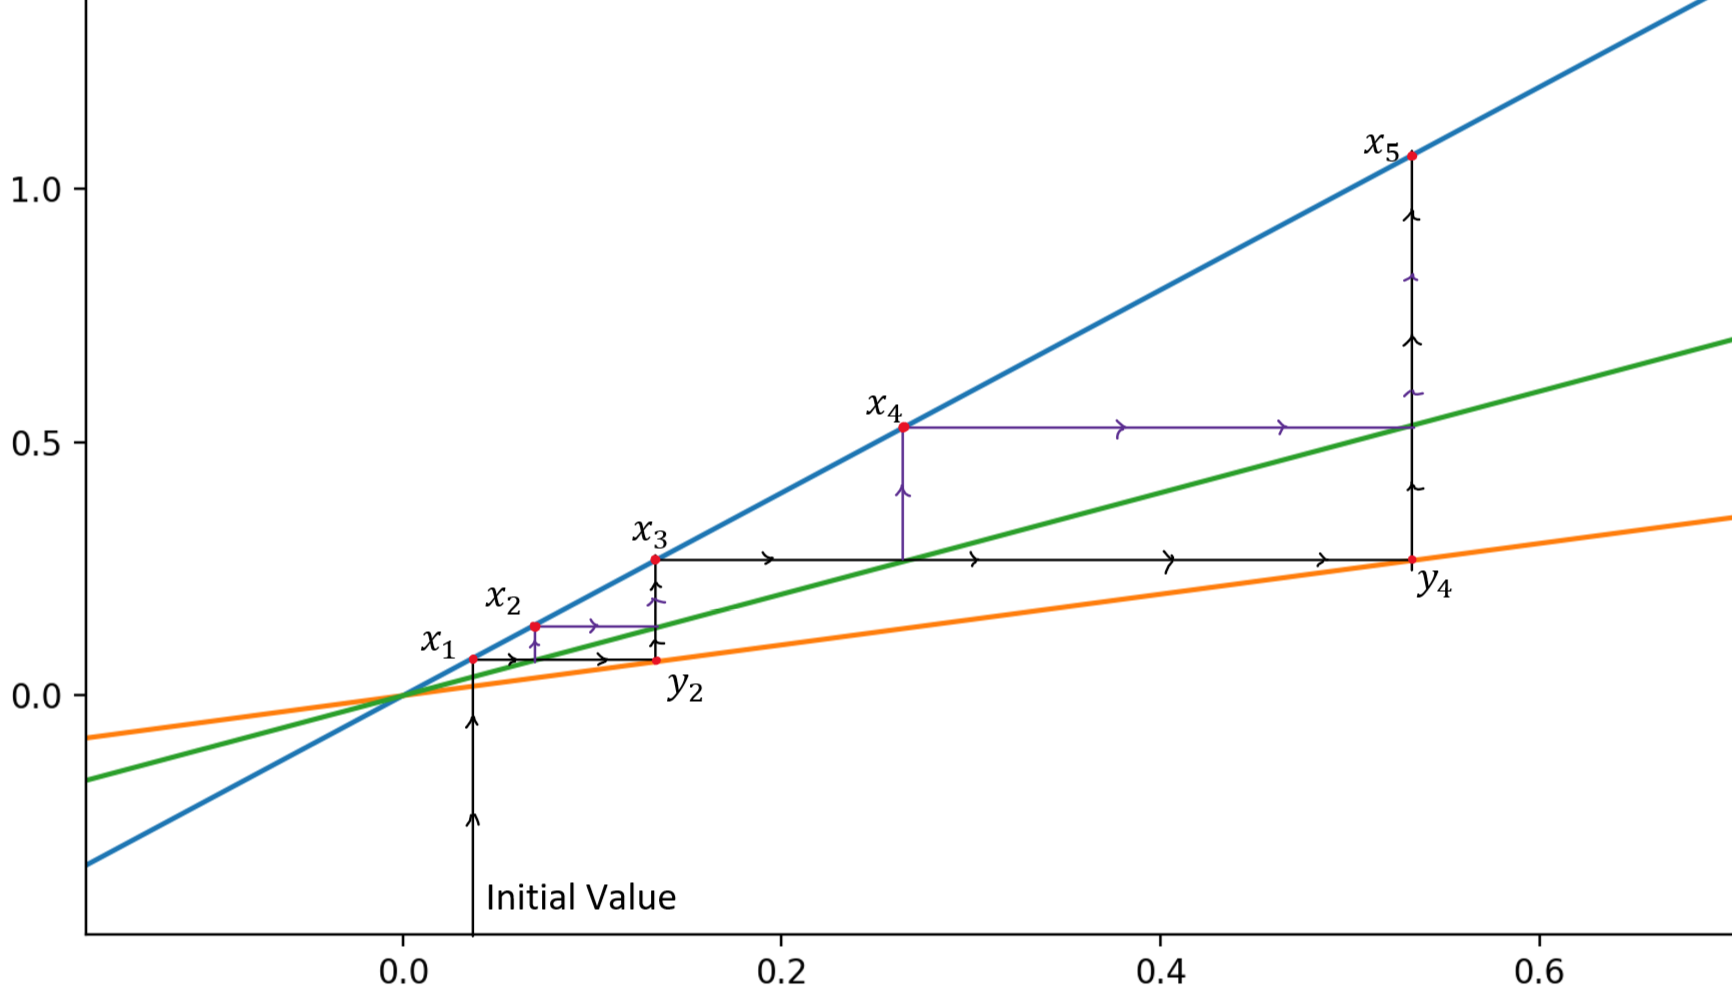
\includegraphics[width=0.6\textwidth]{figure/section1/cobweb-plot.png} \\
\caption{An example of cobweb plot and basic principle}\label{cobweb-plow-1}
\end{center}
\end{figure}

In every iteration, the independent and dependent variable exchanged their location and we can found a group of $\{x_1, y_2, x_3, y_4, \ldots\}$ as orbit of initial value. Or, with the symmetric line $y = x$, it is simple to symmetric all black line to purple line and we can build a cobweb plot with origin image and $y = x$ to find a group of $\{x_1, x_2, \ldots\}$ as orbit from the initial value.

Before we discuss the different of fixed point, it is necessary to review some basic definitions.

\begin{definition}\textbf{$\varepsilon$ Neighbourhood}
\\\noindent In a metric space $X$, an $\varepsilon$ neighbourhood $N_\varepsilon(p)$ of point $p$ is defined 
$$
N_\varepsilon(p) = \{x \in X | d(x, p) < \varepsilon\}
$$
where $d(x, p)$ is the distance bewteen point $p$ and $x$. Also, in a $R^1$ space, the $\varepsilon$ Neighbourhood is give by
$$
N_\varepsilon(p) = \{x \in R | |x-p| < \varepsilon\}
$$
\end{definition}


\newpage

\begin{figure}[H]
\begin{minipage}[c][0.6\width]{
   0.5\textwidth}
   \centering
   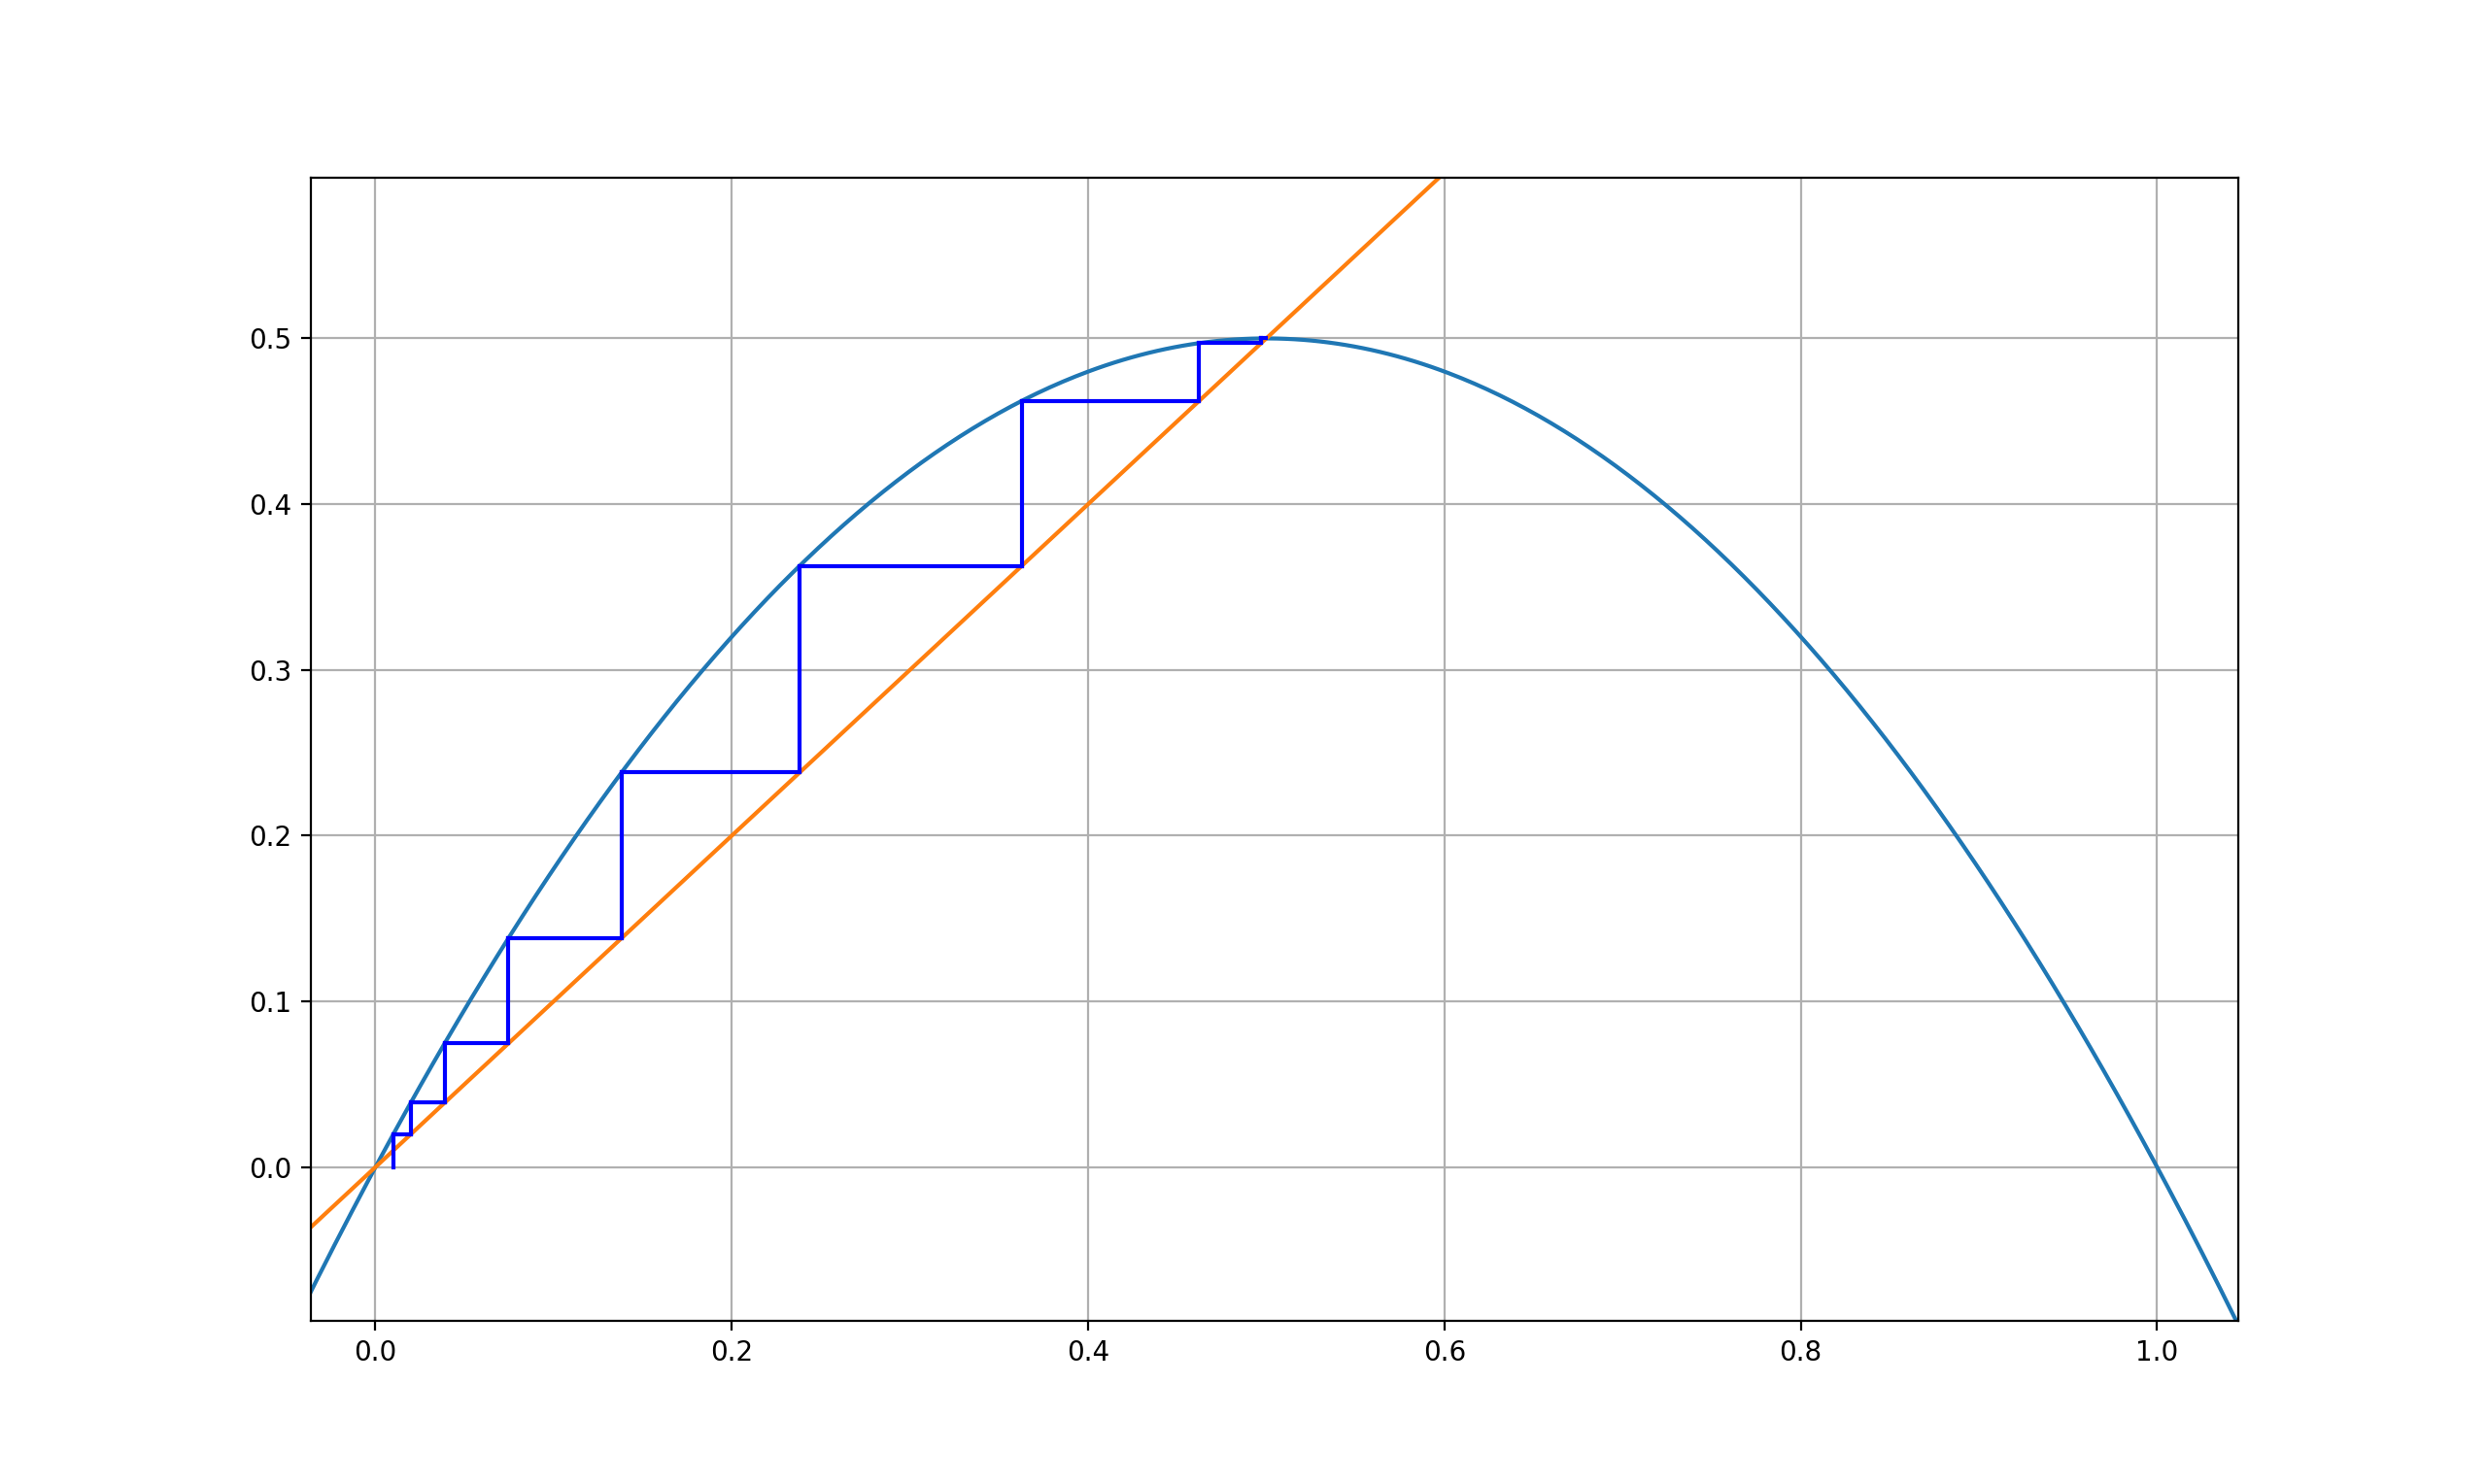
\includegraphics[width=1\textwidth]{figure/section1/cb01.png}
\end{minipage}
\begin{minipage}[c][0.6\width]{
   0.5\textwidth}
   \centering
   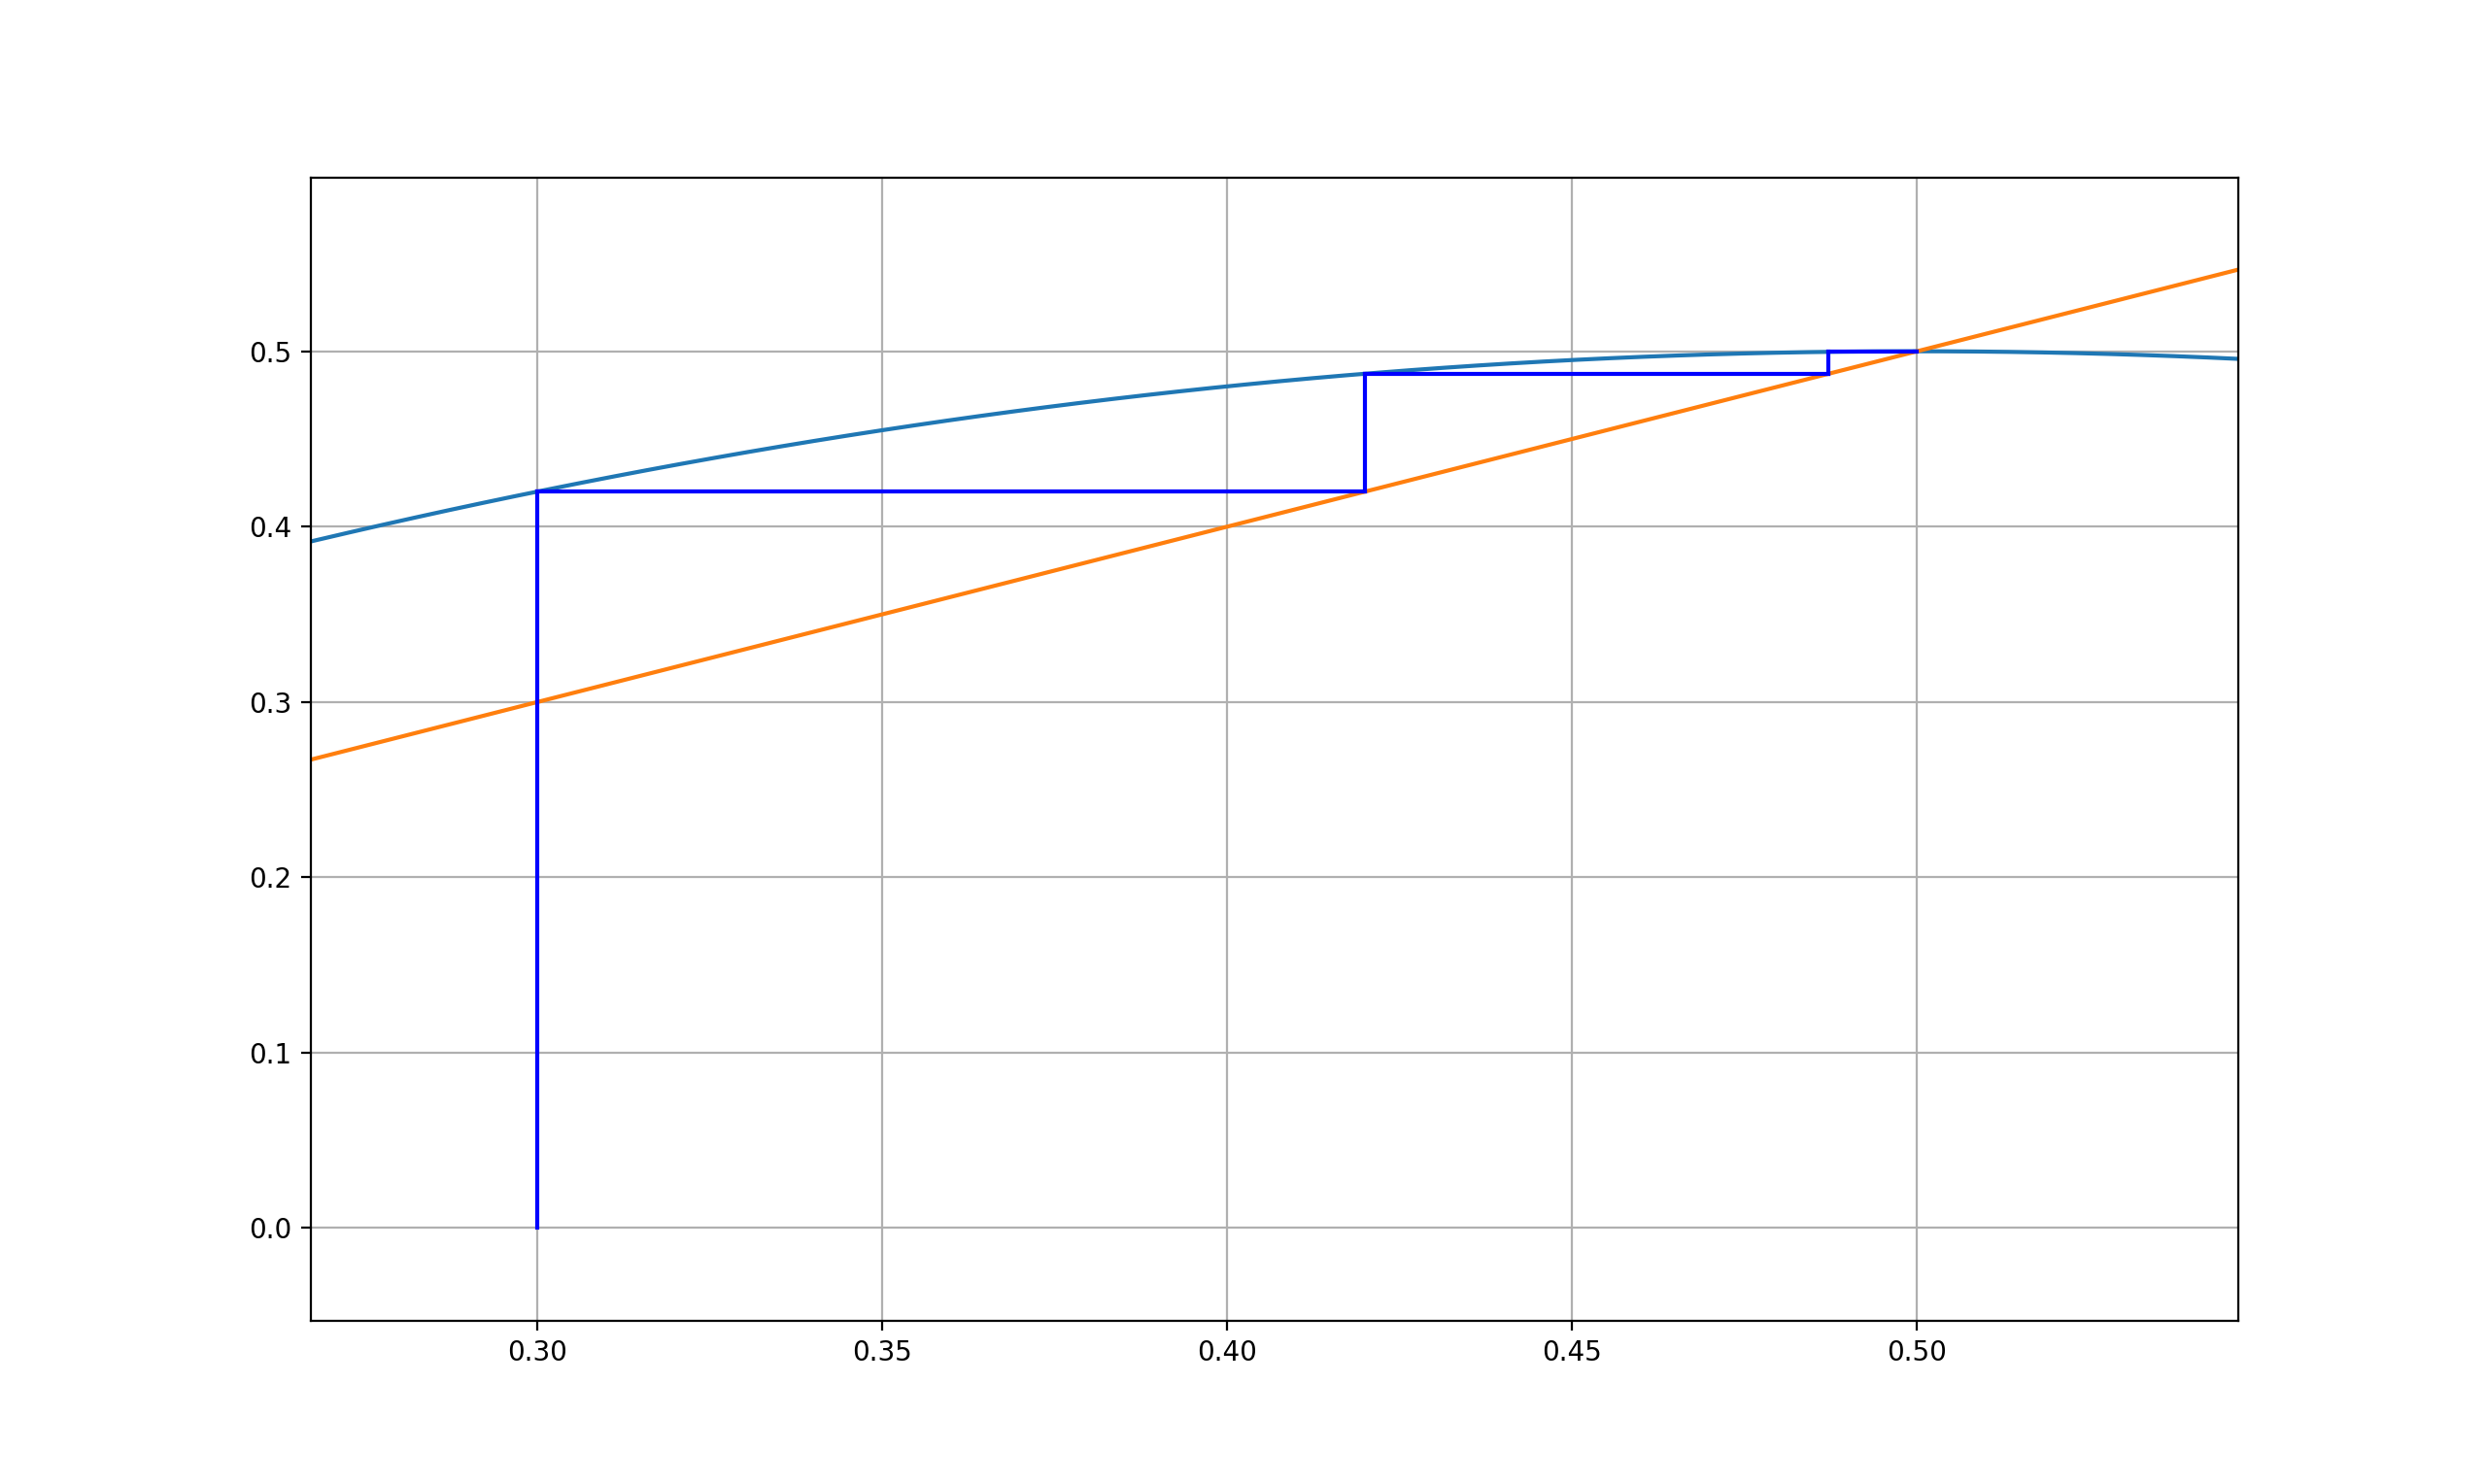
\includegraphics[width=1\textwidth]{figure/section1/cb02.png}
\end{minipage}
\begin{minipage}[c][0.6\width]{
   0.5\textwidth}
   \centering
   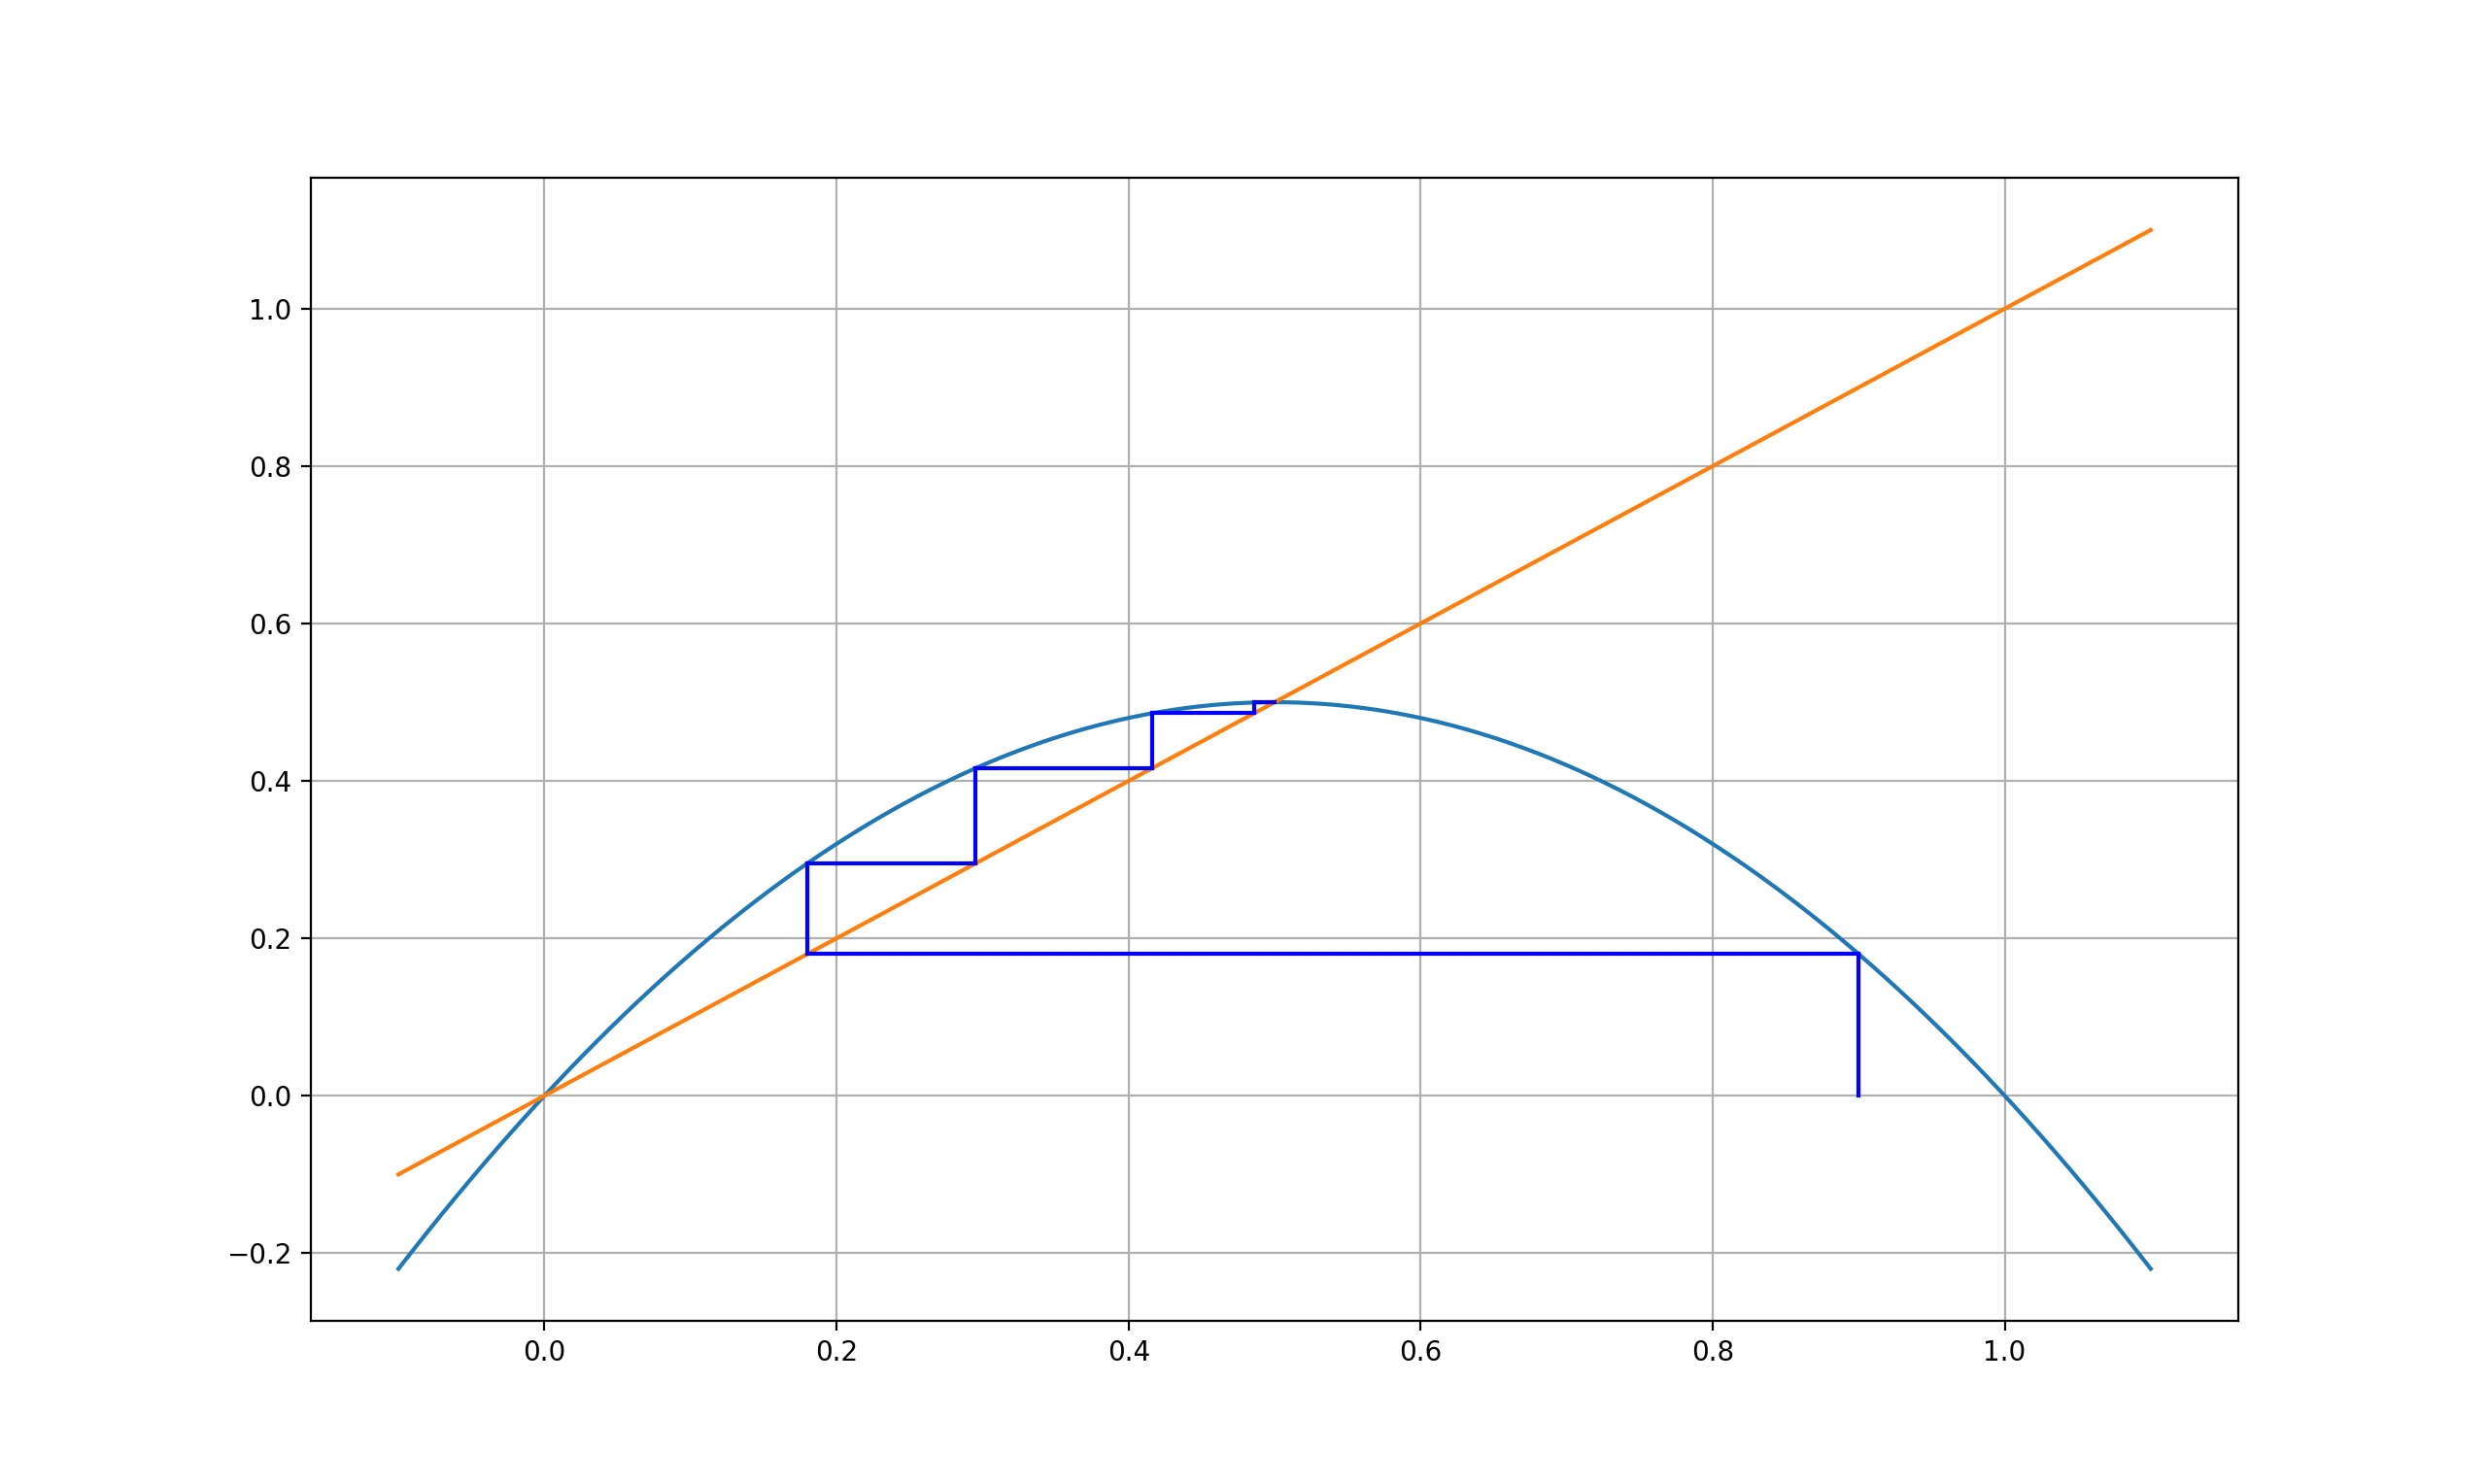
\includegraphics[width=1\textwidth]{figure/section1/cb03.png}
\end{minipage}
\begin{minipage}[c][0.6\width]{
   0.5\textwidth}
   \centering
   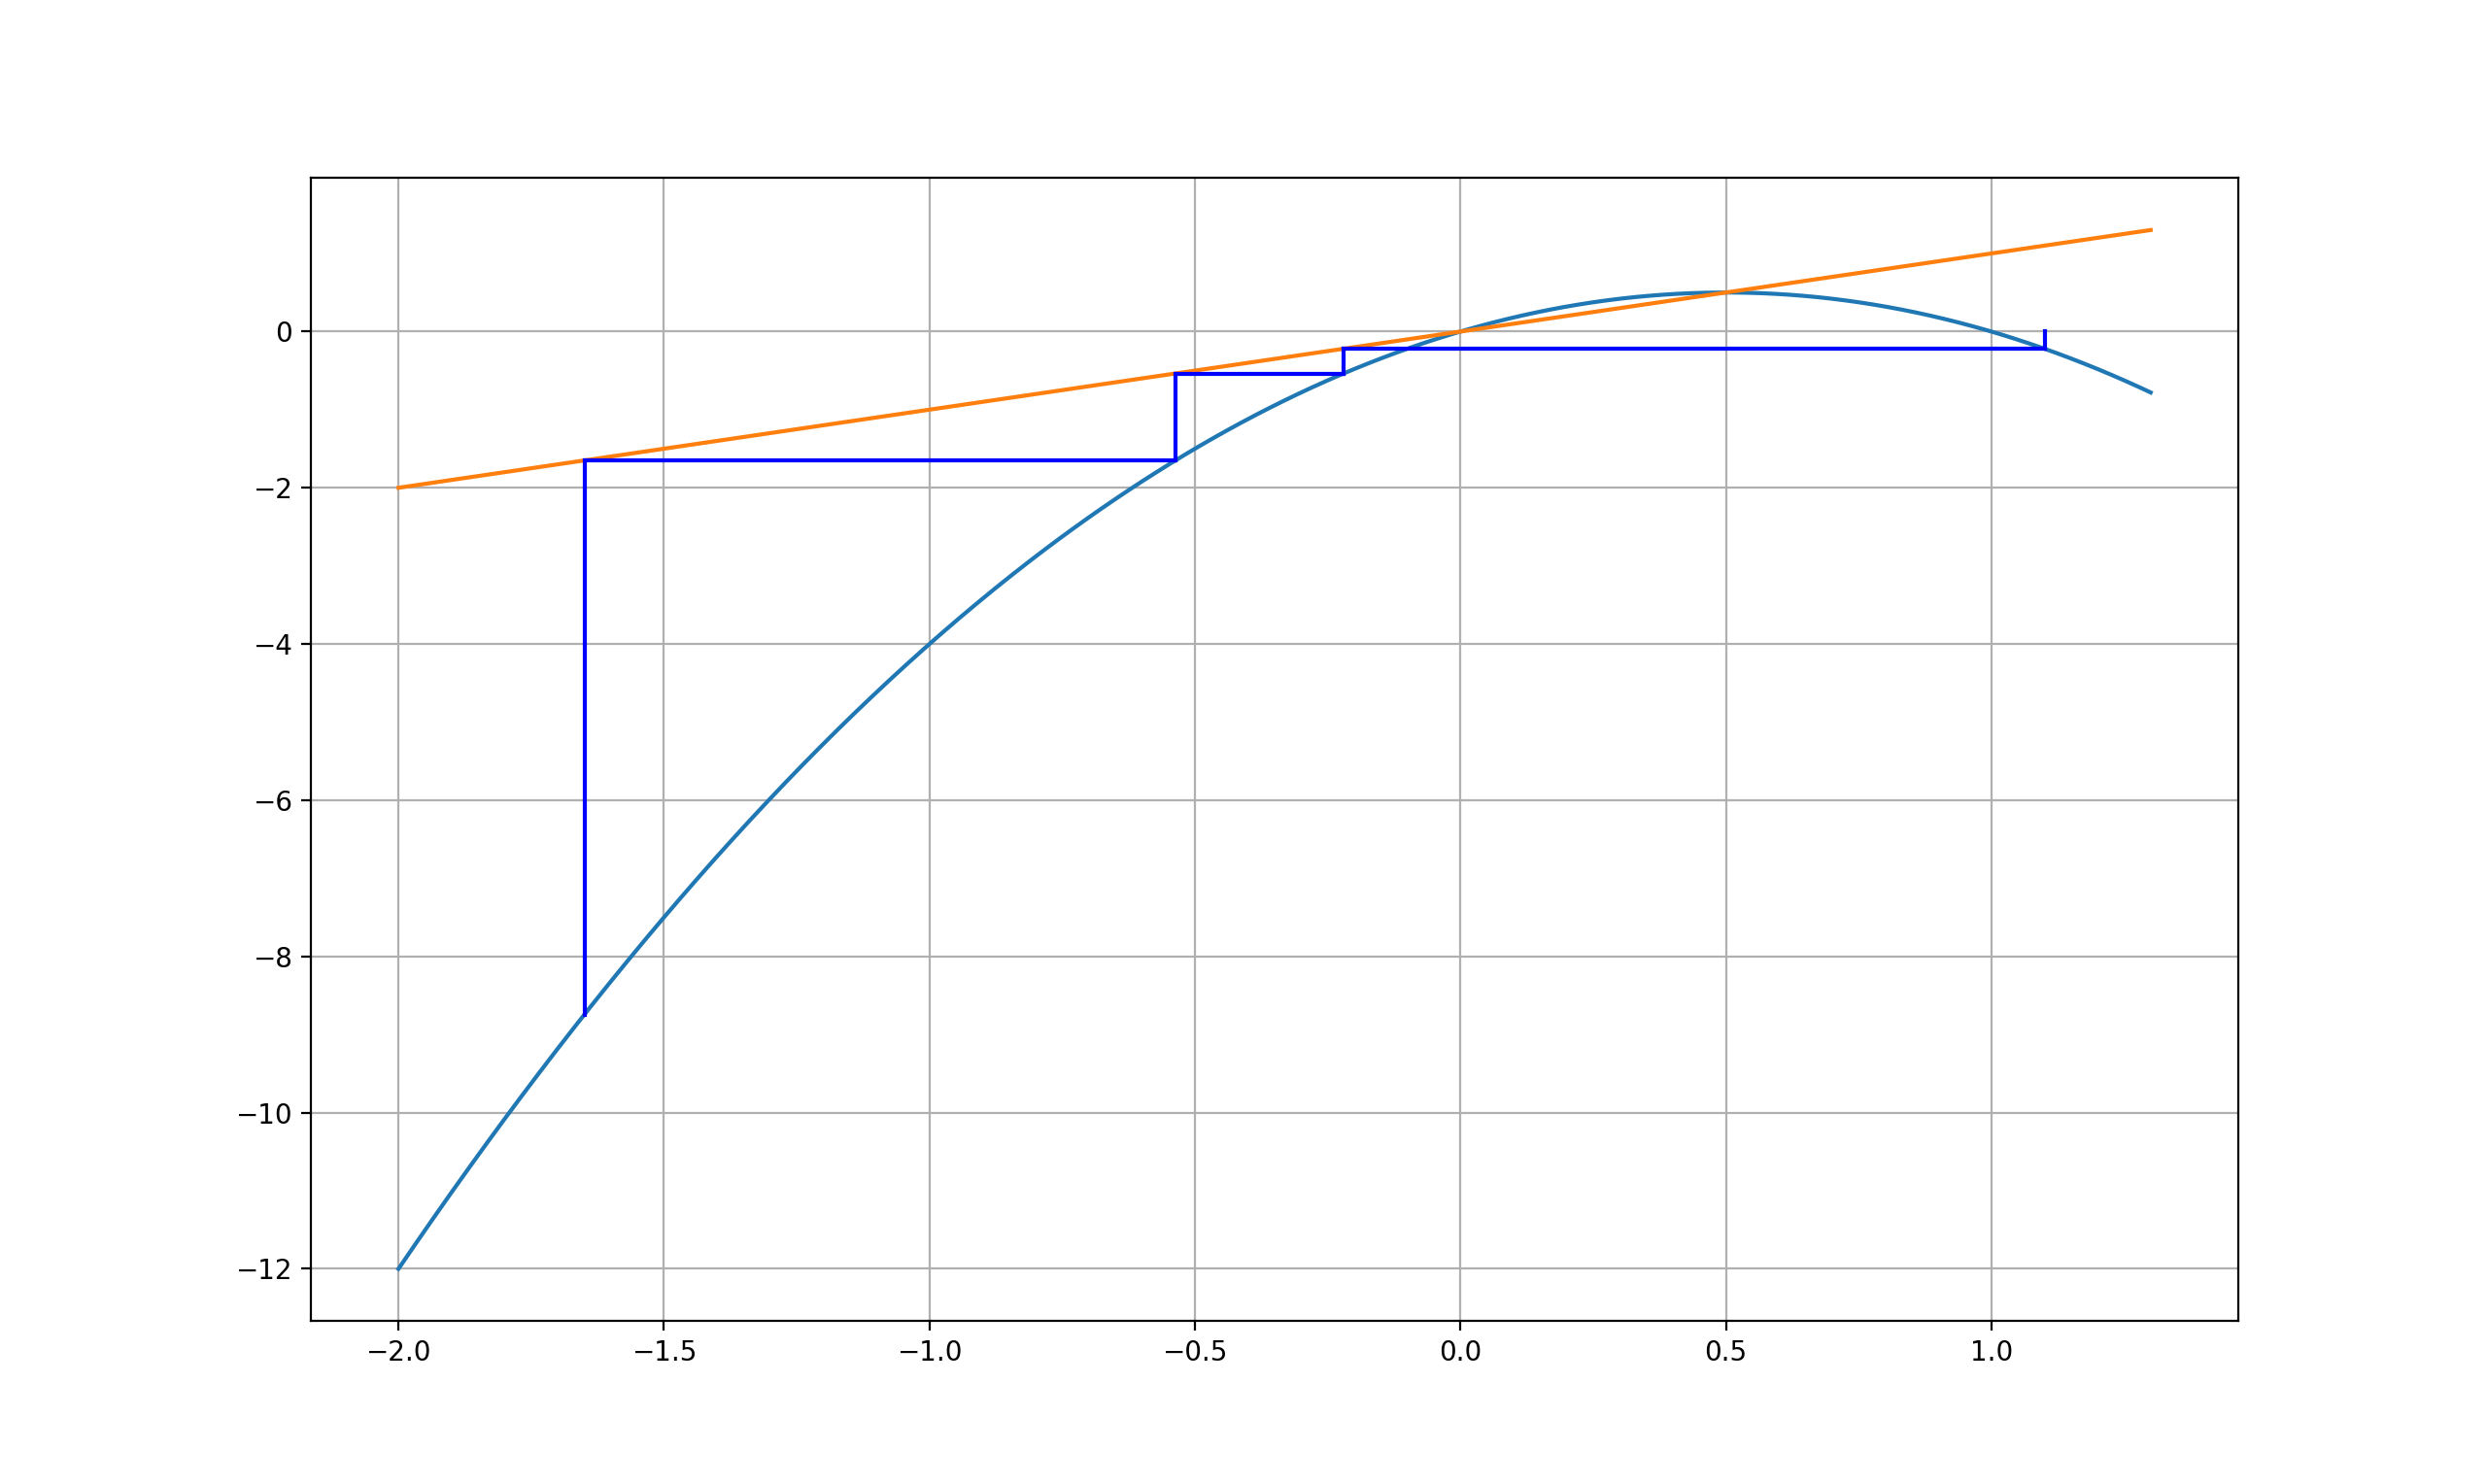
\includegraphics[width=1\textwidth]{figure/section1/cb04.png} \\
\end{minipage}
\caption{Cobweb plot in different initial value}\label{logistic-cobweb-plot}
\end{figure}


It is simple to find that for all initial value $x \in (0, 1)$, with iteration, the output have limitation in 0.5. On the other hand, to solve the equation $x = 2x(1-x)$ we found $x_1 = 0, x_2 = 1, x_3 = 0.5$ as three fixed point. So we have two kinds of fixed point, the one is limitation point and the other is not.


\begin{definition}\textbf{Sink, Source (Attracting and Repelling Fixed Point)}
\\\noindent Consider a map $f: R \rightarrow R$ and point $p$ s.t. $f(p) = p$, then
\\\noindent If for evert points sufficiently to $p$ are attracted to $p$, then called $p$ as \textbf{sink}, or \textbf{attracting fixed point}. Or
$$
\text{For an } \varepsilon > 0, \forall x \in N_\varepsilon(p), \lim_{k \rightarrow \infty}f^k(x) = p \text{ then called } p \text{ as \textbf{sink}}.
$$
If for every points sufficiently to $p$ are repelled to $p$, then called $p$ as \textbf{source}, or \textbf{repelling fixed point}.
$$
\text{For an } \varepsilon > 0, \forall x \in N_\varepsilon(p), x \neq p, \lim_{k \rightarrow \infty}f^k(x) \notin N_\varepsilon(x) \text{ then called } p \text{ as \textbf{source}}.
$$
\end{definition}



\newpage

\begin{theorem} \label{sink-source-point}Let $f$ is a map on $R$, assume $p$ is a fixed point of $f$, then
\\\noindent [i] If $|f'(p)| < 1$, then $p$ is a sink;
\\\noindent [ii] If $|f'(p)| > 1$, then $p$ is a source.
\end{theorem}


{\color{blue}
\begin{proof} \textbf{[i]} Based on definition of derivative, we have
$$
\lim_{x \rightarrow p} {|f(x) - f(p)| \over |x - p|} = |f'(p)|
$$
Now. let $a \in (\min(|f'(p)|, 1), \max(|f'(p)|, 1))$ (e.g. $a = {1\over 2}(1+ |f'(p)|)$), then
$$
\forall a \in (\min(|f'(p)|, 1), \max(|f'(p)|, 1)), \exists \varepsilon_0 > 0 \text{ s.t. } \forall \varepsilon \in (0, \varepsilon_0], \forall x \in N_\varepsilon(p), {|f(x) - f(p)| \over |x - p|} < a
$$
            \textit{That means, $f(x)$ is closer to $p$ than $x$ (or distant bewteen curve $y = f(x)$ and $y = x$), but at least a factor of $a$ and we have the conclusion
$$
\forall x \in N_\varepsilon(p), f(x) \in N_\varepsilon(p)
$$
            During the iteration processing it is simple to find that all orbit $\{f(x), f^2(x), \ldots f^n(x), \ldots\} \subset N_\varepsilon(p)$, so now we can consider another conclusion in follow.}
\\[2ex]\noindent \textbf{[ii]} We try to prove the inequality $\forall x \in N_\varepsilon(p), |f^k(x) - p|$
\\\noindent \textbf{[ii-1]} Obvious, if $k = 1$, then $|f(x) - p| = |f(x) - f(p)| < a |x-p|$ ($p$ is fixed point so $f(p) = p$)
\\\noindent \textbf{[ii-2]} If $k = 2$, Based on the conclusion in \textbf{[i]}, $x_1 = f(x) \in N_\varepsilon(p)$ and $|f(x_1) - p| < a |x_1 - p| < a^2 |x - p|$
\\\noindent $\ldots$
\\\noindent \textbf{[ii-k+1]} (Assume the inequality is established in $k$), then
$$
|f^{k+1}(x) - p| < a|f^k(x) - p| < a \cdot a^k |x - p| = a^{k+1}|x - p|
$$
            In summary, for all $k \in N$, the inequality is established.
\\[2ex]\noindent \textbf{[iii-1]} Now we consider the equality condition, if $|f'(p)| < 1$ then $a < 1$ and  
$$
\lim_{k \rightarrow \infty}|f^{k}(x) - p| < |x-p|\lim_{k \rightarrow \infty} a^k = 0 \text{ (Because }a \in (0, 1)\text{)} 
$$
            So we have the conclusion, 
$$
\forall x \in N_\varepsilon(p), \lim_{k \rightarrow \infty}f^k(x) = p
$$
            \textbf{[iii-2]} Also, if $|f'(p)| > 1$ then $a^k \rightarrow \infty$, that means, with the iteration, the maps will eventually outside the condition, or the domain interval. $\blacksquare$
\end{proof}
}

* We will discuss what happened while $f'(p) = 1$ laterly.

** Obviously, this theorem expressed a kind of convergence, as the speed of the convergence is based on the $a$ in exponent function, we called this convergence as \textbf{Exponential Convergence}.

Now we consider another map as example.


\newpage
\begin{example} Solved the fixed point of $\varphi(x) = (3x -x^2)/2$, find every sink and source point with Theo. \ref{sink-source-point}
\end{example}


\begin{figure}[H]
\begin{center}
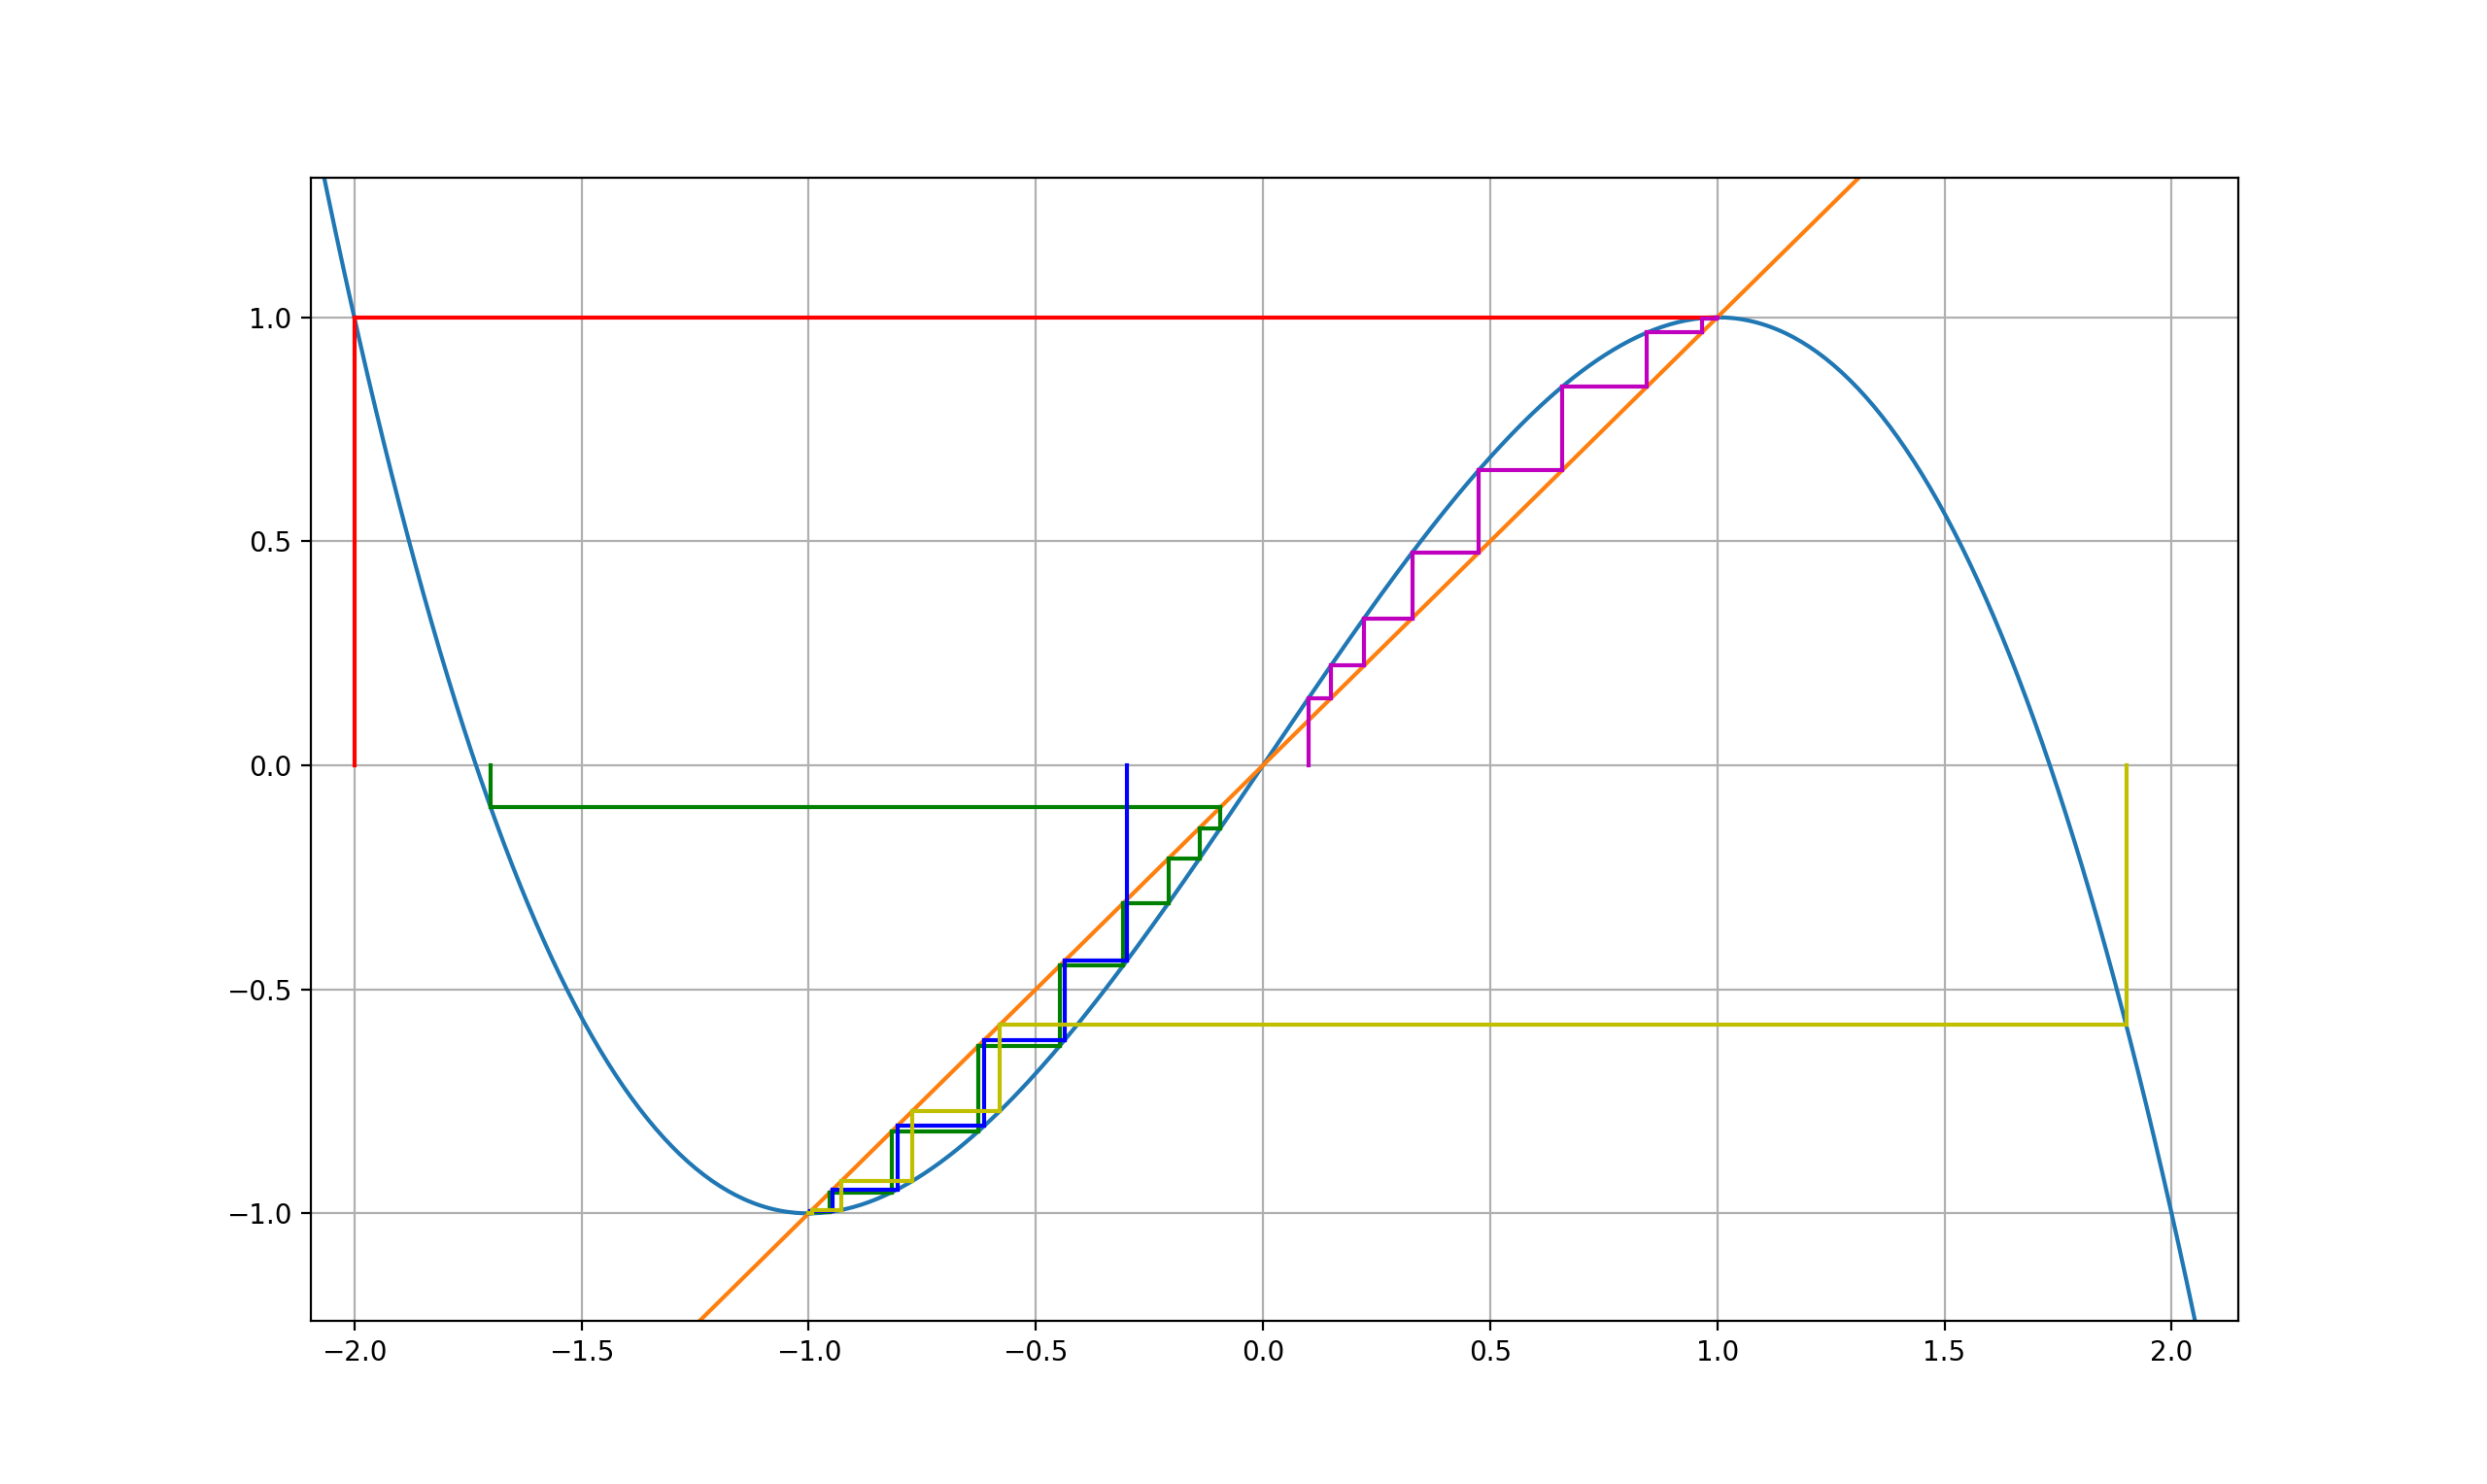
\includegraphics[width=0.5\textwidth]{figure/section1/cobweb-plot-2.png} \\
%\caption{}\label{cobweb-plow-2}
\end{center}
\end{figure}

{\color{blue}
\begin{solution}
It is simple to find the fixed point with $x = (3x - x^3) / 2$ and $x_1 = 1, x_2 = 0, x_3 = -1$. Based on the image, we can found that $1$ and $-1$ are sink and $0$ is source. On the other hand
$$
\varphi'(x) = {3\over 2} (1 - x^2), \varphi'(-1) = 0 < 1, \varphi'(0) = {3 \over 2} > 1, \varphi'(1) = 0 < 1
$$ 
and we proved the conclusion we found on figure before. $\blacksquare$
\end{solution}
}

Another way to confirm a point is sink or source is based on the formula identity and algebra. For instance, we consider the distance bewteen $g(x) = 2x(1-x)$ and fixed point $1/2$, then 
$$
|g(x) - 1/2| = |2x(1-x) - 1/2| = 2|x - 1/2||x - 1/2|
$$

and $\forall x \in (0, 1), |x - 1/2| < 1 \Rightarrow |g(x) - 1/2| < 1$, that means the distance bewteen $g(x)$ and $p$ is decreasing during time iteration and we can confirm that $1/2$ is a sink point rather than source point.

Next, we will focus on a logistic model with different parameter.








\subsection{Periodic points, family of logistic maps}
\begin{example} Find the fixed point of $g(x) = 3.3x(1-x), x \in [0, 1]$.
\end{example}

{\color{blue}
\begin{solution}
It is simple to find the fixed point with $x = 3.3x(1-x)$ and $x_1 = 0, x_2 = 23/33, x_3 = 1$. Obviously, both 0 and 1 are source. And
$$
g'(x) = 3.3 - 6.6x, |g'(23/33)| = 1.3 > 1
$$ 
So all these three fixed point are source, and it is simple to find the conclusion with cobweb plot. $\blacksquare$
\end{solution}
}

\newpage
\begin{figure}[H]
\begin{center}
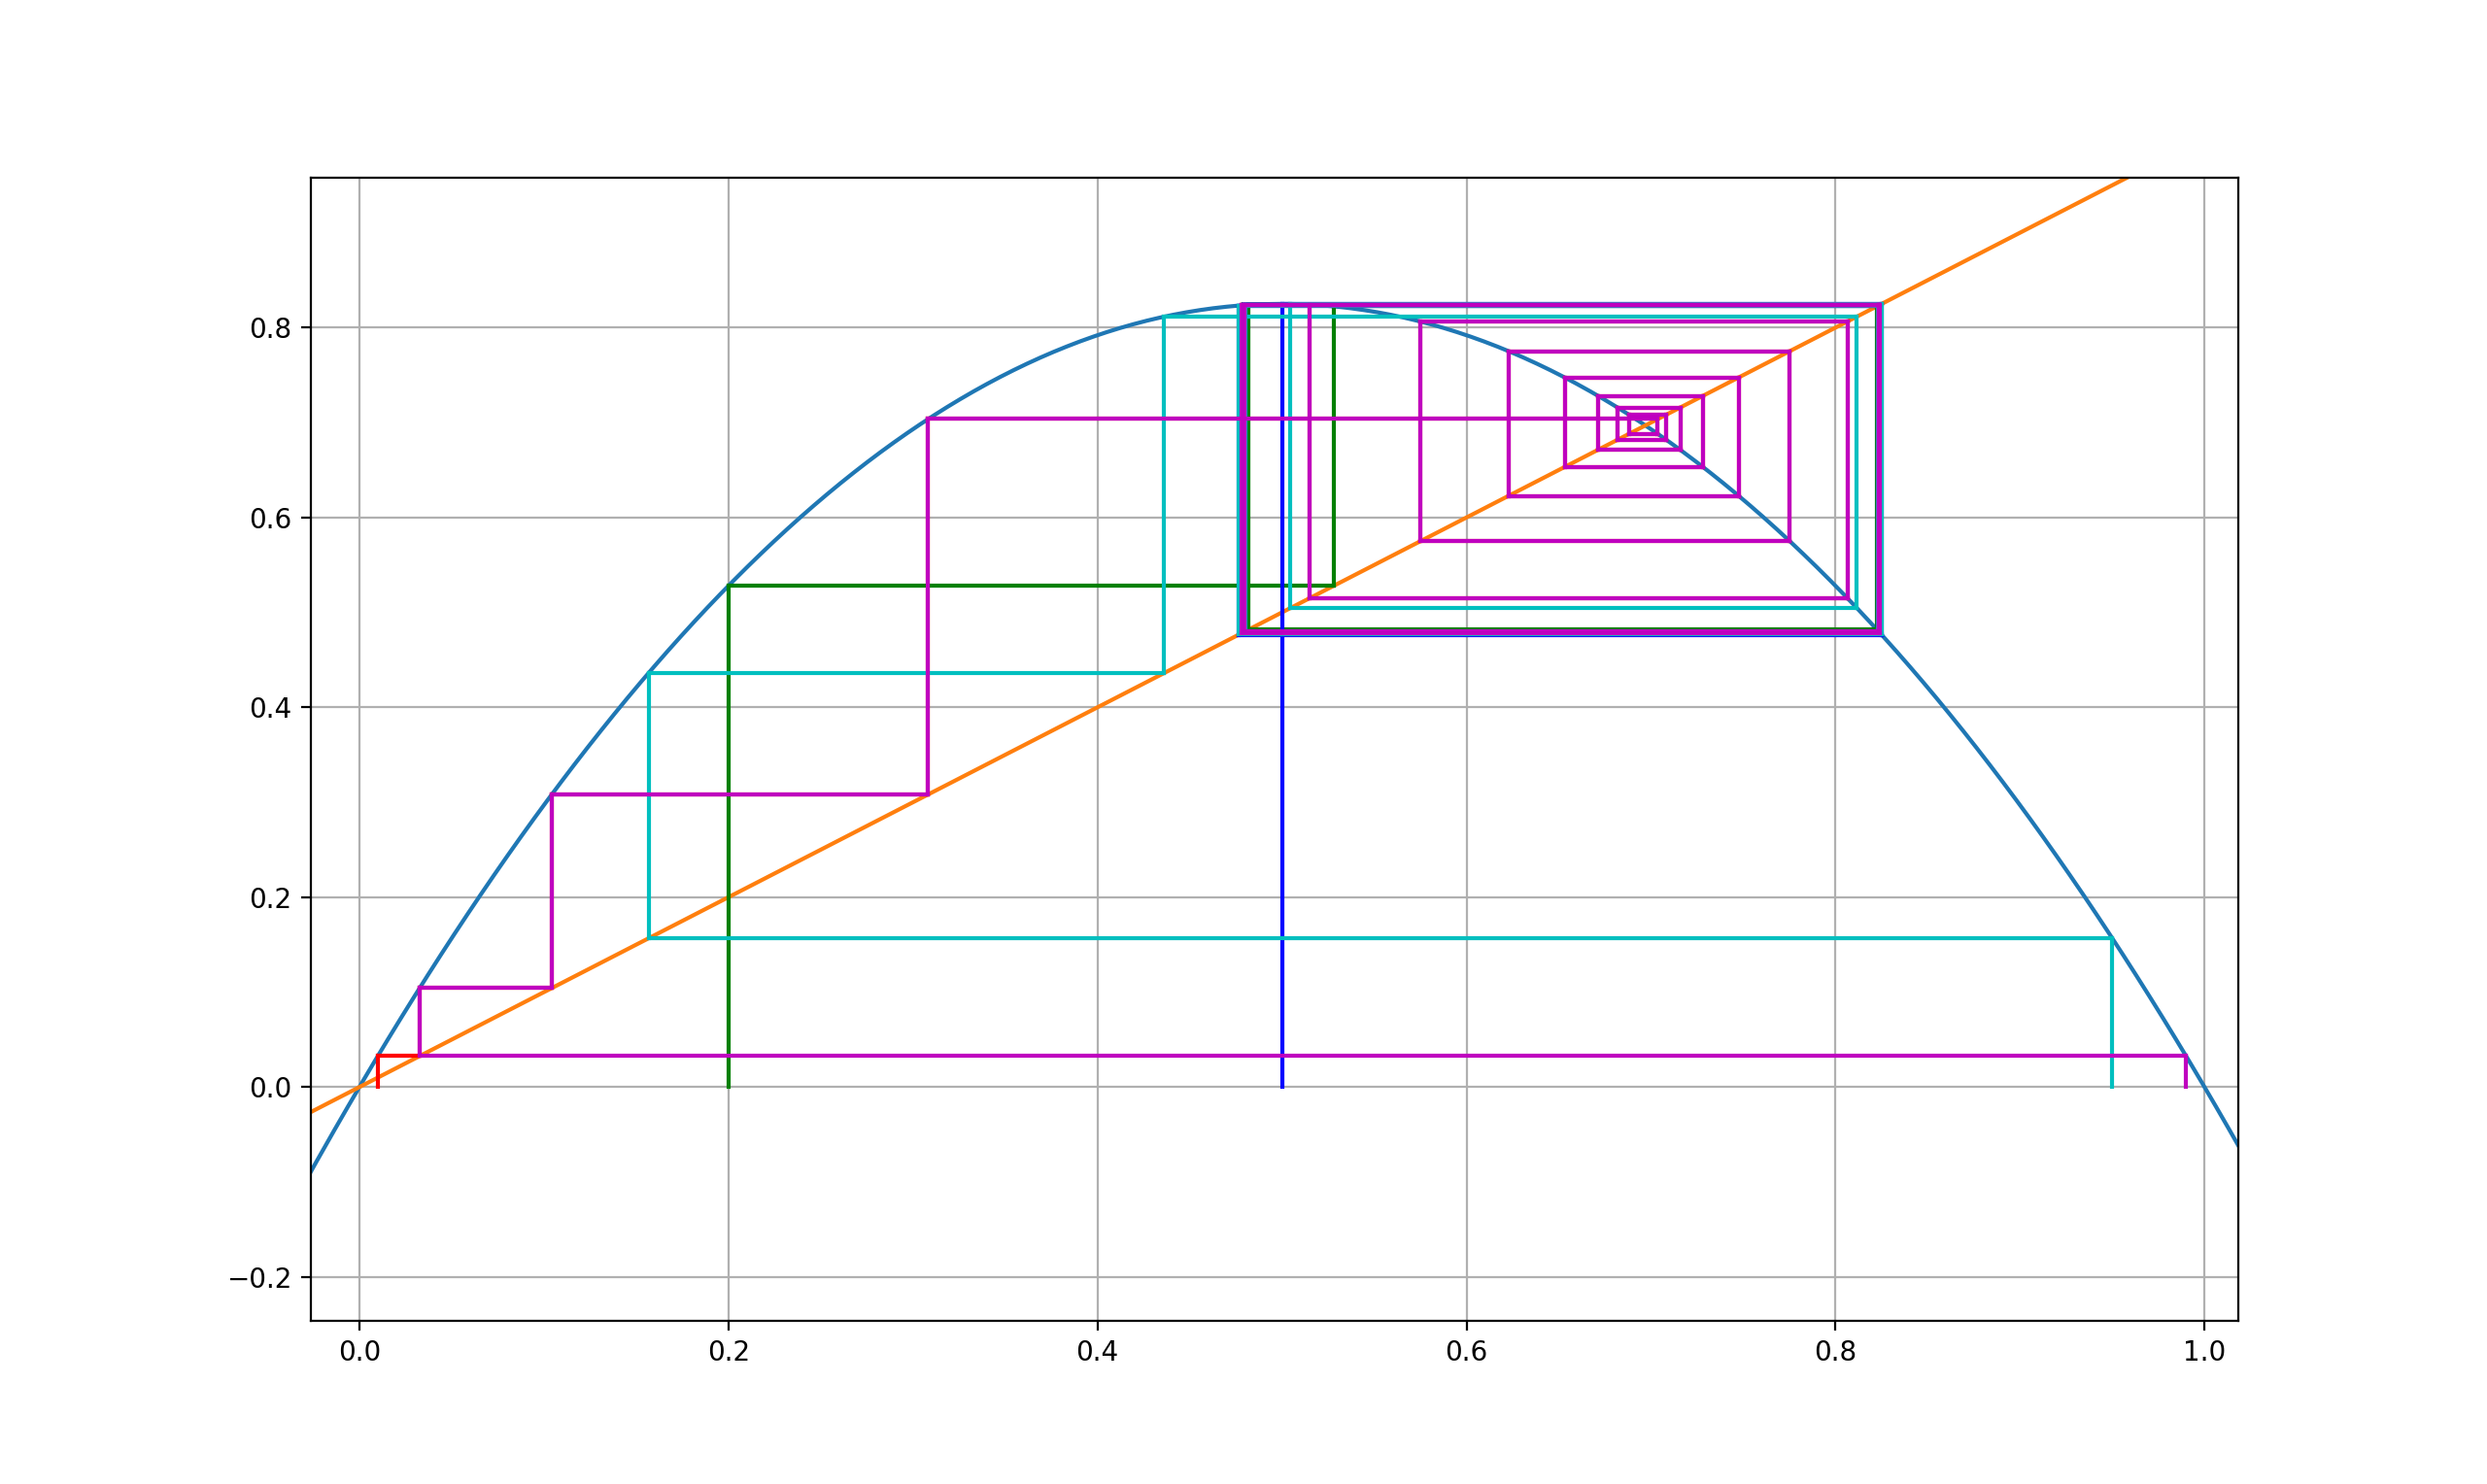
\includegraphics[width=0.6\textwidth]{figure/section1/periodic-point.png} \\
\caption{An example of periodic point}\label{periodic-point}
\end{center}
\end{figure}


Hold on a second, something strange! Even we cannot find a sink fixed point, all of initial value are sank into a group of points!

\begin{definition}\textbf{Period-k point, Period-k orbit}
\\\noindent Let $f$ be a map on $R$, and $p$ is a point in domain, if $f^k(p) = p$, and $k$ is the smallest such positive integer, then called $p$ as \textbf{periodic point of period $k$}, or \textbf{period-k point};
\\\noindent Called orbit with initial point $p$ as \textbf{periodic orbit of period k}, or \textbf{period-k orbit};
\end{definition}

\begin{definition}\textbf{Sink and Source in Period point}
\\\noindent Let $f$ be a map and $p$ is a period-k point
\\\noindent If $p$ is a sink, then called this period-k orbit as periodic sink;
\\\noindent If $p$ is a source, then called this period-k orbit as periodic source.
\end{definition}

Obviously, based on the chain rule, we have $(fg)'(x) = f'(g(x))g'(x)$, let $f = g, x = p_1$, then 
$$
g^2(p_1) = g'(g(p_1))g'(p_1) = g'(p_2)g'(p_1)
$$
Summary this formula, we have 
\begin{theorem} \label{chain-rule-period-orbit}For every map $f$ and period-k orbit $\{p_1, p_2, \ldots p_k\}$, 
$$
(f^k)'(p_1) = (f^k)'(p_2) = \ldots = (f^k)'(p_k) = \prod_{i = 1}^{k}f'(p_i)
$$
\end{theorem}

{\color{blue}
\begin{proof} \textbf{Theo. \ref{chain-rule-period-orbit}} 
$$
(f^k)(p_1) = (f(f^{k-1}))'(p_1) = f'(f^{k-1}(p_1))(f^{k-1})'(p_1) = \ldots = \prod_{i = 1}^{k}f'(p_i) = (f^k)(p_i) (\forall i = 1, 2, \ldots, k)\blacksquare
$$
\end{proof}
}

\newpage
Same as Theo. \ref{sink-source-point}, we have stability test for periodic orbits.
\begin{theorem}\label{stability-test-for-periodic-orbits}\textbf{Stability test for periodic orbits}
\\\noindent Let $f$ is a map and period-k orbit $\{p_1, p_2, \ldots p_k\}$, 
\\\noindent If $|\prod_{i = 1}^{k}f'(p_i)| < 1$ then called this periodic orbit is a sink;
\\\noindent If $|\prod_{i = 1}^{k}f'(p_i)| > 1$ then called this periodic orbit is a source;
\end{theorem}


{\color{blue}
\begin{proof} \textbf{Theo. \ref{sink-source-point}} 
\\\noindent Consider a new map $g(x) = f^k(x)$, where $f$ be a map and $p$ is a period-k point, then $p$ is a fixed point of $g$. Based on Theo. \ref{sink-source-point}, $|g(p)| < 1$ if $p$ is sink and $|g(p)| > 1$ if $p$ is a source. On the other hand, $g(p) = f^k(p) = \prod_{i = 1}^{k}f'(p_i) \blacksquare$   
\end{proof}
}

Now we consider another problem.

\begin{example} Find the fixed point or periodic orbit of $g_{3.5}(x) = 3.5x(1-x), g_{3.86}(x) = 3.86x(1-x), x \in [0, 1]$.
\end{example}


\begin{figure}[H]
\begin{minipage}[c][0.5\width]{
   0.5\textwidth}
   \centering
   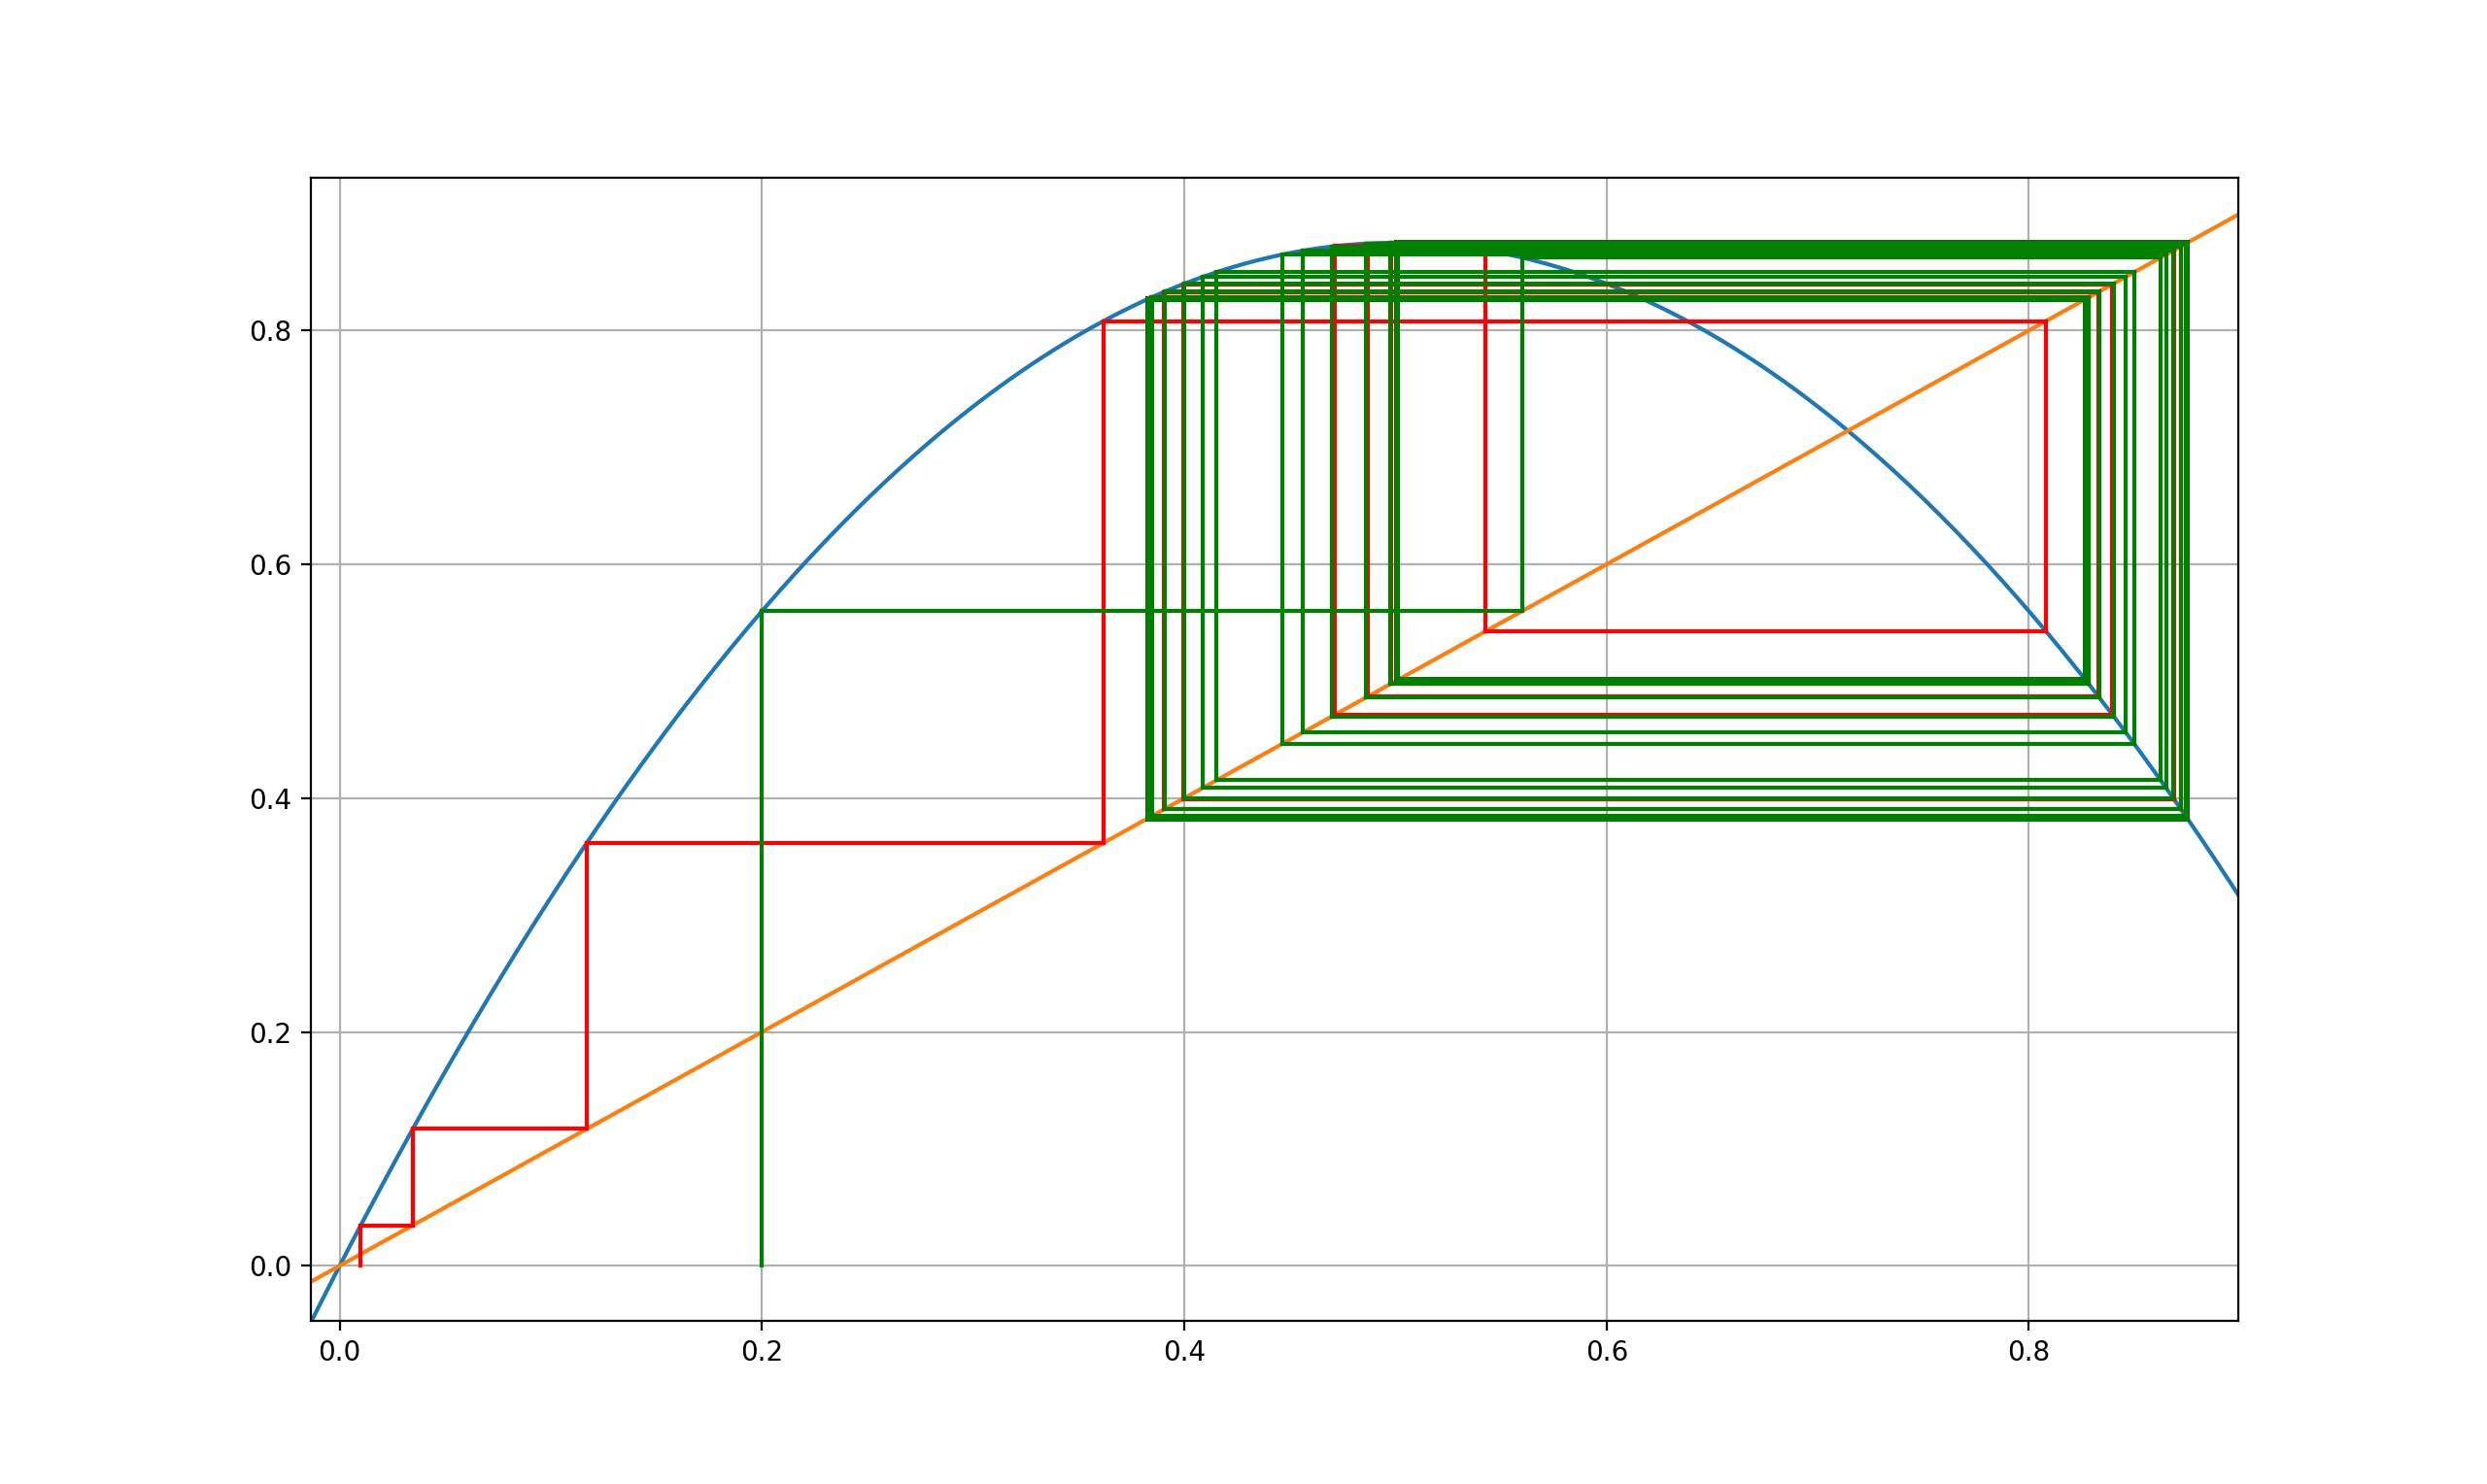
\includegraphics[width=0.9\textwidth]{figure/section1/logistic35.png}
\end{minipage}
\begin{minipage}[c][0.5\width]{
   0.5\textwidth}
   \centering
   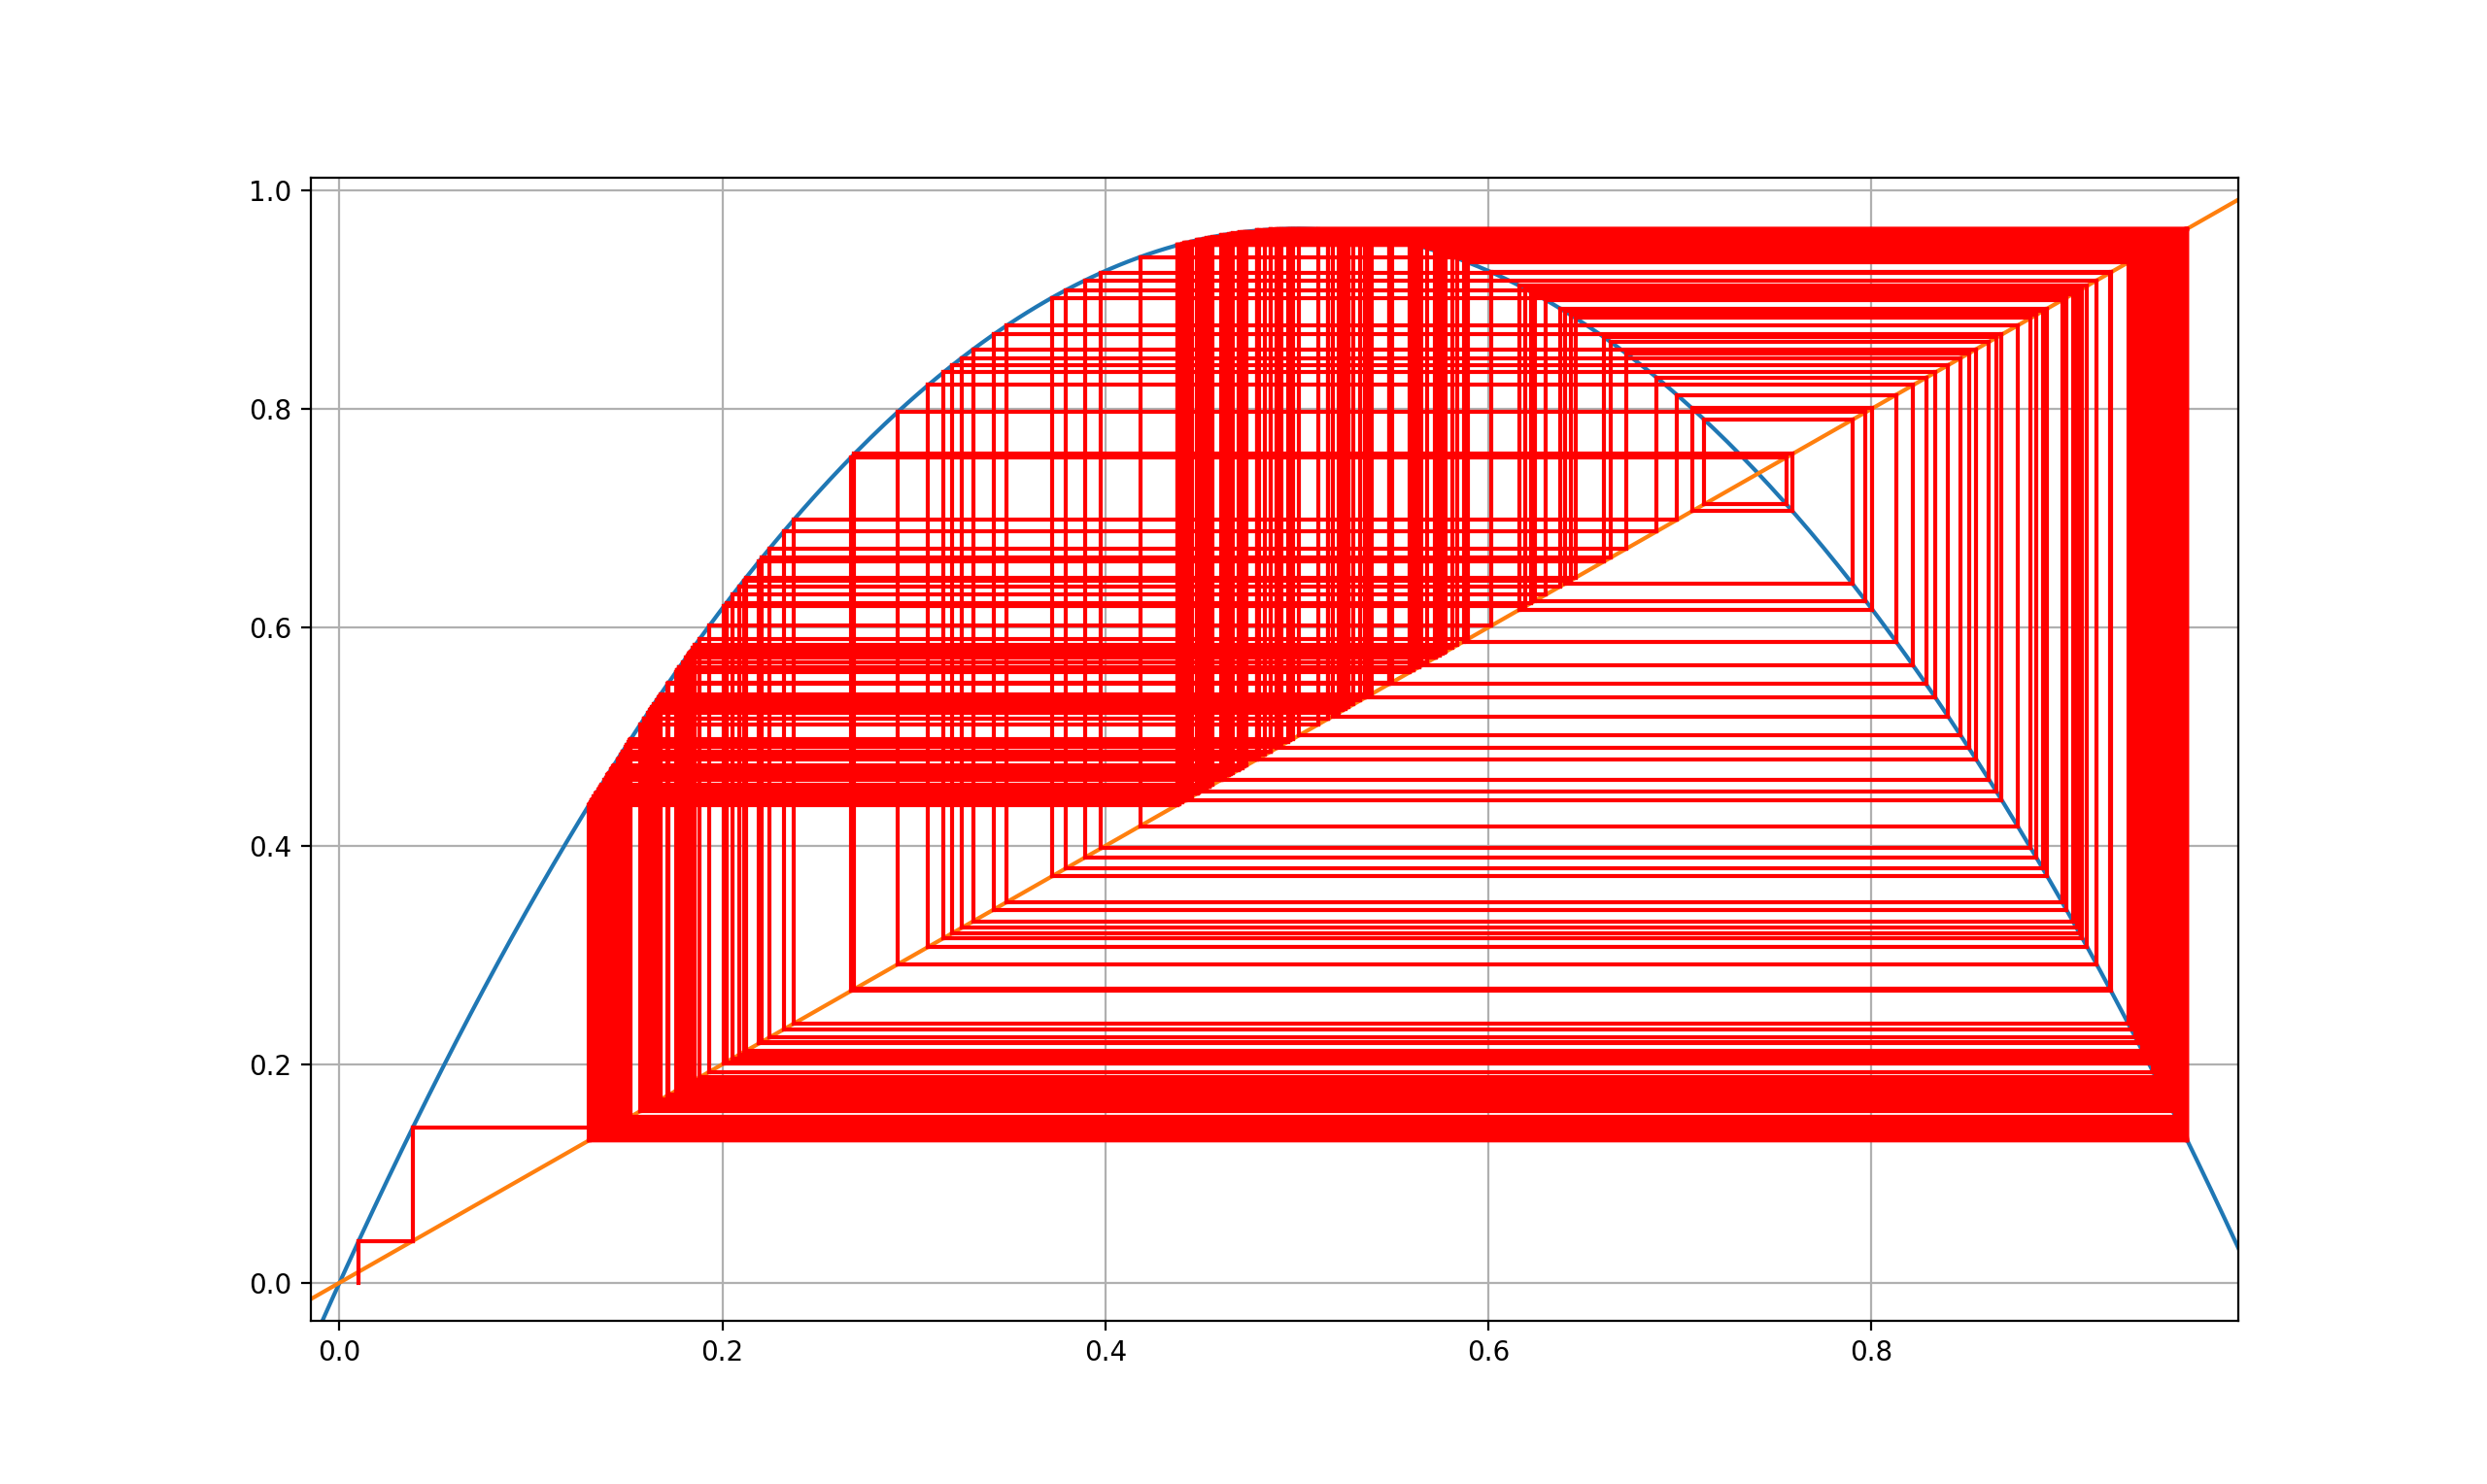
\includegraphics[width=0.9\textwidth]{figure/section1/logistic386.png} \\
\end{minipage}
\caption{Logistic maps in $a = 3.5$ and $a = 3.86$}\label{logistic-no-periodic}
\end{figure}

We found in $a = 3.5$, even the periodic orbit is difficult to find, the iteration still have a boundary. If we consider every $a \in [1, 4]$, we can plot a figure between parameter $a$ and orbits $x$, and this \textbf{bifurcation diagram} was made by following repearting:
\\\noindent \textbf{[i]} Choose a value $a$, starting with $a = 1$.
\\\noindent \textbf{[ii]} Choose a value $x \in [0, 1]$ randomly.
\\\noindent \textbf{[iii]} Calculate the orbit of x under $g_a(x)$ in a certain iteration times $t_max$.
\\\noindent \textbf{[iv]} Ignore the first $t_0$ iterates and plot the orbit.


\begin{figure}[H]
\begin{center}
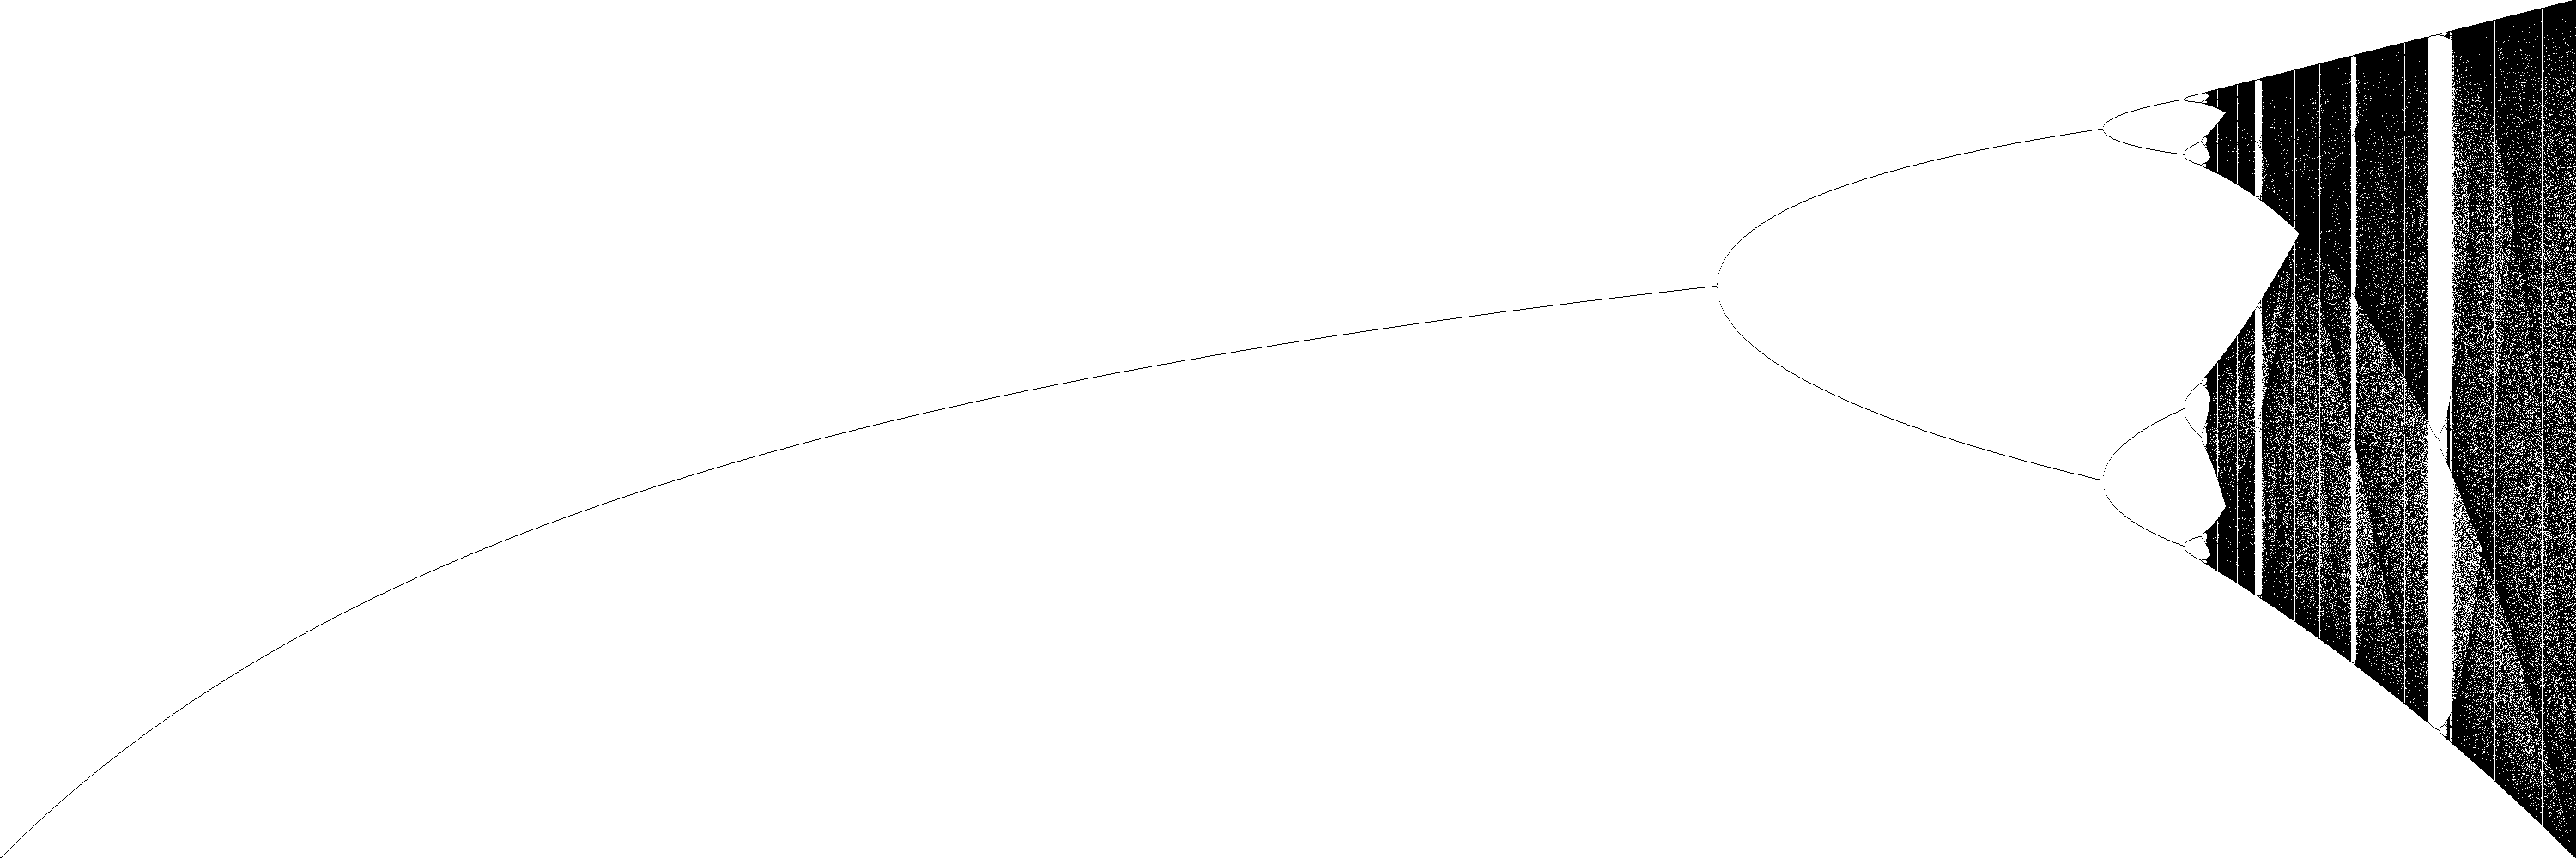
\includegraphics[width=0.4\textheight]{figure/section1/logistic-stability.png} \\
\caption{Logistic model stability interval ($a \in [1, 4]$)}\label{Logistic-stability}
\end{center}
\end{figure}




\newpage
\begin{discussion} Now we will discuss the family of logistic maps with Fig. \ref{Logisstic-stability}
\\\noindent \textbf{[i] Periodic-3 window}
\\\noindent We found periodic-1 orbits (or point) and periodic-2 orbits, based on the image above, it seem we also have periodic-3 orbits. And now we focus on the interval of parameter $a$ rather than domain of function, we found there is a interval of $a$ inside the $[3.83, 3.86]$ and we called these kind of interval as ``periodic window''. For instance, next figure showed the periodic-3 window of $a$.

\begin{figure}[H]
\begin{minipage}[c][0.5\width]{
   0.5\textwidth}
   \centering
   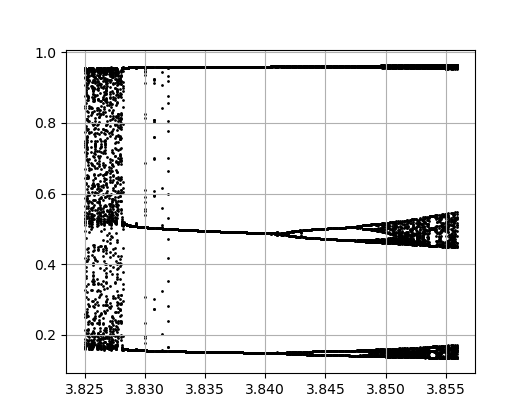
\includegraphics[width=0.70\textwidth]{figure/section1/periodic-3-window.png}
\end{minipage}
\begin{minipage}[c][0.5\width]{
   0.5\textwidth}
   \centering
   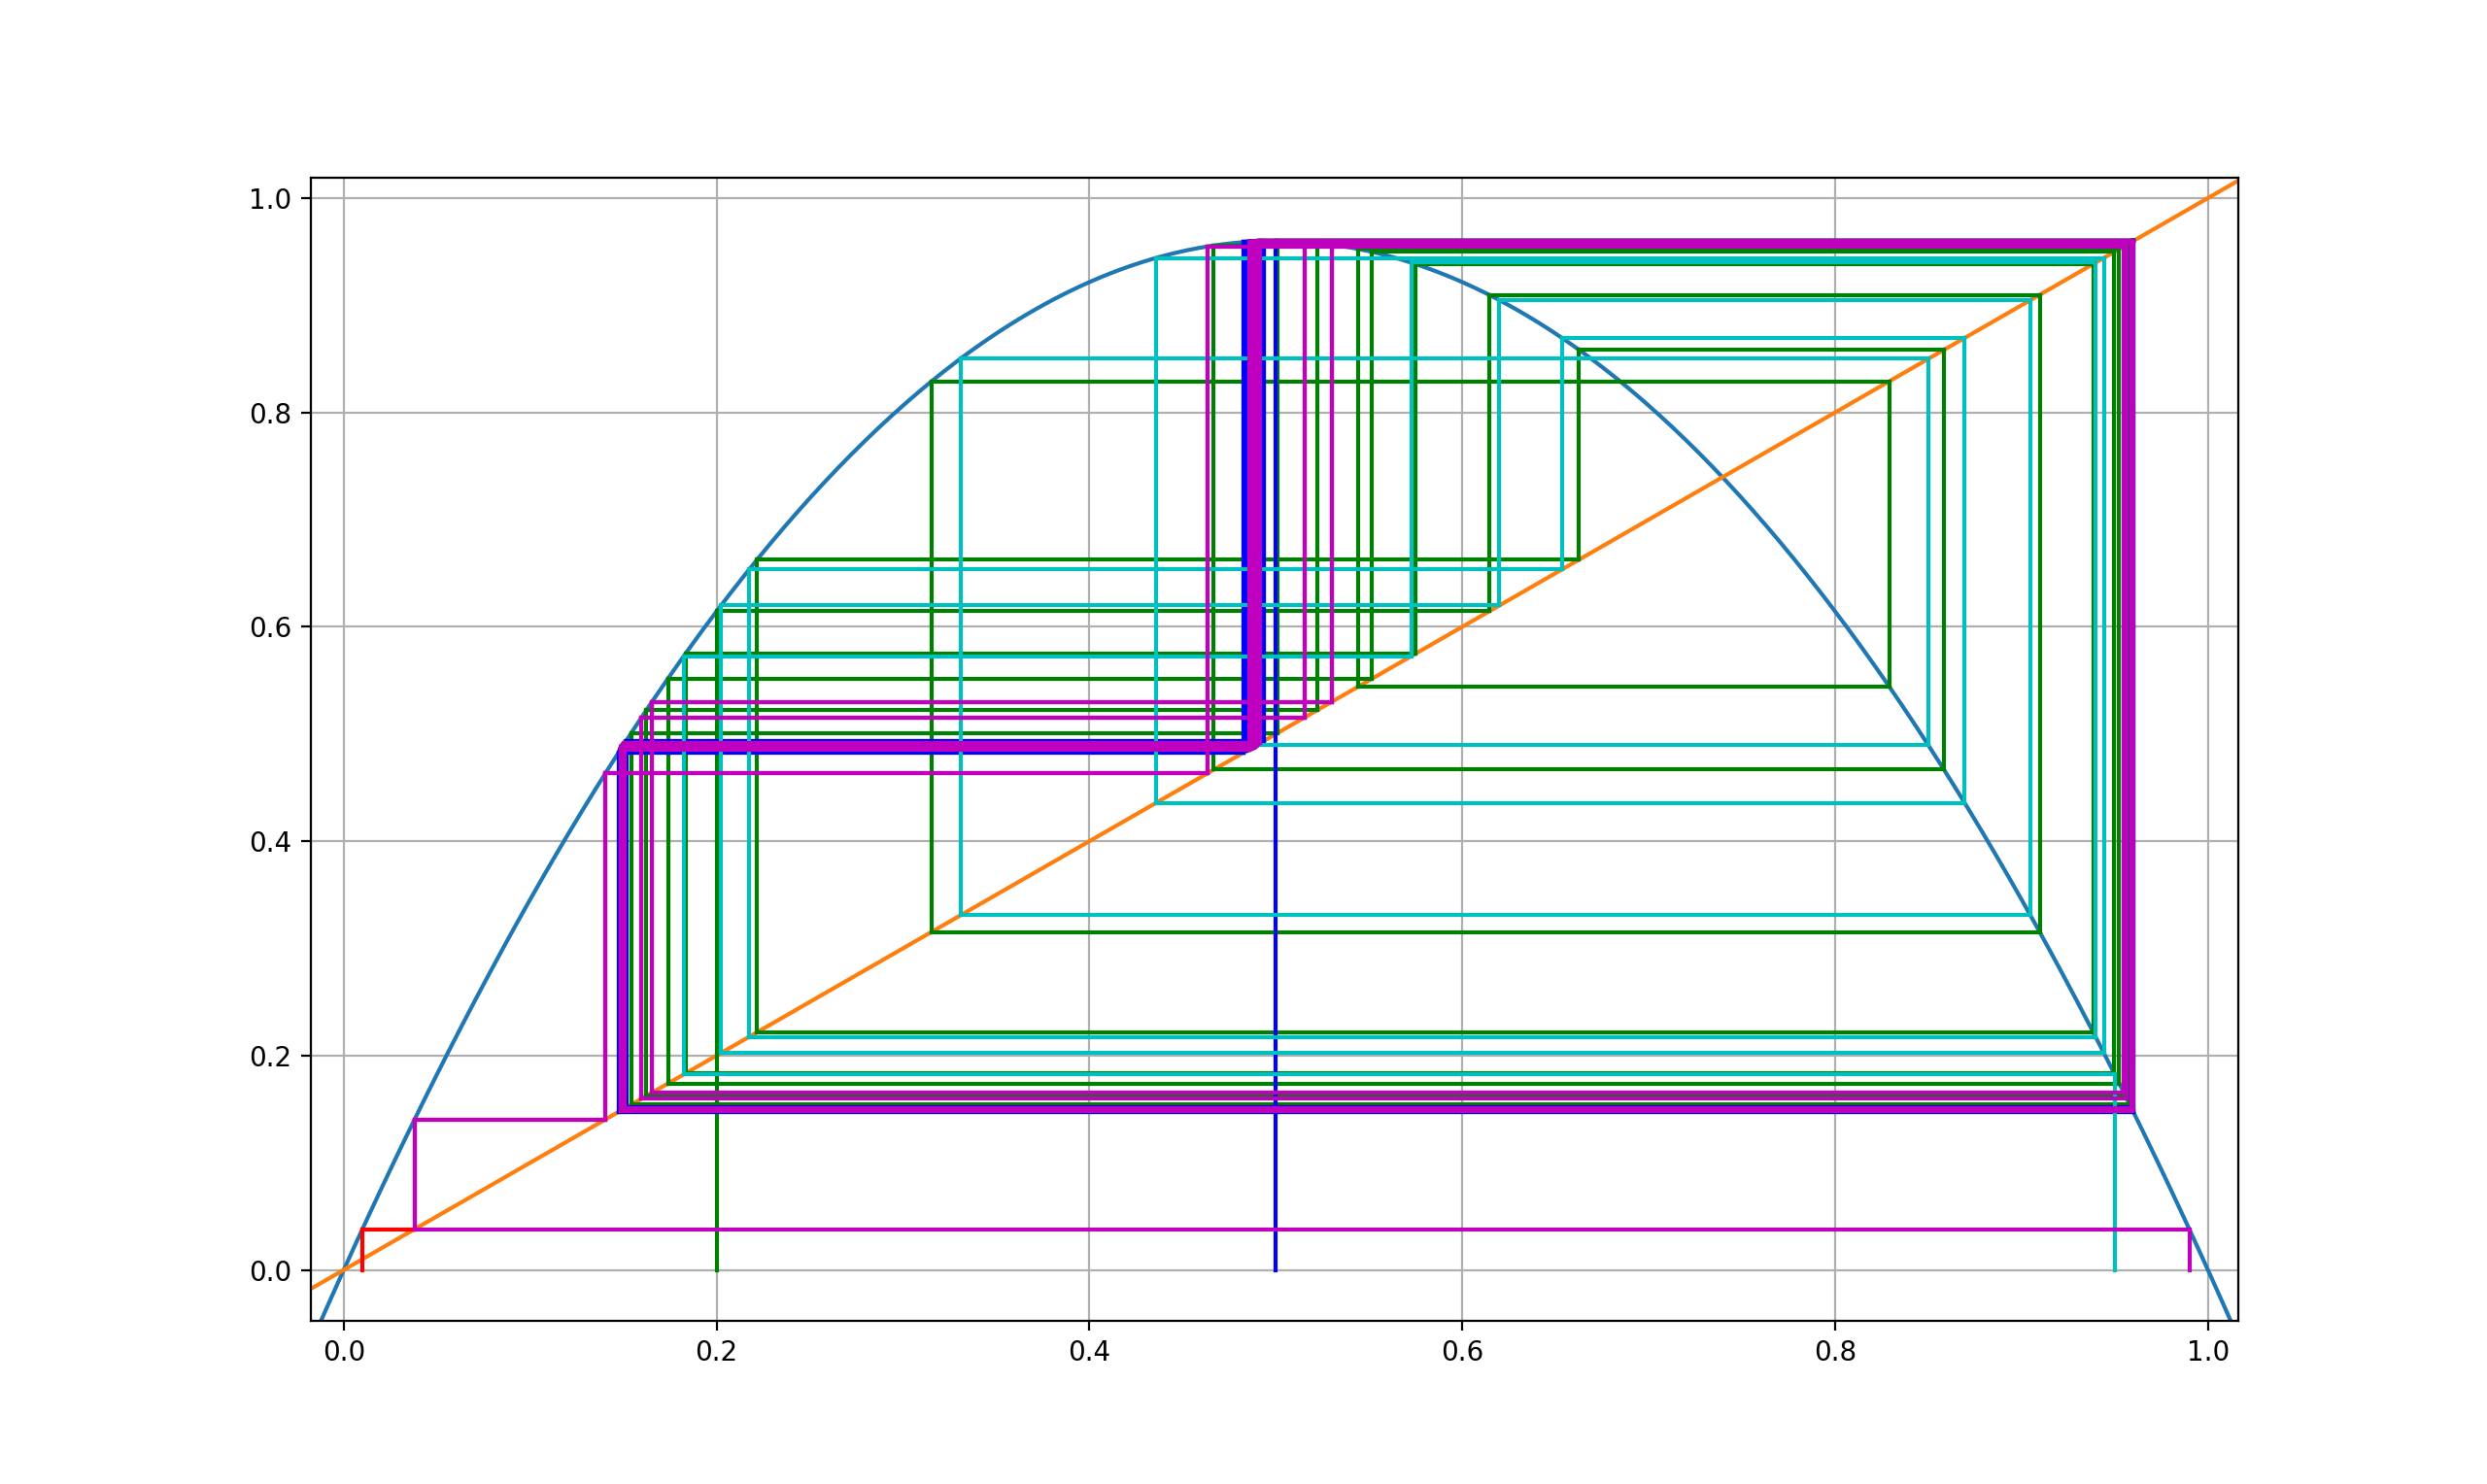
\includegraphics[width=0.9\textwidth]{figure/section1/logistic384.png} \\
\end{minipage}
\caption{Periodic-3 window and cobweb plot in $a = 3.84$}\label{logistic-cobweb-plot1}
\end{figure}

That's fine, let's check the result by cobweb plot. Ok, hold on a second, something wrong! So we still need more analysis.

Obviously, every periodic-3 orbit of $g$ is a fixed point of $g^3$, so we can also analysis $g^3$ map.\\[3ex]

\begin{figure}[H]
\begin{minipage}[c][0.33\width]{0.33\textwidth}
   \centering
   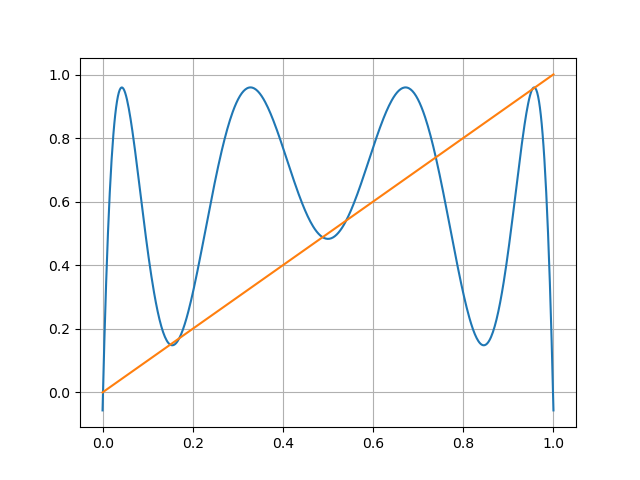
\includegraphics[width=\textwidth]{figure/section1/g3logistic-origin.png}
\end{minipage}
\begin{minipage}[c][0.33\width]{0.33\textwidth}
   \centering
   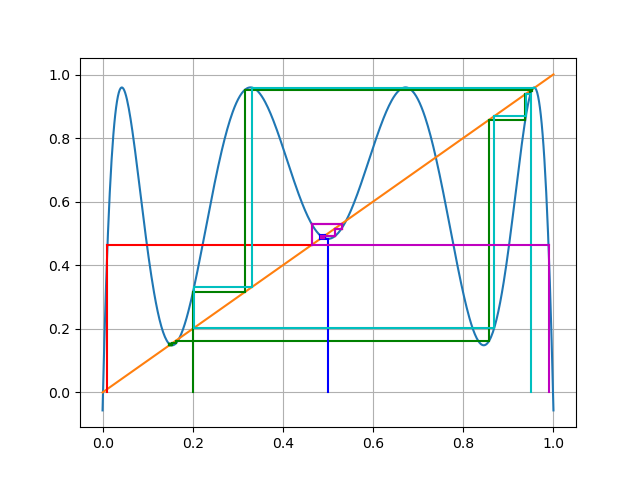
\includegraphics[width=\textwidth]{figure/section1/g3logistic384.png}
\end{minipage}
\begin{minipage}[c][0.33\width]{0.33\textwidth}
   \centering
   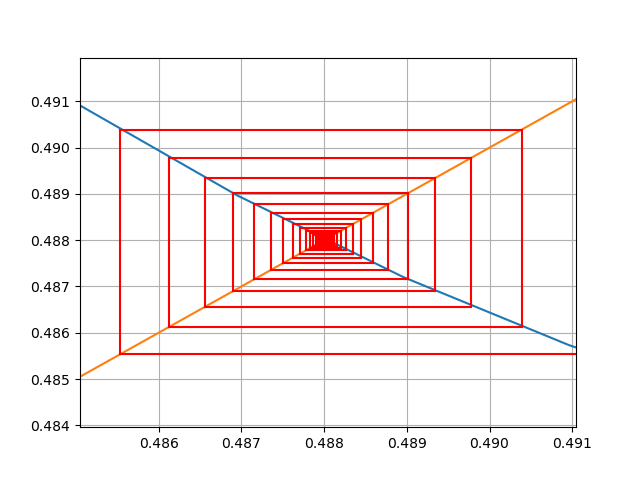
\includegraphics[width=\textwidth]{figure/section1/g3logistic384-001-detail.png} 
\end{minipage}
\\[3ex]\caption{$g^3$ map and $g^3$ cobweb plot figure}\label{logistic-cobweb-plot1}
\end{figure}

We found different from periodic-2 orbit, the periodic-3 orbit is nearby(rather than equal) the point and it seems we have periodic-3 orbit. Actually, we will explain all periodic-3 will implies a characteristic we called ``chaos''. 






\newpage
  \noindent \textbf{[ii] The Logistic Map $G(x) = 4x(1-x)$}
\\\noindent Now we consider another logistic map where $a \equiv 4$. \\[1ex]
\\\noindent Firstly, why we are interested in $g_4(x)$, consider a quadratic function 
$$
g_a(x) = ax(1-x) = a(-x^2 + x - 1 + 1) = -a(x-{1\over 2})^2 +{a\over 4}
$$
this function have maximum at point $x = 1/2$ and the maximum is $a/4$. As we have the Theo. \ref{sink-source-point}, if we consider the sink point set, it is necessary to satisfy $|g_a(x)| < 1$, or${a \over } 4 < 1 \Rightarrow a < 4$. So at the point $a = 4$, this set is empty and this is a critical state. For every $a_{new} = a - \varepsilon (\varepsilon \rightarrow 0)$, we have the interval of sink. So at this point, some special property has been result and that is why we interested in this map.

We can still find the fixed point of $g_4(x)$ to solve $g_4(x) = x$, and we have $x_{11} = 0, x_{21} = {3/4}$. If we consider periodic-k orbit, for instance, we consider periodic-2 orbit, then we have solve the function $g(g(x)) = x$ as 
$$
g(g(x)) = 4(4x(1-x))[1-4x(1-x)] = x \Rightarrow (4x^2-4x+1)(x-1)x+{x\over 16} = 0 
$$
$$
\Rightarrow (4x-3)(16x^2 - 20x+5)x = 0 \Rightarrow x_{21} = 0, x_{22} = {3\over 4}, x_{23,24} = {5\pm \sqrt{5}\over 8}
$$

Also, it is easy to check the periodic-k orbit in the figure.\\[2ex]

\begin{figure}[H]
\begin{minipage}[c][0.24\width]{0.24\textwidth}
   \centering
   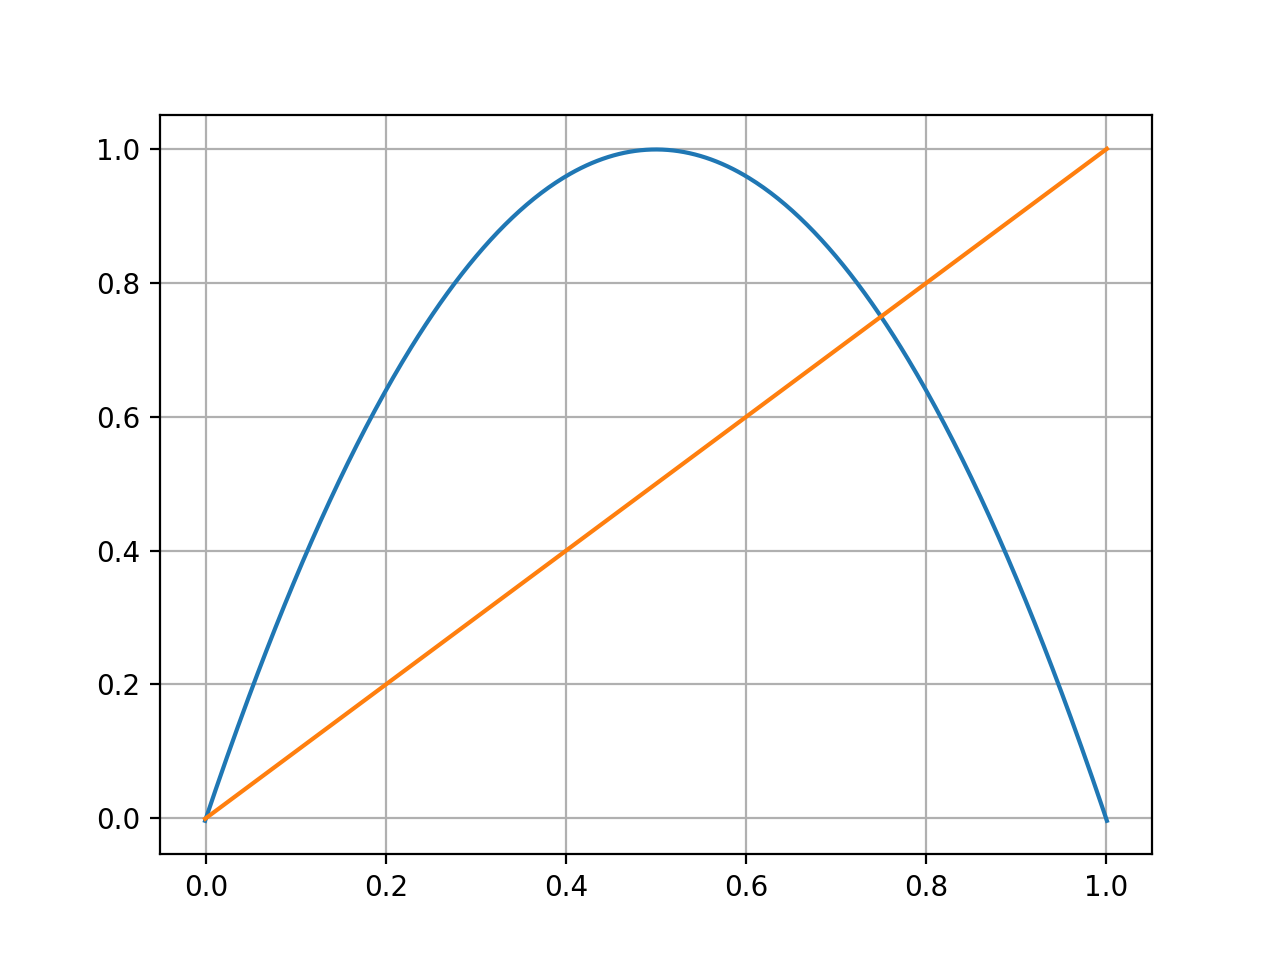
\includegraphics[width=\textwidth]{figure/section1/4-logistic-ite-1.png}
\end{minipage}
\begin{minipage}[c][0.24\width]{0.24\textwidth}
   \centering
   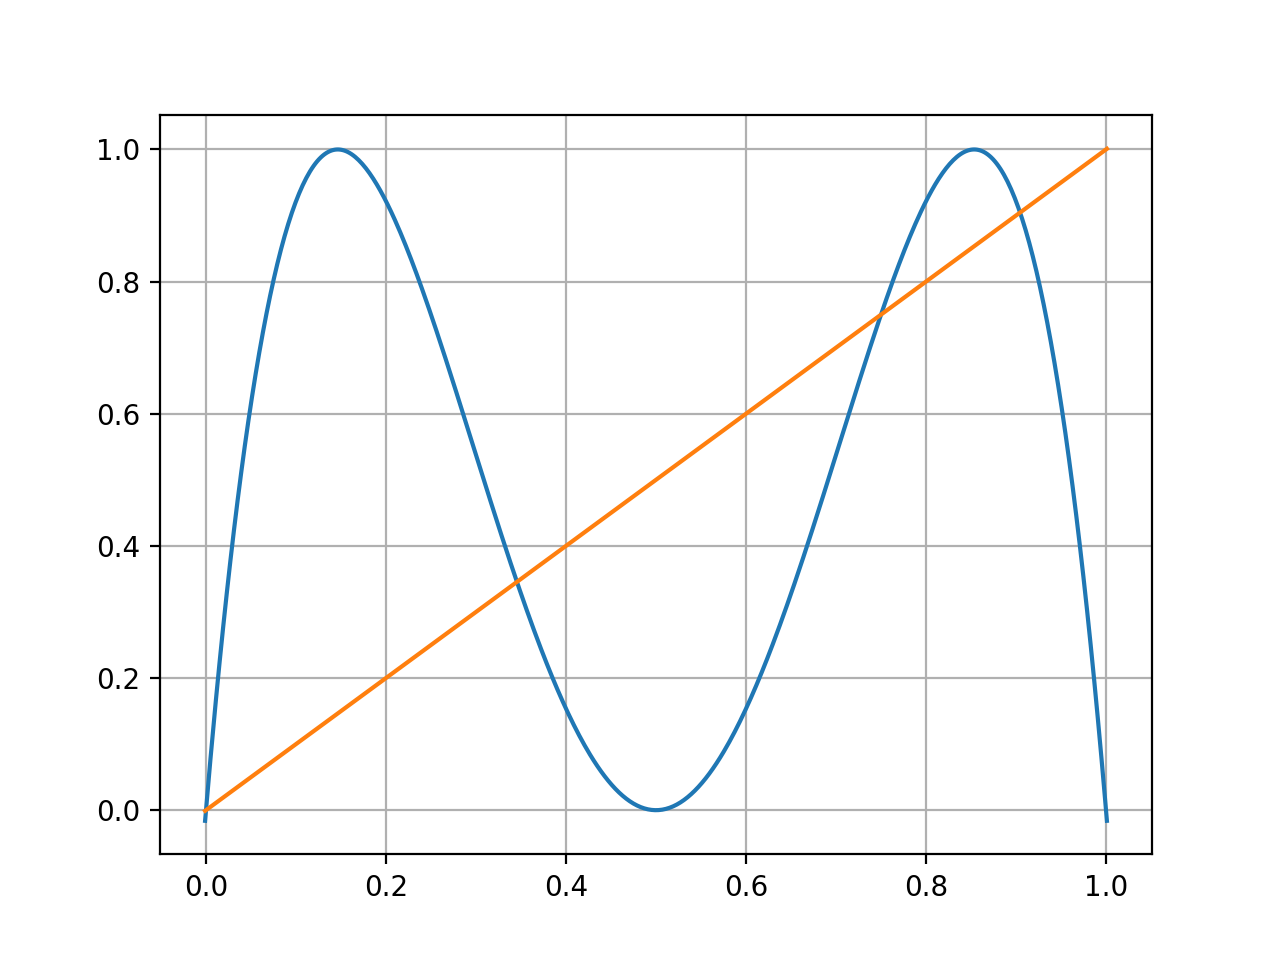
\includegraphics[width=\textwidth]{figure/section1/4-logistic-ite-2.png}
\end{minipage}
\begin{minipage}[c][0.24\width]{0.24\textwidth}
   \centering
   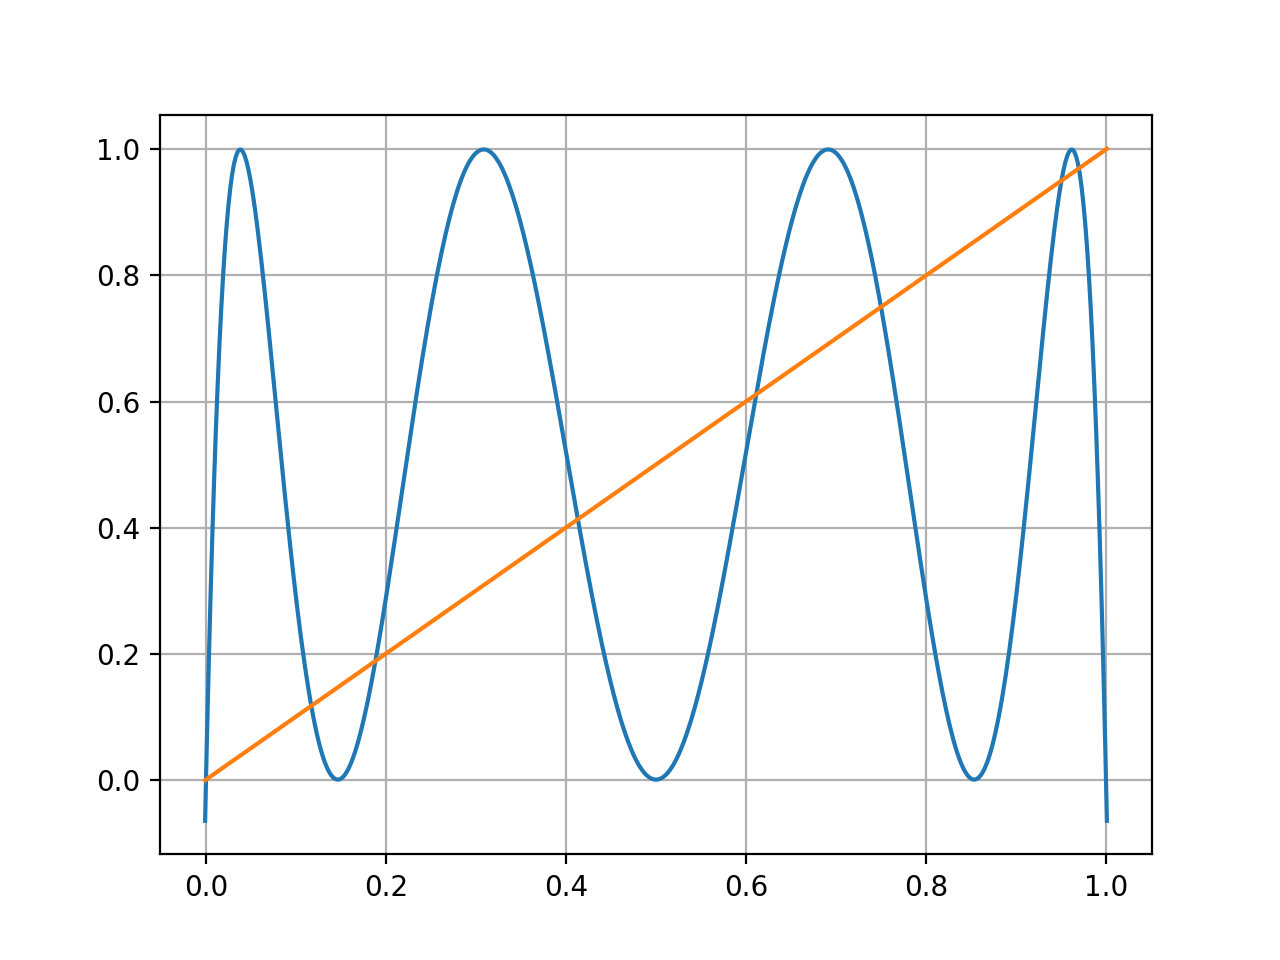
\includegraphics[width=\textwidth]{figure/section1/4-logistic-ite-3.png}
\end{minipage}
\begin{minipage}[c][0.24\width]{0.24\textwidth}
   \centering
   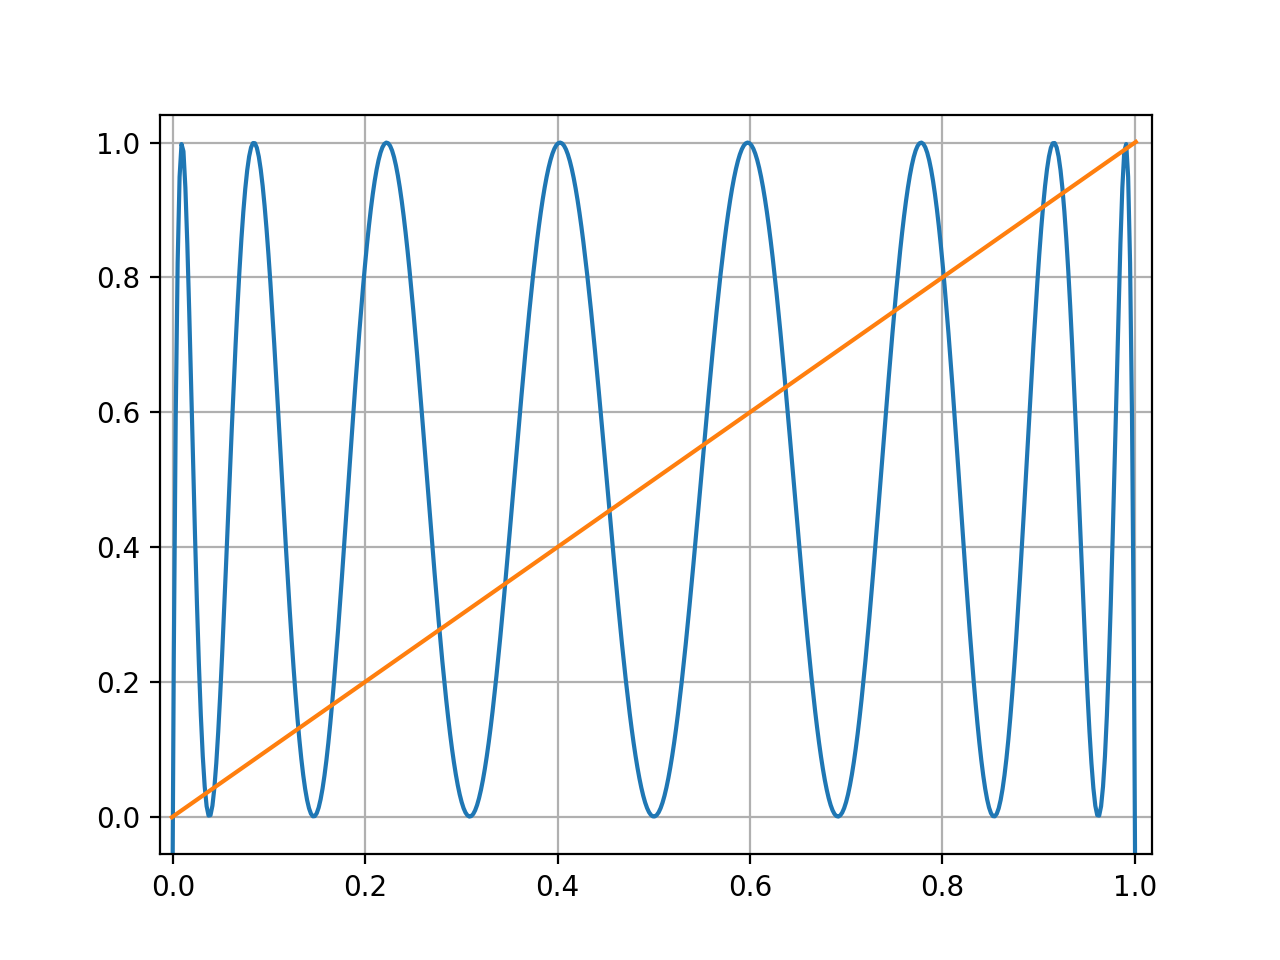
\includegraphics[width=\textwidth]{figure/section1/4-logistic-ite-4.png}
\end{minipage}
\\[3ex]\caption{$g_4^1, g_4^2, g_4^3$ and $g_4^4$ figure}\label{4-logistic-ite}
\end{figure}

\begin{figure}[H]
\begin{center}
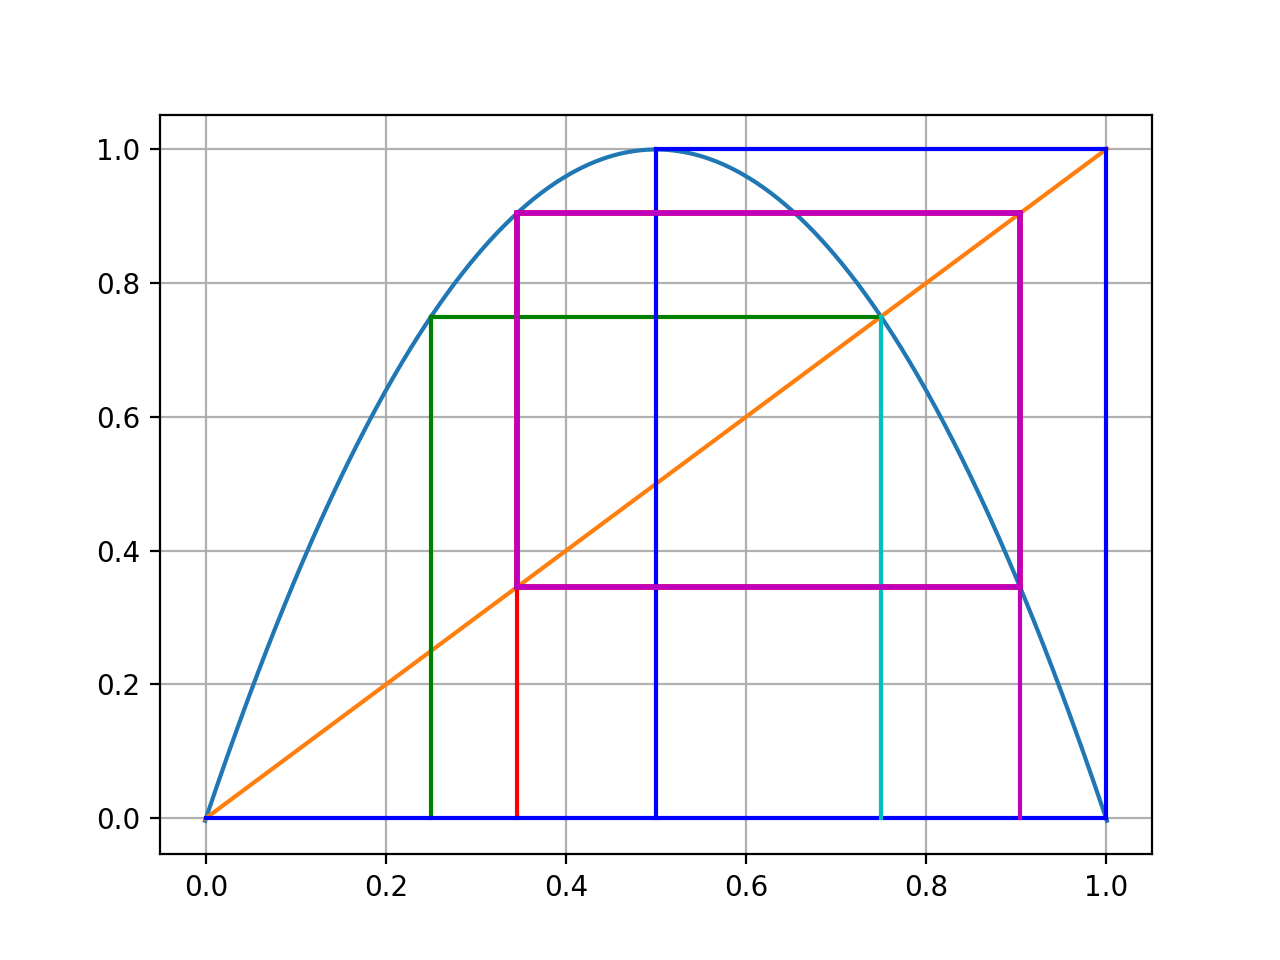
\includegraphics[width=0.5\textwidth]{figure/section1/4-logistic-cobweb-plot.png}\\
\caption{$g_4(x)$ cobweb plot(periodic-1,2 orbits)}\label{4-logistic-ite}
\end{center}
\end{figure}

\newpage
We found a conclusion here
\begin{conclusion}
For every periodic-k, the model $g_4^k$ have $2^{k} - 1$ saddle-node bifurcation and $2^k$ fixed point. And these $2^k$ points include every fixed point for model $g_4^{i}, i = 1, 2, \ldots, k-1 \land k \equiv 0 (\text{mod } i)$
\end{conclusion}

The number of orbits of the map for each period can be tabulated in the map's periodic table.



\begin{table}[H]
\centering  
\caption{The periodic table for the logistic4 map}  
\begin{tabular}{|c||c|c|c|c|c|c|c|}
\hline
Period $k$                             & 1 & 2 & 3 & 4  & 5  & 6  & 7   \\
\hline
\hline
Number of fixed points of $g_4^k$      & 2 & 4 & 8 & 16 & 32 & 64 & 128 \\
\hline
Orbits of Period $k$                   & 2 & 1 & 2 & 3  & 4  & 5  & 6   \\
\hline
Fixed points due to lower orbits       & 0 & 2 & 2 & 4  & 2  & 4  & 2   \\
\hline
\hline
1                                      & / &   &   &    &    &    &   \\
2                                      & * & / &   &    &    &    &   \\
3                                      & * &   & / &    &    &    &   \\
4                                      & - & * &   & /  &    &    &   \\
5                                      & * &   &   &    & /  &    &   \\
6                                      & - & * & * &    &    & /  &   \\
7                                      & * &   &   &    &    &    & / \\
\hline
\end{tabular}  
\end{table}
(*: Greatest common divisor group, -: $g^k$ fixed)
\end{discussion}







\subsection{Chaos}
We still focus on $g_4(x)$ map, we try to check the $g_4^2$ fixed point ${5 - \sqrt{5}\over 8}$.\\[2ex]

\begin{figure}[H]
\begin{minipage}[c][0.24\width]{0.24\textwidth}
   \centering
   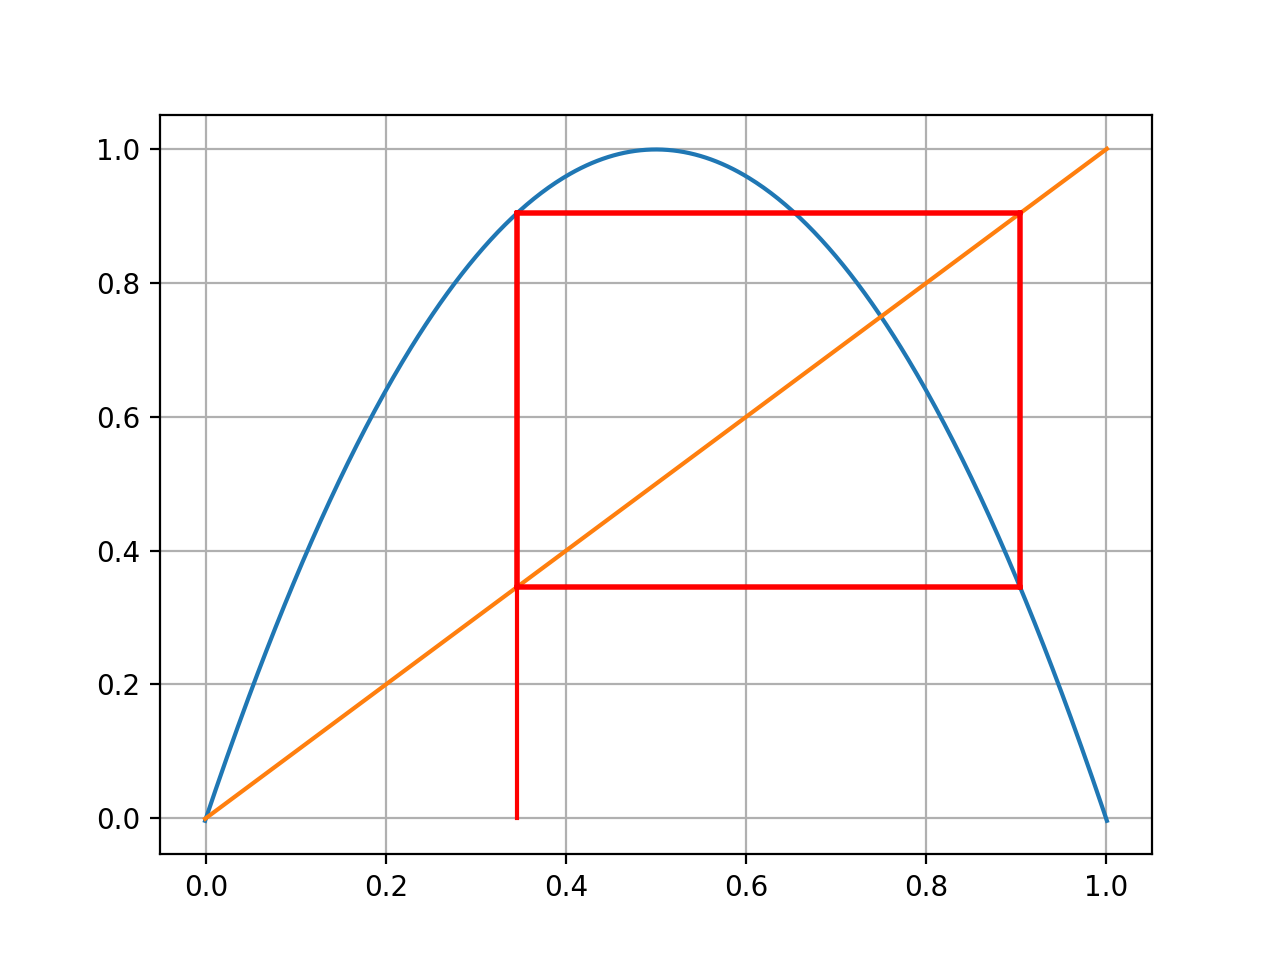
\includegraphics[width=\textwidth]{figure/section1/4-logistic-stable-30.png}
\end{minipage}
\begin{minipage}[c][0.24\width]{0.24\textwidth}
   \centering
   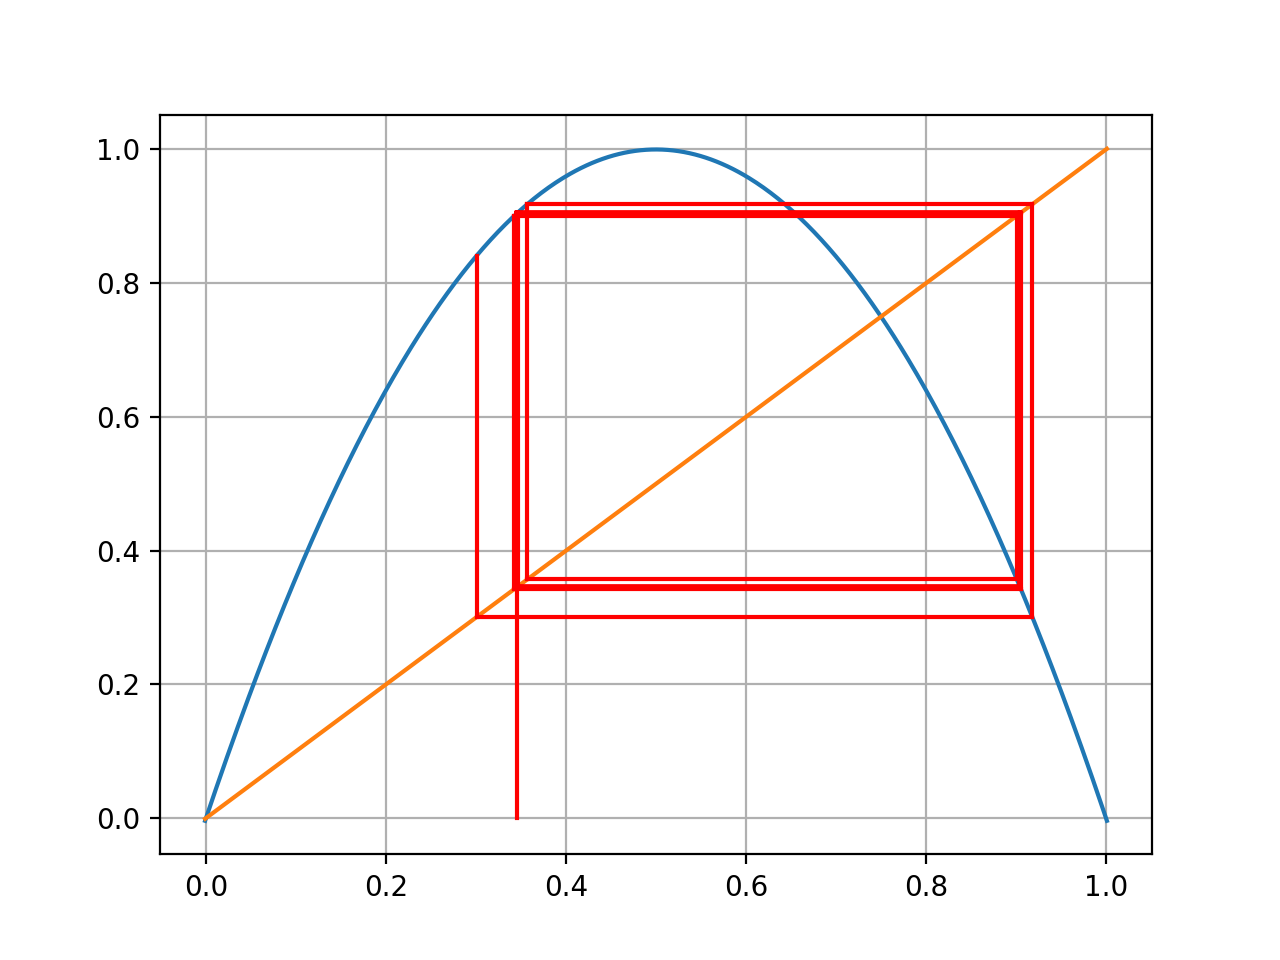
\includegraphics[width=\textwidth]{figure/section1/4-logistic-stable-50.png}
\end{minipage}
\begin{minipage}[c][0.24\width]{0.24\textwidth}
   \centering
   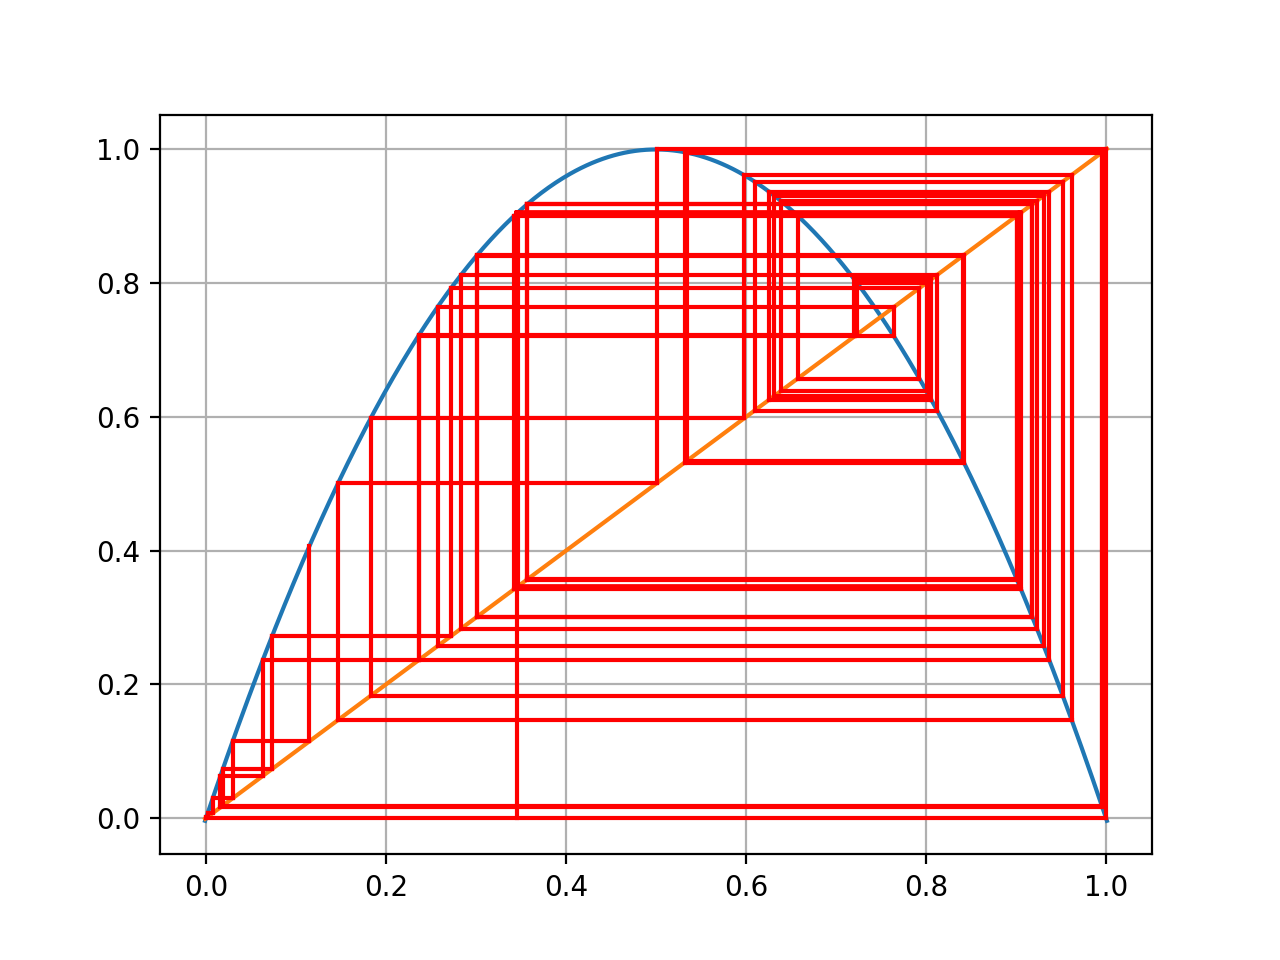
\includegraphics[width=\textwidth]{figure/section1/4-logistic-stable-100.png}
\end{minipage}
\begin{minipage}[c][0.24\width]{0.24\textwidth}
   \centering
   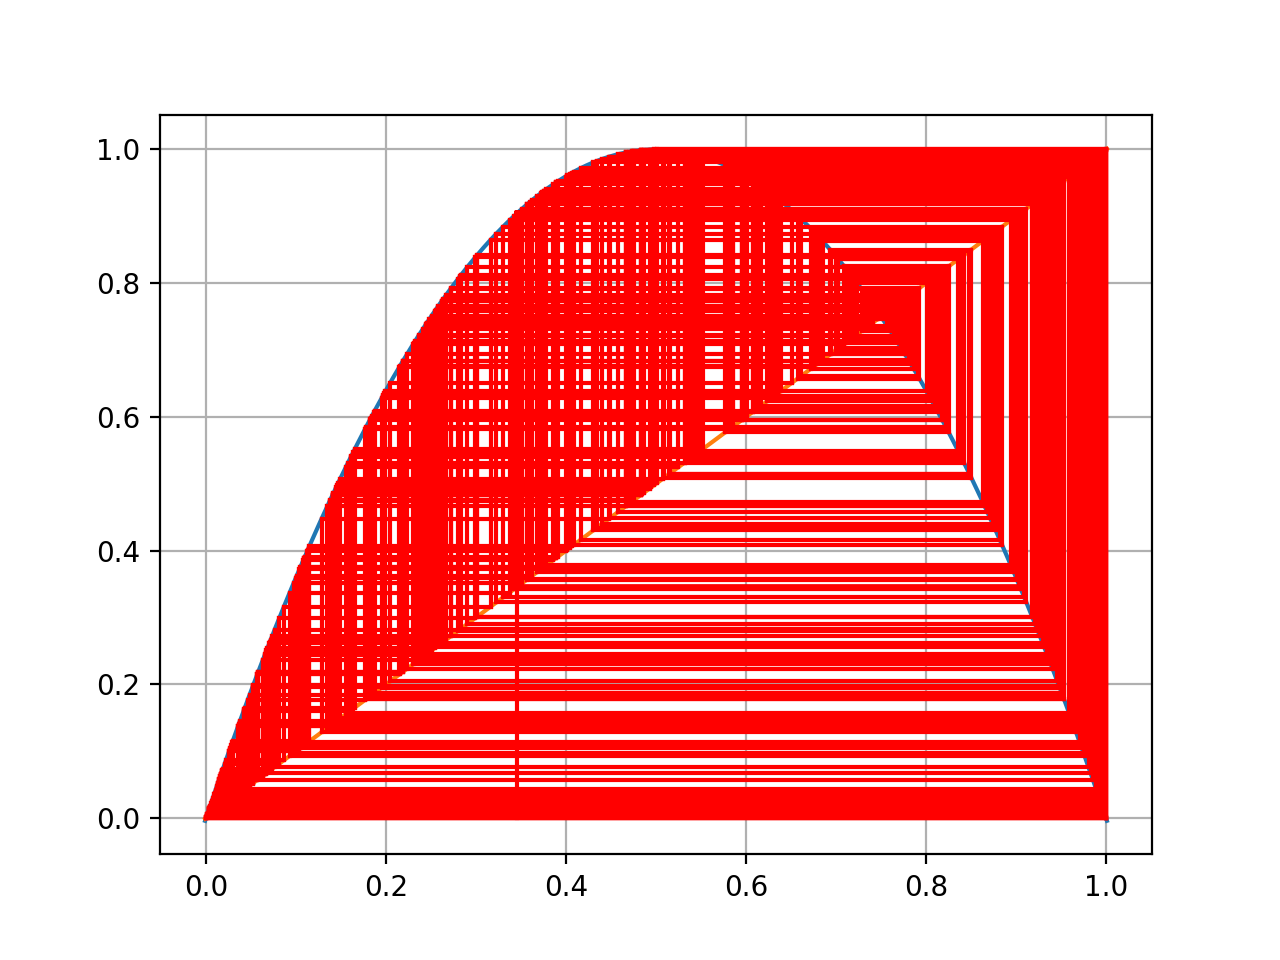
\includegraphics[width=\textwidth]{figure/section1/4-logistic-stable-500.png}
\end{minipage}
\\[3ex]\caption{$g_4^1, g_4^2, g_4^3$ and $g_4^4$ figure}\label{4-logistic-ite}
\end{figure}

It seems something wrong. Because we proved that ${5 \pm \sqrt{5}\over 8}$ is a periodic orbit during the iteration, but once we growth the iteration times, the results filled all the interval.

So what happened? We try to put all of our data into a same image, and we have
\begin{figure}[H]
\begin{center}
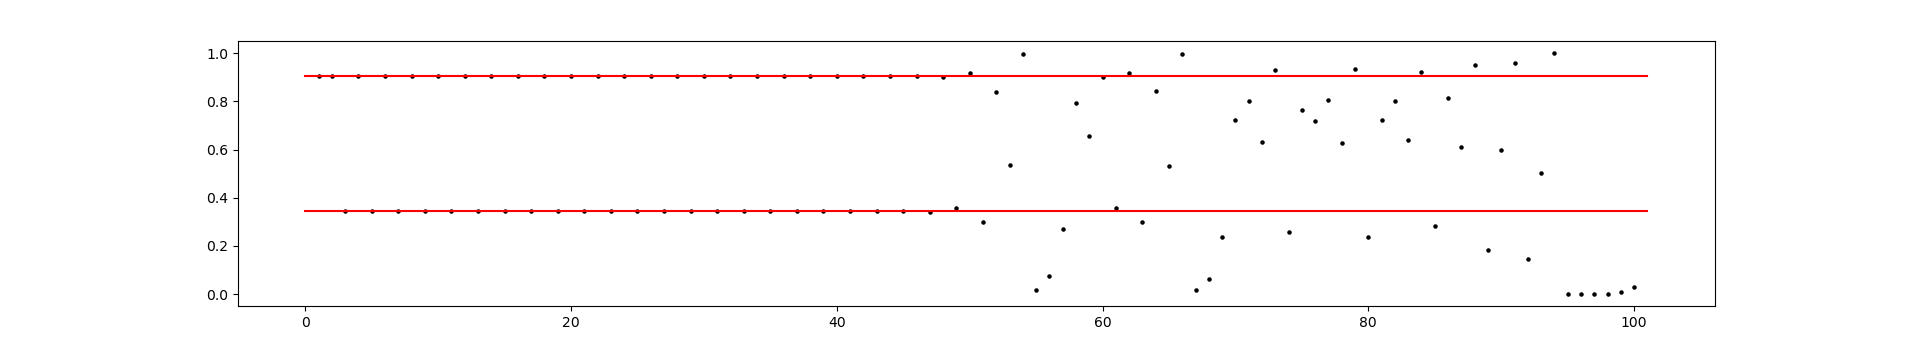
\includegraphics[width=0.8\textwidth]{figure/section1/4-logistic-stable-check.png} \\
\caption{Iteration and ``periodic-2 orbit'' value}\label{periodic-2-check}
\end{center}
\end{figure}

Obviously, in about first 40 times iteration, it was worked for a while, but with the iteration increasing, the error also increaed rapidly. Ok, ok, let's check the data for more details.
\begin{table}[H]
\centering  
\caption{Logistic4 periodic-2 orbit iteration}  
\begin{tabular}{|c||c|c|c|c|}
\hline
1-4   & 0.3454915028125262  & 0.9045084971874737  & 0.3454915028125262  & 0.9045084971874735 \\
\hline
5-8   & 0.34549150281252694 & 0.9045084971874745  & 0.3454915028125237  & 0.9045084971874705 \\
\hline
9-12  & 0.34549150281253665 & 0.9045084971874865  & 0.3454915028124849  & 0.9045084971874225 \\
\hline
13-16 & 0.34549150281269186 & 0.9045084971876783  & 0.3454915028118641  & 0.9045084971866552 \\
\hline
17-20 & 0.3454915028151752  & 0.9045084971907479  & 0.34549150280193086 & 0.9045084971743771 \\
\hline
21-24 & 0.3454915028549078  & 0.9045084972398602  & 0.3454915026430002  & 0.904508496977928  \\
\hline
25-27 & 0.3454915034906304  & 0.9045084980256565  & 0.34549150010010987 & $\ldots$           \\
\hline
\end{tabular}  
\end{table}

We noticed that during the iteration, the values of periodic-2 orbit are actually changed very small. Then we realized that is beacause of ${5 - \sqrt{5}\over 8} \neq 0.3454915028125262$ and this is just a value near the periodic point.(And the computer can only calculate this estimation value rather than real value.) Even this two value are almost nearby, it still have a little difference, and this difference become larger and larger during the iteration.

That is important beacause we found even two value are almost equal, after iterate, this tiny, tiny difference will become a catastrophe and eventually two orbits move apart.

\begin{definition}\textbf{Sensitive dependence on initial conditions, Sensitive point}
\\\noindent Let $f$ is a map on $R$, $x_0$ in domain.
\\\noindent If there is a nonzero distance $d$ s.t. some points arbitrary near $x_0$ are eventually mapped at least $d$ units from the corresponding image of $x_0$, then we called $x_0$ has \textbf{sensitive dependence on initial conditions};
\\\noindent If for this $x_0, \exists \varepsilon > 0$ s.t. $\forall x \in N_\varepsilon^o(x_0) = N_\varepsilon(x_0) \backslash \{x_0\}, \exists K$ s.t. $\forall k > K, ||f^k(x) - f^k(x_0)|| \geq \varepsilon$, then called this point is \textbf{sensitive point}.
\end{definition}
\begin{definition}\textbf{Eventually periodic}
\\\noindent Let $f$ is a map on $R$, $x_0$ in domain. If for some positive integer $N, \forall n > N, f^{n+p}(x) = f^n(x)$, then we called $x$ \textbf{eventually periodic} with period p, where p is the smallest such positive integer.
\end{definition}

Now we consider another model to explain this definition in another way.

\begin{example}Consider a map $f(x) = 3x (\text{mod } 1)$. (e.g. $f(4.33) = 0.33, f(-1.98) = 0.02$.)
\end{example}

\begin{figure}[H]
\begin{center}
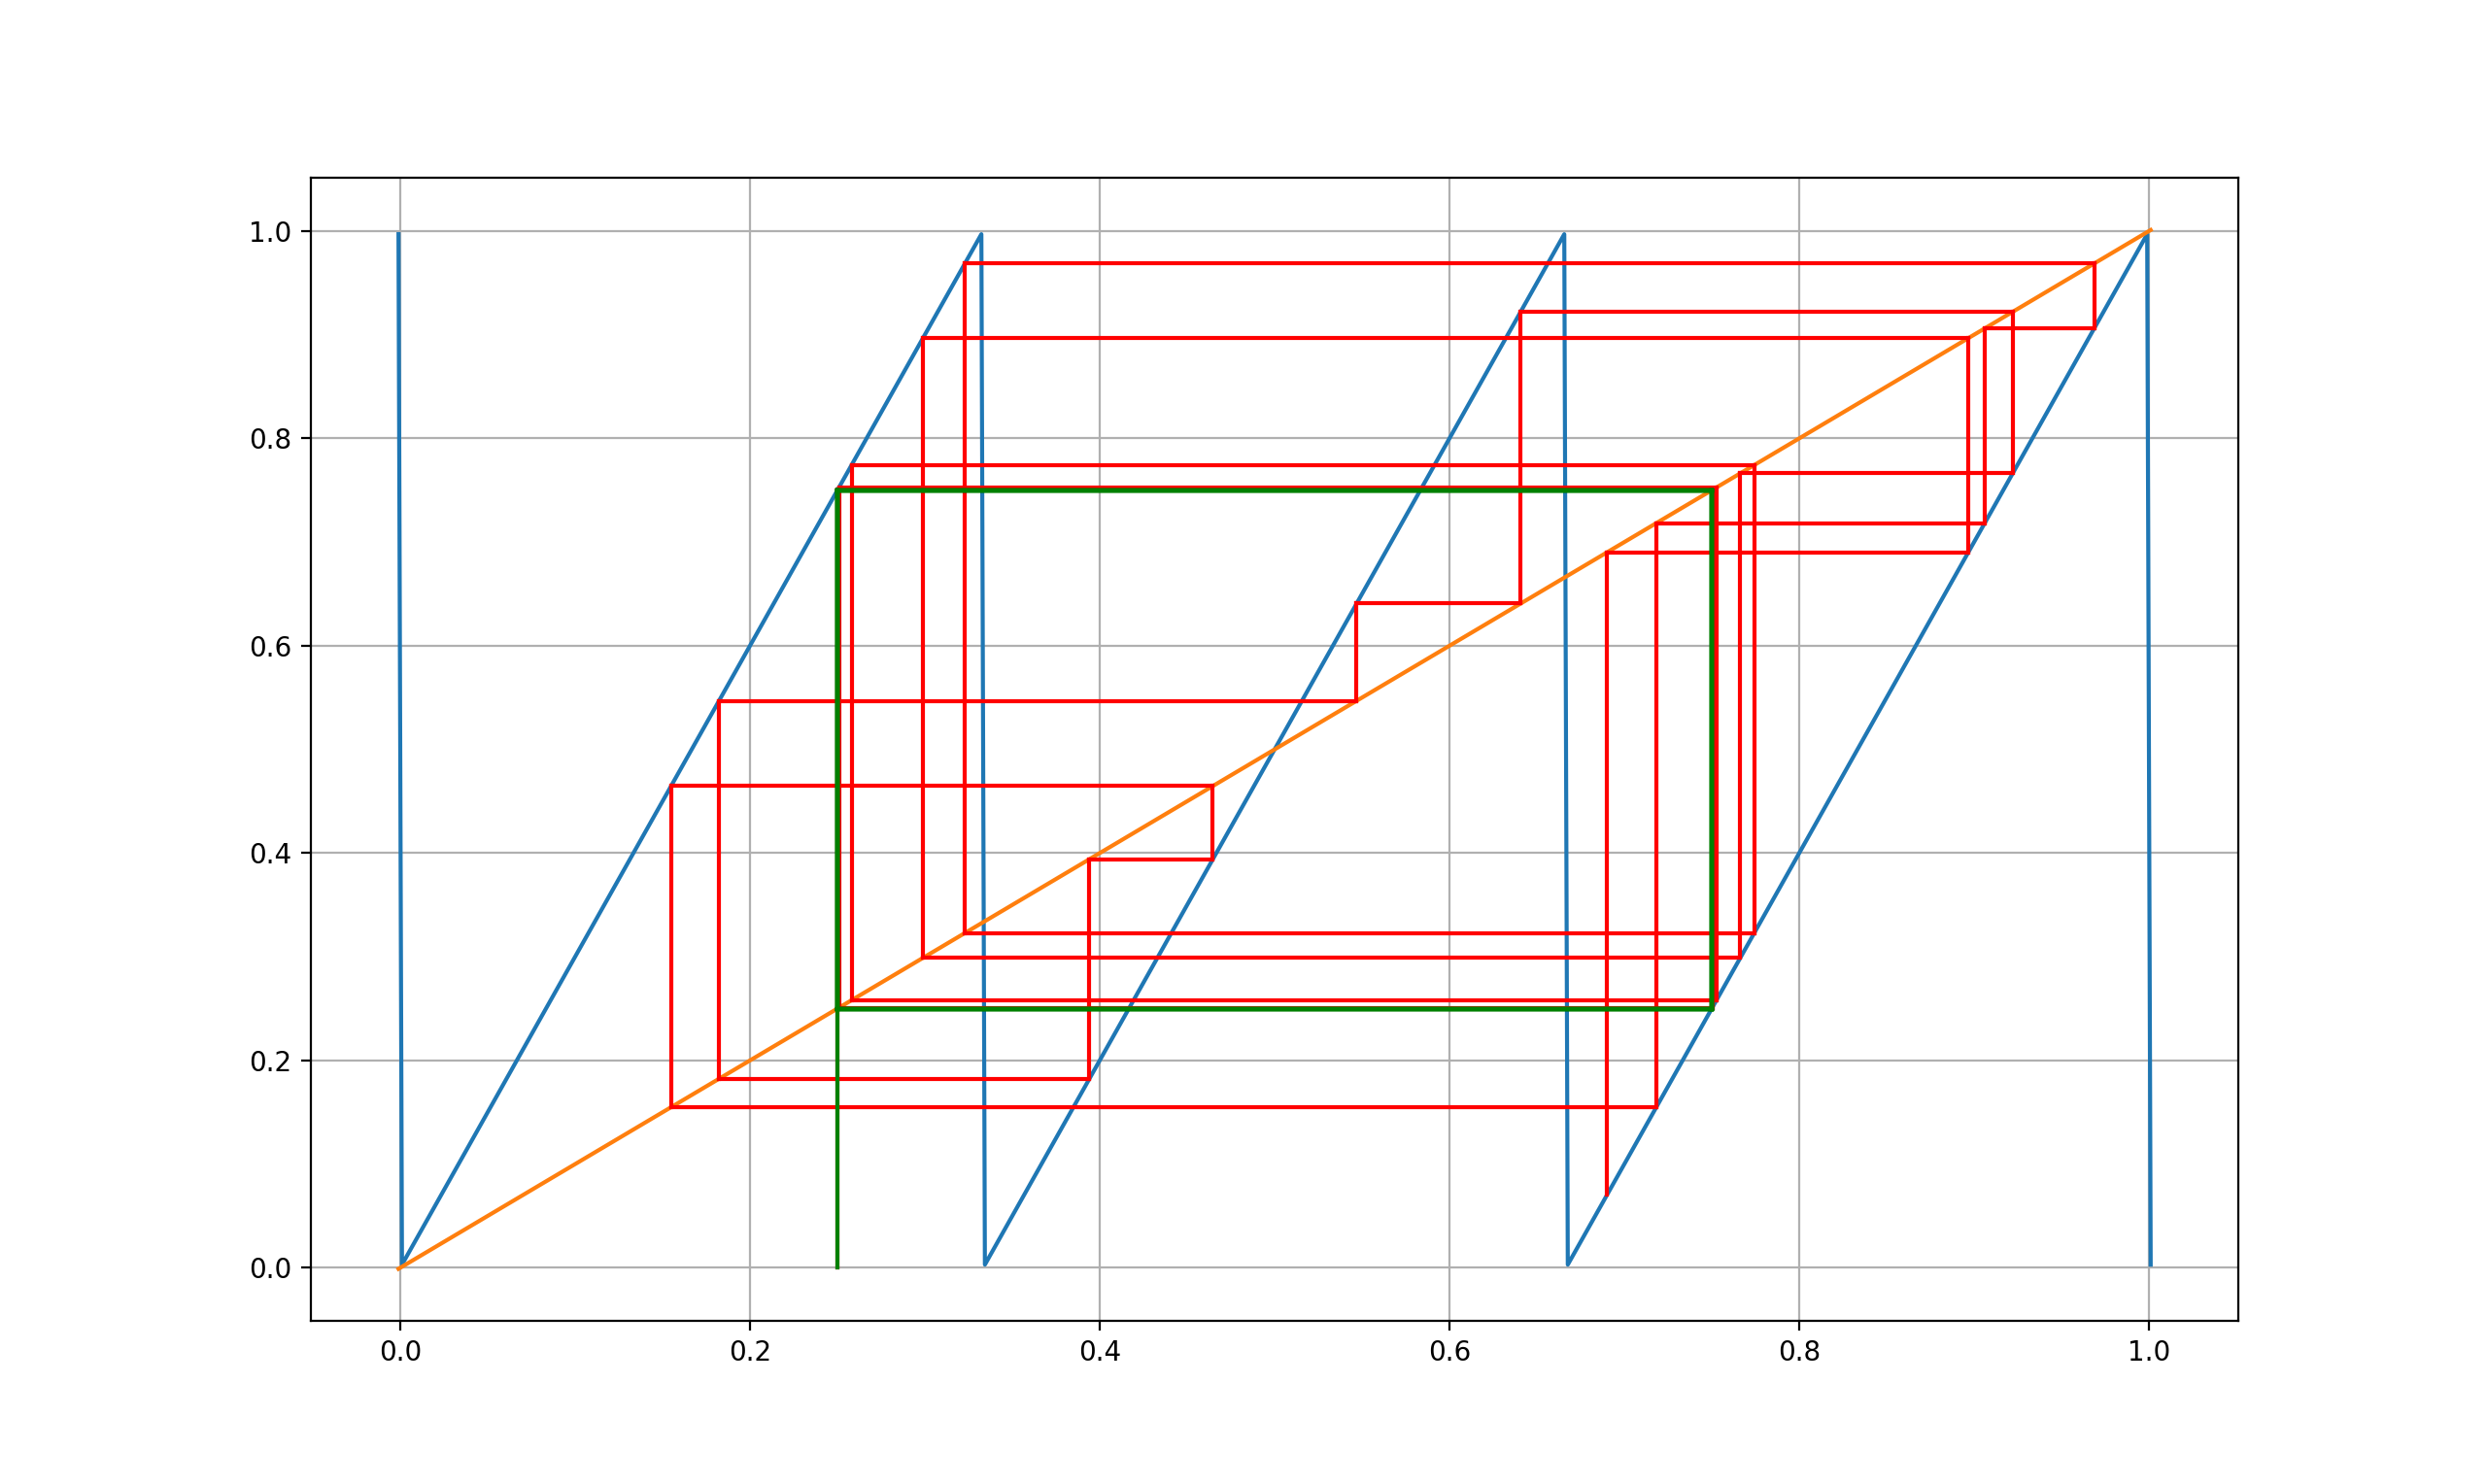
\includegraphics[width=0.4\textwidth]{figure/section1/3xmod1.png} \\
\caption{3x mod 1 cobweb plot(initial value: {\color{green}0.25(green)}, {\color{red}0.2501(red)})}\label{3xmod1}
\end{center}
\end{figure}

\newpage
Basically, we have
\begin{theorem} For any map $f$, the source has sensitive dependence on initial conditions.
\end{theorem}
{\color{blue}
\begin{proof} For a certain $\varepsilon$, as $p$ is a source, then $\forall x \in N^o_\varepsilon(p), \lim_{k \rightarrow \infty}f^k(x) \notin N^\varepsilon_d(p) \Rightarrow d(p, x) > \varepsilon$ $\blacksquare$   
\end{proof}
}

Is there any way to investigate this sensitive dependence? Yes, and here we will introduce a method called \textbf{itinerary} of an orbit.

{\color{blue}
\begin{solution}\textbf{Itinerary}
\\\noindent We still consider the $g_4$ model. Assign the symbol \textbf{L} to the left subinterval $[0, 1/2]$ and \textbf{R} to the right subinterval $[1/2, 1]$. Then, for every initival condition $x_0$, we can list the itinerary with \textbf{L} and \textbf{R}. 
\\\noindent For instance, the initial point $x_0 = 1/3$ have the itinerary \textbf{LRLRLRRLLRR}
\begin{table}[H]
\centering  
\caption{Logistic4 $1/3$ itinerary}  
\begin{tabular}{|c||c|c|c|}
\hline
0-2   & 0.333333333333333  (\textbf{L}) & 0.888888888888889  (\textbf{R})  & 0.39506172839506154 (\textbf{L}) \\
\hline
3-5   & 0.9559518366102727 (\textbf{R}) & 0.16843169076687667(\textbf{L})  & 0.5602498252491516 (\textbf{R})  \\
\hline
6-8   & 0.9854798342297868 (\textbf{R}) & 0.05723732222487492 (\textbf{L}) & 0.21584484467760304(\textbf{L})  \\
\hline
9-10  & 0.6770233908148179 (\textbf{R}) & 0.874650876417697   (\textbf{R}) & $\ldots$                         \\
\hline
\end{tabular}  
\end{table}

And we can list all itinerary with different initial value.$\blacksquare$
\begin{table}[H]
\centering  
\caption{Logistic4 itinerary with different initial value}  
\begin{tabular}{|c||l|l|l|l|l|}
\hline
Val  & $1-10$              & $11-20$             & $21-30$             & $31-40$             & $\ldots$ \\
\hline
\hline
0.01 & \textbf{LLLRRLLLLR} & \textbf{RRRLRLRLRR} & \textbf{LLRRRLLRRR} & \textbf{RLRRLRLRLR} & $\ldots$ \\
\hline
0.25 & \textbf{LRRRRRRRRR} & \textbf{RRRRRRRRRR} & \textbf{RRRRRRRRRR} & \textbf{RRRRRRRRRR} & $\ldots$ \\
\hline
1/3  & \textbf{LRLRLRRLLR} & \textbf{RLRLLRRRRL} & \textbf{LLLRRRRLRL} & \textbf{RRRRRRRLRR} & $\ldots$ \\
\hline
0.5  & \textbf{RRLLLLLLLL} & \textbf{LLLLLLLLLL} & \textbf{LLLLLLLLLL} & \textbf{LLLLLLLLLL} & $\ldots$ \\
\hline
1    & \textbf{RLLLLLLLLL} & \textbf{LLLLLLLLLL} & \textbf{LLLLLLLLLL} & \textbf{LLLLLLLLLL} & $\ldots$ \\
\hline
\end{tabular}  
\end{table}

\end{solution}
}




Notice that there are some conclusions.
\begin{conclusion} For every periodic-k point, the itinerary of orbit will repeats \textbf{L} or \textbf{R} infinitely.
\end{conclusion}

\begin{conclusion} For every $k$ iterate, the itinerary have $2^k$ choice and the sum of their lengths is 1(or the length of the interval).
\end{conclusion}

Also, we have a conclusion not very obvious.

\begin{conclusion} Each $2^k$ itinerary is shorter than $\pi / 2^{k+1}$.
\end{conclusion}
We will prove this conclusion in later sections.



\newpage
We can also analysis the problem with \textbf{transition graph}.

\begin{figure}[H]
\begin{center}
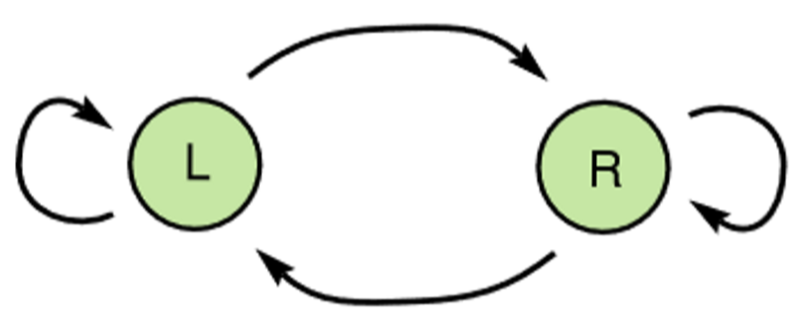
\includegraphics[width=0.2\textwidth]{figure/section1/transition-graph-1.png} \\
\caption{Transition graph}\label{transition-graph-1}
\end{center}
\end{figure}

Finally, we focus on the title of this subsection ``chaos'', after these analysis, it is simple to summary the definition of chaos.

\begin{definition}\label{chaos-orbit}\textbf{Chaos}
\\\noindent A chaotic orbit is a bounded, non-periodic orbit that displays sensitive dependence. Chaotic orbits seoarate exponentially fast from their neighbors as the map iterated.
\end{definition}


\begin{theorem} \label{p3-chaos}The existence of periodic-3 orbit alone implies the existence of a large set of sensitive points, or chaotic orbit.
\end{theorem}

We will prove this problem in appendix.

\newpage

%~~~~~~~~~~~~~~~~~~~~~~~~~~~~~~~~~~~~~~~~~~~~~~~~~~~~~~~~~~~~~~~~~~~~~~~~~~~~~~~~~~~~~~~~~~~~~~~~~~~~~













%~~~~~~~~~~~~~~~~~~~~~~~~~~~~~~~~~~~~~~~~~~~~~~~~~~~~~~~~~~~~~~~~~~~~~~~~~~~~~~~~~~~~~~~~~~~~~~~~~~~~~

\section{Two-Dimension and High-Dimension Maps}

In this section, we will mainly discusse a new type of model, called Henon map which formed
$$
f(x, y) = (a - x^2 + by, x) 
$$


A simple way to analysis this problem is analysis all point in the surface if they are convergence or divergence. In figures following, point in black represent initial conditions whose orbits diverge to infinity and the points in white represent initial values whose orbits converge to the period-2 orbit.\\[4ex]
\begin{figure}[H]
\begin{minipage}[c][0.24\width]{0.24\textwidth}
   \centering
   
\includegraphics[width=\textwidth]{figure/section2/Henon-orbit-0-0*4.png}
\end{minipage}
\begin{minipage}[c][0.24\width]{0.24\textwidth}
   \centering
   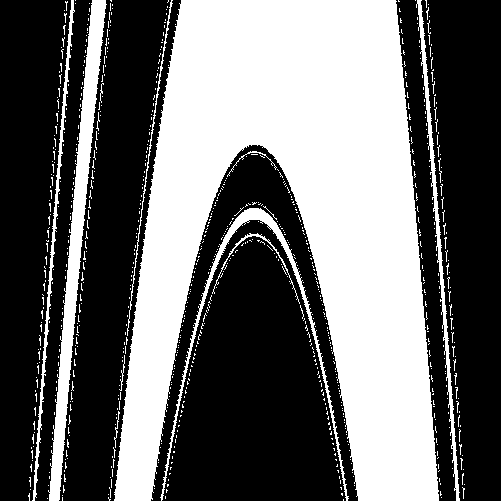
\includegraphics[width=\textwidth]{figure/section2/Henon-orbit-2--0*3.png}
\end{minipage}
\begin{minipage}[c][0.24\width]{0.24\textwidth}
   \centering
   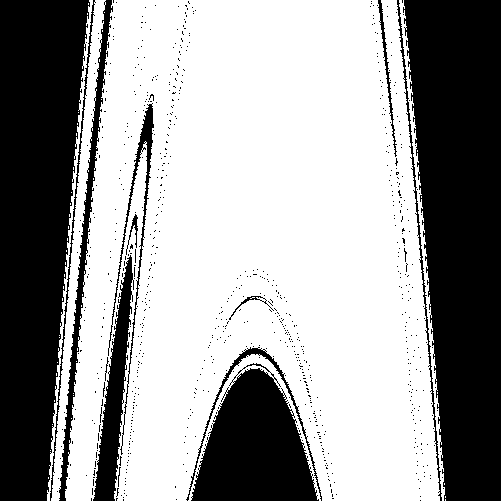
\includegraphics[width=\textwidth]{figure/section2/Henon-orbit-1*4--0*3.png}
\end{minipage}
\begin{minipage}[c][0.24\width]{0.24\textwidth}
   \centering
   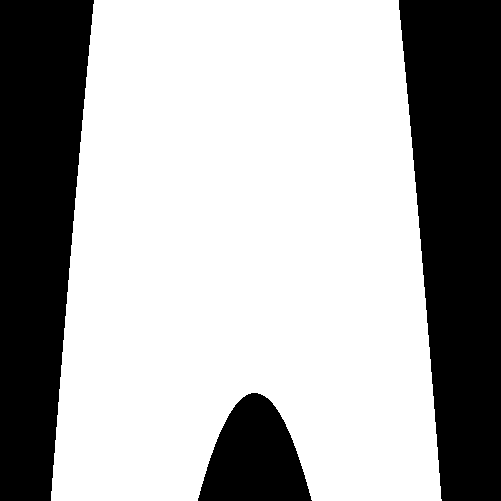
\includegraphics[width=\textwidth]{figure/section2/Henon-orbit-1*28--0*3.png}
\end{minipage}
\\[6ex]\caption{Initial condition square}\label{Initial-condition-square}
\end{figure}
(Parameter group $(a, b) = (0, 0.4), (2, -0.3), (1.4, -0.3), (1.28, -0.3))$







\subsection{Analysis of Henon map}
Now we focus on Henon map. Familiar with 1 dim map, it is necessary to define the sink and source as well as saddle.

\begin{definition}\textbf{Neighborhood}
\\\noindent Consider a $R^n$ space, called every point $x = (x_1, x_2, \ldots x_n)$ is a vector of $R^n$ space,
\\\noindent Define the \textbf{Euclidean Length} $|x| = \sqrt{x_1^2 + x_2^2 + \ldots + x_n^2}$, which is equal to norm;
\\\noindent And define the distance between two point $d(x, y) = |x - y|$;
\\\noindent Also, the \textbf{$\mathbf{\varepsilon}$-neighborhood} is 
$$
\forall \varepsilon > 0, \text{the }\varepsilon \text{-neighborhood of point }p, N_\varepsilon(p) \text{ is } \{x\in R^n | |x - p| < \varepsilon\} \text{, also define }N_\varepsilon^o(p) = N_\varepsilon(p)\backslash\{p\}
$$
\end{definition}

\begin{definition}\textbf{Sink and Source in High-dimension Map}
\\\noindent Let $f$ is a map on $R^n$, $p$ is a vector on $R^n$ which is the fixed point and $f(p) = p$ then 
\\\noindent If there is an $\varepsilon > 0$ s.t. $\forall x \in N_\varepsilon(p), \lim_{k \rightarrow \infty}f^k(x) = p$, then $p$ is a sink or attracting fixed point.
\\\noindent If $\forall x \in N_\varepsilon^o(p), \exists K \text{s.t.} \forall k > K, f^k(x) \notin N_\varepsilon(p)$, then called the point $p$ as source.
\end{definition}


We will explain these definitions with an example


\begin{example} \label{Henon-map-0-0*4}Analysis the sink point, source point and saddle of Henon map with parameter $a = 0, b = 0.4$
\end{example}

{\color{blue}
\begin{solution} Obviously, if we consider the funcion $f(x, y) = (-x^2 + 0.4y, x) = (x, y)$, then 
$$
 -0.2x^2 +0.4x = x \Rightarrow x_1 = 0, x_2 = -0.6
$$
So the fixed points are $(0, 0)$ and $(-0.6, -0.6)$. And now we have a new problem: how to confirm a fixed point is sink or source. Even the definition of sink and source are given above, we still need theory like Theo. \ref{sink-source-point}. But here, we can analysis the problem with simulator.$\blacksquare$\\[2ex]

\begin{figure}[H]
\begin{minipage}[c][0.25\width]{0.25\textwidth}
   \centering
   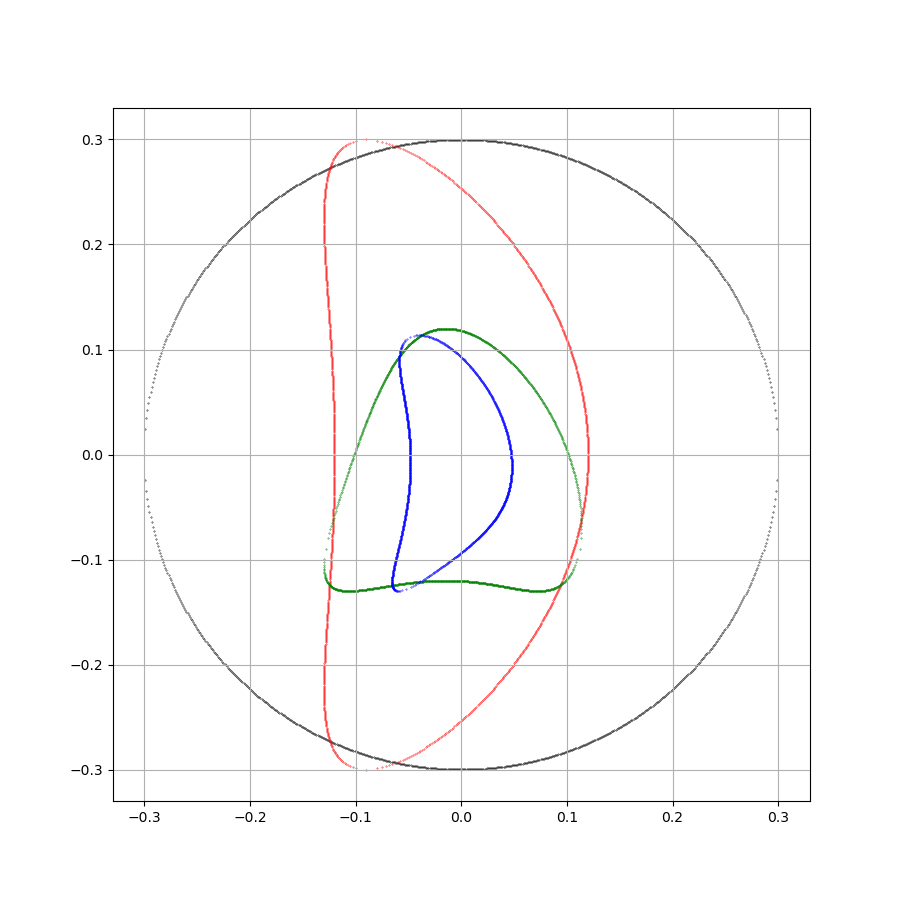
\includegraphics[width=\textwidth]{figure/section2/Henon-0-0*4-sink.png}
\end{minipage}
\begin{minipage}[c][0.45\width]{0.45\textwidth}
   \centering
   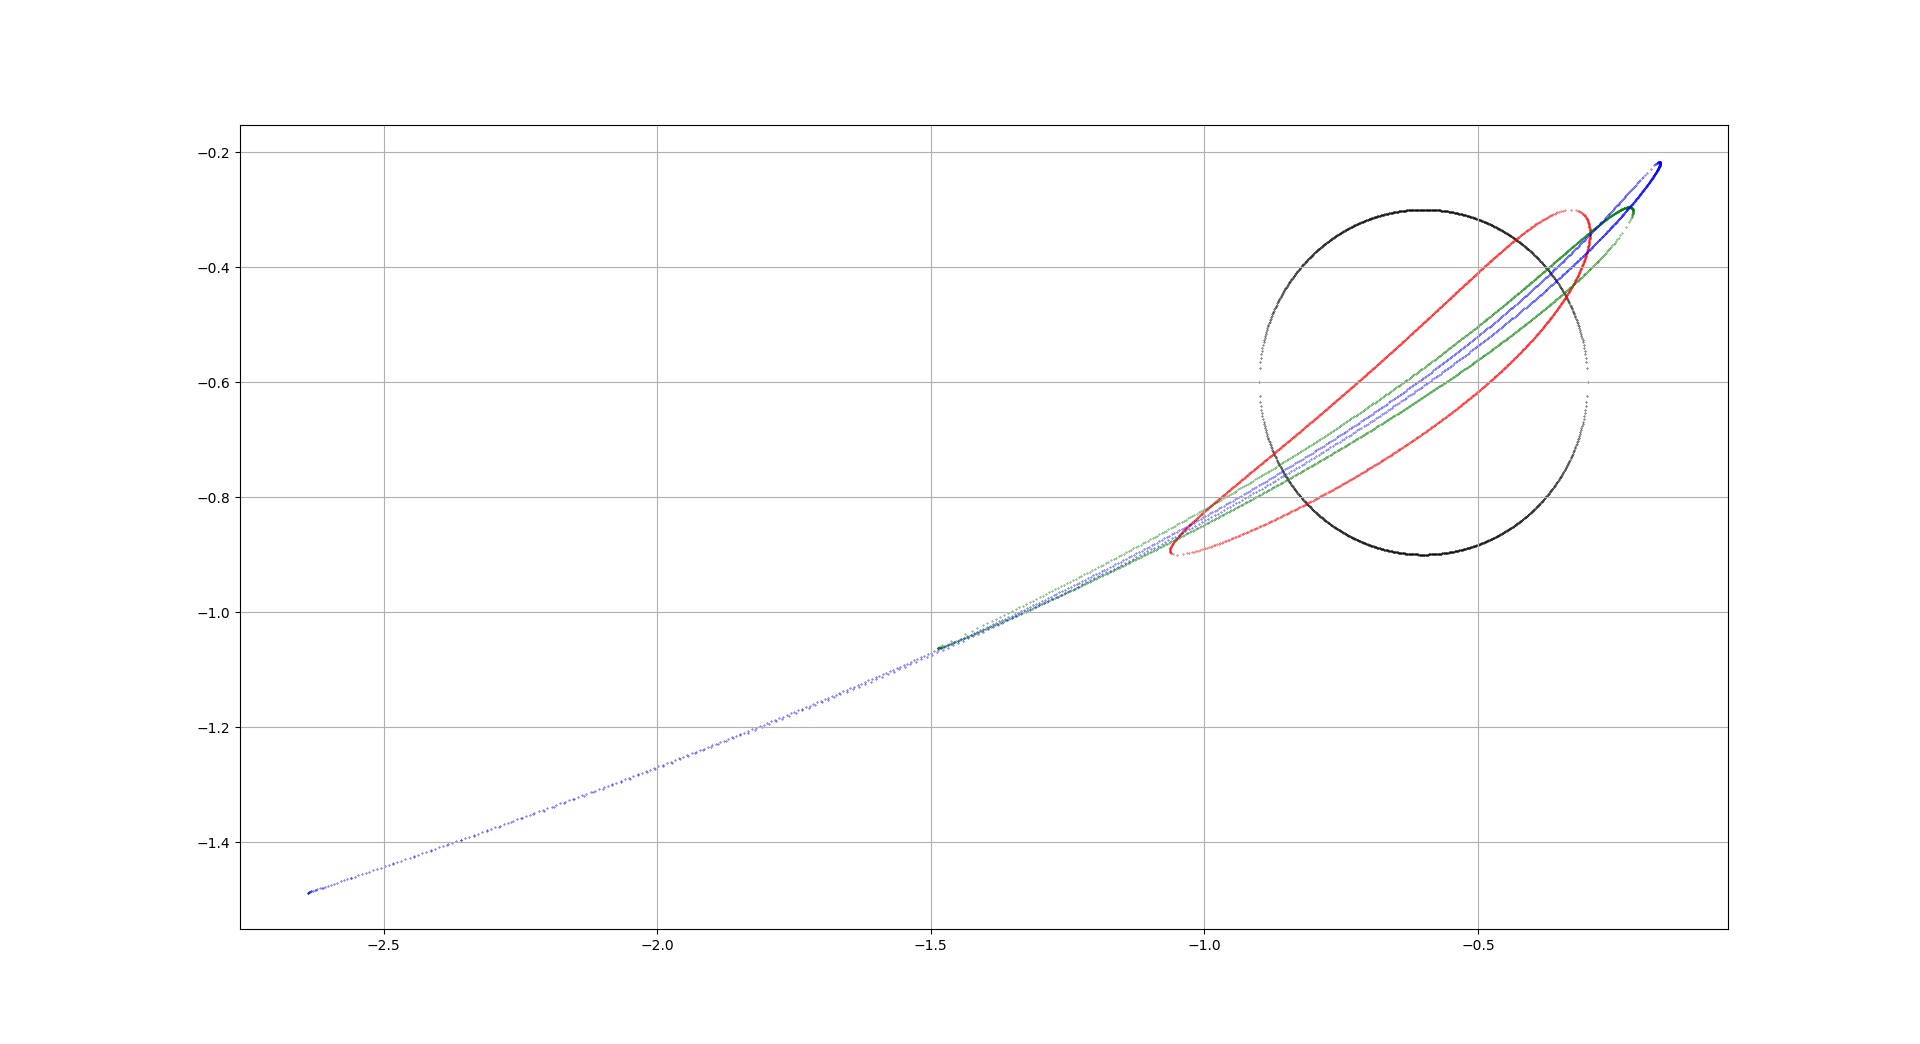
\includegraphics[width=\textwidth]{figure/section2/Henon-0-0*4-source.png}
\end{minipage}
\begin{minipage}[c][0.25\width]{0.25\textwidth}
   \centering
   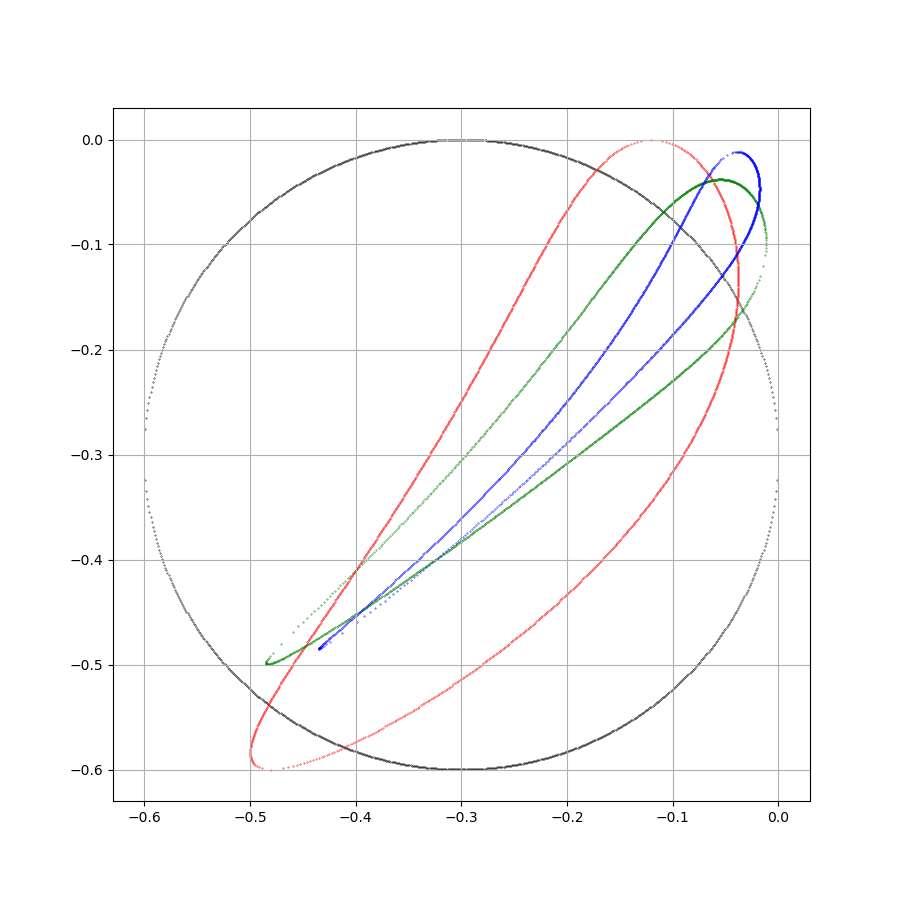
\includegraphics[width=\textwidth]{figure/section2/Henon-0-0*4-saddle.png} 
\end{minipage}
\\[3ex]\caption{Sink, source and saddle in Henon map with $a = 0, b = -0.4$}\label{sink-source-saddle-henon-map}
\end{figure}
(Order of color: {\color{black}Black(neighborhood)}, {\color{red} Red (Iter = 1)}, {\color{green} Green (Iter = 2)}, {\color{blue} Blue (Iter = 3)})

\end{solution}
}



To solve the problem we faced in e.g.\ref{Henon-map-0-0*4}, we will discuss the simple form of the high dimension maps.

\begin{definition}\textbf{High dimension linear map}
\\\noindent A map $A: R^m \rightarrow R^m$ is \textbf{linear} if $\forall a, b \in R, \forall x, y \in R^m$, $f(ax + by) = af(x) + bf(y)$. Equivalently, a lienar map $f(x)$ can be represented as multiplication by an $m \times m$ matrix.
\end{definition}

Now we consider a system s.t. $f(x) = Ax$, if $\lambda$ is eigenvalue and $\mathbf v$ is eigenvector of $A$, based on the definition fo eigenvalue and eigenvector, we have
Let $A$ have eigenvalue $\lambda$, based on the definition of eigenvalue, we have
$$
A\mathbf x = \lambda \mathbf v
$$
Then, for the initial point $\mathbf v$, we have
$$
A(\mathbf v) = A \mathbf v = \lambda \mathbf v
$$
let $\mathbf v_0 = \mathbf v, \mathbf v^n = A^n(\mathbf v)$, then
$$
\mathbf v_1 = A \mathbf v_0 = \lambda\mathbf v_0, \mathbf v_2 = A \mathbf v_1 = \lambda^2\mathbf v_1 \ldots \mathbf v_n = A \mathbf v_{n-1} = \lambda^{n}\mathbf v_0
$$
Futhermore, if we consider a system in random initial value $\mathbf x_0$, still define $\mathbf x_n = f(\mathbf x_{n-1})$, then 
$$
\mathbf x_n = f(\mathbf x_{n-1}) = A\mathbf x_{n-1} = Af(\mathbf x_{n-2}) = \ldots = A^n \mathbf x_0
$$





To analysis this problem, firstly we will review some theorems in algebra.







\begin{discussion}\textbf{Eigenvalue, eigenvector and Jordan normal form}
\\\noindent * We will consider a square matrix $A_{m\times m}$ s.t. $rank(A) = m$ in following discussion.\\[1ex]


  \noindent \textbf{[i] If $A$ have $m$ different Eigenvalue} 
\\\noindent Based on the discussion above, we know that it is the first step to analysis the $A^n$ to discribe all the linear system. Obviously, if A is a diagonal matrix, then the exponent of the matrix is easy and simple. 

\begin{theorem} Let $A$ is a diagonal matrix s.t. $A = diag(a_1, a_2, \ldots a_m)$, then $A^n = diag(a_1^n, a_2^n, \ldots a_m^n)$.
\end{theorem}

Furthermore, if matrix $A$ have $m$ different eigenvalue $\lambda_1, \lambda_2, \ldots, \lambda_m$ and $\mathbf v_i$ is the eigenvector of $\lambda_i$. Let
$$
\Lambda = diag(\lambda_1, \lambda_2, \ldots, \lambda_m), V = (\mathbf v_1, \mathbf v_2, \ldots \mathbf v_m)
$$
then we can easily prove that 
$$
A = V^{-1} \Lambda V
$$
And the calculation of $A^n$ is simple.
$$
A^n = V^{-1} \Lambda^n V = V^{-1} diag(\lambda_1^n, \lambda_2^n, \ldots, \lambda_m^n) V
$$

Now we back to consider the linear system, if $f(\mathbf x )= A \mathbf x$ and $A$ have $m$ different eigenvalue, then we know that 
$$
\mathbf x_{n} = A^n \mathbf x_0 = V^{-1} diag(\lambda_1^n, \lambda_2^n, \ldots, \lambda_m^n) V \mathbf x_0
$$

Based on the analysis in the section 1, we still want to analysis the convergence and divergence for ever system.
$$
\lim_{n \rightarrow \infty} x_{n} = V^{-1} diag(\lim_{n \rightarrow \infty}\lambda_1^n, \lim_{n \rightarrow \infty}\lambda_2^n, \ldots, \lim_{n \rightarrow \infty}\lambda_m^n) V \mathbf x_0
$$

Obviously, with the knowledge of sequence, if $|\lambda_i| \in [0, 1)$, then $\lim_{n \rightarrow \infty}\lambda_i^n = 0$ and the sequence is convergence. Also, if $|\lambda_i| \in (1, +\infty)$, then $\lim_{n \rightarrow \infty}\lambda_i^n = \infty$ and the sequence is divergence. So we have this conclusion.


\begin{theorem}\label{sink-source-saddle-linear-system}\textbf{Sink, source and saddle in linear system}
\\\noindent Consider a linear system $f(\mathbf x) = A \mathbf x$, where $A$ is a square matrix in $m$ dimension. If the eigenvalue of $A$ are $\lambda_1, \lambda_2, \ldots \lambda_m$ and
\\\noindent \textbf{[i]} $\forall i \in 1, 2, \ldots, m, |\lambda_i| < 1$, then the origin point is sink.
\\\noindent \textbf{[ii]} $\forall i \in 1, 2, \ldots, m, |\lambda_i| > 1$, then the origin point is source.
\\\noindent \textbf{[iii]} $\{i | |\lambda_i| < 1\} \neq \varnothing \land \{j | |\lambda_j| > 1\} \neq \varnothing$, that means, if at least one eigenvalue are absolute smaller than one and at least one is upper than one, then the origin point is saddle.\\
\end{theorem}





  \noindent \textbf{[ii] If $A$ have at least two equal eigenvalue} 
\\\noindent We can transfrom the matrix $A$ with Jordan normal form rather than eigenvalue diagonal matrix.
\\\noindent Consider the matrix $A_{m\times m}$ and the eigenvalue $\lambda_{1}, \lambda_{2}, \ldots, \lambda_{k}$ are $r_1, r_2, \ldots r_k$ multiple root of function $|\lambda I - A| = 0$, which satisfied the definition of eigenvalue, and $k < m$, $\sum_{i = 1}^{k} r_i = m$, $I = diag(1, 1, 1, \ldots, 1)$. 
\\\noindent Then for every $r_i$ multiple eigenvalue $\lambda_i$, $\exists \mathbf v_{i1}, \mathbf v_{i2}, \ldots \mathbf v_{i r_i}$ s.t.
$$
|\lambda I - A|\mathbf v_{i1} = 0, |\lambda I - A|\mathbf v_{ij+1} = \mathbf v_{ij}(j = 1, 2, \ldots r_i - 1)
$$
We can still structure the $V$ matrix same as $V$ in \textbf{[i]}, and we can also represent the diagonal eigenvalue matrix $\Lambda$ to the \textbf{ Jordan normal form matrix} $J$ which satisfied 
$$
J = \left[
\begin{array}{cccc}
J_{1} \\
& J_{2} \\
& & \ldots \\
& & & J_{k}
\end{array}
\right] = diag(J_1, J_2, \ldots J_k) \text{, where } J_i =\left[
\begin{array}{ccccc}
\lambda_i & 1 \\
& \lambda_i & 1 \\
& & \ldots & \ldots \\
& & & \lambda_i & 1 \\
& & & & \lambda_i
\end{array} \right]
$$
is $r_i$ dimension square matrix called \textbf{Jordan block}

Based on the calculation of block matrix we found that
$$
A^n = V^{-1} J^n V = V^{-1} diag(J_1^n, J_2^n, \ldots, J_k^n) V
$$

So familiar with the discussion in \textbf{[i]}, now it is necessary to discuss the $J_i^n$. On the other hand, we know that for ever Jordan block, we have
$$
J_i^n = \left[
\begin{array}{ccccc}
\lambda_i^n & (^n_1)\lambda_i^{n-1} & (^n_2)\lambda_i^{n-2} & \ldots      & (^n_{r_i})\lambda_i^{n-r_i}        \\
            & \lambda_i^n           & (^n_1)\lambda_i^{n-1} & \ldots      & (^n_{r_{i-1}})\lambda_i^{n-r_i+1}  \\
            &                       & \ldots                & \ldots      & \ldots                             \\
            &                       &                       & \lambda_i^n & (^n_1)\lambda_i^{n-1}              \\
            &                       &                       &             & \lambda_i^n
\end{array} \right]
$$ 

Obviously, for ever element on the diagonal, the Theo. \ref{sink-source-saddle-linear-system} still established. To proved that, we will prove the following theorem firstly.

\begin{theorem} \label{exp_Jordan}Let $J_i$ is a Jordan block with eigenvalue $\lambda_i$. 
\\\noindent \textbf{[i]} If $|\lambda_i| < 1$, then $\lim_{n \rightarrow \infty} J_i^n = 0$
\\\noindent \textbf{[ii]} If $|\lambda_i| > 1$, then $\lim_{n \rightarrow \infty} J_i^n = \infty$
\end{theorem}
{\color{blue}
\begin{proof} Consider a element $(^n_k)\lambda_i^{n-k}$ of $J_i$, then 
$$
\lim_{n \rightarrow \infty}(^n_k)\lambda_i^{n-k} = \lim_{n \rightarrow \infty}\left({n(n-1)\ldots(n-k) \over 1\cdot 2 \cdot \ldots \cdot k} \lambda_i^{n-k}\right)
$$

As the ${n(n-1)\ldots(n-k) \over 1\cdot 2 \cdot \ldots \cdot k}$ is a polynomial of $n$ in $k$ dimension, so $\exists a_1, a_2, \ldots a_k \in R$ s.t. 
$$
\lim_{n \rightarrow \infty}(^n_k)\lambda_i^{n-k} = \lim_{n \rightarrow \infty}\left(\sum_{p = 1}^{k} a_p n^p\right)\lambda_{n - k} = \sum_{p = 1}^{k} \lim_{n \rightarrow \infty}(a_p n^p \lambda_i^{n-k})
$$
Finally, we found, if $|\lambda_i| > 1$, then $\lim_{n \rightarrow \infty}(^n_k)\lambda_i^{n-k} = \infty$ and if $|\lambda_i| < 1$, then $\lim_{n \rightarrow \infty}(^n_k)\lambda_i^{n-k} = 0$ and the Theo. \ref{exp_Jordan} is established. $\blacksquare$
\end{proof}
}

\end{discussion}


As for the non-linear problem, a wildly used method is \textbf{Jacobian matrix}


\begin{definition}\textbf{Jacobian matrix}
\\\noindent Let $\mathbf f = (f_1, f_2, \ldots f_m)$ be a map on $R^m$ and $\mathbf p \in R^m$ is a point on $R^m$ space. The \textbf{Jacobian matrix} of $\mathbf f$ at $\mathbf p$ is the matrix 
$$
D\mathbf f(\mathbf p) = \left[
\begin{array}{cccc}
{\partial f_1 \over \partial x_1}(\mathbf p) & {\partial f_1 \over \partial x_2}(\mathbf p) & \ldots {\partial f_1 \over \partial x_m}(\mathbf p) \\
{\partial f_2 \over \partial x_1}(\mathbf p) & {\partial f_2 \over \partial x_2}(\mathbf p) & \ldots {\partial f_2 \over \partial x_m}(\mathbf p) \\
\ldots & \ldots & \ldots & \ldots \\
{\partial f_m \over \partial x_1}(\mathbf p) & {\partial f_m \over \partial x_2}(\mathbf p) & \ldots {\partial f_m \over \partial x_m}(\mathbf p) \\
\end{array} \right]
$$
\end{definition}

Jacobian matrix is a linearization estimation of a non-linear system that we can assume the derivative of the system near the point $\mathbf p$ is $D\mathbf f(\mathbf p)$. That means, instead of origin non-linear system, we can analysis the estimated system $\mathbf f_1(\mathbf x) = D\mathbf f(\mathbf p) \mathbf x$ where $x \in N(\mathbf p, \varepsilon)$ and $\varepsilon$ is a certain constant. Based on the Theo. \ref{sink-source-saddle-linear-system}, it is easy to improve the following conclusion.

\begin{theorem}\label{sink-source-saddle-Jacobian-matrix}\textbf{Sink, source and saddle in non-linear system}
\\\noindent Consider a non-linear system $\mathbf f(\mathbf x)$ and a fixed point $\mathbf p \in R^m$ s.t. $\mathbf f (\mathbf p) = \mathbf p$. If the Jacobian matrix of $\mathbf f$ at $\mathbf p$ is $D\mathbf f(\mathbf p)$, and $\Lambda$ are eigenvalue set of matrix $D\mathbf f(\mathbf p)$
\\\noindent \textbf{[i]} $\forall \lambda_i \in \Lambda  |\lambda_i| < 1$, then the $\mathbf p$ is a sink point.
\\\noindent \textbf{[ii]} $\forall \lambda_i \in \Lambda  |\lambda_i| > 1$, then the $\mathbf p$ is a source point.
\\\noindent \textbf{[iii]} $\{\lambda_i \in \Lambda | |\lambda_i| < 1\} \neq \varnothing \land \{\lambda_i \in \Lambda | |\lambda_i| > 1\} \neq \varnothing$, that means, if at least one eigenvalue are absolute smaller than one and at least one is upper than one, then the $\mathbf p$ is a saddle point.
\end{theorem}


Finally, we can analysis the property of fixed point in e.g. \ref{Henon-map-0-0*4}.
{\color{blue}
\begin{solution} We can consider the Henon map directly
$$
f(x, y) = (a - x^2 + by, x)  \Rightarrow Df(x, y) = \left[
\begin{array}{cc}
-2x & b \\
1 & 0 
\end{array} \right] 
$$
Let $\lambda$ are eigenvalue, then
$$
|\lambda I - Df(x, y)| = 0 \Rightarrow \left|
\begin{array}{cc}
-2x- \lambda & b \\
1 & -\lambda
\end{array} \right| = 0 \Rightarrow \lambda^2 + 2x\lambda - b = 0 \Rightarrow \lambda_{12} = {-x \pm\sqrt{x^2 + b}}
$$
When $(a, b) = (0, 0.4)$
$$
\text{If } (x, y) = (0, 0) \text{, then }|\lambda_{12}| = |-x\pm\sqrt{x^2 + b}| = |\sqrt{0.4}| < 1
$$
$$
\text{If } (x, y) = (0.6, 0.6) \text{, then }|\lambda_{12}| = |-x\pm\sqrt{x^2 + b}| = |-0.6 \pm \sqrt{0.76}| \Rightarrow |\lambda_1| = 1.472 > 1, |\lambda_2| = 0.272 < 1
$$
Finally, we proved that $(0, 0)$ is sink and $(-0.6, -0.6)$ is saddle just as what we found on simulation.$\blacksquare$


\end{solution}
}








\subsection{Stability and matrix periodic}
We found this conclusion based on the discussion above.

\begin{conclusion} The value of Jacobian matrix of a Henon map is just relevant to variable $x$ and parameter $b$. That means, if we reduce the dimension of parameter and fixed $b$ as $b_0$, then the property of fixed point will be determined only with variable $x$.
\end{conclusion}

As $y_{n+1} = x_n$, so we can just analysis the bifurcation of $a - x_{\infty}$ with random initial point.


If we consider the fixed point of system with arbitrary paremeter grou $(a, b)$, we found that the fixed point will satisfied 
\begin{flalign}
& x^2 + (1 - b)x - a = 0 \Rightarrow x = {1\over 2} (b-1) \pm\sqrt{(b-1)^2 + 4 a} & \label{formula-21}
\end{flalign}

and the fixed point is $(x, y) = ({1\over 2} (b-1) \pm\sqrt{(b-1)^2 + 4 a}, {1\over 2} (b-1) \pm\sqrt{(b-1)^2 + 4 a})$, so we have the Jacobian matrix at this fixed point as 
$$
Df(x, y) = \left[
\begin{array}{cc}
(b-1) \pm\sqrt{(b-1)^2 + 4 a} & b \\
1 & 0 
\end{array} \right] \text{, and the eigenvalue $\lambda_i$ satisfied }
$$
\begin{flalign}
& \lambda^2 - [(b-1) \pm\sqrt{(b-1)^2 + 4 a}]\lambda - b = 0 & \label{formula-22}
\end{flalign}

Then we can found the property of sink and source in every fixed point easily.

Now we focus on periodic-k orbit. Firstly, we still plot the bifurcation diagram of Henon map.

\begin{figure}[H]
\begin{center}
\includegraphics[width=0.6\textwidth]{figure/section2/Henon-orbit-bf-a--0*4.png}
\caption{Bifurcation diagram for Henon map ($b = 0.4$)}\label{Henon-map-b=0*4-BF}
\end{center}
\end{figure}



That is simple to analysis the influence of parameter. In following plots, $b \equiv 0.4$ and $a = 0.9, 0.988, 1.0, 1.0293, 1.045, 1.2$. We found $a = 0.9$ is a periodic-4 sink, $a = 0.988$ is a periodic-16 sink, $a = 1.0$ is a four-piece attractor, $a = 1.0293$ is a periodic-10 sink, $a = 1.045$ is two-piece attractor and the points of an orbit alternate between the pieces. Finally $a = 1.2$ two pieces have merged to form one-piece attractor.

\begin{definition}\textbf{Attractor} An attractor is a set of numerical values toward which a system tends to evolve, for a wide variety of starting conditions of the system.
\\\noindent Futuermore, in discrete time, we called the orbit of a system as periodic-k orbit. However in chaotic orbit, the solution set is a continuous (or uncountable) set. And we called this orbit as attractor.
\end{definition}

We will discuss the relationship between matrix and periodic-k orbit. But before that, it is necessary to introduce some new definition.

\begin{definition} A map $\mathbf f$ on $R^m$ is \textbf{one-to-one} if and only if $\mathbf f(\mathbf v_1) \mathbf f(\mathbf v_2) \Leftrightarrow \mathbf v_1 = \mathbf v_2$
\end{definition}





\begin{figure}[H]
\begin{minipage}[c][0.32\width]{0.32\textwidth}
   \centering
   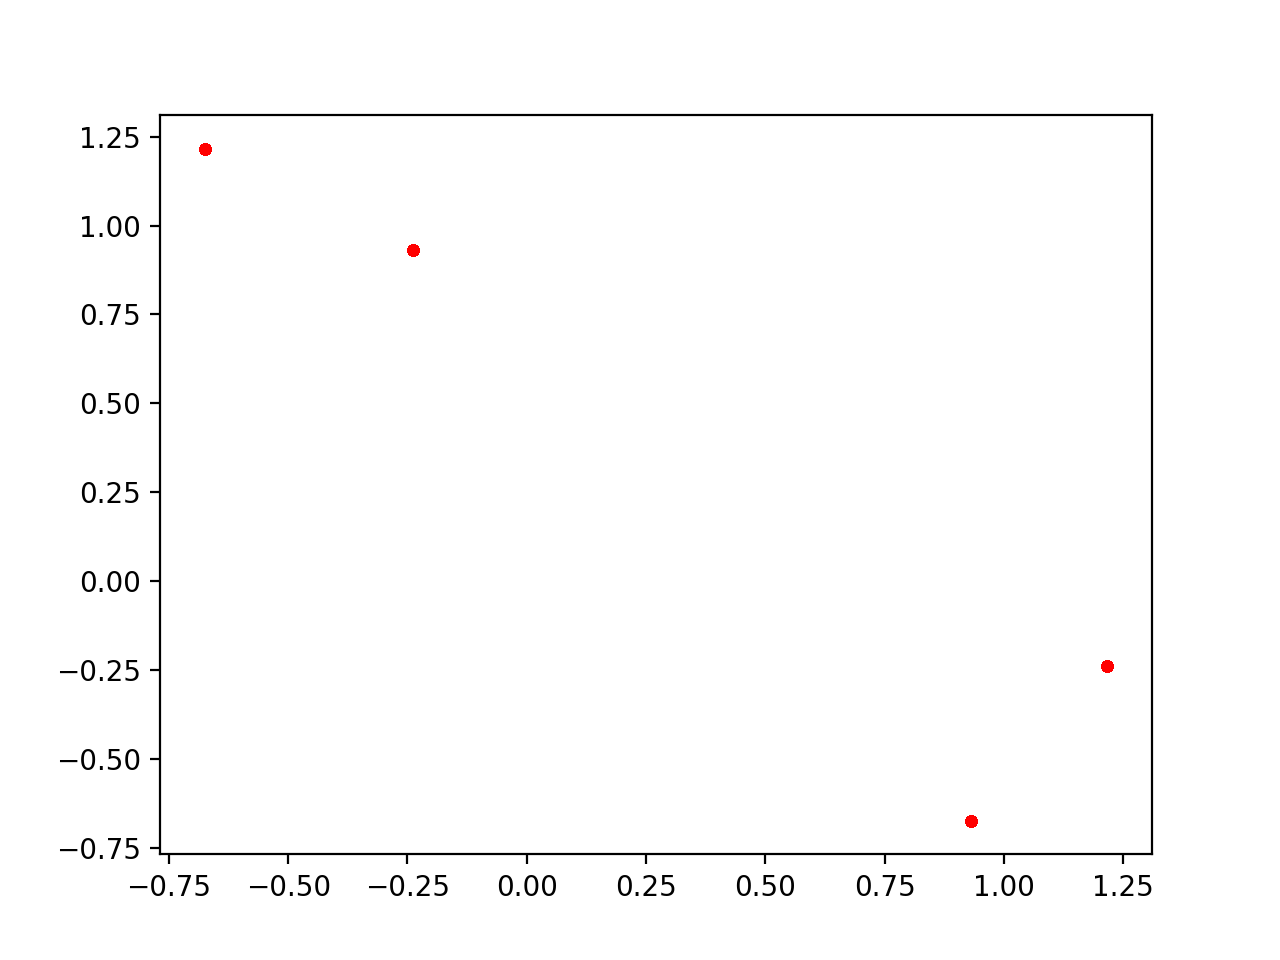
\includegraphics[width=\textwidth]{figure/section2/Henon-attractor-0*9-0*4.png}
\end{minipage}
\begin{minipage}[c][0.32\width]{0.32\textwidth}
   \centering
   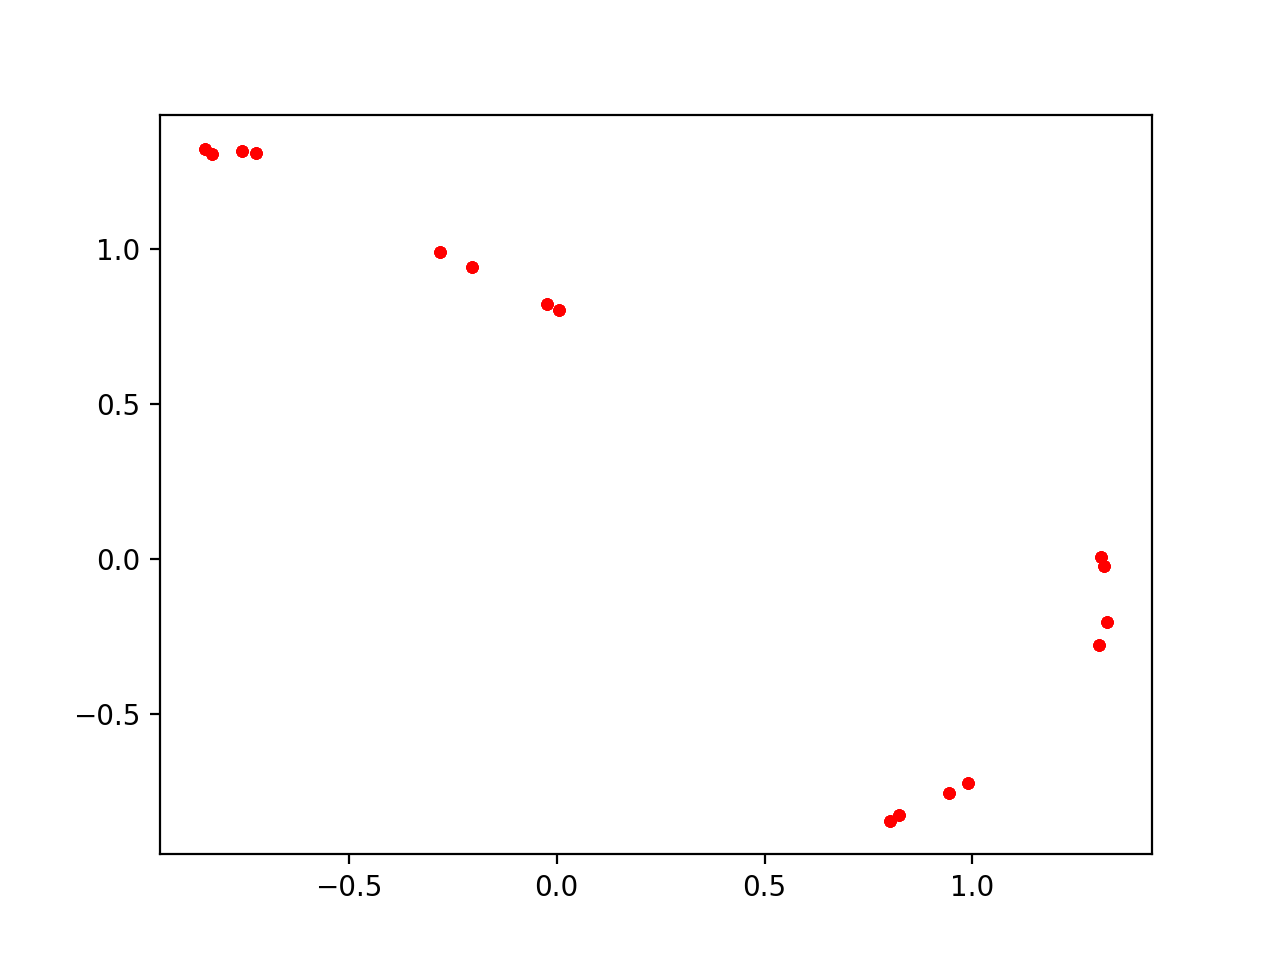
\includegraphics[width=\textwidth]{figure/section2/Henon-attractor-0*988-0*4.png}
\end{minipage}
\begin{minipage}[c][0.32\width]{0.32\textwidth}
   \centering
   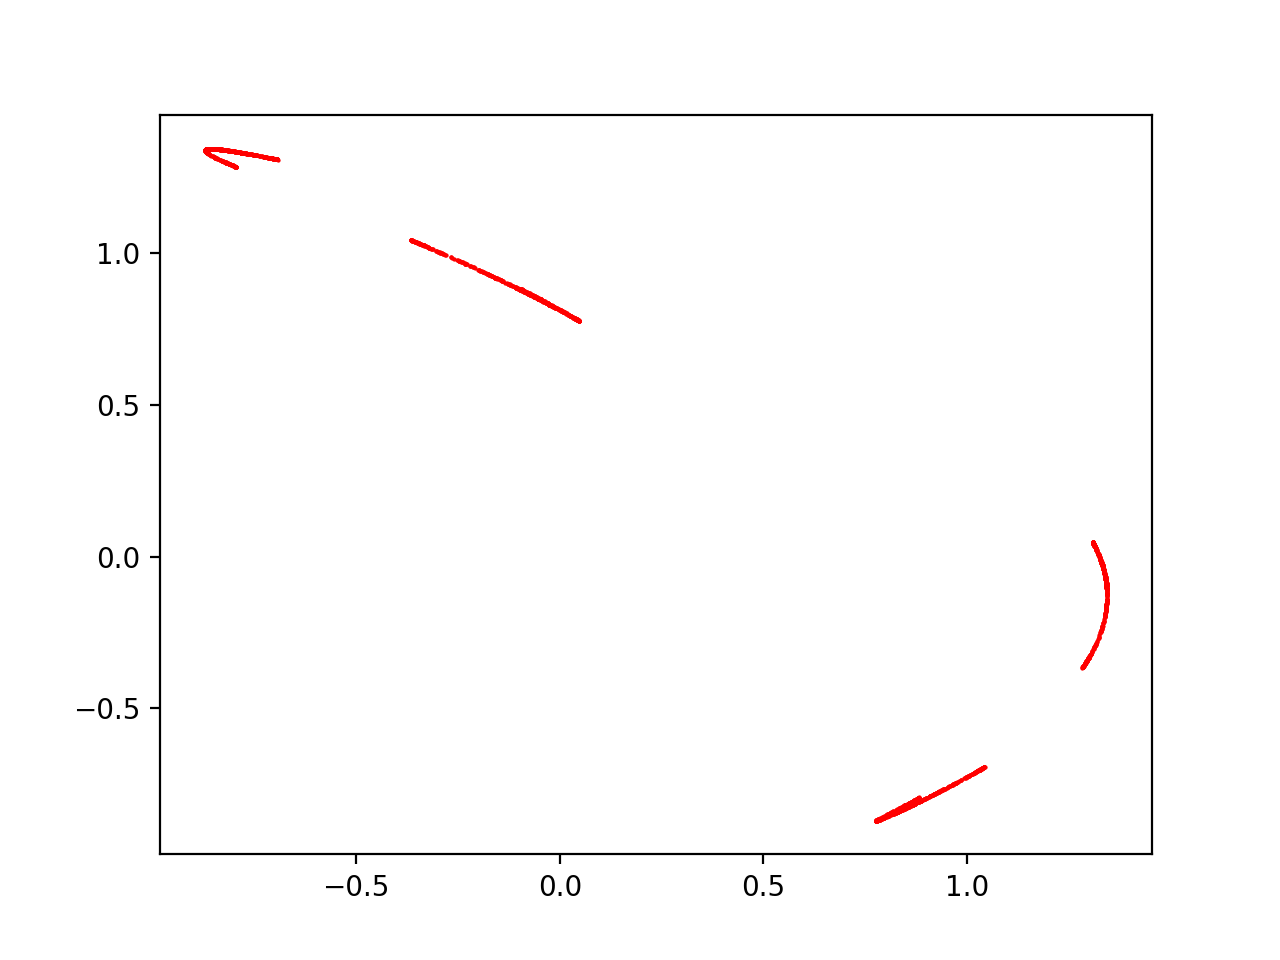
\includegraphics[width=\textwidth]{figure/section2/Henon-attractor-1*0-0*4.png}
\end{minipage}
\\[12ex]
\begin{minipage}[c][0.32\width]{0.32\textwidth}
   \centering
   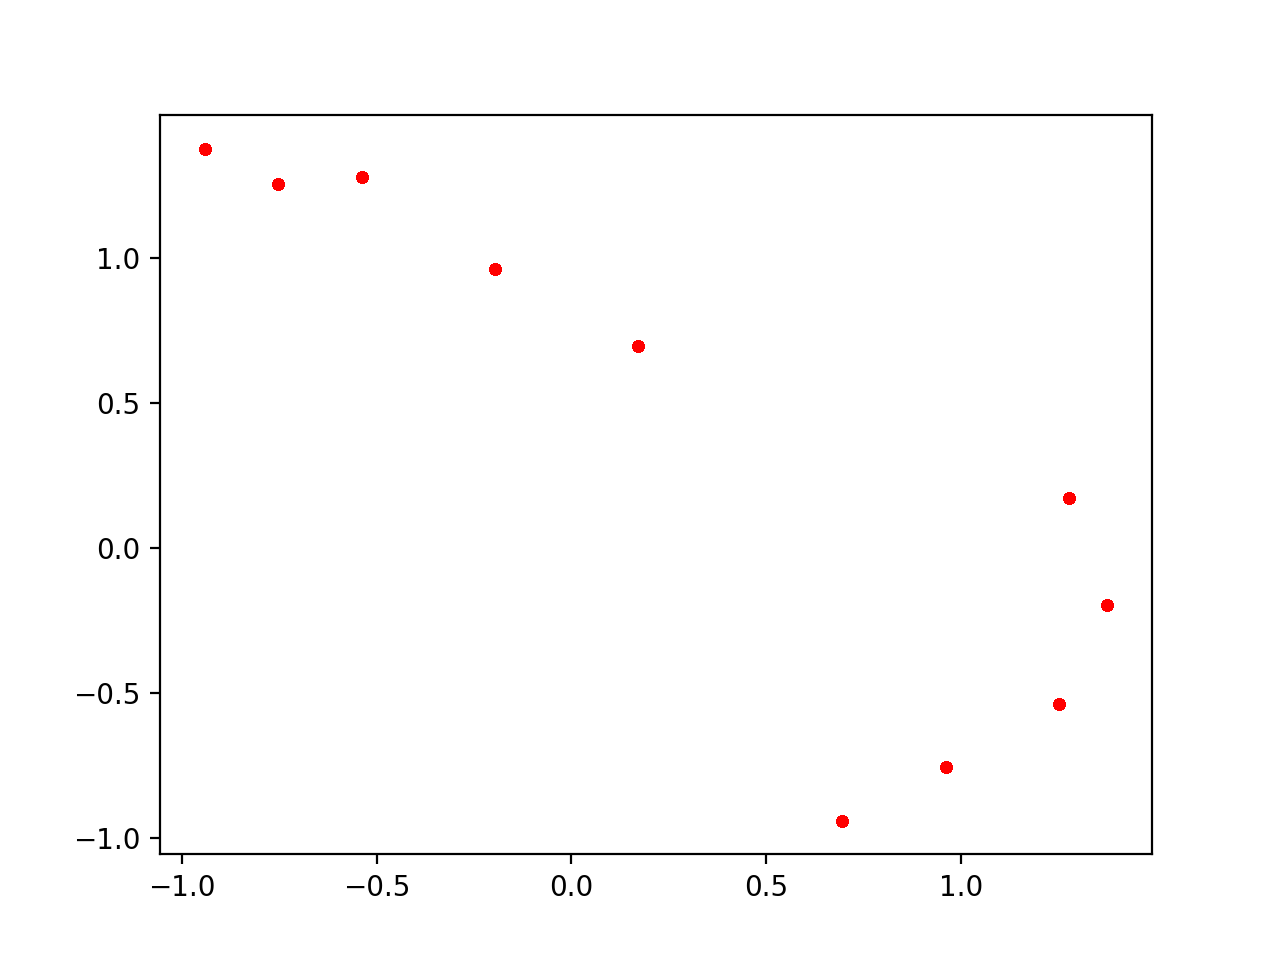
\includegraphics[width=\textwidth]{figure/section2/Henon-attractor-1*0293-0*4.png}
\end{minipage}
\begin{minipage}[c][0.32\width]{0.32\textwidth}
   \centering
   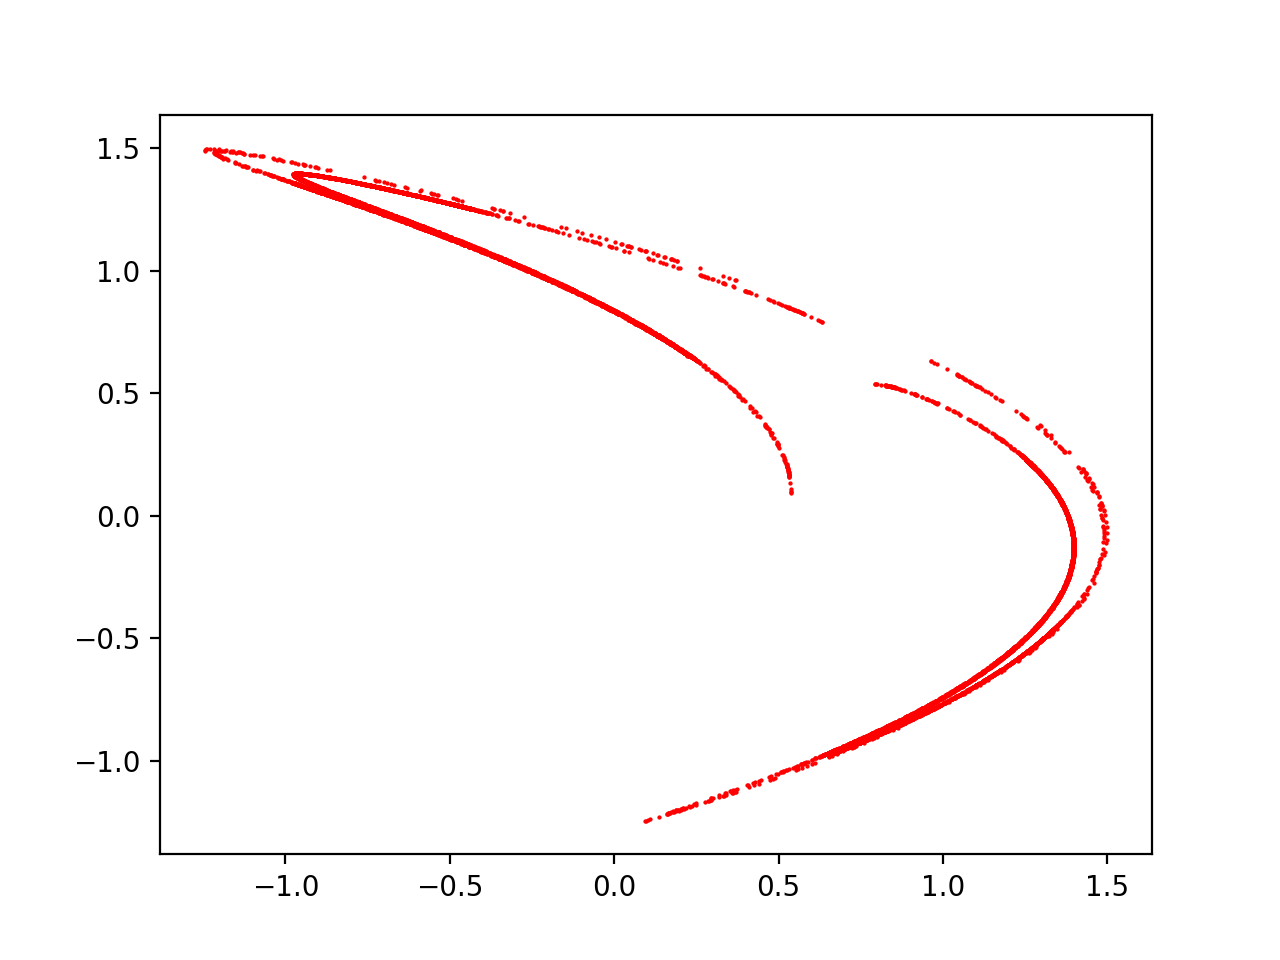
\includegraphics[width=\textwidth]{figure/section2/Henon-attractor-1*045-0*4.png}
\end{minipage}
\begin{minipage}[c][0.32\width]{0.32\textwidth}
   \centering
   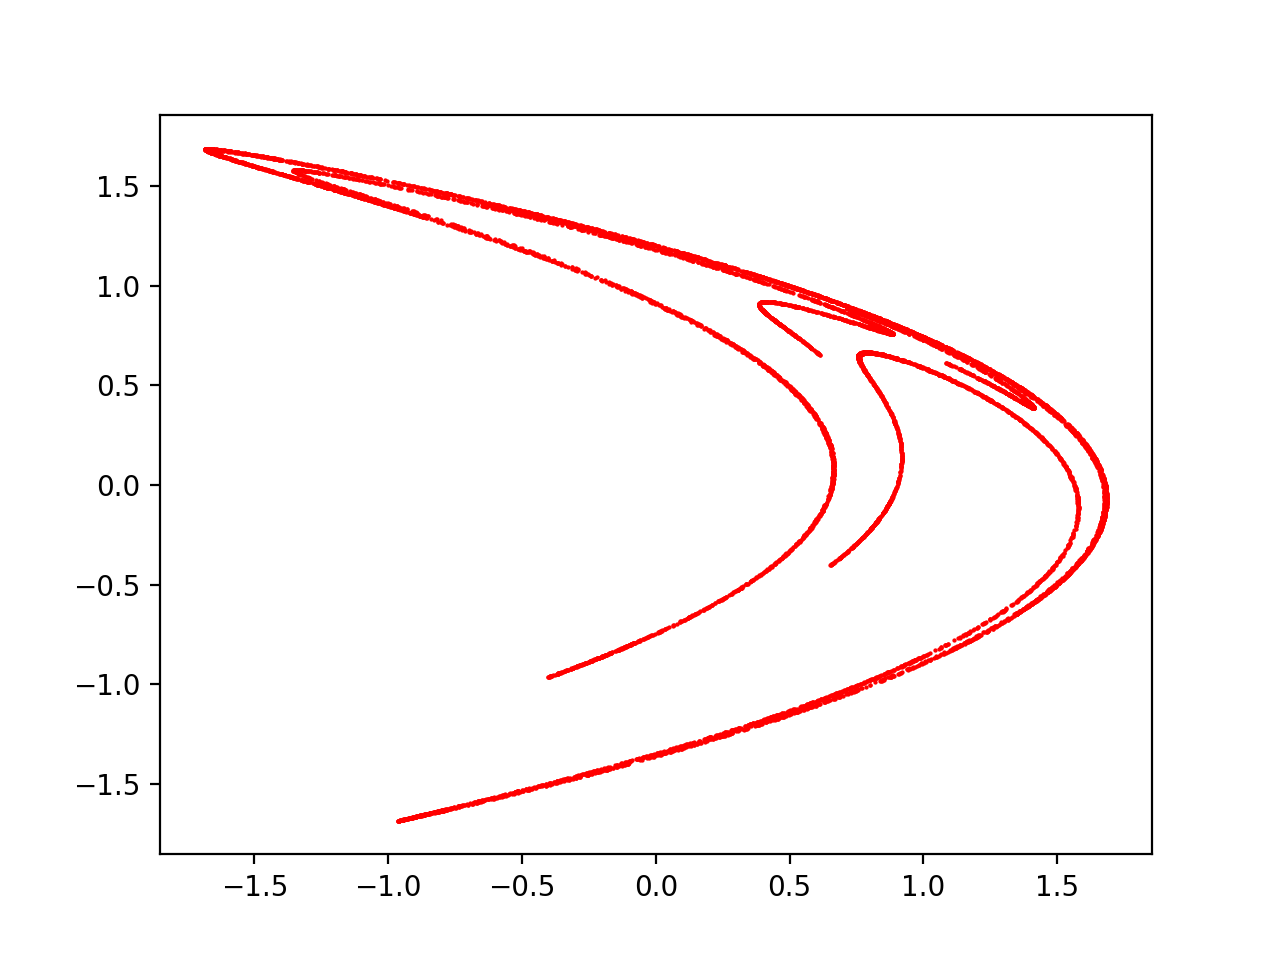
\includegraphics[width=\textwidth]{figure/section2/Henon-attractor-1*2-0*4.png}
\end{minipage}
\\[4ex]\caption{Attractor of Henon map in different parameter}\label{attractor-Henon-map}
\end{figure}


\begin{definition}\textbf{Inverse map}
\\\noindent Consider a one-to-one map $\mathbf f$ on $R^m$. The inverse map $\mathbf f^{-1}$ is automatically exists and satisfied $\forall \mathbf v \in D \subset R^m, \mathbf f(\mathbf f^{-1})(\mathbf v) = \mathbf f^{-1}(\mathbf f)(\mathbf v) = \mathbf v$, where $D$ is domain of map.
\end{definition}

For instance, a one-to-one map $f(x) = 2x$ have an inverse map $f^{-1} = {x/2}$. Obviously, for every linear map $\mathbf f(\mathbf x) = A \mathbf x, \exists f^{-1}(\mathbf x) = A^{-1} \mathbf x$.

\begin{theorem} For every $R^m$ linear map $\mathbf f(\mathbf x) = A \mathbf x$ and $A$ s.t. $rank(A) = m$, the inverse map $f^{-1}$ always be existed.
\end{theorem}
{\color{blue}
\begin{proof}\textbf{[i]} If $A$ have $m$ different eigenvalue, then $A = V\Lambda V$ where $\Lambda = diag(\lambda_1, \lambda_2, \ldots, \lambda_m), V = (\mathbf v_1, \mathbf v_2, \ldots ,\mathbf v_m)$ where $\lambda_i$ is eigenvalue and $\mathbf v_1$ is eigenvector. Then 
$$
A^{-1} = \left(V^{-1} \Lambda V\right)^{-1} = V \Lambda^{-1} V^{-1} = V diag\left({1 \over \lambda_1}, {1 \over \lambda_2}, \ldots, {1 \over \lambda_m}\right) V^{-1}
$$
\\\noindent \textbf{[ii]} If $A$ have $p < m$ different eigenvalue, based on the Jordan normal form, we still have $J, V$ s.t. $A = V^{-1} J V$ and $J = diag(J_1, J_2, \ldots J_k)$ where $J_i$ is Jordan block based on the eigenvalue $\lambda_i$. And now the problem is prove that for evert Jordan block, the inverse block always be existed.
\\\noindent Obviously, $J_i = \lambda_i I + N$ where
$$
N = \left[
\begin{array}{ccccc}
0 & 1 & 0 & \ldots & 0 \\
0 & 0 & 1 & \ldots & 0 \\
\ldots & \ldots & \ldots & \ldots & \ldots \\
0 & 0 & 0 & \ldots & 1 \\
0 & 0 & 0 & \ldots & 0 \\
\end{array} \right]
$$

And it is simple to found that $N^m = \mathbf 0_{m\times m}$. Based on the Taylor expansion, we have 
$$
J_i^{-1} = \lambda_i^{-1} (I + \lambda_i^{-1} N + \lambda_i^{-2} N^2 - \ldots + (-\lambda_i)^{-n+1}N^{n-1})
$$

Although the inverse of Jordan block is not a Jordan block of $1/\lambda_i$, it is still exists and we proved the theorem. $\blacksquare$
\end{proof}
}







%~~~~~~~~~~~~~~~~~~~~~~~~~~~~~~~~~~~~~~~~~~~~~~~~~~~~~~~~~~~~~~~~~~~~~~~~~~~~~~~~~~~~~~~~~~~~~~~~~~~~~















%~~~~~~~~~~~~~~~~~~~~~~~~~~~~~~~~~~~~~~~~~~~~~~~~~~~~~~~~~~~~~~~~~~~~~~~~~~~~~~~~~~~~~~~~~~~~~~~~~~~~~
\newpage
\section{Chaos}

We discussed the Henon map in last section. However, different from the section 1, Logistic map has been wildly used in application problems, we talked less about why we are interested in this model. So, in this section, we will mainly introduce the motivation.




\subsection{Lorenz system, Henon map and Poincare section}



\begin{discussion} \textbf{Why are we intersted in Henon map?}
\\\noindent First of all, it is necessary to introduce a continuous model. The Lorenz system is a system of ordinary differential equations which notable for having chaotic solutions for certain parameter values and initial conditions. In particular, the Lorenz attractor is a set of chaotic solutions of the Lorenz system.

\begin{problem}\textbf{Lorenz model}
\\\noindent Lorenz model is a system of three ordinary differential equations now known as the Lorenz equations:
$$
{dx \over dt} = \sigma(y - x)
$$
$$
{dy \over dt} = x(\rho - z) - y
$$
$$
{dz \over dt} = xy - \beta z
$$
where $\sigma, \rho, \beta$ are parameters.
\end{problem}

It is continuous problem, however, based on the knowledge in numerical analysis, we can discrete the continuous to discrete problem in several ways.\footnote{EDWARD N LORENZ’S 1963 PAPER, “DETERMINISTIC NONPERIODIC FLOW”, IN JOURNAL OF THE ATMOSPHERIC SCIENCES, VOL 20, PAGES 130–141} 

We can reconstruct the Lorenz equation, or a normal continuous dynamical system as 
$$
{dX_i\over dt} = F_i(X_1, X_2, \ldots X_m), i = 1, 2, \ldots m
$$
which is a m-dim dynamical system and $t$ is single independence variable. To simplify this problem, we choose a initial time $t_0$ and time increment $\Delta t$, then let 
$$
X_{i, n} = X_i (t_0 + n \Delta t)
$$
we have several ways to aproximate the equations.



{\color{blue}
\begin{solution}\textbf{[i] Auxiliary approximations} $X_{i, n+1} = X_{i, n} + F_i(P_n)\Delta t$
\\\noindent \textbf{[ii] Centered difference procedure} $X_{i, n+1} = X_{i, n-1} + 2F_i(P_n)\Delta t$
\\\noindent \textbf{[iii] Double-approximation procedure} $X_{i, n+1} = X_{i, n} + {1\over 2}(F_i(P_n) + F_i(P_{n+1}))\Delta t$
\end{solution}
}


Even solve this group of function directly is difficult, it is not difficult to find the numerical solution. \\[2ex]

\begin{figure}[H]
\begin{minipage}[c][0.29\width]{0.29\textwidth}
   \centering
   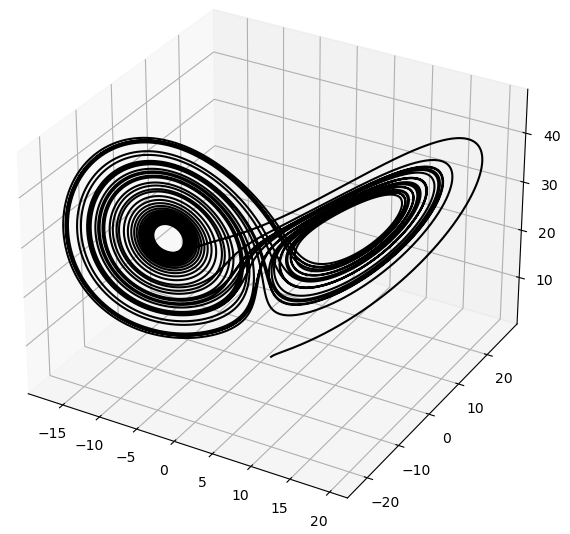
\includegraphics[width=\textwidth]{figure/section2/Lorenz.png}
\end{minipage}
\begin{minipage}[c][0.4\width]{0.4\textwidth}
   \centering
   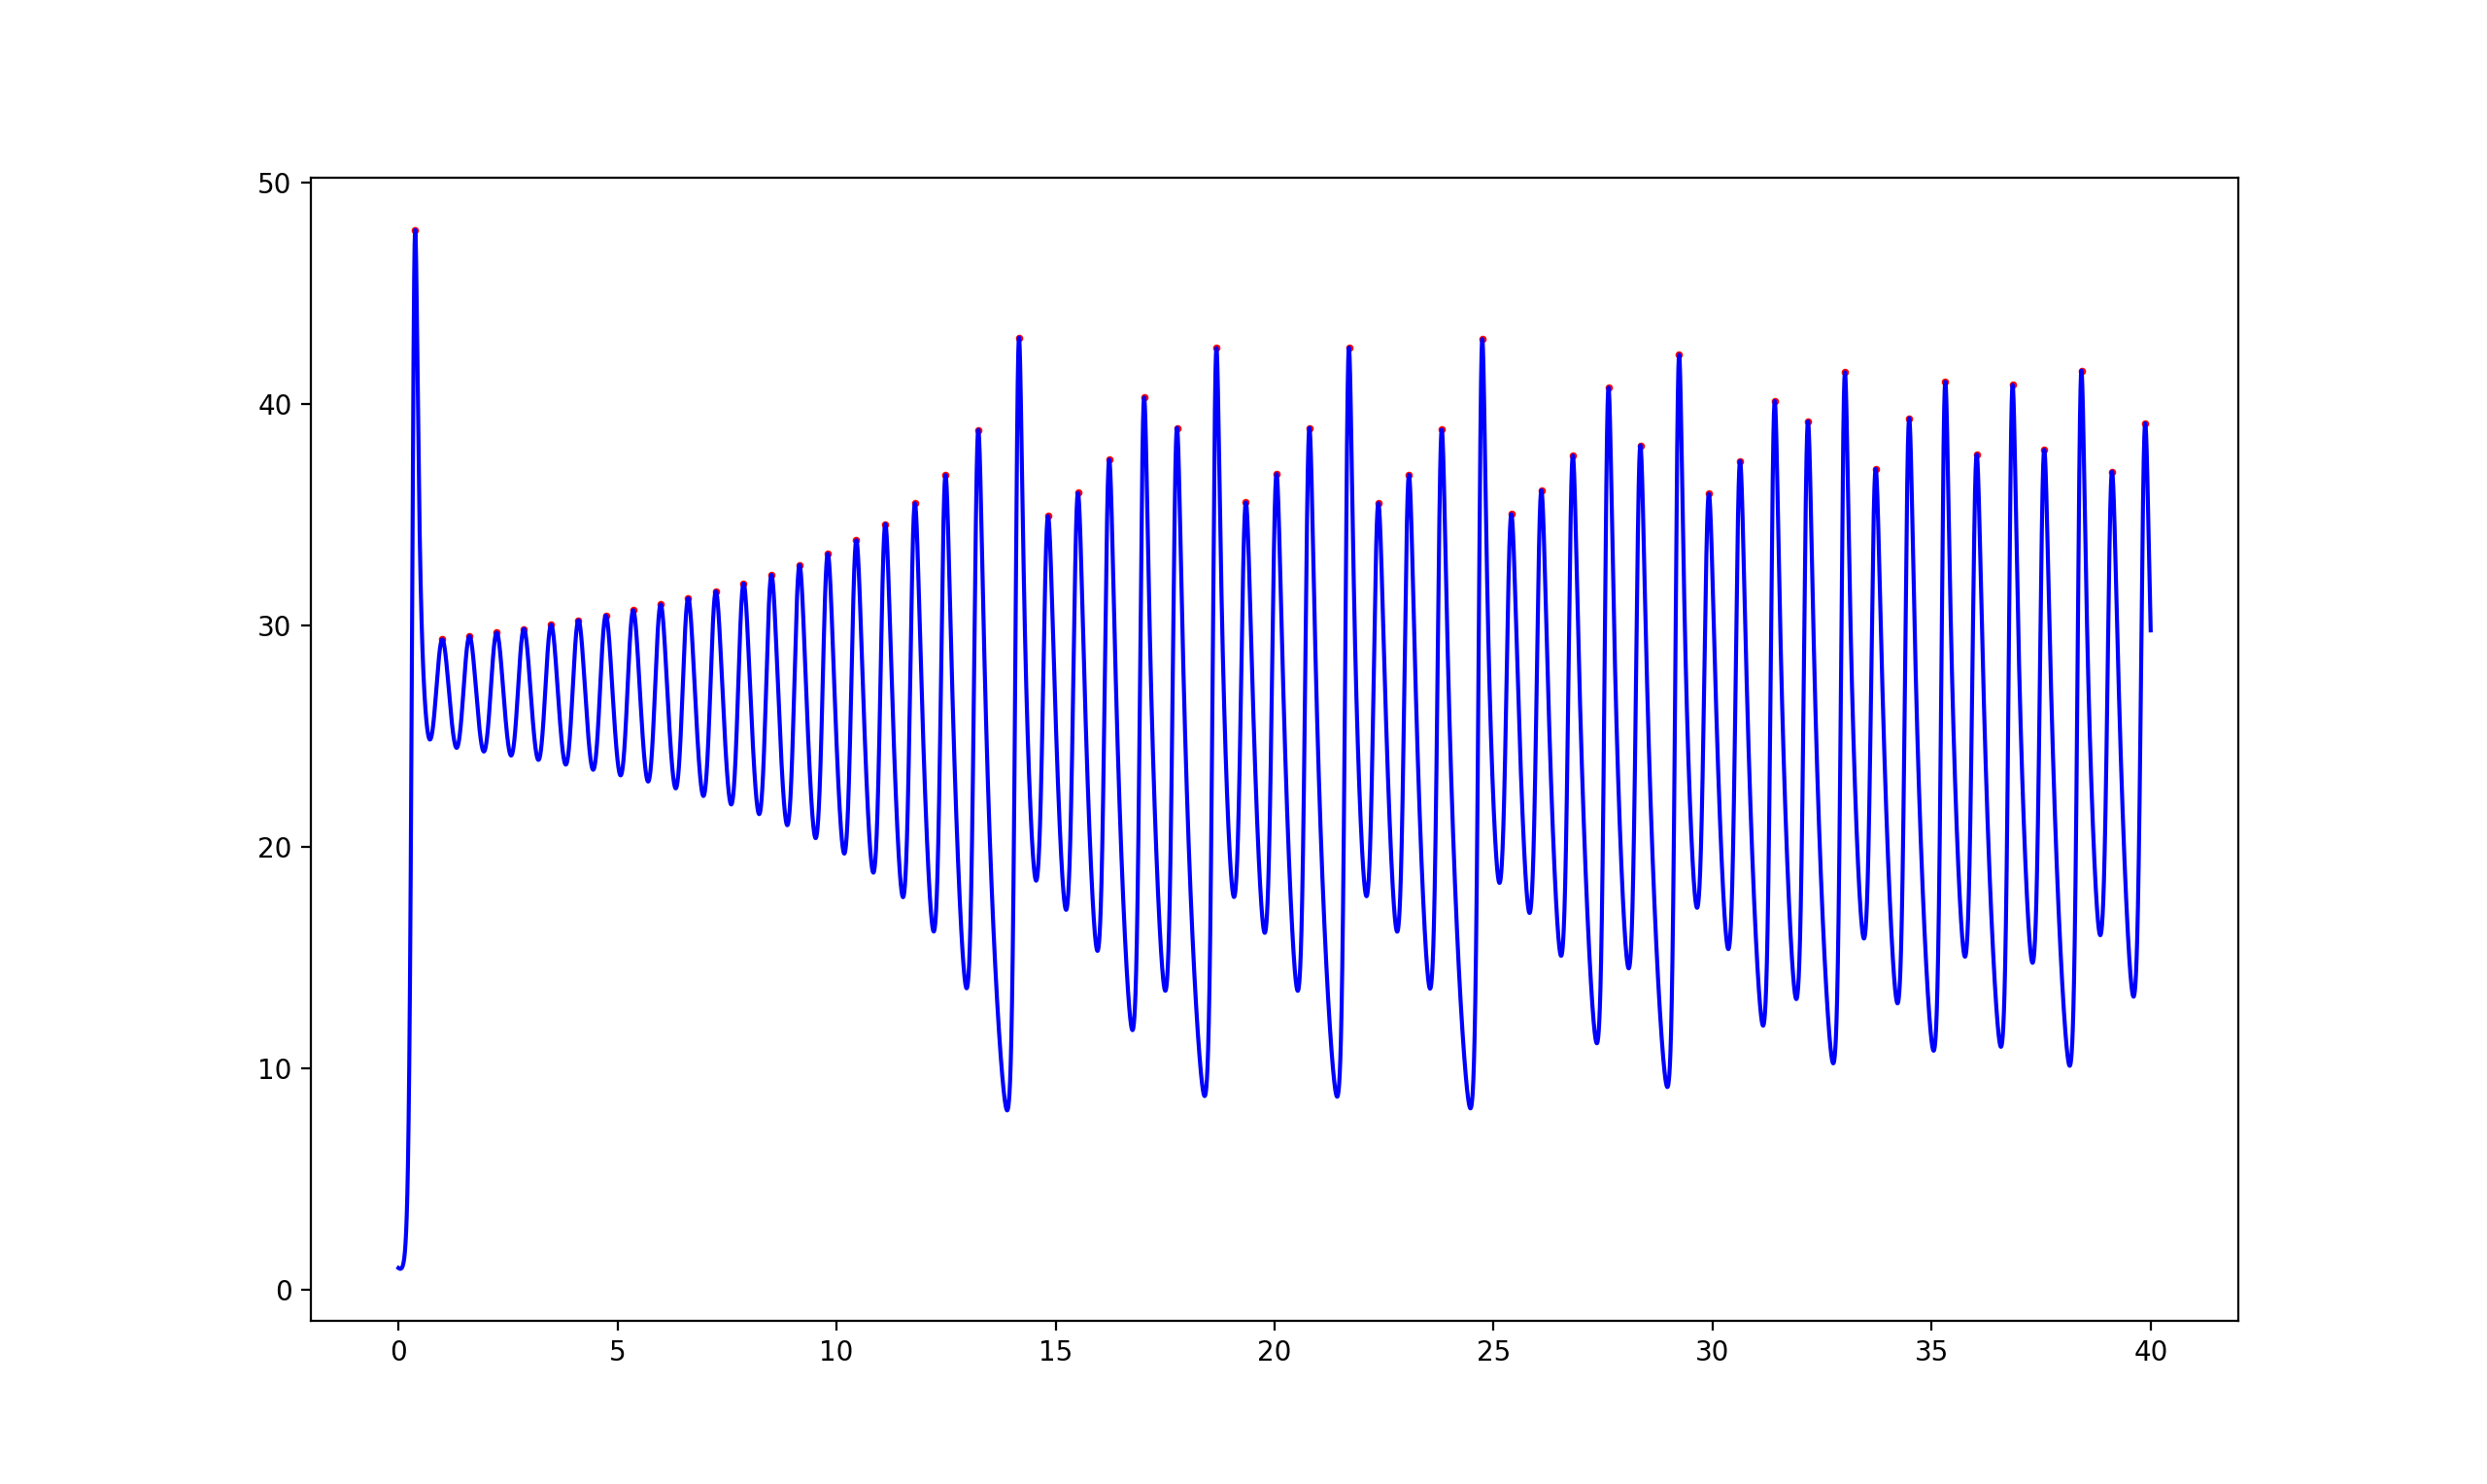
\includegraphics[width=\textwidth]{figure/section2/Lorenz-z-t.png}
\end{minipage}
\begin{minipage}[c][0.29\width]{0.29\textwidth}
   \centering
   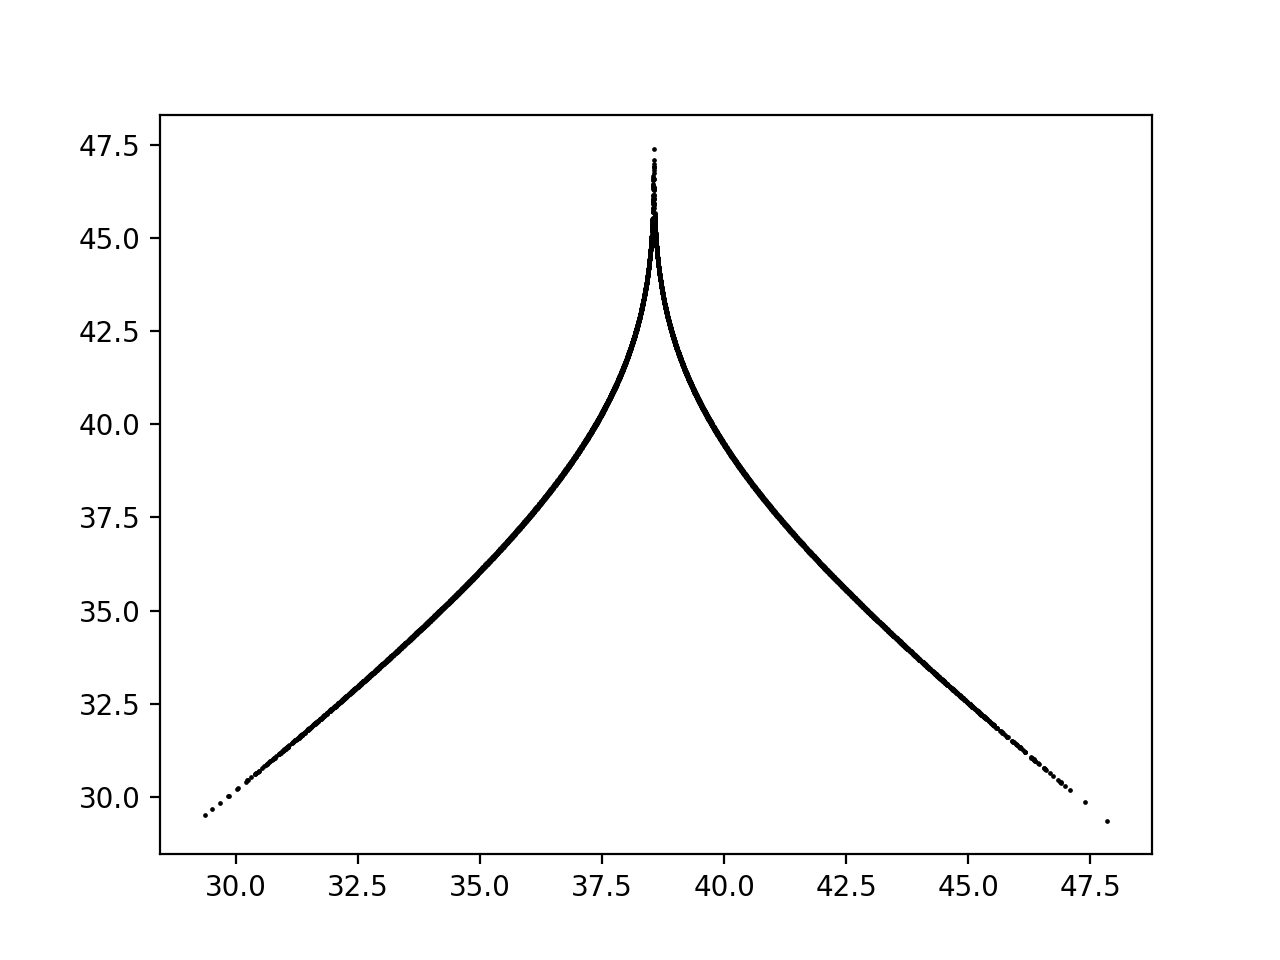
\includegraphics[width=\textwidth]{figure/section2/Lorenz-map.png}
\end{minipage}
\\[3ex]\caption{Lorenz system, $z-t$ map and Lorenz map}\label{Lorenz-map}
\end{figure}


No we consider the problem in one dimension. In the second part of Fig. \ref{Lorenz-map}, we plot the z-t figure of Lorenz model. 

Ok, we found that it is still difficult to discribe the $z-t$ figure. However, after the discussion of the logistic map $g(x) = 4x(1-x)$ as well as chaotic orbit, we know in most situation, we just care about the boundary of interval of a map. On the other hand, we found that the $z-t$ figure of Lorenz system is familiar with sine function, it is shaking during the time iteration. So if we just consider the maxinum (or the mininum) of this $z-t$ map, we can analysis the problem easier.




\begin{definition}\textbf{Lorenz map}
\\\noindent The function $z_{n+1} = f(z_n)$ satisfied the last of Fig. \ref{Lorenz-map} is called the Lorenz map. The map can be discribed in following steps.
\\\noindent \textbf{[i]} Find the $z-t$ function in Lorenz model.
\\\noindent \textbf{[ii]} The map $\{z_n\}$ is a point set which is the maxima of $z-t$ function. $z_{n+1} = f(z_n)$ where $z_{n}$ is a maxima point of $z-t$ function and $z_{n+1}$ is next maxima point of the function with growing of $t$.
\end{definition}




* The graph of Lorenz map is not actually a curve. It does have some trickness because it is not a well-defined function. However trickness is so small and there is so much to be gained by treating the graph as a curve, that we will simplt make this approximation keeping in mind that the sunsequence analysis is plausible.


%** By the way, the Lorenz map is also a kind of Poincare map.\footnote{Reference: Nonlinear Dynamics and Chaos With Applications to Physics, Biology, Chemistry, and Engineering, Steven H. Strogatz, Section 9.4, ISBN-13: 978-0813349107}


%\begin{definition}\textbf{Poincare map}
%\\\noindent The Poincare map $P$ is a mapping from $S\subset R^m$ to itself, obtained by following tarjectories from one intersection with $S$ to the next. If $x_n \in S$ denotes the k-th intersection, thne the Poincare map is defined by 
%$$
%x_{n+1} = P(x_n)
%$$ 

%Futhermore, if $x_0$ is a fixed point i.e. $P(x_0) = x_0$, then a tarjectory staring at $x_0$ returens to $x_0$ after time $T$ and is therefore a closed orbit for the original system ${dX_i\over dt} = F_i(X_1, X_2, \ldots X_m), i = 1, 2, \ldots m$
%\end{definition}



%\footnote{Hénon, M., 2021. A two-dimensional mapping with a strange attractor.}. And this is Henon's map.

As Lorenz map have no formula to discribe, it is very difficult to research that. However, in Lorenz's paper, he gave a correspondence to analysis the map, called tent map, which we has been introduced in the section 1
$$
x_{n+1} = \left\{
\begin{array}{ll}
2x_n                & x_n < {1/2} \\
\text{Undefined}    & x_n = {1/2} \\
2 - 2x_n            & x_n > {1/2}
\end{array}
\right.
$$

At least this is a piecewise continuous funcion with one discontinuous point $x = 1/2$. So we found the property of this map is not good enough to analysis. We hope the function is continuous in all domain. And we found if we try to remove this discontinuous point, then the $f'$ will satisfy $f'^{+}(1/2) = f'^{-}(1/2) = 1$. We found it is similar to the Logistic model and it seems we can discuss the property of Logistic map rather than Lorenz map. And we will explain why we can discuss the Logistic map instead of Lorenz map.

On the other hand, we found the Henon map also familiar with Logistic map in Fig. \ref{attractor-Henon-map}. The only different between Henon map and Logistic map is Henon map is fat and Logistic is thin, or a line. However if we change our parameter, like $b \rightarrow 0$, then we found \\[4ex]


\begin{figure}[H]
\begin{minipage}[c][0.32\width]{0.32\textwidth}
   \centering
   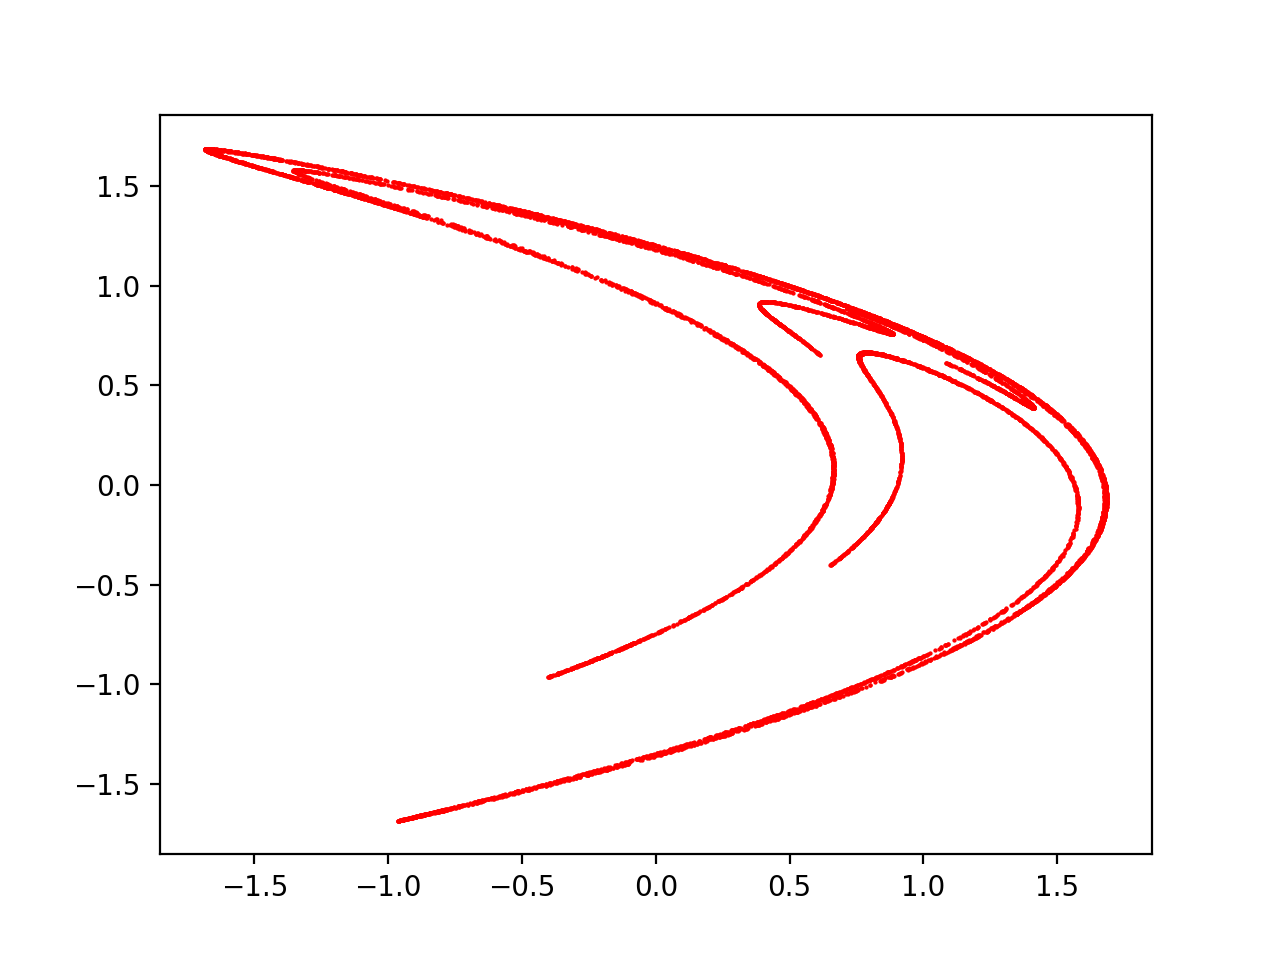
\includegraphics[width=\textwidth]{figure/section2/Henon-attractor-1*2-0*4.png}
\end{minipage}
\begin{minipage}[c][0.32\width]{0.32\textwidth}
   \centering
   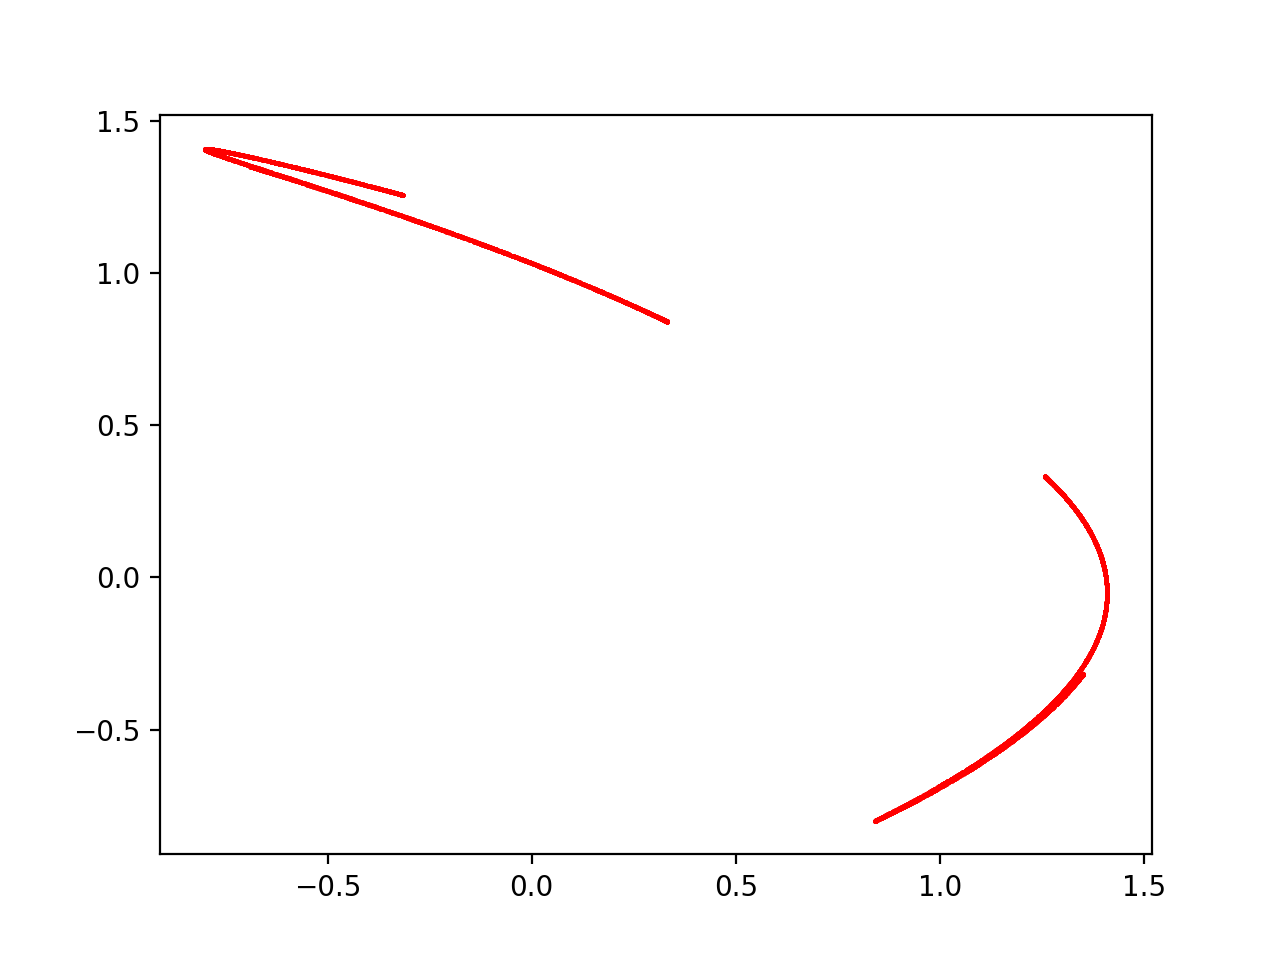
\includegraphics[width=\textwidth]{figure/section2/Henon-attractor-1*2-0*2.png}
\end{minipage}
\begin{minipage}[c][0.32\width]{0.32\textwidth}
   \centering
   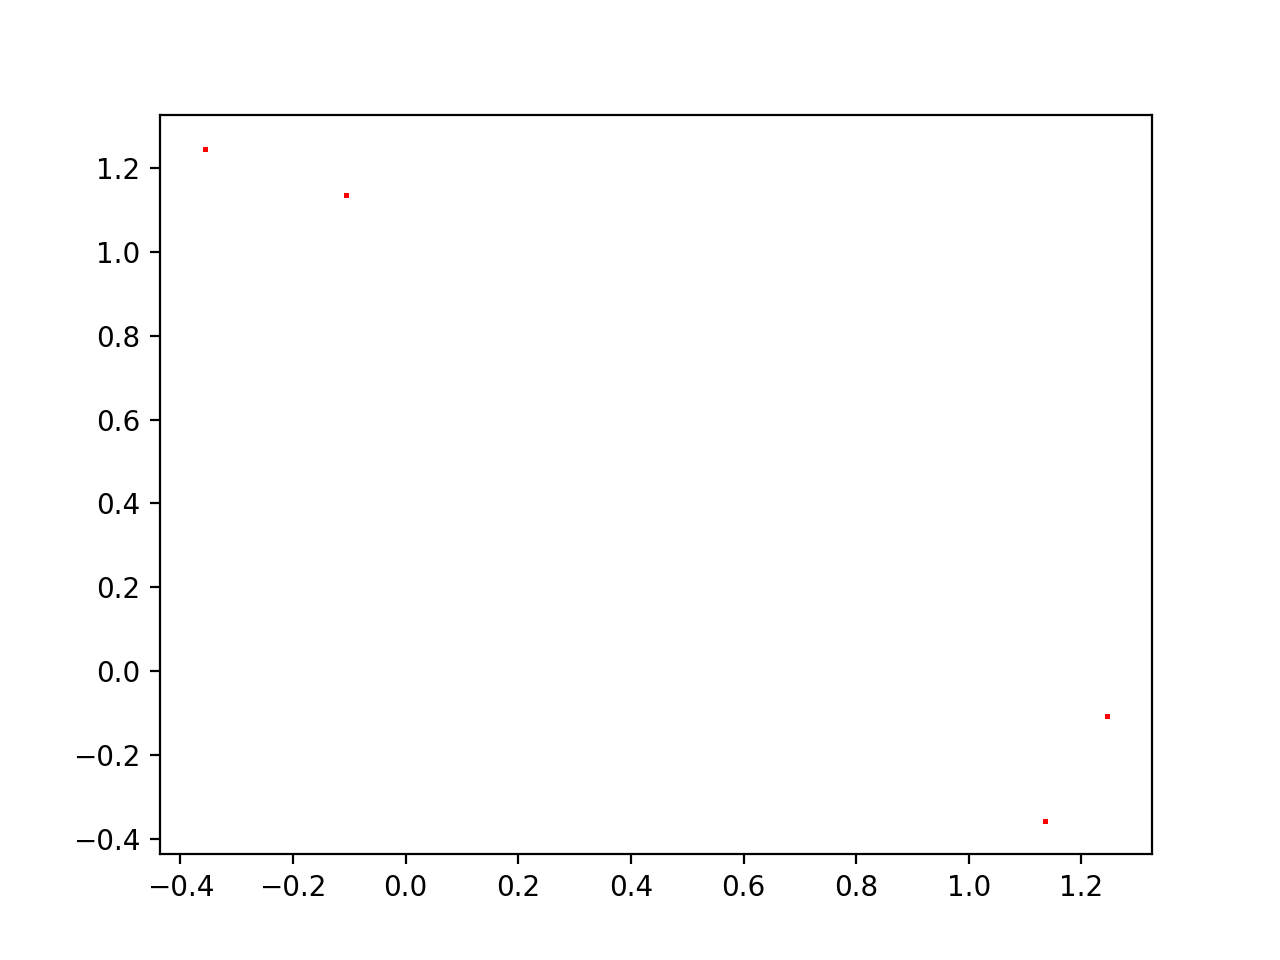
\includegraphics[width=\textwidth]{figure/section2/Henon-attractor-1*2-0*05.png}
\end{minipage}
\\[3ex]\caption{Attractor of Henon map in different $b$(0.4, 0.2, 0.05)}\label{Henon-map-b}
\end{figure}



So it \textbf{seems} we can analysis the Henon map instead of Lorenz map. But we still need more proof and in this section, we will try to solve these problems.



\end{discussion}












\subsection{Lyapunov exponents and Conjugacy}

\begin{definition} \textbf{Asymptotically periodic}
\\\noindent Consider map $f \in C^1(R^1)$. An orbit $\{x_1, x_2, \ldots x_n, \ldots\}$ is called asymptotically periodic if it convergence to a periodic orbit as $n \rightarrow \infty$, that means, $\exists \{y_1, y_2, \ldots y_k, y_1, y_2, \ldots y_km ,\ldots\}$ is a periodic orbit s.t.
$$
\lim_{n \rightarrow \infty} |x_n - y_n| = 0
$$
Also, wecalled these map as \textbf{eventually periodic} beacause their orbit is eventually lands on a periodic orbit.
\end{definition} 

For instance, the Lorenz map is a eventually periodic map. Because we found in the begining of the iteration, the map shaking in a wild interation (Just as 1-15 iterates in Fig. \ref{Lorenz-map}, second image) and after this period, the map become stable and it is convergent to the map in the 3rd image of Fig. \ref{Lorenz-map}, which we called that Lorenz map.\\[4ex]


\begin{figure}[H]
\begin{minipage}[c][0.29\width]{0.29\textwidth}
   \centering
   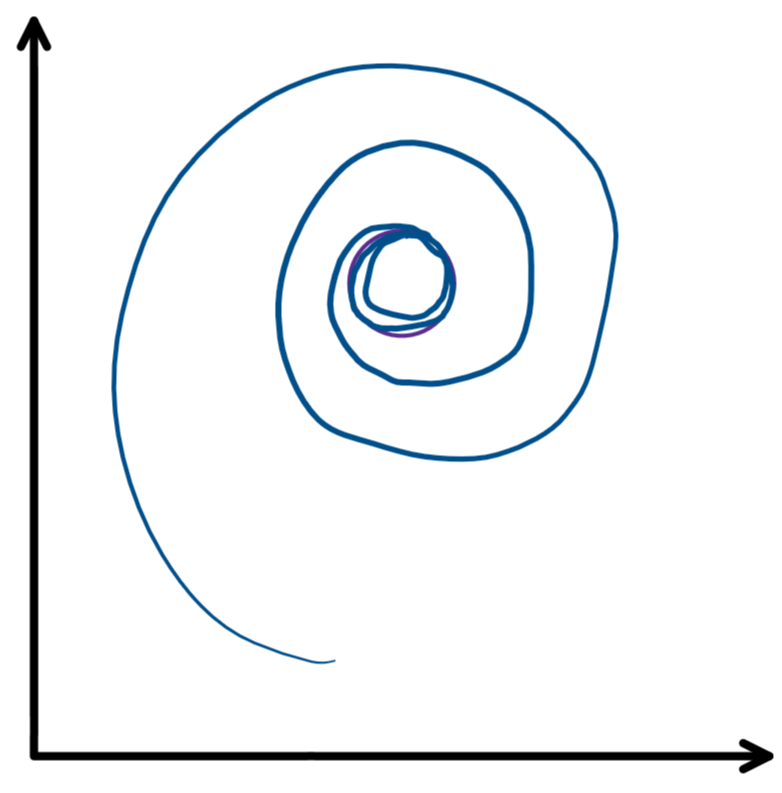
\includegraphics[width=0.7\textwidth]{figure/section3/asymptotically-periodic.png}
\end{minipage}
\begin{minipage}[c][0.4\width]{0.4\textwidth}
   \centering
   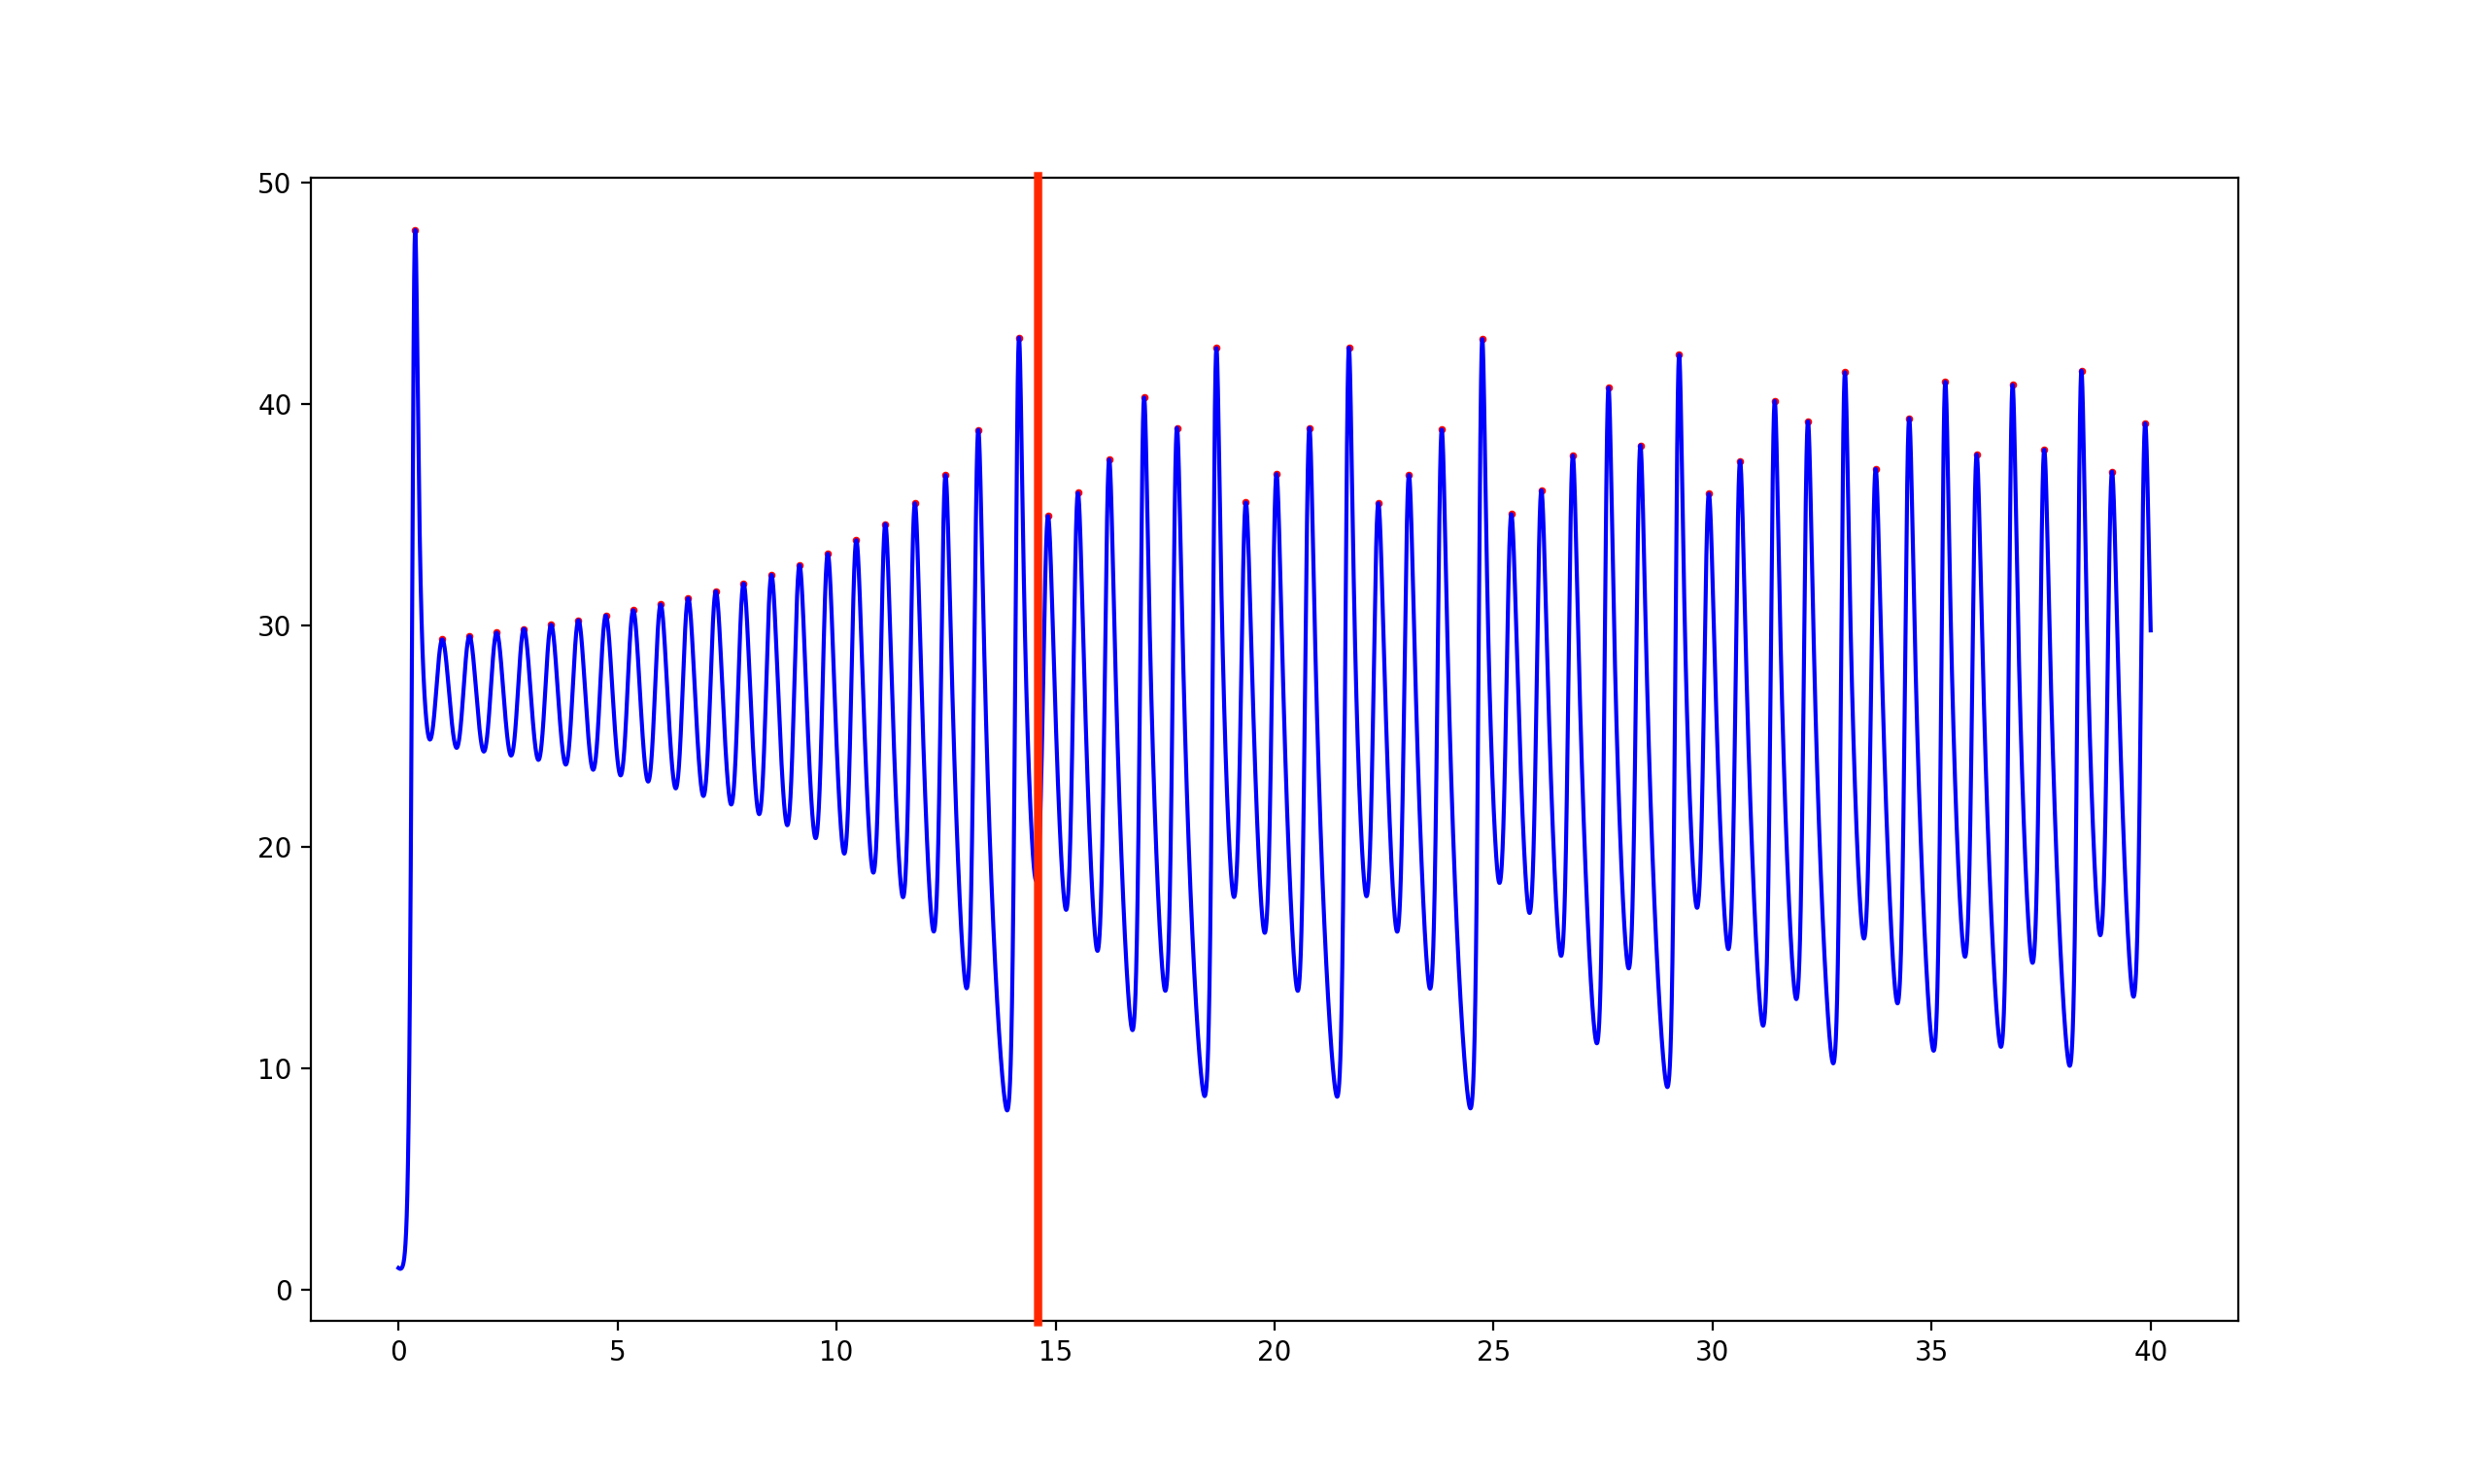
\includegraphics[width=\textwidth]{figure/section3/Lorenz-map.png}
\end{minipage}
\\[3ex]\caption{Asymptotically periodic, intro and example in Lorenz map}\label{Asymptotically-periodic}
\end{figure}

\newpage



There are several other maps with this property, for example, in section 1, we introduced the Logistic map $G(x) = 4x(1-x)$, with the initial condition $x_0 = 1/2$, we found after 2 iterates, is coincides with the fixed point $x = 0$.

Now we try to find a method to judge a map is asymptotically periodic to another periodic map. In the section 1, we introduced the stability test for periodic orbits (Theo. \ref{stability-test-for-periodic-orbits}), we called the limitation of value in Theo. \ref{chain-rule-period-orbit} as \textbf{Lyapunov number}.

\begin{definition} \textbf{Lyapunov number and Lyapunov exponent}
\\\noindent Consider map $f \in C^1(R^1)$. Define \textbf{Lyapunov number} $L(x_1)$ as 
$$
L(x_1) = \lim_{n \rightarrow \infty}(\prod_{i = 1}^{n} |f'(x_i)|)^{1/n}
$$
and based on the logarithm function, we can define the Lyapunov exponent as
$$
h_f(x_1) = h(x_1) = \lim_{n \rightarrow \infty}{1\over n}\left[\sum_{i = 1}^{n} \ln(f'(x_i))\right]
$$
Notice that $h$ exists if and only if $L$ exists and is nonzero, also $\ln L = h$. 
\end{definition} 

\begin{discussion}\label{Lyapunov-exp-discussion} \textbf{Why are we interested in Lyapunov exponent?}
\\\noindent We know that chaos means if two initial values have small different, then after long time iteration, the system showed us very different property with these two initial valus.(Just like Fig. \ref{periodic-2-check}, the error from computer results very different value, one is periodic and the other is chaos.)
\\\noindent Consider a self map $f$ and a orbit $x_0, x_1, \ldots x_n, \ldots$, where $x_{i+1} = f(x_i) = f^{i}(x_0) (\forall i \in \mathcal N)$. Now we focus on the point $x_0 + \delta_0$ where $\delta_0$ is small almost near the $x_0$ point. For other $\delta_i, i \in \mathcal N^+$, we define 
$$
\delta_i = f(x_{i-1} + \delta_{i-1}) - x_i = f^i(x_0 + \delta_0) - f^i(x_0)
$$
which discribed the distant between different initial value in $i$-iterate.
\\\noindent Based on the definition of \textbf{exponentially stable}, we assume  
$$
|\delta_i| = \exp(\lambda i)|\delta_0|
$$
then, for every $i \in \mathcal N$ which is positive, the monotony of $\exp(\lambda i)|\delta_0|$ is decided by $\lambda$. If $\lambda > 1$, the sequence $\{\delta_i\}$ is disconvergence and if $\lambda < \in (0, 1)$ the sequence is convergence. 

On the other hand, to find property of $\lambda$ is difficult beacause we cannot discribe the proprety of $\lambda$ directly. However, during the iteration, we will find every $x_1, x_2, \ldots x_n, \ldots$ as well as $\delta_1, \delta_2, \ldots, \delta_n, \ldots$, and we know that 
$$
\lambda = {1\over n}\ln{\left|\delta_n \over \delta_0\right|} 
= {1\over n}\ln{\left|f^n(x_0 + \delta_0) - f^n(x_0) \over \delta_0\right|}
$$
Based on our thought, we need $\delta_0 \rightarrow 0$ and $n \rightarrow \infty$ so
$$
\lambda = \lim_{n\rightarrow \infty}{1\over n}\ln{\left|\lim_{\delta_0 \rightarrow 0}\left(f^n(x_0 + \delta_0) - f^n(x_0) \over \delta_0\right)\right|} 
= \lim_{n\rightarrow \infty}{1\over n}\ln{\left|(f^n)'(x_0)\right|} 
= \lim_{n\rightarrow \infty}{1\over n}\ln{\left|\prod_{i = 0}^{n}f'(x_i)\right|} 
$$
which is the definition of Lyapunov number.
\end{discussion}


Based on this Lyapunov exponent, we have this theorem.
\begin{theorem}\label{Lyapunov-exponent-asymptotically-periodic} Consider map $f \in C^1(R^1)$. If orbits $\{x_1, x_2, \ldots\}$ of $f$ satisfies $f'(x_i) \neq 0 \forall i \in N$ and it is asymptotically periodic to the periodic orbit ${y_1, y_2, \ldots}$, then two orbit have indentical Lyapunov exponents, assuming both exist.
\end{theorem}


{\color{blue}
\begin{proof}\textbf{[i]} If we consider a sequence $\{s_i\}$ s.t. $\lim_{i \rightarrow \infty0} s_i = s$, then 
$$
\forall \varepsilon > 0, \exists N_1 \in \mathcal N \text{ s.t. } \forall n > N_1, |s_n - s| < \varepsilon
$$
Now we consider the average of $\{s_i\}$, we found for this $\varepsilon$,
$$
\lim_{N \rightarrow \infty}{1 \over N}\left|\sum_{i = 1}^{N}s_i - s\right| 
= \lim_{N \rightarrow \infty} {1\over N}\sum_{i = 1}^{N}\left|s_i - s\right| 
= \lim_{N \rightarrow \infty} {1\over N}\left[\sum_{i = 1}^{N_1 - 1}\left|s_i - s\right| + \sum_{i = N_1}^{N}\left|s_i - s\right|\right] 
$$
$$
= \lim_{N \rightarrow \infty} {1\over N}\sum_{i = 1}^{N_1 - 1}\left|s_i - s\right| + \lim_{N \rightarrow \infty}{1\over N}\sum_{i = N_1}^{N}\left|s_i - s\right| 
\leq 0 + \lim_{N \rightarrow \infty}{1\over N - N_1}\sum_{i = N_1}^{N}\left|s_i - s\right|
< {N 0 N_1\over N - N_1}\varepsilon = \varepsilon 
$$
So we have this conclusion
$$
\forall \varepsilon > 0, \exists N_1 \in \mathcal N, \text{ s.t. } \forall n > N_1, \lim_{N \rightarrow \infty}{1 \over N}\left|\sum_{i = 1}^{N}s_i - s\right| < \varepsilon \Rightarrow \lim_{N \rightarrow \infty}{1\over N}\sum_{i =1}^{N}s_i = s
$$

  \noindent \textbf{[ii]} Let $y_1$ is the fixed point (that means, $x_i$ asymptotically periodic to a periodic-1 orbit), then $\lim_{n \rightarrow \infty} x_n = y_1$. As $f \in C^1(R^1)$, then $f'$ is exists and $f'$ Riemann integrable (and of course, Lebesgue integrable), so we can exchange the order of integral(or differential of $f$) and limitation, then we have
$$
\lim_{n \rightarrow \infty}f'(x_n) = f'(\lim_{n \rightarrow \infty} x_n) = f'(y_1)
$$
On the other hand, as $\ln|x|$ is a continuous, monotony function for $x \in R^+$, then 
$$
\lim_{n\rightarrow \infty} \ln |f'(x_n)| = \ln \left|\lim_{n\rightarrow \infty}f'(x_n)\right| = \ln |f'(y_1)| 
\Rightarrow h(x_1) = \lim_{n \rightarrow \infty}{1\over n}\sum_{i = 1}^{n} \ln |f'(x_i)| = \ln|f'(y_1)| = h(y_1)
$$
            \textbf{[iii]} Now we assume $k > 1, k \in \mathcal N$, obviously, $y_1$ is fixed point of $f^k$, and 
$$
h_{f^k}(x_1) = \ln |(f^k)'(y_1)| = h_{f^k}(y_1)
$$
            Now we will prove $h_{f^k}(x_1) = {1\over k} h_{f}(x_1)$. Based on the definition, we know
$$
h_{f^k}(x_1) = \lim_{n \rightarrow \infty}{1 \over n} \sum_{i = 1}^{n}\ln\left|(f^k)'(x_i)\right| 
= \lim_{n \rightarrow \infty}{1 \over n} \sum_{i = 1}^{n}\ln\left|{1\over k}\prod_{j = i}^{i + k}f'(x_i)\right| 
= {1\over k}\lim_{n \rightarrow \infty}{1 \over n} \sum_{i = 1}^{n}\sum_{j = i}^{i + k}\ln\left|f'(x_i)\right| 
= {1 \over k} h_f(x_1)
$$
            And we proved the theorem. $\blacksquare$
\end{proof}
}


\begin{figure}[H]
\begin{center}
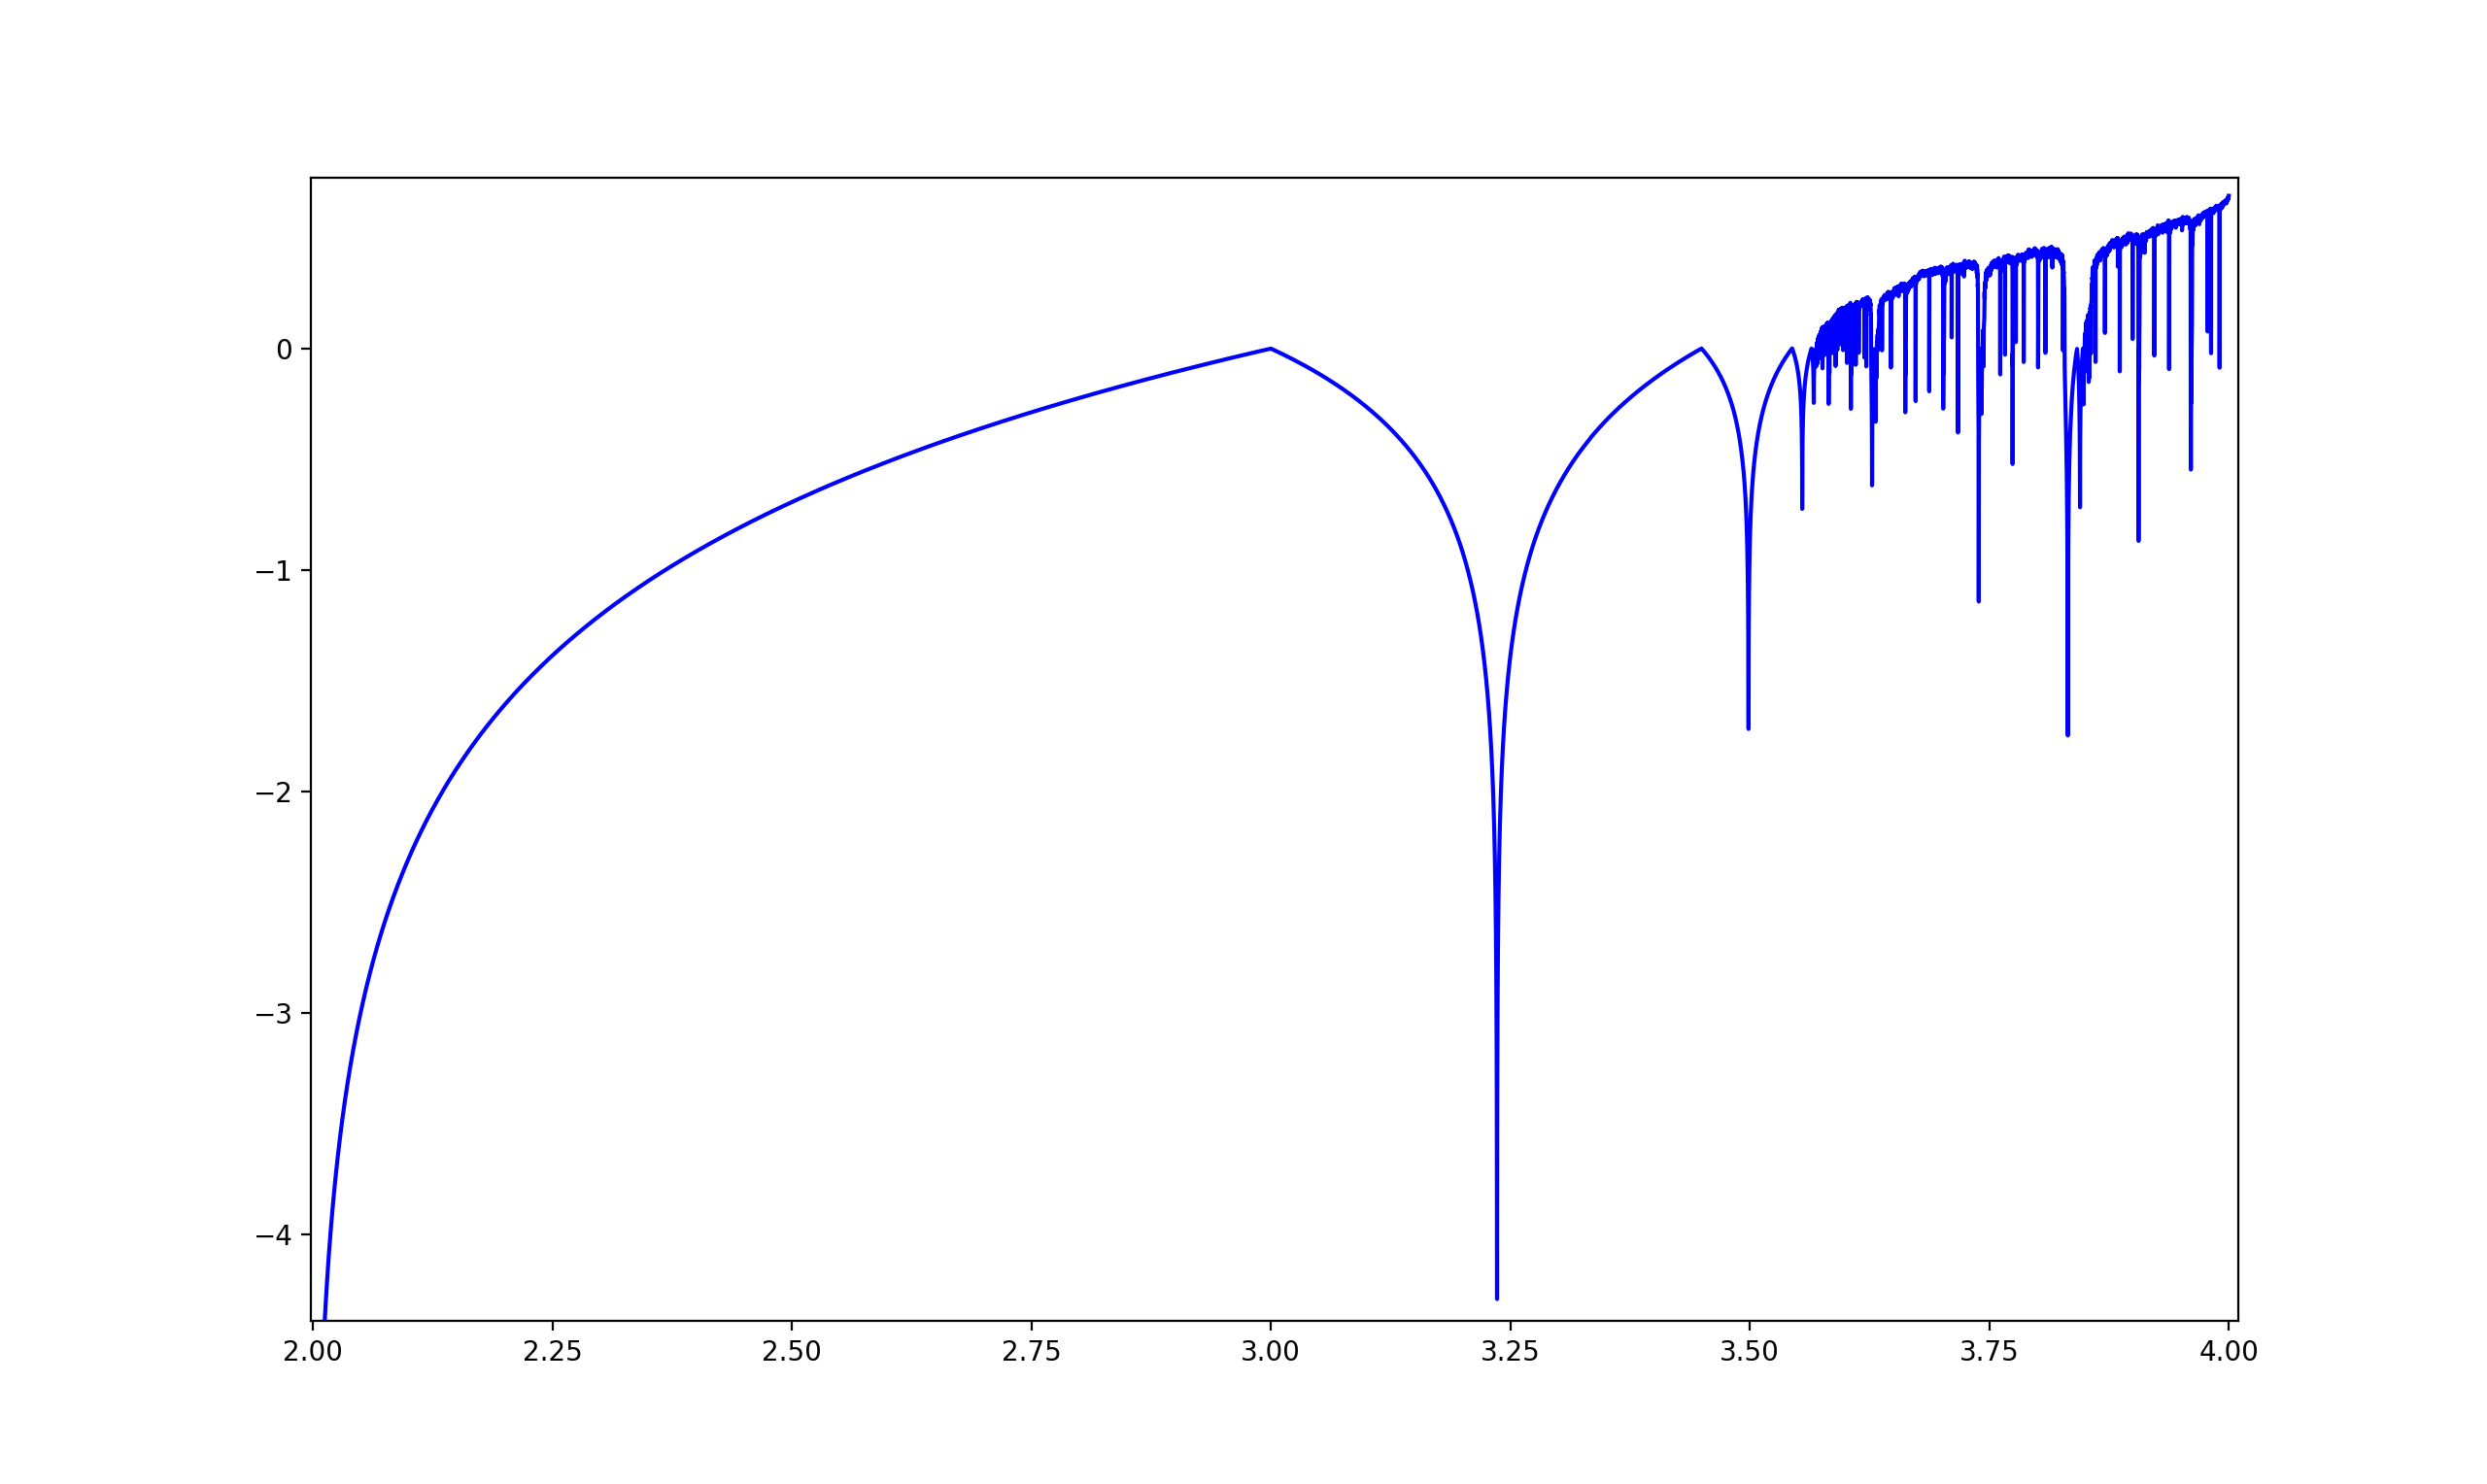
\includegraphics[width=0.5\textwidth]{figure/section3/logistic-lyapunov-exp.png} \\
\caption{Lyapunov exponent of logistic model in different parameter}\label{logistic-lyapunov-exp}
\end{center}
\end{figure}


Obviously, the chaotic orbit satisfied Def. \ref{chaos-orbit} will have no asymptotically periodic and we have this theorem.


\begin{definition}\label{Lyapunov-exponent-chaotic} Consider map $f \in C^1(R^1)$, the orbit is \textbf{chaotic} if it satisfied both
\\\noindent \textbf{[i]} $\{x_1, x_2, \ldots \}$ is no asymptotically periodic, and
\\\noindent \textbf{[ii]} the Lyapunov exponent $h(x_1)$ is \textbf{greater} than zero.
\end{definition}









Now we will discuss the mod map and the tent map.

The mod map has been introduced in section 1 (Fig. \ref{3xmod1}) and we will mainly discuss the $f(x) = 2x (mod 1)$ in this discussion. A simple way to analysis the stability of map is itinerary.\\[3ex]



\begin{figure}[H]
\begin{minipage}[c][0.24\width]{0.24\textwidth}
   \centering
   \includegraphics[width=\textwidth]{figure/section3/mod2-ite1.png}
\end{minipage}
\begin{minipage}[c][0.24\width]{0.24\textwidth}
   \centering
   \includegraphics[width=\textwidth]{figure/section3/mod2-ite2.png}
\end{minipage}
\begin{minipage}[c][0.24\width]{0.24\textwidth}
   \centering
   \includegraphics[width=\textwidth]{figure/section3/mod2-ite3.png}
\end{minipage}
\begin{minipage}[c][0.24\width]{0.24\textwidth}
   \centering
   \includegraphics[width=\textwidth]{figure/section3/mod2-itinerary.png}
\end{minipage}
\\[3ex]\caption{Iterates and itinerary of mod-2 map}\label{mod-2-map}
\end{figure}


\textbf{[i] Binary and itinerary of mod map}
\\\noindent We will focus on the initial value $0.2$ of mod-2 map firstly. That is simple to find the itinerary with the code we used in section 1.

\begin{table}[H]
\centering  
\caption{Logistic4 itinerary with different initial value}  
\begin{tabular}{|c||l|l|l|l|l|}
\hline
Val  & $1-8$              & $9-16$             & $17-24$             & $25-32$             & $\ldots$ \\
\hline
0.2 & \textbf{LLRRLLRR} & \textbf{LLRRLLRR} & \textbf{LLRRLLRR} & \textbf{LLRRLLRR} & $\ldots$ \\
\hline
\end{tabular}  
\end{table}

We found that this point is a periodic-4 point. And now, to analysis the problem simple, we will import a new method based on the binary number. In this problem, we have
$$
{1\over 5} = 0.\overline{0011}, \ \ \ \ f({1\over 5}) = 0.011\overline{0011}, \ \ \ \ f^2({1\over 5}) = 0.11\overline{0011}, \ \ \ \ f^3({1\over 5}) = 0.1\overline{0011}, \ \ \ \ f^4({1\over 5}) = \overline{0011}, \ \ \ \ 
$$
and obviously $1/5$ point is a periodic-4 orbit. So in summary, we can use binary value to find the period of every point in this map.

Now we consider the Lyapunov exponent of mod map. Obviously, the differential of map is equal to 2 except the discontinuous point $1/2$, so for ever initial value different from the $1/2$, we have
$$
h_{mod-2}(x_1) = \lim_{n \rightarrow \infty}{1\over n}\left[\sum_{i = 1}^{n}\ln\left(f'(x_i)\right)\right] = \lim_{n \rightarrow \infty}{1\over n}\left[\sum_{i = 1}^{n} \ln(2)\right] = \lim_{n \rightarrow \infty}\left({1 \over n} n \ln(2)\right) = \ln(2) > 0
$$
So the conclusion is the orbit of every initial value will result chaotic.\\[2ex]




\textbf{[ii] Mod-Sum model and asymptotically periodic}

Now we change the mod model a little bit.
$$
f(x) = (x + q)(mod 1) \text{ where } q \text{ is a constant.}
$$
We will mainly consider the $q \in [0, 1]$, if not, $\exists p \in [0, 1]$ and $p = q(mod 1) \land \forall x \in [0, 1] f_q(x) = (x+q)(mod 1) = f_p(x) = (x+p)(mod 1)$.

That is simple to found the discontinuous point of $f_q(x)$ as $1 - q$, futhermore, the differential of model is equal to $1$ except this discontinuous point. So we have the Lyapunov exponent as 
$$
h_{f_q}(x_1) = \lim_{n \rightarrow \infty}{1\over n}\left[\sum_{i = 1}^{n}\ln\left(f'(x_i)\right)\right] = \lim_{n \rightarrow \infty}{1\over n}\left[\sum_{i = 1}^{n} \ln(1)\right] = 0
$$
And\\[2ex]







\textbf{[iii] Tent map}
Now we consider the tent map. 
\begin{figure}[H]
\begin{center}
\includegraphics[width=1\textwidth]{figure/section3/tent-map.png} \\
\caption{Tent map}\label{tent-map}
\end{center}
\end{figure}

We found that tent map have similar property of mod-2 map, that is because of the left side of the tent map is equal to the mod-2 map, and the right side of the tent map is symmetric of mod-2 map. So we can found that the size of interval in itinerary of both mod-2 map and tent map are $2^{k}$ and the only different between the mod-2 map and tent map is tent map will exchange the order of the \textbf{L} and \textbf{R} during iteration. 

However, if we consider the topic of asymptotically periodic, we can found this conclusion.

\begin{theorem} The tent map $T$ has infinitely many chaotic orbits.
\end{theorem}

{\color{blue}
\begin{proof} \textbf{[i]}Consider the set of $[0, 1]\backslash Q$ which is combined with all irrational number in $[0, 1]$. If $x \in [0, 1]\backslash Q$, then
\\\noindent \textbf{1.} If $x < 1/2$, then $x_{new} = 2x \in [0, 1]\backslash Q$
\\\noindent \textbf{2.} If $x > 1/2$, then $x_{new} = 2 - 2x \in [0, 1]\backslash Q$
\\\noindent Now we consider a orbit with irrational begining, obviously, every value of this orbit is based on irrational value. And we know that there are infinity element in $[0, 1]\backslash Q$, so we have infinity irrational based orbits.\\[1ex]

  \noindent On the other hand, we know ever orbits avoid have
$$
\forall x_1 \in [0, 1], x_1 \neq {1\over 2}, h_{f}(x_1) = \lim_{n \rightarrow \infty}{1\over n}\left[\sum_{i = 1}^{n}\ln\left|f'(x_i)\right|\right] = \lim_{n \rightarrow \infty}{1\over n}\left[\sum_{i = 1}^{n} \ln(2)\right] = \ln(2) > 0
$$
As $1/2$ is a rational value, so every orbit in \textbf{[i]} will avoid this point. So all of these orbits are chaotic. And in summary we found infinity many chaotic orbits in tent map T. $\blacksquare$
\end{proof}
}








\textbf{[iv] Conjugacy and Logistic map}

First of all, we will list the main property in both logistic-4 map and tent map.

\begin{table}[H]
\centering  
\caption{Logistic-4 map VS tent map}  
\begin{tabular}{|c||c|c|}
\hline
Property             & Logistic-4 map($G(x)$)  & Tent map($T(x)$) \\
\hline
\hline
Critical point       & \multicolumn{2}{c|}{$1/2 \rightarrow 1 \rightarrow 0$}\\
\hline
Fixed point          & $0, 3/4$ & $0, 2/3$ \\
\hline
Period-2 orbit       & $\{(5-\sqrt5)/8, (5+\sqrt5)/8\}$ (Single) & $\{0.4, 0.8\}$ (Single) \\
                     & \multicolumn{2}{c|}{Lies in the same relation, one in $[0, 1/2]$ and the other in $[1/2, 1]$} \\
                     & \multicolumn{2}{c|}{where $1/2$ is critical point} \\
\hline
\end{tabular}  
\end{table}  

We will check the derivative value for periodic-k orbit in both map.
\\\noindent \textbf{Periodic-1}
\\\noindent \textbf{[1] Tent map} $T'(2/3) = -2$
\\\noindent \textbf{[2] Logistic map} $G'(3/4) = -2$
\\\noindent CONCLUSION: $T'(2/3) = G'(3/4)$
\\\noindent \textbf{Periodic-2}
\\\noindent \textbf{[1] Tent map} $T'(0.4)T'(0.8) = -4$
\\\noindent \textbf{[2] Logistic map} $T'((5-\sqrt5)/8)T'((5+\sqrt5)/8) = -4$
\\\noindent CONCLUSION: $T'(0.4)T'(0.8) = T'((5-\sqrt5)/8)T'((5+\sqrt5)/8) = -4 = -2^2$
\\\noindent $\ldots$

We found some intersted result, but we cannot confirm how long these property still established. To solve, or to prove the similiarity of tent map and logistic map, we will import the definition of conjugate.

\begin{definition}The mape $f$ and $g$ are \textbf{conjugate} if they are related by a continuous one-to-one change of coordinates, that is, if $C \circ f = g \circ C$.
\end{definition}

\begin{problem} Proof: Map $T$ and $G$ are conjugate, and the $C$ is $C(x) = \left(1 - \cos (\pi x)\right)/2$.
\end{problem}
{\color{blue}
\begin{proof}\textbf{[i] $x \in [0, 1/2]$} $G(C(x)) = 4(C(x))(1 - C(x)) = 1 - \cos^2(\pi x) = \sin^2 (\pi x)$
\\\noindent $C(T(x)) = {1 - \cos(2\pi x)} / 2 = \sin^2(\pi x) = G(C(x))$
\\\noindent \textbf{[ii] $x \in [1/2, 1]$} $G(C(x)) = 4(C(x))(1 - C(x)) = 1 - \cos^2(\pi x) = \sin^2 (\pi x)$
\\\noindent $C(T(x)) = {1 - \cos(\pi (2 - 2x)} / 2 = {1 - \cos(2\pi x)} / 2  =\sin^2(\pi x) = G(C(x))$
\\\noindent In summary we proved the problem. $\blacksquare$
\end{proof}
}

Familiar with matrix exponent, if we consider the $G^n$ map, then
$$
G^n = G \circ G \circ G \circ G \circ \ldots \circ G = CTC^{-1}CTC^{-1}CTC^{-1}CTC^{-1} \ldots CTC^{-1} = CT^nC^{-1} \Rightarrow G^nC = CT^n
$$

\begin{theorem} If $x$ is periodic-k point of $f$, then $C(x)$ is a periodic-k point of $g$, where $f, g$ are conjugate with $C$ and $Cf = gC$. 
\end{theorem}
{\color{blue}
\begin{proof} With the conclusion above, we have
$$
f^k = C^{-1}g^kC, \text{ then } \forall x \text{ is a periodic-k point }, f^k(x) = C^{-1}\{g^k[C^{}(x)]\} = x \Rightarrow g^k[C(x)] = C(x) \blacksquare
$$
\end{proof}
}

Now we focus on the partical of map, because we want to know if the conclusion like $T'(0.4)T'(0.8) = T'((5-\sqrt5)/8)T'((5+\sqrt5)/8) = -4$ is established on high dimension or not.
\begin{theorem} If $f$ and $g$ are conjugate with $C$ and $Cf = gC$ and $x$ is periodic-k point of $f$ (that means $C(x)$ is a periodic-k point of $g$), then
$$
(g^k)'[C(x)] = (f^k)'(x)
$$ 
\end{theorem}

{\color{blue}
\begin{proof} \textbf{[1]} The chain rule says that 
$$
C[f(x)] = g[C(x)] \Rightarrow C'[f(x)]f'(x) = g'[C(x)]C'(x)
$$
If $x$ is periodic-1 (fixed) point, then $f(x) = x \land g(C(x)) = C(x)$, so we have
$$
C'(x)f'(x) = g'[C(x)]C'(x) \Rightarrow f'(x) = g'[C(x)]
$$
\\\noindent \textbf{[2]} Now if $x$ is periodic-2 point, then $f^2(x) = x, g^2[C(x)] = C(x) \land C[f^2(x)]=g^2[C(x)]$ and 
$$
{dC[f^2(x)] \over dx} 
= C'[f^2(x)]{df[f(x)] \over dx} 
= C'[x]{df[f(x)] \over dx}
={dg\{g[C(x)]\} \over dx} = [(g^2)'(C(x))]C'(x)
$$
So In summary we have
$$
(f^2)'(x) = (g^2)'(C(x))
$$
\textbf{[k]} Now we consider arbitrary $k \in \mathcal N$, familiar periodic-2, for a periodic-k point $x$, we have $f^{k}(x) = x, g{k}[C(x)] = C(x) \land C[f^{k}(x)]=g^{k}[C(x)]$ and 
$$
{d\{C[f^{k}(x)]\} \over dx} = C'[f^{k}(x)](f^{k})'(x) = C'(x)(f^{k})'(x) = {d\{(g^k)[C(x)]\} \over dx} = (g^k)'[C(x)]C'(x) 
$$
In summary we proved the conclusion that $\forall k \in \mathcal N, (f^k)'(x) = (g^k)'(C(x)) \blacksquare$
\end{proof}
}

Now we can simply found this conclusion:

\begin{conclusion} If $f$ and $g$ are conjugate with $C$ and $Cf = gC$ and $\{x_1, x_2, \ldots x_k\}$ is periodic-k orbit of $f$ (that means $\{C(x_1), C(x_2), \ldots C(x_k)\}$ is a periodic-k orbit of $g$), then 
$$
\prod_{i = 1}^{k}f'(x_i) = \prod_{i = 1}^{k}g'(C(x_i))
$$
\end{conclusion}
{\color{blue}
\begin{proof} Based on the chain rule, we still have
$$
(f^{k})'(x_1) = [f^{k-1} (f)]'(x_1) = (f^{k-1})'(f(x_1)) f'(x_1) = (f^{k-1})'(x_2) f'(x_1) = \ldots = \prod_{i = 1}^{k}f'(x_i)
$$
also this conclusion is established in $(g^k)'(C(x)) \blacksquare$
\end{proof}
}


Based on the conjugacy, we can prove these series of conclusions
\begin{conclusion} All periodic points of logistic map $G$ are source.
\end{conclusion}
{\color{blue}
\begin{proof} Firstly, we consider the tent map $T$, and obviously the point $0, 1/2$ and $1$ will now be the periodic points because they result asymptotically periodic. And for ever other point of tent map, we know that $|T'(x)| \equiv 2$. On the other hand, we know that exists $C$ s.t. $GC(x) = CT(x)$, so 
$$
\prod_{i = 1}^{k}|G'(x_i)| = \prod_{i = 1}^{k}|T'(C(x_i))| = 2^k > 1 \blacksquare
$$
(Also, this conclusion told us that $\prod_{i = 1}^{k}|G'(x_i)| = 2^k$ will always be established, which we has beed found in periodic-1 and periodic-2 discussion.)
\end{proof}
}


\begin{conclusion} Consider a itinerary figure of logistic map $G$, the length of every k-iterates subinterval is lower than $\pi \over 2^{k+1}$.
\end{conclusion}
{\color{blue}
\begin{proof} Consider a subinterval of itinerary after k-iterates $[x_p, x_q]$ where 
\\\noindent $\forall x \in [x_p, x_q], T^k(x) \text{ have symbol } \textbf{L} \lor T^k(x)\equiv\textbf{R}$ and $\forall \varepsilon > 0\forall x \in (N_\varepsilon(x_p) \bigcup  N_\varepsilon(x_q))\backslash[x_p, x_q], T^k(x) $ have different symbol of $x \in [x_p, x_q]$. Obviously, we know that $\mu([x_p, x_q]) = 2^{-k}$, where $\mu$ is lebesgue measure (or the length of the interval), then
$$
\mu_G([x_p, x_q]) = C(x_q) - C(x_p) = \int_{x_p}^{x_q}C'(x) dx = \int_{x_p}^{x_q}{\pi \over 2}\sin(\pi x) d \leq {\pi \over 2}\int_{x_p}^{x_q}dx = {\pi \over 2}(x_q - x_p) = {\pi \over 2^{k+1}} \blacksquare
$$

\end{proof}
}

\newpage
Finally, we will use the tools of Lyapunov exponent as well as conjugacy to proof the following theorem.

\begin{theorem} The logistic map $G$ has chaotic orbit.
\end{theorem}

\begin{lemma} If $f$ and $g$ are conjugate with $C$ and $Cf = gC$ 
\\\noindent $\{x_1, x_2, \ldots x_k, \ldots\} and \{C(x_1), C(x_2), \ldots C(x_k), \ldots\}$ are orbit of $f$ and $g$, if $C$ satisfied $\lim_{k \rightarrow \infty} {1\over k}C'(x_k) = 0$ then we have 
$$
h_f(x_1) = h_g(C(x_1))
$$ 
\end{lemma}



{\color{blue}
\begin{proof} Consider $C[f(x_i)] = g[C(x_i)]$, then the chain rule told us that
$$
\{C[f(x_i)]\}' = C'[f(x_i)]f'(x_i) = C'(x_{i+1})f'(x_i) = \{g[C(x_i)]\}' = g'[C(x_i)]C'(x_i) 
$$
$$\Rightarrow  f'(x_i) = g'[C(x_i)]{C'(x_i) \over C'(x_{i+1})} \Rightarrow \prod_{i = 1}^{k}f'(x_i) = \prod_{i = 1}^{k}g'(C(x_i))\left(C'{x_1} \over C'(x_{k+1})\right)
$$
(This formula obey the conclusion above, if we pay attention to the condition, we know that once $x_1$ is a periodic-k point, then $x_{k+1} = x_1$ and we have $\prod_{i = 1}^{k}f'(x_i) = \prod_{i = 1}^{k}g'(C(x_i))$) 
\\\noindent Moreover, based on the definition of Lyapunov exponent, there is
$$
\ln\left|\prod_{i = 1}^{k}f'(x_i) \right| = \sum_{i = 1}^{k}\ln\left|f'(x_i) \right| 
= \ln\left|\prod_{i = 1}^{k}g'[C(x_i)] \right| + \ln\left|C'(x_1) \right| - \ln\left|C'(x_{k+1}) \right| 
$$
Note that $C'(x_1)$ is constant so $ \lim_{k \rightarrow \infty} {1 \over k}\left(\ln\left|C'(x_1) \right| \right) = 0$. And based on the condition of theorem, we have $\lim_{k \rightarrow \infty}{1 \over k}\ln\left|C'(x_{k+1}) \right| = 0$
\\\noindent So finally 
$$
h_f(x_1) = \lim_{k \rightarrow \infty}{1\over k}\sum_{i = 1}^{k}\ln\left|f'(x_i) \right| 
$$
$$
= \lim_{k \rightarrow \infty}{1\over k}\ln\left|\prod_{i = 1}^{k}g'[C(x_i)] \right| + \lim_{k \rightarrow \infty} {1 \over k}\left(\ln\left|C'(x_1) \right| - \ln\left|C'(x_{k+1}) \right| \right) 
$$
$$
= \lim_{k \rightarrow \infty}{1\over k}\ln\left|\prod_{i = 1}^{k}g'[C(x_i)] \right| = h_g(C(x_1))
$$
In summary the theorem is established. $\blacksquare$

\end{proof}
}






\newpage
\begin{lemma} The periodic point of $T$ map is countable, that is, if $P_T$ is the periodic point of $T$ then $P_T \sim \mathcal N$, or exists an one-to-one map $R, \forall x \in P_T, \exists \text{ only one } y \in \mathcal N s.t. R(x) = y$ vice versa.
\end{lemma}
{\color{blue}
\begin{proof}
We can write a binary tree to analysis the periodic-k point of tent map.
\begin{figure}[H]
\begin{center}
\includegraphics[width=0.4\textwidth]{figure/section3/solution-tent.png} \\
\caption{Binary tree of periodic-k point in tent map}
\end{center}
\end{figure}
We found that in every layer-k, the total of solution is less than $2^k$ and it is obviously that if we have infinity countable set in total and every set is infinity countable set, then the union of these sets is still countable (which has been introduced in Hilbert's paradox of the Grand Hotel).

On the other hand, in this problem, we have another simple way to build an one-to-one from periodic points $P_T$ to $\mathcal N$. In the solusion binary tree above, we can code the solution from line to line. That means, in the first line, we code $0$ to $1$ and $2/3$ to $2$. Then, in the next line, if we coded the solution, we jump over that node. After this iteration, we will build a one-to-one.

Moreover, actually we can proof that $P_T \subset [0, 1]\bigcap Q$. It is simple to proof that the solution set $P_T^{(k)}$ of $T^k(x) = x(\forall k \in \mathcal N)$ is the subset of $P^{(k)}$ and $x \in P^{(k)} $ satisfied $p+q\cdot 2^k x = x$, where $p \in Z$ and $q = \pm 1$, so $x = {p \over q\cdot2^k - 1}\in Q\bigcap[0, 1]$ and we have
$$
P^{(k)}_T \subset P^{(k)} \subset Q\bigcap[0, 1]
$$
So we have
$$
P_T = \bigcup_{k = 1}^{\infty}P^{(k)}_T \subseteqq \bigcup_{k = 1}^{\infty} P^{(k)} \subseteqq Q\bigcap[0, 1] \subset Q
$$
As $Q$ is countable set, then every subset of $Q$ is countable, so $P_T$ is countable. $\blacksquare$
\end{proof}
}




{\color{blue}
\begin{proof} Now we try to proof that $G$ has chaotic orbit. As $T$ and $G$ are conjugacy, so based on one-to-one $C$, we know that $P_G$ is countable. On the other hand, we proved that every periodic points of $G$ are source, annd therefore no orbits besides periodic orbits - and eventually periodic orbits, another countable set - can be asymptotically periodic. Then any orbits whose responding symbol sequence is not eventually periodic, and which never contains the sequence \textbf{LL}, has Lyapunov exponent $\ln 2$ and is chaotic.$\blacksquare$
\end{proof}
}

In the last of this subsection, we will introduce some other definition.

\begin{definition} If $A \subset B$ called $A$ is \textbf{dense} in $B$ if 
$$
\forall x \in B, \forall \varepsilon > 0, N_\varepsilon(x) \bigcap A \neq \varnothing
$$
\end{definition}

Also, imitate the linear space, topological space, we can define the \textbf{symbol space} to discribe the itinerary of a map.
\newpage
\begin{definition} \textbf{Symbol space}
\\\noindent The set $S$ of all infinity itineraries of a map is called the \textbf{symbol space} for the map. The \textbf{shift map} $s$ is defined on the symbol space $S$ as follows
$$
s(S_0S_1S_2\ldots) = S_1S_2S_3\ldots
$$
This shift mape chops the leftmost symbol, which is the analogue on the itineraries of iterating the map on the point.
\end{definition}






\subsection{Fixed point theorem}
\begin{theorem} \label{Fixed-point-theo}\textbf{Fixed point theorem}
\\\noindent Let $f \in C(R^n), I = [a, b]$ s.t. $I \subset f(I)$, Then $f$ has a fixed point in $I$
\\\noindent Moreover, if $I_1, I_2, \ldots I_k$ are all closed intervals s.t. $\forall i = 1, 2, \ldots ,k -1,I_{i+1}\subset f(I_i)  \land I_1 \subset f(I_n)$, then $f^n$ has a fixed point in $I_1$, or $f$ has a periodic-k point in $I_1$.
\end{theorem}


{\color{blue}
\begin{proof} Proof: Theo.\ref{Fixed-point-theo}
$$
I \subset f(I) \Rightarrow \forall x \in I, x \in f(I) \Rightarrow a, b \in f(I) \Rightarrow \exists x_1, x_2 \in [a, b] \text{ s.t. } f(x_1) = a, f(x_2) = b
$$
$$
\left(0 = f(x_1) - a \leq f(x_1) - x_1\right) \land \left(0 = f(x_2) - b \geq f(x_2) - x_2 \right)
$$
So we found a point $x_1$ s.t. $f(x) - x \geq 0$ and a point $x_2$ s.t. $f(x) - x \leq 0$, as the function $f$ is continuous, based on the Intermediate Value Theorem, $\exists x_3$ s.t. $f(x_3) - x_3 = 0$ $\blacksquare$\\[1ex] 
\end{proof}
}


\begin{definition} \textbf{Partition}
\\\noindent The collection of subintervals that are pairwise disjoint except at the endpoints whose union is $I$ is the \textbf{partition} of $I$.
\end{definition} 

\begin{conclusion}\label{covering-rule-for-tg}\textbf{Covering rule for transition graphs}
\\\noindent \textbf{[i]} An arrow is drawn from set $A$ to set $B$ in a transition graphs if and only if $B \subset f(A)$
\\\noindent \textbf{[ii]} Moreover, assume that $\{S_1, S_2, \ldots S_n\}$ is a partition and the transition graph of $f$ allows a sequence of symbols that returns to the same symbols s.t. $S_1S_2\ldots S_kS_1$, then $S_1 \subset f^k(S_1)$
\\\noindent \textbf{[iii]} Generally, if $S_1S_2\ldots S_{k}S_1$ is a path in the transition graph of a map $f$, then the subinterval denoted by $S_1S_2\ldots S_{k}S_1$ contains a fixed point of $f^k$.
\end{conclusion}









\newpage
\subsection{Basins of attraction}
\begin{definition}\label{basin-of-attraction}\textbf{Basin of attraction}
\\\noindent Let $f$ be a map on $R^n$ and $p$ be an attracting fixed point or periodic point of $f$, then the \textbf{basin of attraction} of $p$, or just \textbf{basin} of $p$ is the set of point s.t. 
$$
\lim_{k \rightarrow \infty}\left|f^k(x) - f^k(p)\right| = 0
$$

\end{definition}

\begin{theorem}\label{basin-theo}Let $f$ is a continuous map on $R^1$, then 
\\\noindent \textbf{[i]} if $f(b) = b \land \left(\forall x \in [a, b), x < f(x) < b\right)$, then $a\rightarrow b, f^k(a) \rightarrow  b$
\\\noindent \textbf{[ii]} if $f(b) = b \land \left(\forall x \in [b, c), b < f(x) < x\right)$, then $c\rightarrow b, f^k(c) \rightarrow  b$
\end{theorem}

{\color{blue}
\begin{proof} We just need to proof \textbf{[i]} because it is simple to proof \textbf{[ii]} in the same method.
\\\noindent Let $x_0 = a, x_{i+1} = f(x_{i}) \forall i \in \mathcal N^*$, obviously, $a \leq x < f(x) < b$, thus all $x_i \in [a, b) \land a = x_0 < x_1 < x_2 < \ldots < x_\infty < b$ which is strictly increasing and bounded above by $b$. Since increasing bounded sequence must convergence, $\exists x_*$ s.t. $x_i \rightarrow x_*$ and 
$$
x_* = \lim_{i \rightarrow \infty}x_{i+1} = \lim_{i \rightarrow \infty}f(x_i) = f(x_*) 
$$
and $x_*$ is a fixed point $\blacksquare$
\end{proof}
}





\begin{definition}\label{Schwarzian-derivative}\textbf{Schwarzian derivative, negative Schwarzian}
\\\noindent Let $f \in C^\infty(R^1)$, then the \textbf{Schwarzian derivative} of $f$ is
$$
S(f)(x) = {f'''(x) \over f'(x)} - {3\over 2}\left({f''(x) \over f'(x)}\right)^2
$$
\\\noindent If $\forall x \text{ s.t. } f'(x) \neq 0, S(f)(x) < 0$, then called the map has negative Schwarzian.
\end{definition}

\begin{theorem}\label{periodic-schwarzian} If $f, g$ are negative Schwarzian, then $fg$ has negative Schwarzian. Moreover, if $f$ has negative Schwarzian, then $f^k$ has negative Schwarzian. 
\end{theorem}

\begin{theorem}\label{schwarzian-theo} If map $f$ on $R^1$ has negative Schwarzian, and $p$ is a fixed point or periodic point of $f$, then either
\\\noindent \textbf{[i]} $p$ has an infinity basin; or
\\\noindent \textbf{[ii]} there is a critical point of $f$ in the basin of $p$; or
\\\noindent \textbf{[iii]} $p$ is a source.
\end{theorem}



{\color{blue}
\begin{proof} Proof: Theo. \ref{periodic-schwarzian}
\\\noindent If $f, g$ are negative Schwarzian, then 
$$
\forall x \in D\bigcap\{x | f'(x) \neq 0\}\bigcup\{x | g'(x) \neq 0\} \subset R^1, \left(S(f)(x) < 0\right) \land \left(S(g)(x) < 0\right)
$$
On the other hand, we have 
$$
S(f\circ g)(x) = {(f\circ g)''' \over (f\circ g)'} - {3 \over 2}\left((f\circ g)'' \over (f\circ g)'\right)^2
$$
and 
$$
(f \circ g)' = g'\cdot f'(g) \ \ \ \  (f \circ g)'' = g''\cdot f'(g) + (g')^2\cdot f''(g) 
$$
$$
(f \circ g)'''  = g'''\cdot f'(g) + g'g''\cdot f'(g) + 2g' g''f''\cdot (g) + (g')^3f'''\cdot (g)
$$
so we have  
$$
 {(f\circ g)''' \over (f\circ g)'} = {g'''\cdot f'(g) + g'g''\cdot f'(g) + 2g' g''f''\cdot (g) + (g')^3f'''\cdot (g) \over g'\cdot f'(g)} = {g''' \over g'} + {g'' \over g'}+ 2{g''\cdot f''(g) \over f'(g)} + {(g')^2\cdot f'''(g) \over f'(g)}
$$
$$
\left({(f\circ g)'' \over (f\circ g)'}\right)^2 
= \left({g''\cdot f'(g) + (g')^2\cdot f''(g)  \over g'\cdot f'(g)}\right)^2 
= \left({g'' \over g'} + {g'\cdot f''(g) \over f'}\right)^2
= \left({g'' \over g'}\right)^2 + 2 {g'' \cdot f''(g) \over f'(g)} + \left({g'\cdot f''(g) \over f'(g)}\right)^2
$$
and finally
$$
S(f\circ g)(x) = {g''' \over g'} + {g'' \over g'}+ 2{g''\cdot f''(g) \over f'(g)} + {(g')^2\cdot f'''(g) \over f'(g)} - {3\over 2}\left({g'' \over g'}\right)^2 - 3 {g'' \cdot f'' \over f'(g)} - {3\over 2}\left({g'\cdot f'' \over f'}\right)^2
$$
$$
= S(g)(x) + (g')^2 S(f)(x) + g''\left({1 \over g'} -  { f''(g) \over f'(g)}\right) = (Sf)(g(x))\cdot \left(g'(x)\right)^{2}.< 0\ \ \ \  \blacksquare
$$
\end{proof}
}



\begin{example}\textbf{[1]} $f(x) = ax$ on $R^1$ and $|a| < 1$, zero is a fixed point sink whose basin is the entire real line.
\\\noindent \textbf{[1.1]} A lienar map on $R^n$ whose matrix representation has distinct eigenvalue that are less than one in magnitude, then the origin is a fixed sink whose basin is $R^n$.
\\\noindent \textbf{[2]} $f(x) = {4 / \pi} \arg\tan(x)$ on $R^1$ has 3 fixed point $\pm 1$ and 
$0$ where $\pm 1$ are sink and $0$ is source. The basin of $1$ is positive and the basin of $-1$ is negative.
\\\noindent \textbf{[3.1]} $g(x) = ax(1 - x), a \in (0, 1)$, the fixed point is $0$ all $R^1$ is basin of this point.
\\\noindent \textbf{*} We can proved that $((a-1)/a, 1]$ lies in the basin of $x = 0$ with Theo. \ref {basin-theo}. From graphcal representation orbits, it is clear that in addition, the interval $[1, 1/a]$, $(-\infty, (a - 1)/a)$ and $(1/a, \infty)$ are basin of $0$.
\\\noindent \textbf{[3.2]} $g(x) = ax(1-x), a \in (1, 2)$, the sink fixed point is $(a-1 )/a$, the basin is $(0, 1)$.
\\\noindent \textbf{[4]} $f(r, \theta) = (r^2, \theta - \sin \theta), r \in R^+, \theta \in [0, 2\pi)$ which used the polar coordinates. The fixed points are $(0, 0), (1, 0), (1, \pi)$, the attractors are $(0, 0)$ and $(\infty, \infty)$. The basin of $(0, 0)$ is the points inside the unit circle and the points outside the unit circle are basin of $(\infty, \infty)$.
\\\noindent \textbf{[5]} $g(x) = ax (1-x)$ has Schwarzian derivative formed 
$$
S(g)(x) = -{3 \over 2}\left({-2a \over a - 2ax}\right)^2
$$
and therefore has negative Schwarzian.
\end{example}


\begin{conclusion} The logistic map $g(x) = ax(1-x) (a \in [1, 4])$ has at most one periodic sink.
\end{conclusion}

{\color{blue}
\begin{proof} $g'(x) = a - 2ax, g''(x) = -2a, g'''(x) = 0$ and 
$$
S(g)(x) = -{3\over 2}{\left(-2a \over 1-2ax\right)^2} < 0
$$
            \textbf{[i]} Consider a point $p \in [0, 1]$, as every point in $R\backslash [0, 1]$will tent to $-\infty$ so no point in $[0, 1]$ have infinity basin.
\\\noindent \textbf{[ii]} Since the only critical point of $g$ is $1/2$, there can be at most one attracting periodic orbit. $\blacksquare$
\end{proof}
}
















\subsection{Density function and Ulam-von Neumann transformations}

We found the relationship between the tent map, the logistic map(l-4), and the mod map. Now we try to explain the Henon map and the tent map.\footnote{Reference: Jiang, Y., 1995. On Ulam von Neumann transformations.} \footnote{Reference: Lasota, A. and Mackey, M., n.d. Chaos, Fractals, and Noise.}

Consider a Henon map formed 
$$
H_{(a,b)}(x, y) = (1 - ax^2 + by, y)
$$
when $a = 2$ and $b \rightarrow 0$, the map is 
$$
H_{(2, 0)}(x, y) = (1 - 2x^2, y) \Rightarrow q(x) = 1 - 2x^2
$$
which is a 1-dim nonlinear map. Obviously, there is exists a one-to-one map from tent map to the map follows 
$$
\tau(x) = \left\{\begin{array}{ll}
2x + 1  & x \in [-1, 0] \\
-2x + 1 & x \in [0, 1] \\
\end{array}\right. \Rightarrow \tau(x) = 1 - 2|x|, x \in [-1, 1]
$$
So the problem is how to find a one-to-one between the $\tau(x)$ and $q(x)$. Even in the introduction of conjugacy in the last section, we just given the map between the tent map and logistic map and never discuss how to find these kind of map. Here, we will used the definition of probability density function (PDF, or invariable density in dynamic system) to analysis this problem.




\begin{definition}\textbf{Density Function}
\\\noindent Consider a map $f \in C^1([0, 1])$ and a group of initial stats $x_1^{(0)}, x_2^{(0)}, \ldots, x_N^{(0)}$, then define the $x_i^{(1)}, x_i^{(2)}, \ldots, x_i^{(m)}$ sequence with 
$$
x_i^{(p)} = f(x_i^{(p-1)}) = f^p(x_i^{(0)}), i = 1, 2, \ldots N
$$
And a \textbf{density function} of a $x_i^{(p)}$ sequence will satisfy, for every interval $\Delta_0 \subset [0, 1]$
$$
\int_{\Delta_0}f_0(u) du \simeq{1\over N} \sum_{k = 1}^{N}1_{\Delta_0}(x_k^{(0)})
$$
where $1_{\Delta}(x)$ is \textbf{indicator function} s.t. 
$$
1_{\Delta}(x) =\left\{\begin{array}{ll}
1 & x \in \Delta \\
0 & x \notin \Delta
\end{array}
\right.
$$
\end{definition}

In most situation, we cannot find the density function directly with the formula of map. We can only statistic the value of map and hope we can find a distribution to evaluate it. However, in logistic-4 map $G(x)$, we have a certain distribution.
$$
\rho_q ={1\over \pi\sqrt{1 - x^2}}
$$



On the other hand, based on the bifurcation diagram, we found that in ever parameter in $[1, 4]$, there are some continuous line in the image. We can guess that in a normal situation, the density function is a mixture model based on the $\rho_q$ just like Gaussian Mixture Model(GMM) in probability.
$$
\rho_{(g_a)}(x) = \sum_{i = 1}^{K} {p_i\over \pi\sqrt{1 - (x - q_i)^2}}, \text{ where } \sum_{i = 1}^{K} p_i = 1
$$
Moreover, as we know the statistic data $x_i^{(p)}$ sequence, it is easy to get the numerical solution of parameter in the model above. For instance, with the machine learning method like Expectation–maximization(EM) algorithm we can find a mixture model.\\[2ex]


\begin{figure}[H]
\begin{minipage}[c][0.30\width]{
   0.30\textwidth}
   \centering
   \includegraphics[width=0.8\textwidth]{figure/section3/Histogram-logistic.jpg}
\end{minipage}
\begin{minipage}[c][0.30\width]{
   0.30\textwidth}
   \centering
   \includegraphics[width=1\textwidth]{figure/section3/line-in-bd.jpg}
\end{minipage}
\begin{minipage}[c][0.30\width]{
   0.30\textwidth}
   \centering
   \includegraphics[width=1\textwidth]{figure/section3/GMM.png}
\end{minipage}
\\[3ex]\caption{Histogram of logistic map, continuous line in bifurcation diagram}\label{Histogram-logistic-map}
\end{figure}



We found the density function of $q(x)$ is $\rho_q ={1\over \pi\sqrt{1 - x^2}}$, and the reflection between $q$ and $\tau$ will satisfy 
$$
dy = {2 dx \over\pi \sqrt{1 - x^2}} \Rightarrow y = h(x) = {2\over \pi}\arg\sin(x) \text{ and }h^{-1}(x) = \sin\left({\pi x \over 2}\right)
$$
And we have 
$$
\bar q(x) = h\left\{q\left[h^{-1}(x)\right]\right\} 
= h\left\{1 - 2 \sin^2\left({\pi x \over 2}\right)\right\} 
= {2\over \pi}\arg\sin\left[1 - 2 \sin^2\left({\pi x \over 2}\right)\right]
= {2\over \pi}\arg\sin\left[\cos\left({\pi x}\right)\right]
$$
$$
\Rightarrow \sin {\left(\pi \bar q \over 2\right)} = \cos {\left(\pi x\right)} \Rightarrow \cos \left({\pi \over 2} - {\pi \bar q \over 2}\right) = \cos {\left(\pi x\right)}  \Rightarrow 1 - \bar q = 2|x| \Rightarrow \bar q = 1 - 2|x| = \tau(x) \blacksquare
$$







Based on this density function, we can find the one-to-one between most non-linear map with certain condition and $\tau$ map, or tent map. Obviously, both $\tau$ map and tent map have certain Lyapunov exponent, and this makes the analysis of chaostic in non-linear system become easier.

\begin{definition}\textbf{Ulam-von Neumann transformation}
\\\noindent A map $f$ is a Ulam-von Neumann transformation if it satisfied
\\\noindent \textbf{[i]} $f$ is a piecewise $C^1$ self mapping of $[-1, 1]$ with a unique power law singular point 0;
\\\noindent \textbf{[ii]} $f|_{[-1, 0]}$ is $C^1$ and increasing, and $f|_{[0, 1]}$ is $C^1$ and decreasing;
\\\noindent \textbf{[iii]} $f(0) = 1, f(-1) = f(1) = 1$
\\\noindent \textbf{[iv]} $f|_{[-1, 0]}$ and $f|_{[0, 1]}$ are $C^{1 +\alpha}$ for some $\alpha \in (0, 1]$ and the restrictions of $r_f(x) = f'(x) / |x|^{\gamma - 1}$ to $[-1, 0)$ and to $(0, 1]$ are $\beta -$ Bolder continuous fo some $\beta \in (0, 1]$
\\\noindent \textbf{[v]} the sequence $\{\eta_n\}_{n = 0}^{\infty}$ of neasted partitions by $f$ decreases exponentially.
\end{definition}

\begin{theorem} Any two Ulam-von neumann transformations $f$ and $g$ are topologically conjugate.
\end{theorem}

\begin{theorem} The Lorenz map is a Ulam-von Neumann transformation.
\end{theorem}

Typically, we can discribe the Ulam-von Neumann transformations with properties follows: It is a either linear or non-linear curve like a mountain from point $(-1, -1)$ increase to $(0, 1)$ and finally decrease to $(1, -1)$, the only singular point is $0$ which may discontinuous. Also, there are some properies in differential of the function.

It is difficult to proof these theorem strickly beacause we need tools of mainfold as well as real analysis. So here we just introduce these definition and conclusions.



\begin{figure}[H]
\begin{center}
\includegraphics[width=0.2\textwidth]{figure/CHAOS_1.png} \\
\caption{CHAOS}
\end{center}
\end{figure}




\newpage
\section{Fractal}


\subsection{General tent map, Cantor set and self-similar attractor}
In this section, we will mainly focus on the general tent map
$$
T_a(x) = \left\{\begin{array}{ll}
ax      & x \leq 1/2 \\
a(1-x)  & x \geq 1/2
\end{array}\right.
$$ 
There are several properties of this map
\begin{property} \textbf{General tent map - fixed point}
\\\noindent $a \in (0, 1)$: single fixed point $0$, all initial conditions are attracted to 0;
\\\noindent $a \in (1, \infty)$: both $0$ and $1\over 1+a$ are fixed point.
\end{property}
In last section, we know that if $a = 2$, then $T_2(x)$ is mapped onto itself and we have 
\begin{property} \textbf{Point leave the interval}
\\\noindent $a \in (0, 2]$: points stay within I;
\\\noindent $a \in (2, \infty)$: a.e. points eventually leave the interval and never return, where a.e. means almost everywhere, that means, without a measure zero subset, all set will satisfied this property.
\end{property}



We will try to proof the second property.
{\color{blue}
\begin{proof} \textbf{[i]} Obviously, based on the definition of tent map, if $x < 0$, then $f(x) < 0$, if we let $x_1 = f(x) < 0$, then $f(x_1) < 0$ etc. So we have this conclusion: if $f^p(x) < 0$, then $\forall q > p, f^q(x) < 0$ where $p, q \in \mathcal N$.
\\\noindent Moreover, if $x > 1$, then $f(x) < 0$ and $\forall n \in \mathcal N^+, f^n(x) < 0$.
\\[1ex]\noindent Define the set $L$ s.t.
$$
L = \{x \in [0, 1] | f^n(x) < 0\}
$$
where $n\in \mathcal N$ is a certain value.
\\\noindent \textbf{[ii]} If $a \in (0, 2)$, then $f([0, 1]) = [0, a/2] \subset [0, 1]$. On the other hand, as $\forall x \in [0, 1], f(x) \geq 0$, so $L = \varnothing$.
\\\noindent \textbf{[iii]} We will proof that if $a > 2$, then $\mu(L) = 1$ where $\mu$ is (lebesgue) measure. Firstly, we consider the interval $L_1 = (1/a, (a-1)/a)$ s.t. $\forall x \in L_1, f(x) > 0 \Rightarrow f^2(x) < 0$.
\\\noindent Now we consider the subset $L_0 = (0, 1/a)$, we found that $f\left((0, 1/a)\right) = (0, 1)$, so we can apart the interval $(0, 1/a)$ again, where 
$$
L_{00} = (0, 1/a^2), L_{01} = (1/a^2, (a-1)/a^2) , L_{02} = ((a-1)/a^2, 1/a)
$$
We found that $\forall x \in L_{01}, f^2(x) > 1 \Rightarrow f^3(x) < 0$
\\\noindent If we consider the subset $L_{2} = ((a-1)/1, 1)$, we found that is symmetric of $(0, 1/a)$, that means we can also apart $L_2$ as $L_{20}, L_{21}, L_{22}$, where $L_{21}$ have same property with $L_{01}$. We found the structure of this set is familiar with \textbf{Cantor set} especially when $a = 3$.

{\color{black}
\newpage
\begin{definition}\textbf{Cantor Set}
\\\noindent Let set $G$ s.t. 
$$
G = \bigcup_{n = 0}^{\infty}\bigcup_{k = 0}^{3n-1}\left({3k+1\over 3^{n+1}}, {3k+2\over 3^{n+1}}\right)
$$
\text{then called $C = [0, 1]\backslash G = [0, 1]\bigcap G^c$ as Cantor set.}
\end{definition}

\text{Based on the knowledge in real analysis, we know that }
\begin{property} $\mu(C) = 0, \mu(G) = 1$ where $\mu$ is measure of set.
\end{property}
\text{The proof of this property is simple because we know that for a certain interval $(a, b)$, the measure }
\\\noindent $\mu\left((a, b)\right) = b-a$ \text{which also be called as \textbf{Borel measure}. And we can just calculate the measure of $G$} 
\\\noindent \text{with limitation.}

\text{Now we come back to the problem above}
}

  \noindent If $a = 3$, then $L = G$ and we proved the problem. If $a > 2, a \neq 3$, we can found a one-to-one map from $T_a(x)$ to $T_3(x)$ and the attractor will express same property as $a = 3$. So we finally proved that $\forall a > 2$, $x \in[0 ,1] \text{ a.e. s.t} \exists N, \forall n > N, f^n(x) < 0 \blacksquare$

\end{proof}
}

Now we come back to the title of this section, so that means ``fractal''? We know that for every subset of Cantor set, or attractor of $T_a (a>2)$ map, these subset showed us same property of the original set and we called this \textbf{self-similar} set as \textbf{fractal}.

Here are some example of fractal set.

\begin{definition}\textbf{Iterated function system}.
\\\noindent Consider a group of map on $R^m$ s.t. $f = \{f_1, f_2, \ldots f_r\}$ and for every maps, exists a positive number $p_1, p_2, \ldots p_r$ s.t. $\sum_{i = 1}^{r} p_i = 1$ (probabilities). Then we called this group of $f_i$ is iterated function system.
\end{definition}

\begin{example} (A simple iterated function system)
\\\noindent \textbf{0} Roll a point $x_0$ randomly in $[0, 1]$
\\\noindent \textbf{[i]} flip a coin, 
\\\noindent \textbf{[i-1]} if coin comes up heads, then move the point $x_{i-1}$ to $x_i = {1\over 3} x_{i-1}$
\\\noindent \textbf{[i-2]} if coin comes up tails, then move the point $x_{i-1}$ to $x_i = {1 \over 3}(2 + x_{i-1})$
\end{example}

We can simulate this example with code, if we statistic the point, or find the density figure of map, we found that 
.\\[4ex]
\begin{figure}[H]
\begin{minipage}[c][0.33\width]{
   0.33\textwidth}
   \centering
   \includegraphics[width=.9\textwidth]{figure/section4/simple-stats-3.png}
\end{minipage}
\begin{minipage}[c][0.33\width]{
   0.33\textwidth}
   \centering
   \includegraphics[width=.9\textwidth]{figure/section4/simple-stats-5.png}
\end{minipage}
\begin{minipage}[c][0.33\width]{
   0.33\textwidth}
   \centering
   \includegraphics[width=.9\textwidth]{figure/section4/simple-stats-7.png}
\end{minipage}
\\[3ex]\caption{Simulation of Simple Ierated Function System}\label{Simple-iter-system}
\end{figure}
which showed us the property of Cantor set, and we can guess that the Cantor set is the attractor of the probabilitic constructions.



Here is another example of self-similar map.
\begin{example}\textbf{Sierpinski carpet}
.\\[4ex]
\begin{figure}[H]
\begin{minipage}[c][0.15\width]{
   0.15\textwidth}
   \centering
   \includegraphics[width=1\textwidth]{figure/section4/carpet1.png}
\end{minipage}
\begin{minipage}[c][0.15\width]{
   0.15\textwidth}
   \centering
   \includegraphics[width=1\textwidth]{figure/section4/carpet2.png}
\end{minipage}
\begin{minipage}[c][0.15\width]{
   0.15\textwidth}
   \centering
   \includegraphics[width=1\textwidth]{figure/section4/carpet3.png}
\end{minipage}
\begin{minipage}[c][0.15\width]{
   0.15\textwidth}
   \centering
   \includegraphics[width=1\textwidth]{figure/section4/carpet4.png}
\end{minipage}
\begin{minipage}[c][0.15\width]{
   0.15\textwidth}
   \centering
   \includegraphics[width=1\textwidth]{figure/section4/carpet5.png}
\end{minipage}
\begin{minipage}[c][0.15\width]{
   0.15\textwidth}
   \centering
   \includegraphics[width=1\textwidth]{figure/section4/carpet6.png}
\end{minipage}
\\[3ex]\caption{Sierpinski carpet}\label{Sierpinski-carpet}
\end{figure}
\end{example}








Of couse, Henon's map also have this fractal property.\\[5ex]
\begin{figure}[H]
\begin{minipage}[c][0.23\width]{
   0.23\textwidth}
   \centering
   \includegraphics[width=1\textwidth]{figure/section4/Henon-self-similar-00.png}
\end{minipage}
\begin{minipage}[c][0.23\width]{
   0.23\textwidth}
   \centering
   \includegraphics[width=1\textwidth]{figure/section4/Henon-self-similar-01.png}
\end{minipage}
\begin{minipage}[c][0.23\width]{
   0.23\textwidth}
   \centering
   \includegraphics[width=1\textwidth]{figure/section4/Henon-self-similar-02.png}
\end{minipage}
\begin{minipage}[c][0.23\width]{
   0.23\textwidth}
   \centering
   \includegraphics[width=1\textwidth]{figure/section4/Henon-self-similar-03.png}
\end{minipage}
\\[5ex]\caption{Fractal in Henon's map}\label{Fractal-henon}
\end{figure}






Moreover, we can also discuss this fractal property in basin.\\[5ex]
\begin{figure}[H]
\begin{minipage}[c][0.33\width]{
   0.33\textwidth}
   \centering
   \includegraphics[width=.7\textwidth]{figure/section4/Henon-basin-00.png}
\end{minipage}
\begin{minipage}[c][0.33\width]{
   0.33\textwidth}
   \centering
   \includegraphics[width=.7\textwidth]{figure/section4/Henon-basin-01.png}
\end{minipage}
\begin{minipage}[c][0.33\width]{
   0.33\textwidth}
   \centering
   \includegraphics[width=.7\textwidth]{figure/section4/Henon-basin-02.png}
\end{minipage}
\\[5ex]\caption{Fractal in basin of Henon's map}\label{Fractal-henon-basin}
\end{figure}



\begin{example}\textbf{Julia set, Mandelbrot set}
\\\noindent Now we consider a map in complex values
$$
P_c(z) = z^2 + c
$$
where $z, c$ are complex number s.t. $\exists x, y, c_x, c_y \in \mathcal R, z = x + yi, c = c_x + c_yi$ and $i = \sqrt{-1}$. Based on the calculation rules of complex number, we know 
$$
P_c(z) = (x+yi)^1 + (c_x + c_yi) = x^2 + 2xyi - y^2 + c_x + c_yi = (x^2 - y^2 + c_x) + i(2xy + c_y)
$$
so we have 
$$
f(x, y) = (Re[P_c(z)], Im[P_c(z)]) = (x^2 - y^2 + c_x) + i(2xy + c_y) 
\Rightarrow \left\{
\begin{array}{l}
x_{n+1} = x_n^2 - y_n^2 + c_x \\
y_{n+1} = 2x_ny_n + c_y
\end{array}\right.
$$
where $n \in \mathcal N, x_n, y_n, c_x, c_y \in \mathcal R$ are $c_x, c_y$ is constant.

We know that if we consider a map formed $f(x,y) = x^2 + y^2$, then the unit circle is important, for ever point inside the unit circle, the are all sink to zero point and for every point outside the unit circle, they will go to infinity after enough iteration. 

\begin{figure}[H]
\begin{center}
\includegraphics[width=0.4\textwidth]{figure/section4/mandelbrot.png} \\
\caption{Mandelbrot set}\label{mandelbrot-set}
\end{center}
\end{figure}
\end{example}

We called the Black area in the image above as Mandelbrot set, more mathematically, the \textbf{Mandelbrot set} is
$$
M = \{c: 0 \text{ is not in the basin of infinity for the map } P_c(z) = z^2 + c\}
$$

We can analysis the convergence and disconvergence of this complex map too. For a certain $c$, now we consider the convergence and disconvergence for every point in the space. We called this set as Julia set.
\begin{definition} \textbf{Julia set}
\\\noindent Consider a map $f: \mathcal R^n \rightarrow \mathcal R^n$
$$
J(f) = \{x | x \in R^n, \forall \varepsilon > 0, \exists x_1, x_2 \in N(x, \varepsilon) s.t. \left(\lim_{n \rightarrow \infty}f^n(x_1) < \infty \land \lim_{n \rightarrow \infty}f^n(x_2) = \infty\right)\}
$$
which is the boundary points between convergence area and disconvergence area.
\end{definition}

\newpage
\begin{figure}[H]
\begin{minipage}[c][0.24\width]{
   0.24\textwidth}
   \centering
   \includegraphics[width=.8\textwidth]{figure/section4/Julia-1.png}
\end{minipage}
\begin{minipage}[c][0.24\width]{
   0.24\textwidth}
   \centering
   \includegraphics[width=.8\textwidth]{figure/section4/Julia-2.png}
\end{minipage}
\begin{minipage}[c][0.24\width]{
   0.24\textwidth}
   \centering
   \includegraphics[width=.8\textwidth]{figure/section4/Julia-3.png}
\end{minipage}
\begin{minipage}[c][0.24\width]{
   0.24\textwidth}
   \centering
   \includegraphics[width=.8\textwidth]{figure/section4/Julia-4.png}
\end{minipage}
\\[5ex]\caption{Julia set}\label{sample-julia-set}
\end{figure}
(parameter $c_1 = c_2 = -0.17 + 0.78i, c_3 = 0.38 + 0.32i, c_4 = 0.32+0.043i$)


\begin{table}[H]
\centering  
\caption{Interval}  
\begin{tabular}{|c|c|c|c|c|c|}
\hline
img & x & y & img & x & y\\
\hline
1 & $[-1.5, 1.5]$ & $[-1.5, 1.5]$ & 2 & $[-0.19, 0.01]$ & $[0.89, 1.09]$ \\
3 & $[-1.3, 1.3]$ & $[-1.3, 1.3]$ & 4 & $[-1.3, 1.3]$   & $[-1.3, 1.3]$  \\
\hline
\end{tabular}  
\end{table} 






















\newpage
\section{Chaos in high dimension map}
\subsection{Lyapunov Spectrum}
In the section 3, we mainly discussed the judgement of chaos in 1 dimension. Here we focus on the Lyapunov exponent in high dimension. Obviously, in high dimension, the $\delta_n$ function which we used in Discussion \ref{Lyapunov-exp-discussion} will be a $m$ dimension vector $\delta_n$ and we mainly focus on the length(or norm) of this vector.
$$
||\delta_t|| = \exp(\lambda t) ||\delta_0||
$$
$$
t\rightarrow \infty, \mathbf ||\delta_t|| = \exp(\lambda t)\mathbf||\delta_0||
\Rightarrow \lambda = \lim_{t \rightarrow \infty}{1\over t}\ln{\mathbf||\delta_t|| \over \mathbf ||\delta_0||}
= \lim_{t \rightarrow \infty}\ln\left[\mathbf||\delta_t|| \over \mathbf ||\delta_0||\right]^{1\over t}
$$

However, in high dimension problem, it is different from 1-dim because during the iteration, some direct of vector increase and the others decrease. Fig. \ref{Lyapunov-spec-proof-1} showed us an example of this evolution.

\begin{figure}[H]
\begin{center}
\includegraphics[width=0.4\textwidth]{figure/section5/Lyapunov-spec-proof-1.png} \\
\caption{Evolution of unit vector in 3d}\label{Lyapunov-spec-proof-1}
\end{center}
\end{figure}

To solve this problem, we should consider the evolution of every direct in the space. 

Let $\omega^{(1)}_0, \omega^{(2)}_0, \ldots, \omega^{(m)}_0$ is a group of orthogonal basis in $\mathcal R^m$ space which satisfied $\forall i, j = 1, 2, \ldots, m, i \neq j, $ the inner production $ <\omega^{(i)}_0, \omega^{(j)}_0> = 0$ , then for every direction, we have a $\lambda$ value based on the formula above, that means
$$
\forall i = 1, 2, \ldots m, \lambda_i = \lim_{t \rightarrow \infty}{1\over t}\ln{\mathbf||\omega^{(i)}_t|| \over \mathbf ||\omega^{(i)}_0||}
$$

\begin{figure}[H]
\begin{center}
\includegraphics[width=0.6\textwidth]{figure/section5/Lyapunov-spec-proof-3.png} \\
\caption{Analysis in two dimension problem}\label{Lyapunov-spec-proof-3}
\end{center}
\end{figure}

Basically, a simple basis in $\mathcal R^m$ space is $\omega^{(1)}_0 = (1, 0, \ldots, 0)^T, \omega^{(2)}_0 = (0, 1, \ldots, 0)^T, \ldots, \omega^{(m)}_0 = (0, 0, \ldots, 1)^T$ and 
$$
\Omega_0 = (\omega^{(1)}_0, \omega^{(2)}_0, \ldots, \omega^{(m)}_0) = I
$$
In this situation, $||\omega^{(i)}_0|| = 1(i = 1, 2, \ldots, m)$, let 
$$
\Lambda = (\lambda_1, \lambda_2, \ldots \lambda_m) 
= \lim_{t \rightarrow \infty}{1\over t}\left(\ln{||\omega^{(1)}_t|| }, \ln{||\omega^{(2)}_t|| }, \ldots, \ln{||\omega^{(m)}_t|| }\right)
$$
Let $p_1, p_2, \ldots p_m$ s.t. $\{p_1, p_2, \ldots, p_m\} = \{1, 2, \ldots, m\} \land \forall i, j = 1, 2, \ldots m, i \neq j, p_i \neq p_j$ and 
$$
\ln{||\omega^{(i_1)}_t|| }\geq \ln{||\omega^{(i_2)}_t|| } \geq \ldots \geq \ln{||\omega^{(i_m)}_t|| }
$$
In the discrete time processing, we know that $t = 0, 1, 2, \ldots$ so $r_t^{(k)} = r_n^{(k)}$ where $n \in \mathcal N$. 

Let $r_n^{(k)} = \ln{||\omega^{(i_1)}_n||}$ be the length of the kth longest orthogonal axis after $n$ time iterate for an initial point $\omega^{(i_1)}_0$. Obviously, these $r_n^{(k)}$ sequence (with $k$, not $n$) measured the expansion of initial vectors, so we can define the Lyapunov exponent in follows.


{\color{red}
\begin{definition}\textbf{Lyapunov number, Lyapunov exponent in high dimension problem}
\\\noindent Let $f \in C^\infty(\mathcal R^m)$, $J_n = Df^n(\mathbf x_0)$, $r_n^{(k)}$ be the length of the kth logenst orthogonal axis which defined by the explanation above. Then the kth \textbf{Lyapunov number} of $\mathbf x_0$ is defined by 
$$
L_k = \lim_{n \rightarrow \infty}\left(r_n^{(k)}\right)^{1 \over n} , \text{ and the \textbf{Lyapunov exponent} }h_k = \ln L_k
$$
Obviously, 
$$
\left(L_1 \geq L_2 \geq \ldots \geq L_m\right) \land \left(h_1 \geq h_2 \geq \ldots \geq h_m\right)
$$
\end{definition}
}


For every single $r_n^{(k)}$ we know that is familiar with $\lambda$ in 1-dim Lyapunov exponent, so we have 
\\\noindent The orbit is \textbf{chaotic} if it satisfied both
\\\noindent \textbf{[i]} $\{x_1, x_2, \ldots \}$ is no asymptotically periodic, and
\\\noindent \textbf{[ii]} the Lyapunov exponent $h_k$ is \textbf{greater} than zero.

As $h_1 \geq h_2 \geq \ldots \geq h_m$, so if $h_1 < 0$, then every Lyapunov exponent is less than zero, that means, we can simplify the definition and only care about $h_1$

{\color{red}
\begin{definition}\textbf{Orbit chaotic in high dimension}
\\\noindent let $f$ be a map of $\mathcal R^m$, and $\mathbf x_0, \mathbf x_1, \mathbf x_1, \ldots $ be a bounded orbit of $f$, if 
\\\noindent \textbf{[i]} orbit is not asymptotically periodic; and
\\\noindent \textbf{[ii]} $\forall i = 1, 2, \ldots m, h_m \neq 0$ and $h_1 > 0$
then the orbit is \textbf{chaotic}.
\end{definition} 
}











%$$
% = \lim_{t \rightarrow \infty}{1\over t}\left(\ln{||\omega^{(1)}_t|| }, \ln{||\omega^{(2)}_t|| }, \ldots, \ln{||\omega^{(m)}_t|| }\right)
%$$


Now we consider how to calculate this Lyapunov exponent in normal problem.



\textbf{[i] $f$ is linear map}
\\\noindent If $f$ is a linear map, then $\exists P \text{ s.t. } f(\mathbf x) = P\mathbf x$ and 

$$
\forall i = 1, 2, \ldots, m, \omega^{(i)}_n = f(\mathbf x_{n-1} + \omega^{(i)}_{n-1}) - f(\mathbf x_{n-1}) = P(\mathbf x_{n-1} + \omega^{(i)}_{n-1}) - P\mathbf x_{n-1}= P\mathbf \omega^{(i)}_{n-1} = P^{n} \omega^{(i)}_0
$$
So we have 
$$
\Lambda 
= \lim_{n \rightarrow \infty}{1\over n}\left(\ln{||\omega^{(1)}_n|| }, \ln{||\omega^{(2)}_n|| }, \ldots, \ln{||\omega^{(m)}_n|| }\right)
= \lim_{n \rightarrow \infty}{1\over n}\ln\left({||P^n\omega^{(1)}_0|| }, {||P^n\omega^{(2)}_0|| }, \ldots, {||P^n\omega^{(m)}_0|| }\right)
$$
Define the vector norm function $\xi_p(X)$, where $X = (\mathbf x_1, \mathbf x_2, \ldots, \mathbf x_n)$ s.t.
$$
\xi_p(X) = \left(||\mathbf x_1||_p, ||\mathbf x_2||_p, \ldots, ||\mathbf x_n||_p\right)
$$
is the $p-$norm of every vector in the matrix. Then we have 
$$
\Lambda = \lim_{n \rightarrow \infty}{1\over n}\ln\left(\xi(P^n\Omega_0)\right)
$$

We know that $\Omega_0$ is a normal orthogonal basis, and we said the most useful and simple orthogonal basis is $I$, so here we let $\Omega_0 = I$ then 
$$
\Lambda = \lim_{n \rightarrow \infty}{1\over n}\ln\left(\xi(P^n)\right)
$$

And now, the problem is how to calculate this $P^n$, we know that if the eigenvector and eigenvalue of $P$ is $V$ and $E$, then $P^n = V^{-1} E^n V$, that means, if there is a eigenvalue of $P$ absolute greater than $1$, then some element in $P^n$ will satisfy $n \rightarrow \infty, p_{i,j} \rightarrow \infty$. So now we will try to put the $1/n$ into the $\xi$ function.

We know that in the begining of the discussion, $\Lambda$ satisfied

$$
\Lambda 
= \lim_{n \rightarrow \infty}{1\over n}\left[
\ln\left({||\omega^{(1)}_n|| \over ||\omega^{(1)}_{n-1}||}
         {||\omega^{(1)}_{n-1}|| \over ||\omega^{(1)}_{n-2}||}
         \ldots
         {||\omega^{(1)}_1|| \over ||\omega^{(1)}_0||}
\right), 
\ln\left({||\omega^{(2)}_n|| \over ||\omega^{(2)}_{n-1}||}
         {||\omega^{(2)}_{n-1}|| \over ||\omega^{(2)}_{n-2}||}
         \ldots
         {||\omega^{(2)}_1|| \over ||\omega^{(2)}_0||}
\right), \right.
\ldots
$$
$$
\left.
\ln\left({||\omega^{(m)}_n|| \over ||\omega^{(m)}_{n-1}||}
         {||\omega^{(m)}_{n-1}|| \over ||\omega^{(m)}_{n-2}||}
         \ldots
         {||\omega^{(m)}_1|| \over ||\omega^{(m)}_0||}
\right), 
\right]
$$
$$
= \lim_{n \rightarrow \infty}{1\over n}\left[
\sum_{i = 1}^{n}\ln\left({||\omega^{(1)}_i|| \over ||\omega^{(1)}_{i-1}||}\right), 
\sum_{i = 1}^{n}\ln\left({||\omega^{(2)}_i|| \over ||\omega^{(2)}_{i-1}||}\right), 
\ldots
\sum_{i = 1}^{n}\ln\left({||\omega^{(m)}_i|| \over ||\omega^{(m)}_{i-1}||}\right), 
\right.
$$
$$
= \lim_{n \rightarrow \infty}{1\over n}\left\{
\sum_{i = 1}^{n}
\left[
\ln\left({||\omega^{(1)}_i|| \over ||\omega^{(1)}_{i-1}||}\right),
\ln\left({||\omega^{(2)}_i|| \over ||\omega^{(2)}_{i-1}||}\right),
\ldots,
\ln\left({||\omega^{(m)}_i|| \over ||\omega^{(m)}_{i-1}||}\right)
\right]\right\}
$$

Notice for every $\omega^{(j)}_{i-1}, j = 1, 2, \ldots, m$ we can find a normal orthogonal basis of $\mathcal R^m$ space based on the \textbf{Gram Schmidt Processing}

\begin{algorithm}[H]
\caption{Gram-Schmidt process in orthogonal decomposition}\label{gram-schmidt}
\begin{algorithmic}
\State \textbf{INPUT:} A n-dimension Euclidean space, a basis $\{\alpha_1, \alpha_2, \ldots \alpha_n\}$ of the space.
\State \Procedure{Gram-Schmidt process}{}
\For {$i = 1, i \leq n, i ++$} 
    \State $\beta_{i} = -\sum_{j = 1}^{i-1}{<\beta_j, \alpha_{i}> \over <\beta_j, \beta_j>}\beta_j + \alpha_i$
    \State $\beta_i = \text{normalization}(\beta_i) = {\beta_i \over ||\beta_i||}$
\EndFor
\State \Return Normal orthogonal basis $\{\beta\}$
\EndProcedure
\end{algorithmic}
\end{algorithm}

Let the basis of $\omega^{(j)}_{i-1}$ is $B_{i-1} = (\beta^{(1)}_{i-1}, \beta^{(2)}_{i-1}, \ldots \beta^{(m)}_{i-1})$, and $Q_{i-1} = (q^{(1)}_{i-1}, q^{(2)}_{i-1}), \ldots , q^{(m)}_{i-1}$ s.t.
$$
\forall j = 1, 2, \ldots, m, \omega^{(j)}_{i-1} = B_{i-1}q^{(j)}_{i-1} \land ||q^{(j)}_{i-1}|| = 1
$$
$$
\left[
\ln\left({||\omega^{(1)}_i|| \over ||\omega^{(1)}_{i-1}||}\right),
\ln\left({||\omega^{(2)}_i|| \over ||\omega^{(2)}_{i-1}||}\right),
\ldots,
\ln\left({||\omega^{(m)}_i|| \over ||\omega^{(m)}_{i-1}||}\right)
\right] 
$$
$$
= 
\left[
\ln\left({||PB_{i-1}q^{(1)}_{i-1}|| \over ||B_{i-1}q^{(1)}_{i-1}||}\right),
\ln\left({||PB_{i-1}q^{(2)}_{i-1}|| \over ||B_{i-1}q^{(2)}_{i-1}||}\right),
\ldots,
\ln\left({||PB_{i-1}q^{(m)}_{i-1}|| \over ||B_{i-1}q^{(m)}_{i-1}||}\right)
\right] 
= 
\xi(P) \ \ \ \ \ \ \ \ (*)
$$
And finally, we have
$$
\Lambda
= \lim_{n \rightarrow \infty}{1\over n}\left\{
\sum_{i = 1}^{n}
\left[
\xi(P)
\right]\right\} = \xi(P)
$$



\textbf{[ii] $f$ is non-linear map}
\\\noindent Now we focus on the problem that $f$ is not a linear map. Typically, we will use Jacobian matrix to linearize the problem and for a sequence $x_i$ we have 
$$
\mathbf x_{i+1} = f(\mathbf x_i) = P_i \mathbf x_i
$$
where $P_i$ is Jacobian matrix near the point $x_i$, so we just need to change the $P$ matrix to $P_i$ matrix in non-linear problems. We found in formula $(*)$ we have
$$
\left[
\ln\left({||\omega^{(1)}_i|| \over ||\omega^{(1)}_{i-1}||}\right),
\ln\left({||\omega^{(2)}_i|| \over ||\omega^{(2)}_{i-1}||}\right),
\ldots,
\ln\left({||\omega^{(m)}_i|| \over ||\omega^{(m)}_{i-1}||}\right)
\right] 
$$
$$
= 
\left[
\ln\left({||P_{i-1}B_{i-1}q^{(1)}_{i-1}|| \over ||B_{i-1}q^{(1)}_{i-1}||}\right),
\ln\left({||P_{i-1}B_{i-1}q^{(2)}_{i-1}|| \over ||B_{i-1}q^{(2)}_{i-1}||}\right),
\ldots,
\ln\left({||P_{i-1}B_{i-1}q^{(m)}_{i-1}|| \over ||B_{i-1}q^{(m)}_{i-1}||}\right)
\right] 
= 
\xi(P_{i-1}) \ \ \ \ \ \ \ \ (*)
$$
then, we have
$$
\Lambda
= \lim_{n \rightarrow \infty}{1\over n}\left\{
\sum_{i = 1}^{n}
\left[
\xi(P_{i-1})
\right]\right\}
$$
Finally, we can summary this processing in algorithm follows



\begin{algorithm}[H]
\caption{Calculation of Lyapunov spectrum}\label{Lyapunov-spectrum}
\begin{algorithmic}
\State \textbf{INPUT:} Values of system: $x_0, x_1, \ldots x_N$;

\State \Procedure{GramSchmidt}{matrix};\Comment{Return the Gram-Schmidt orthogonal matrix.}\EndProcedure
\State \Procedure{Jacobian}{value};\Comment{Return the Jacobian matrix at input value}\EndProcedure
\State \Procedure{VecNorm}{matrix};\Comment{Return the norm of every vector in the matrix}\EndProcedure

\State \Procedure{LyaSpec}{}
\State \textit{float} $P = I$; 
\State \textit{list} LyaSpec;
\For {$i = 1, i \leq N, i ++$} 
    \State $\text{P} = \text{Jacobian}(x_i) \cdot P$
    \State $\text{LyaSpec} = \text{LyaSpec} + (\ln\text{VecNorm}(P))$;
    \State $\text{P} = \text{VecNorm}(P)$
\EndFor
\State $LyaSpec = \text{LyaSpec} / N$
\State \Return LyaSpec
\EndProcedure
\end{algorithmic}
\end{algorithm}













Now we will apply the method with several example.


\begin{example}\textbf{Lyapunov spectrum in Henon's map}
\\\noindent Firstly we consider the Henon's map
$$
\left\{\begin{array}{l}
x = 1 - ax^2 + by \\
y = x
\end{array}\right. \text{ and the Jacobian matrix is } J(x, y) = \left[\begin{array}{lll}
-2ax    & b \\
1       & 0
\end{array}\right]
$$
Based on the Algo. \ref{Lyapunov-spectrum}, we can calculate the Lyapunov spectrum numerically.
%\begin{figure}[H]
%\begin{center}
%\includegraphics[width=0.8\textwidth]{figure/section5/Lya-spe-Henon.png} \\
%\caption{Lyapunov spectrum in Henon's map($a = 1.4, b = 0.3$)}
%\end{center}
%\end{figure}
  \noindent $a = 1.4, b = 0.3$
\\\noindent $\text{Lyapunov spectrum} = (0.42040807, -1.61305949), \text{sum} = -1.1665324333361191$
\end{example}




Now we consider a continuous system s.t. $\dot x = f(x), x(0) = x_0$ where $x_0$ is a constant vector at initial time $t_0$. With Ronge-kutta method, we can find a group of value to simulate the system. So we can change the system to a map formed 
$$
x_{n+1} = g(x_n, t_n), x_0 = x(0), t_{n+1} = t_n + \Delta t
$$
where $g$ is based on the Ronge-kutta method. 







\newpage
\begin{table}[H]
\centering  
\caption{Result of Lyapunov spectrum in differen problem ($\Delta t =0.0001$)}  
\begin{tabular}{|l||llll|l||l|}
\hline
Model           & $\lambda_1$ & $\lambda_2$ & $\lambda_3$ & $\lambda_4$ 
                                                        & $\sum\lambda_i$ 
                                                                  & Parameter \\
\hline
\hline
Logistic map    & 0.5769  &         &         &         & 0.5769  & $a = 3.95$ \\
Henon's map     & 0.4204  & -1.6130 &         &         & -1.1665 & $(a, b) = 1.4, 0.3$ \\
Duffing map     & 1.0660  & -0.9661 &         &         & 0.0998  & $(\alpha, \beta, \gamma, \delta, \omega) = (1, 0.04, 1, 0.1, \pi/2)$ \\
Lorenz model    & 0.9038  & 0.0048  & 14.574  &         & -13.666 & $(\sigma, \rho, \beta) = (28, 10, 8/3)$ \\
Lorenz model -2 & 0.1040  & 0.0028  & -9.7590 &         & -9.6520 & $(\sigma, \rho, \beta) = (45.92, 4, 10)$\\
Rossler system  & 0.1040  & 0.0028  & -9.7590 &         & -9.6290 & $(a, b, c) = (0.2, 0.3, 9)$ \\
4-dim model     & 3.4475  & 3.5305  & 2.7098  & 10.7696 & 20.4574 & /\\
\hline
\end{tabular}  
\end{table}












  \noindent Here we don't care about the formula $g$, we just consider for a certain $n$, if we still find a Jacobian matrix $J_n$, then $x_{n+1} = J_n x_n$.
\\\noindent On the other hand, we know that 
$$
\dot x = {x(t_0+(n+1)\Delta t) - x(t_0+n\Delta t) \over \Delta t} = {x_{n+1} - x_n \over \Delta t} = f(x_n)
$$
            In a certain model, we know the formula of $f$ as well as parameter $\Delta t$. Let $\bar J(x)$ is Jacobian matrix of $f(x)$, then
$$
x_{n+1} - x_n = \Delta t \bar J(x_n)x_n = (J_n - I_n) x_n \Rightarrow J_n = \Delta t\bar J(x_n) + I_n
$$



\begin{example}\textbf{Lyapunov spectrum in Lorenz system}
\\\noindent Now we consider the Lorenz system:
$$
\left\{\begin{array}{lll}
\dot x & = & \sigma(y - x) \\
\dot y & = & x(\rho - z) - y \\
\dot z & = & xy - \beta z
\end{array}\right. \text{ and the Jacobian matrix of $f$ is } \bar J(x, y, z) = \left[\begin{array}{lll}
-\sigma     & \sigma    & 0         \\
(\rho-z)    & -1        & -x        \\
y           & x         & -\beta
\end{array}\right]
$$
So the Jacobian matrix of the discrete maps is 
$$
J(x, y, z) = \Delta t\bar J(x, y, z) + I = \left[\begin{array}{lll}
1 - \sigma \Delta t     & \sigma \Delta t       & 0                     \\
(\rho-z) \Delta t       & 1 -\Delta t           & -x\Delta t            \\
y\Delta t               & x\Delta t             & 1 -\beta \Delta t
\end{array}\right]
$$
\begin{figure}[H]
\begin{center}
\includegraphics[width=0.8\textwidth]{figure/section5/Lya-spe-Lorenz-1.png} \\
\caption{Lyapunov spectrum in Lorenz system($(\sigma, \rho, \beta, \Delta t) = (28, 10, 8/3, 0.0001)$)}
\end{center}
\end{figure}
  \noindent $(\sigma, \rho, \beta, \Delta t) = (28, 10, 8/3, 0.0001)$
\\\noindent $\text{Lyapunov spectrum} = (0.903833632, 0.00483117315 -14.5749841), \text{sum} = -13.666319315391025$
%\begin{figure}[H]
%\begin{center}
%\includegraphics[width=0.8\textwidth]{figure/section5/Lya-spe-Lorenz-2.png} \\
%\caption{Lyapunov spectrum in Lorenz system($(\sigma, \rho, \beta, \Delta t) = (45.92, 4, 10, 0.0001)$)}
%\end{center}
%\end{figure}
\\\noindent $(\sigma, \rho, \beta, \Delta t) = (45.92, 4, 10, 0.0001)$
\\\noindent $\text{Lyapunov spectrum} = (0.104081796, 0.00285865072 -9.75901813), \text{sum} = -9.652077679944226$
\end{example}



\begin{example}\textbf{Lyapunov spectrum in Rossler system}
\\\noindent Now we consider the Rossler system:
$$
\left\{\begin{array}{lll}
\dot x & = & -y-z \\
\dot y & = & x+ay \\
\dot z & = & b+z(x-c)
\end{array}\right. \text{ and the Jacobian matrix of $f$ is } \bar J(x, y, z) = \left[\begin{array}{lll}
0           & -1        & -1        \\
1           & a         & 0         \\
z           & 0         & x-c
\end{array}\right]
$$
So the Jacobian matrix of the discrete maps is 
$$
J(x, y, z) = \Delta t\bar J(x, y, z) + I = \left[\begin{array}{lll}
1                   & -\Delta t         & -\Delta t         \\
\Delta t            & a\Delta t + 1     & 0                 \\
z\Delta t           & 0                 & (x-c)\Delta t + 1
\end{array}\right]
$$
%\begin{figure}[H]
%\begin{center}
%\includegraphics[width=0.8\textwidth]{figure/section5/Lya-spe-Rossler.png} \\
%\caption{Lyapunov spectrum in Rossler system($(a, b, c, \Delta t) = (0.2, 0.3, 9, 0.001)$)}
%\end{center}
%end{figure}
  \noindent $(a, b, c, \Delta t) = (0.2, 0.3, 9, 0.001)$
\\\noindent$\text{Lyapunov spectrum} = (0.104081796, 0.002.85865072, -9.75901813), \text{sum} = -9.629091584454333$
\end{example}


\begin{example}\textbf{Lyapunov spectrum in Duffing system}
\\\noindent Now we consider the Duffing equation:
$$
\ddot x + \delta \dot x + \alpha x + \beta x^3 = \gamma \cos(\omega t)
$$
Let $y = \dot x$, then 
$$
\dot y = \ddot x = \gamma \cos(\omega t) - \delta\dot x - \alpha x - \beta x^3 = \gamma \cos(\omega t) - \delta y - \alpha x - \beta x^3
$$
So we have 
$$
\left\{\begin{array}{lll}
\dot x & = & y \\
\dot y & = & \gamma \cos(\omega t) - \alpha x - \beta x^3 - \delta y 
\end{array}\right. \text{ and the Jacobian matrix of $f$ is } \bar J(x, y) = \left[\begin{array}{ll}
0                               & 1             \\
-\alpha -3\beta x^2             & \delta        \\
\end{array}\right]
$$
So the Jacobian matrix of the discrete maps is 
$$
J(x, y, z) = \Delta t\bar J(x, y) + I = \left[\begin{array}{lll}
1                               & \Delta t              \\
(-\alpha -3\beta x^2)\Delta t   & \delta \Delta t + 1   \\
\end{array}\right]
$$
%\begin{figure}[H]
%\begin{center}
%\includegraphics[width=0.8\textwidth]{figure/section5/Lya-spe-Duffing.png} \\
%\caption{Lyapunov spectrum in Duffing equation($(\alpha, \beta, \gamma, \delta, \omega, \Delta t) = (1, 0.04, 1, 0.1, \pi/2, 0.001)$)}
%\end{center}
%\end{figure}
$\text{Lyapunov spectrum} = (1.06601852, -0.96612192), \text{sum} = 0.09989660859631133$
\end{example}












\begin{example}\textbf{Lyapunov spectrum in a 4-dim system}
\\\noindent In the last of this part, we consider a 4-dim dynamic system:
$$
\left\{\begin{array}{lll}
\dot x & = & -y-z \\
\dot y & = & x+0.25y+w \\
\dot z & = & 3+xz\\
\dot w & = & -0.5 z + 0.05w
\end{array}\right. \text{ and the Jacobian matrix of $f$ is } \bar J(x, y, z, w) = \left[\begin{array}{llll}
0   & -1    & -1    & 0     \\
1   & 0.25  & 0     & 1     \\
z   & 0     & x     & 0     \\
0   & 0     & -0.5  & 0.05
\end{array}\right]
$$

So the Jacobian matrix of the discrete maps is 
$$
J(x, y, z, w) = \Delta t\bar J(x, y, z, w) + I = \left[\begin{array}{llll}
1           & -\Delta t         & -\Delta t     & 0             \\
\Delta t    & 1 + 0.25\Delta t  & 0             & \Delta t      \\
z\Delta t   & 0                 & 1 + x\Delta t & 0             \\
0           & 0                 & -0.5 \Delta t & 1+0.05\Delta t\\
\end{array}\right]
$$
\begin{figure}[H]
\begin{center}
\includegraphics[width=0.8\textwidth]{figure/section5/Lya-spe-4-dim-full.png} \\
\includegraphics[width=0.8\textwidth]{figure/section5/Lya-spe-4-dim-partical.png} \\
\caption{Lyapunov spectrum in this 4-dim equation}
\end{center}
\end{figure}
$\text{Lyapunov spectrum} = (3.44750533, 3.53053891, 2.70980462, 10.76963212), \text{sum} = 20.457480973829277$
\end{example}




\subsection{Fixed-point theorem in high dimension}
We introduced the fixed point theorem in section, we found that if an inital interval $I_0$ s.t. 
$$
I_{n+1} = f(I_n) \land I_0 \supset I_1 \supset I_2 \supset \ldots \supset I_n \supset \ldots
$$
then, based on the Nested interval theorem, exist at least one point $x_0$ s.t. $\forall i \in \mathcal N, x_0 \in I_i$ which is fixed point. 

However, this condition is too strict, if we consider another group of set, for instance, with the relations in the figure follow.
\begin{figure}[H]
\begin{center}
\includegraphics[width=0.6\textwidth]{figure/section5/different-fixed-point-theo.png} \\
\end{center}
\caption{Colorado corollary}
\end{figure}

Then we can found a fixed point in the center of every interval. And we called this kind of map as \textbf{Colorado corollary}

Now the problem is how to describe this property that every $f(I_n)$ covered some part of the $I_n$. If $\mathbf x$ is a boundary point on $I_n$, then $f(\mathbf x)$ also be a boundary point of $f(I_n)$. If we consider this kind of vector $V(\mathbf x) = {f(\mathbf x) - \mathbf x \over ||f(\mathbf x) - \mathbf x||}$ which is the direction of these boundary vector, then we can easily found that the vectors will travel through a cumulative $k 2\pi$ where $k \in \mathcal N$


\begin{figure}[H]
\begin{center}
\includegraphics[width=0.6\textwidth]{figure/section5/fixed-point-theo-explain.png} \\
\end{center}
\caption{Proof of fixed point theorem}
\end{figure}


\begin{theorem} Let $f$ be a continuous map on $R^2$, $S$ is a ractangular region and $\partial S$ is the boundary of $S$. Now consider an point $\mathbf x = \mathbf x_0$ on $\partial S$, then we have the vector $V(\mathbf x) = {f(\mathbf x) - \mathbf x \over ||f(\mathbf x) - \mathbf x||}$. Move the point with the boundary continuous and sign every vector $V(\mathbf x)$ until the point back to the $\mathbf x_0$ and sum the total rotation of these vector sequence, if it is nonzero, then $f$ has a fixed point in $S$.
\end{theorem}
{\color{blue}
\begin{proof} \textbf{[1]} If center $c$ of rectangle is fixed point, then there is nothing to do.
\\\noindent \textbf{[2]} If center $c$ is not fixed point, we can shrink the rectangle down from its original size tothe point $c$. 
\\\noindent \textbf{[2-1]} Obviously, the vector $V(\mathbf x)$ defined along the $\partial S$ and change continuously, and they must continue to make at least one full trun. So finally, some point $\mathbf x$ results $V(\mathbf x) = 0$ and $\mathbf x$ is fixed point because the definiton of $V(x)$
\\\noindent \textbf{[3]} Now we consider the situation that the image move completely away from it. Obviously, there is no fixed point if the image move away. And in this condition, we can simply find net rorate of $V(\mathbf)$ is zero.$\blacksquare$
\end{proof}
}



\begin{conclusion} The fixed point theorem is a property of the topology of the map alone, and doesn't depend on starting with a prefect rectangle, as long as region has \textbf{no holes}
\end{conclusion}

Now we back to consider the Colorado corollary. In some situation the region not only expand from the origin interval, but also fold from the original region. For instance in the image below, $S_T, S_B$ fold in the subimage 3. We found this kind of map have no influence of the conclusion we introduced before.



\begin{figure}[H]
\begin{center}
\includegraphics[width=0.6\textwidth]{figure/section5/colorado-corollary.png} \\
\end{center}
\caption{Colorado corollary after map}
\end{figure}



\begin{conclusion} \textbf{The Colorado Corollary}
\\\noindent Let $f \in C(\mathcal R^2)$ is a map, $S$ be a rectangle in $\mathbf R^2$, with vertical sides $s_L, s_R$ and horizontal side $s_T, s_B$. Assume that $f(s_L), f(s_R)$ are surrounded by $s_L, s_R$ and $f(s_T), f(s_B)$ are surrounded by $s_T, s_B$, then $f$ has a fixed point in $S$
\end{conclusion}

Finally we consider a kind of map which is ``lying across'' from the original region.

\begin{figure}[H]
\begin{center}
\includegraphics[width=0.6\textwidth]{figure/section5/lying-across.png} \\
\end{center}
\caption{Transitivity of ``lying across''}
\end{figure}

Obviously, that is a special condition of fixed point theorem and we have 
\begin{conclusion} Let $f$ be a map and $S_1, S_2, \ldots S_k$ be rectangular sets in $\mathcal R^2$ s.t. $f(S_i)$ lies across the $S_{i+1}$ and $S_1$, then $f^k$ has a fixed point in $S_1$
\end{conclusion}


In the last of this section, we will dicsuss the definition of Markov partitions
\newpage
\begin{definition}\textbf{Markov Partitions}
\\\noindent Assume $S$ is a rectangle set and $S_1, S_2, \ldots, S_r$ s.t. 
$$
\forall i, j = 1, 2, \ldots, r, i \neq j, \left(S_i \subset S\right) \land \left(S_i \bigcap S_j = \varnothing\right) \land \left( \partial S_i \text{ parallel to the coordinate axes }\right)
$$
and $f(S_i)$ lying across $S_i$, that means, in one direction of axis, $f$ stretches the rectangles and in the other directions the $f$ contract the rectangles. 
\\\noindent Then, the stretching directions are mapped to stretching directions, and shrinking directions to shrinking directions. Then we called this $S_1, S_2, \ldots, S_r$ as \textbf{Markov partition} of $S$ for $f$.
\end{definition}

Based on the Markov partition, we can define the itinerary in high dimension problems and find the fixed point easier. Here we will discuss two example, one is \textbf{skinny baker map}, and the other is Henon's map, or the \textbf{Horseshoe map}.



\subsection{Example: Skinny baker map}
The skinny baker map is 
$$
B(x_1, x_2) = \left\{\begin{array}{ll}
    \left(\begin{array}{cc}
        a   & 0 \\
        0   & 2 \\
    \end{array}\right)
    \left(\begin{array}{c}
        x_1 \\
        x_2 \\
    \end{array}\right) 
& 
    x_2 \in [0, 1/2]\\
    \left(\begin{array}{cc}
        a   & 0 \\
        0   & 2 \\
    \end{array}\right)
    \left(\begin{array}{c}
        x_1 \\
        x_2 \\
    \end{array}\right) +
    \left(\begin{array}{c}
        b  \\
        -1 \\
    \end{array}\right) 
& 
    x_2 \in (1/2, 1]\\
\end{array}\right.
$$

If we consider the itinerary of the map, let $x_1 < 1/2$ as \textbf{L} and $x_1 > 1/2$ as \textbf{R}($\forall x_1, x_2 \in [0, 1], \text{ point }(x_1, x_2)$)then \\[2ex]

\begin{figure}[H]
\begin{minipage}[c][0.24\width]{
   0.24\textwidth}
   \centering
   \includegraphics[width=1\textwidth]{figure/section5/baker-0.png}
\end{minipage}
\begin{minipage}[c][0.24\width]{
   0.24\textwidth}
   \centering
   \includegraphics[width=1\textwidth]{figure/section5/baker-1-0*5-0*5.png}
\end{minipage}
\begin{minipage}[c][0.24\width]{
   0.24\textwidth}
   \centering
   \includegraphics[width=1\textwidth]{figure/section5/baker-2-0*5-0*5.png}
\end{minipage}
\begin{minipage}[c][0.24\width]{
   0.24\textwidth}
   \centering
   \includegraphics[width=1\textwidth]{figure/section5/baker-3-0*5-0*5.png}
\end{minipage}
\\[2ex]\caption{Baker map($a = 0.5, b = 0.5$)}
\end{figure}


\begin{figure}[H]
\begin{center}
\includegraphics[width=0.45\textwidth]{figure/section5/baker-intro.png} \\
\end{center}
\caption{Baker map iteration}
\end{figure}

We found that the map is similar as baker. However, if we change the parameter, the map will show a little different from baker.\\[2ex]



\begin{figure}[H]
\begin{minipage}[c][0.24\width]{
   0.24\textwidth}
   \centering
   \includegraphics[width=1\textwidth]{figure/section5/baker-0.png}
\end{minipage}
\begin{minipage}[c][0.24\width]{
   0.24\textwidth}
   \centering
   \includegraphics[width=1\textwidth]{figure/section5/baker-1-0*33-0*67.png}
\end{minipage}
\begin{minipage}[c][0.24\width]{
   0.24\textwidth}
   \centering
   \includegraphics[width=1\textwidth]{figure/section5/baker-2-0*33-0*67.png}
\end{minipage}
\begin{minipage}[c][0.24\width]{
   0.24\textwidth}
   \centering
   \includegraphics[width=1\textwidth]{figure/section5/baker-3-0*33-0*67.png}
\end{minipage}
\\[2ex]\caption{Baker map($a = 1/3, b = 2/3$)}
\end{figure}

And we now discuss the change of $b$. \\[2ex]

\begin{figure}[H]
\begin{minipage}[c][0.24\width]{
   0.24\textwidth}
   \centering
   \includegraphics[width=1\textwidth]{figure/section5/baker-0.png}
\end{minipage}
\begin{minipage}[c][0.24\width]{
   0.24\textwidth}
   \centering
   \includegraphics[width=1\textwidth]{figure/section5/baker-1-0*33-0*5.png}
\end{minipage}
\begin{minipage}[c][0.24\width]{
   0.24\textwidth}
   \centering
   \includegraphics[width=1\textwidth]{figure/section5/baker-2-0*33-0*5.png}
\end{minipage}
\begin{minipage}[c][0.24\width]{
   0.24\textwidth}
   \centering
   \includegraphics[width=1\textwidth]{figure/section5/baker-3-0*33-0*5.png}
\end{minipage}
\\[2ex]\caption{Baker map($a = 1/3, b = 0.5$)}
\end{figure}

Note that we will consider $a = 1/3, b = 2/3$ in the discussion below. Obviously the Lyapunov exponent are $-\ln(3), \ln(2)$, and now will will try to proof the map will never asymptotically periodic with itineraries.


We can easily found that the itineraries are ``bi-infinite'', that means, they are defined for $- \infty < i < \infty$ and for every point $(x_1, x_2)$ it is the result after infinity iteration and the begining of next infinity iteration.

$$
\text{itineraries: }\ldots S_{-2}S_{-1}S_0S_1S_3
$$


Obviously if we consider the problem in $x_1 \leq 0.5$ and $x_1 > 0.5$, then this two subset combined Markov partition.

To analysis this problem, first, we consider a special map.
\begin{definition}\textbf{Shift map}
\\\noindent Consider a map $s$, if
$$
s(\ldots S_{-2}S_{-1}S_0S_1S_3 \ldots) = \ldots S_{-2}S_{-1}S_0S_1S_3 \ldots
$$
then we called this map as shift map.
\end{definition}

So the orbit is asymptotically periodic if and only if the itinerary is eventually periodic toward right. Any itinerary that is not periodic toward right is not asymptotically periodic. So finally we have 

\begin{conclusion} The skinny baker map has chaotic orbits.
\end{conclusion}








\subsection{Example: Horseshoe map}
Before we consider the horseshoe map, we consider the Henon's map firstly and explain why are we interested in horseshoe map.

Consider a rectangle region same as we discussed in the fixed point theorem above, 

\begin{figure}[H]
\begin{center}
\includegraphics[width=0.6\textwidth]{figure/section5/henon-horseshoe.png} \\
\end{center}
\caption{Henon's map, transform to horseshoe map}
\end{figure}

$$
T_1(x, y) = 
\left\{\begin{array}{ll}
    x^{(1)} = x \\
    y^{(1)} = 1 + y - ax^2
\end{array}\right.
\ \ \ \ 
T_2(x, y) = 
\left\{\begin{array}{ll}
    x^{(2)} = bx \\
    y^{(2)} = y
\end{array}\right.
\ \ \ \ 
T_3(x, y) = 
\left\{\begin{array}{ll}
    x^{(3)} = y \\
    y^{(3)} = x
\end{array}\right.
$$
Obviously, we found that the Henons map $H(x, y) = T_3(T_2(T_1(x, y)))$ which transformed a rectangle region to a Horseshoe region. We called this kind of map as Horseshoe map. (Fig. \ref{horseshoe-map}, (1))

The \textbf{horseshoe map} $h$ is a continuous one-to-one map on $R^2$ s.t.
\\\noindent \textbf{[i]} Map the square $W = ABCD$ to the overlapping horseshoe image, $h(A) = A^*, h(B) = B^*, h(C) = C^*, h(D) = D^*$.(Fig. \ref{horseshoe-map}, (3))
\\\noindent \textbf{[ii]} In the $W$, the map uniformly contracts distances horizontally and expands distances vertically.
\\\noindent \textbf{[iii]} Points are stretched vertically by a factor 4 and squeezed horizontally by 4.
\\\noindent \textbf{[iv]} Outside $W$ we only retriction we make on $h$ hs that it be contiuous and one-to-one.dd\\[6ex]

\begin{figure}[H]
\begin{minipage}[c][0.24\width]{
   0.24\textwidth}
   \centering
   \includegraphics[width=1\textwidth]{figure/section5/horseshoe-henon.png}
\end{minipage}
\begin{minipage}[c][0.24\width]{
   0.24\textwidth}
   \centering
   \includegraphics[width=0.8\textwidth]{figure/section5/horseshoe.png}
\end{minipage}
\begin{minipage}[c][0.24\width]{
   0.24\textwidth}
   \centering
   \includegraphics[width=0.9\textwidth]{figure/section5/horseshoe-1-1.png}
\end{minipage}
\begin{minipage}[c][0.24\width]{
   0.24\textwidth}
   \centering
   \includegraphics[width=1\textwidth]{figure/section5/horseshoe-1-2.png}
\end{minipage}
\\[6ex]\caption{Horseshoe map}\label{horseshoe-map}
\end{figure}

Here we consider the points set $H$ remains every point of $W$ with forward and backware iterates. For every point $x \in H$, it must be in either left leg $V_L$ or right leg $V_R$, define the itinerary
\\\noindent \textbf{[i]} if $h^i(x)$ lies in $V_L$, then set $S_i = L$
\\\noindent \textbf{[ii]} if $h^i(x)$ lies in $V_R$, then set $S_i = R$
\\\noindent where $S_i$ is itineraries, $i \in Z$ and the Itinerary is $\ldots S_{-2}S_{-1}S_0S_1S_2 \ldots$\\[6ex]


\begin{figure}[H]
\begin{minipage}[c][0.24\width]{
   0.24\textwidth}
   \centering
   \includegraphics[width=0.8\textwidth]{figure/section5/horseshoe-2-1.png}
\end{minipage}
\begin{minipage}[c][0.24\width]{
   0.24\textwidth}
   \centering
   \includegraphics[width=0.9\textwidth]{figure/section5/horseshoe-2-2.png}
\end{minipage}
\begin{minipage}[c][0.24\width]{
   0.24\textwidth}
   \centering
   \includegraphics[width=0.9\textwidth]{figure/section5/horseshoe-3-1.png}
\end{minipage}
\begin{minipage}[c][0.24\width]{
   0.24\textwidth}
   \centering
   \includegraphics[width=1\textwidth]{figure/section5/horseshoe-3-2.png}
\end{minipage}
\\[6ex]\caption{Horseshoe map - 2}\label{horseshoe-map-2}
\end{figure}


We know that itinerary is a tool to consider a map is asymptotically periodic or not, in horseshoe map, we can easily found that the Lyapunov exponent is $\ln 3$ and $- \ln 4$, and same as baker map, the horseshoe will never asymptotically periodic. So finally we have the conclusion below.

\begin{conclusion} The horseshoe map has chaotic orbits.
\end{conclusion}






\newpage
\section{Fractal dimension}

In real analysis, if we consider the size of a subspace, we basically use \textbf{measure} to describe that.

\begin{definition}\textbf{Eculidean rectangle Neighbourhood}
\\\noindent 1. Opened box $I = \{x = (x_1, x_2, \ldots ,x_n) | a_i < x_i < b_i, i \in N\}$, where $a_i, b_i$ are constant;
\\\noindent 2. Closed box $I = \{x = (x_1, x_2, \ldots ,x_n) | a_i \leq x_i \leq b_i, i \in N\}$, where $a_i, b_i$ are constant;
\\\noindent Called the $b_i - a_i$ is side length of a box. If $|b_1 - a_1| = |b_2 - a_2| = \ldots = |b_n - a_n|$, then called this box as cube.
\end{definition}



\begin{definition}\textbf{Lebesuge outer measure}
$$
\mu^*E = \inf \left\{ \sum_{i = 1}^{\infty}|I_i|: E \subset \bigcup_{i = 1}^{\infty} I_i, I_i\text{ is an opened box}\right\}
$$
  \noindent Also, we can define the outer measure with $\varepsilon$ (Familiar with Cauchy's limitation)
$$
\forall \varepsilon >0, \exists \{I_i\}\text{ open cover } s.t. E\subset\bigcup_{i = 1}^{\infty} I_i \land \mu^*E\leq \sum_{i = 1}^{\infty}|I_i| + \varepsilon
$$
\end{definition}

Now, we consider a cube with side length 1, and neigibourhood cube with side length $\varepsilon$, the total of the neigibourhood include in the unix cube as $V = N(\varepsilon)$, the dimension of subspace as $k$, then 
$$
V = N(\varepsilon) = \left(1 \over \varepsilon\right)^k \Rightarrow k = \log_{1/\varepsilon}N(\varepsilon) = - {\ln N(\varepsilon)\over \ln(\varepsilon)}
$$

In normal problem, $k \in \mathcal N^+$ called \textbf{Lebesgue covering dimension} or \textbf{topological dimension}.
\begin{definition}\textbf{Lebesgue covering dimension} 
\\\noindent A topological space $X$ is said to have the Lebesgue covering dimension $d < \infty$ if $d$ is the smallest \textbf{non-negative integer} with the property that each open cover of $X$ has a refinement in which no point of $X$ is included in more than $d + 1$ elements.
\end{definition}





\begin{definition}\textbf{$C(1/\varepsilon)$ cube}
\\\noindent Now we consider a special type of cover.
\\\noindent \textbf{[i]} Firstly, for a interval $I_1 = [a_1, b_1]$, let the side length of boxes is $\varepsilon$, then we have $N = \text{int}(C/\varepsilon) + 1$ subintervals to cover the original interval. (e.g. $[a_1 + (p - 1)C/\varepsilon, a_1 + pC/\varepsilon], p = 1, 2, \ldots N$)
\\\noindent \textbf{[ii]} Now we consider a surface in $R^n$ space, let the projection on $x_i$ axis is $I_i = [a_i, b_i]$, and $C = \max\{\mu(I_i)\}, i = 1, 2, \ldots, n$, then we have a group of cube total $N(\varepsilon) = (C\varepsilon)^n$ and 
$$
d = {\ln N(\varepsilon) - \ln C \over \ln(1/ \varepsilon)}
$$
\end{definition}


\begin{definition}\textbf{$C(1/\varepsilon)$ cube}
\\\noindent A bounded set $s \subset R^n$ has box-counting dimension 
$$
bd(S) = \lim_{\varepsilon \rightarrow \infty} {\ln(N(\varepsilon)) \over \ln(1 /\varepsilon)}
$$
when the limit exists.
\end{definition}

\begin{conclusion}Based on the Bolzano–Weierstrass theorem, we know that if we have a sequence $\{b_n\}$ s.t. $\lim_{n \rightarrow \infty}b_n = 0$, if $b_n$ is $\varepsilon$ then $\lim_{n \rightarrow \infty}{\ln b_{n+1} \over \ln b_n} = 1$
\end{conclusion}


\begin{conclusion}We still consider the sequence above, then 
$$
{N(b_n) \over 4} \leq N(b_n) \leq 4N(b_{n+1})
$$
and the proof is simple with figure follows
\begin{figure}[H]
\begin{center}
\includegraphics[width=0.25\textwidth]{figure/section4/mandelbrot.png} \\
\end{center}
\end{figure}
\end{conclusion}

\begin{theorem} If $\{b_n\}$ is monotony, or assume $b_1 > b_2 > \ldots > b_n > \ldots > b_\infty = 0$ If
$$
\lim_{n \rightarrow \infty} \left(\ln b_{n+1} \over \ln b_n\right) = 1 \land \lim_{n - >\infty}\left({\ln N(b_n) \over \ln(1 / b_n)}\right) = d=
$$
then $\lim_{\varepsilon \rightarrow 0}{\ln N(\varepsilon) \over \ln (1 / \varepsilon)} = d$ and therefore the box-counting dimension is $d$.
\end{theorem}


\begin{theorem} If $S \subset R^n$ is bounded and $bd(S) = d < n$, then $\mu(S) = 0$
\end{theorem}


Another way to calculate the measure of a area is based on the statistic, 
\begin{definition}\textbf{Correlation dimension}
Let $S = \{v_0, v_1, \ldots\}$ be an orbit of the map $f: \mathcal R^n \rightarrow \mathcal R^n$, then for ever $r > 0$, define $C(r)$ s.t.
$$
C(r) = \lim_{N \rightarrow \infty}{\left|\left\{(p, q)| p, q \in S, |p - q| < r\right\}\right| \over \left|\left\{(p, q)| p, q \in S\right\}\right|}
$$
Moreover, if $C(r) \approx r^d$, then
$$
d \approx cd(S) = \lim_{r \rightarrow \infty}{\ln C(r) \over \ln(r)}
$$
\end{definition}

And here we found another way to calculation the area of attractor.




In the last section, we introduced the Lyapunov spectrum. However, if we want to analysis the whole system, the Lyapunov exponent is not a good choice because it described the property in every different direction.

So to describe the property of a set, or a space, the basic element is the definition of open set. Now we consider a box neigibourhood rather than the circle one, signed as $I_0$ with certain side length $\omega_0$ and the volumn $V_0 = \omega_0^m$. Then let the set $I_1 = f(I_0), I_2 = f(I_1) \ldots$ and we now try to consider the volumn of these sets. If the Lyapunov spectrum of system is $(h_1, h_2, \ldots, h_m)$, then
$$
||\omega_n^{(j)}|| = \exp(nh_j)||\omega_0^{(j)}||
$$
and the volume of box neigibourhood is 
$$
V_i= \prod_{j = 1}^{m}||\omega_i^{(j)}|| = \prod_{j = 1}^{m}\exp(ih_j)||\omega_0^{(j)}||
$$
$$
V_n = \prod_{j = 0}^{m}\exp(nh_j)||\omega_0^{(j)}||
$$

But that is not the all conclusion, as some of Lyapunov exponent is less than 0, the side length in that direction will decrease and decrease and finally equal to 0. And that is unnecessary to consider such direction.

And now, the problem is ``Which dimension is enough to include the $f^\infty(I_0)$''

We know that if the dimension is $3$ as normal world, then the volumn $V$ and side length $d$ have relationship as 
$$
V = d^3 \Rightarrow 3 = \log_d V = {\ln V \over \ln d}
$$
So if we assume the dimension of space is $k \leq m$, then 
$$
k = {\ln V_\infty \over \ln d_0} \ \ \ \ (*)
$$


  \noindent \textbf{[i] In 2-dim problem}
Now we consider a 2-dim problem.
\begin{figure}[H]
\begin{minipage}[c][0.64\width]{
   0.58\textwidth}
   \centering
   \includegraphics[width=1\textwidth]{figure/section5/2-d-vector.png}
\end{minipage}
\begin{minipage}[c][0.35\width]{
   0.35\textwidth}
   \centering
   \includegraphics[width=1\textwidth]{figure/section5/square-under-map.png}
\end{minipage}
\caption{Volumn and vector change with Lyapunov exponent}
\end{figure}
Same as the figure above, if $h_1 > h_2 > 0$, then, obviously, we need a 2-dim neigibourhood to cover all the system after iteration. On the other hand, if $0 > h_1 > h_2$, then we just need a point to cover it. So the main problem is how can we cover the situation $h_1 > 0 > h_2$.

$$
V_{n} = \omega_0^{(1)}\exp(nh_1)\omega_0^{(2)}\exp(nh_2) = d^2\left(\exp(h_1 + h_2)\right)^n
$$
So if $h_1 + h_2 < 0$, the volumn will still decrese to 0, that means the dimension of $V_\infty$ is 0. And now we consider the condition $h_1 > 0 > h_2 \land h_1 + h_2 > 0$






\begin{definition}\textbf{Lyapunov dimension}
\\\noindent Let $f$ be a map on $\mathcal R^m$, the Lyapunov exponent of an orbit is $h_1 \geq h_2 \geq \ldots \geq h_m$, let $p$
$$
p = \arg\max_{p} \left(\sum_{i = 1}^{p} h_i \geq 0\right) \text{ then, the Lyapunov dimension is } D_L = 
\left\{\begin{array}{ll}
0                                           & \text{if $p$ is not exists }\\
p + {1\over |h_{p+1}|} \sum_{i = 1}^{p} h_i & \text{if $p < m$}\\
m                                           & \text{if $p = m$}\\
\end{array}\right.
$$
\end{definition}
\begin{discussion}\textbf{What can Lyapunov dimension describe?}
We just introduced the definition of Lyapunov dimension above, and here, we will explain why we are interested in Lyapunov dimension.
\end{discussion}





\end{document}
%~~~~~~~~~~~~~~~~~~~~~~~~~~~~~~~~~~~~~~~~~~~~~~~~~~~~~~~~~~~~~~~~~~~~~~~~~~~~~~~~~~~~~~~~~~~~~~~~~~~~~



















